%このファイルをコンパイルする。

\documentclass[10pt,a4j,dvipdfmx,openany,uplatex]{jsbook}

\setcounter{secnumdepth}{3}%\subsubsectionのタイトルを表示するときは3にする。

%パッケージ

\usepackage{xcolor}
\usepackage[dvipdfmx]{graphicx}
\usepackage{picture}%図とか
\usepackage{ulem}
\usepackage[labelformat=empty]{subcaption}
\usepackage{caption}%キャプションの番号消し
\usepackage{multirow}%複雑な表のために
%--------------------------------------------------
\usepackage{xparse}
\usepackage[utf8]{inputenc}
\usepackage{otf}%utfの特殊文字を使うのに使用
\usepackage[top=30truemm, bottom=25truemm, left=20truemm, right=20truemm]{geometry}

\usepackage[stable]{footmisc}%章節などの見出しの中で注を使う
\usepackage{uline--}%行分割可能な下線、ハイライト。ただし、TeXLive等に入ってはいないので、uline--.styを作業ディレクトリに入れておくこと。

\usepackage{epigraph}
\setlength{\epigraphwidth}{.6\textwidth}
%エピグラフを表示するため。タバコの話で使用。

\usepackage{pdfpages}%pdfをそのまま表示するのに使用
\usepackage{subfiles}%texファイルのpreambleを除いて引用する

\usepackage{amsmath} %%数式。多分使わん。
\usepackage{amssymb} %%数式で出てくる特殊記号を使いたい人がいるかも

\usepackage{url} %%URLを貼る。texでは$%&@とかの特殊記号を書くのが面倒なので
\usepackage{float}
\usepackage{wrapfig} %%この2つは図の配置のため
%\usepackage{picinpar}%%図の配置。figwindow環境
\usepackage{floatflt}
\usepackage{pxrubrica} %%ルビが打てます。


\usepackage{multicol} %%複数列の文章
\setlength{\columnseprule}{0.4pt}%複数列の間に線を引く

\usepackage{afterpage}

%c34
\interfootnotelinepenalty=10000%注釈の無き別れを防ぐ
\usepackage{color}           
\usepackage{okumacro}
\usepackage{ulem}

\usepackage{fancybox}%itembox, shadebox, あと何かしらの箱
\usepackage{tcolorbox}%色付きの箱. tcolorboxじゃないとページをまたげないことに注意。
	\tcbuselibrary{breakable} %これがないとtcolorboxがページをまたげないので
  \tcbuselibrary{skins}
\usepackage{ascmac}




%%%%%%%%%%%%%%%%2段組の中で図を使うため
\makeatletter
\newenvironment{tablehere}
  {\def\@captype{table}}
  {}

\newenvironment{figurehere}
  {\def\@captype{figure}}
  {}
\makeatother
%%%%% \begin{figure}[h]の代りに、\begin{figurehere}とせよ


%%%%%%%%%%%%%%%%%%%章の体裁を変更する。
 \usepackage[explicit]{titlesec}%題名や章, 節の見出しの体裁を変える
\titleformat{\chapter}[display]{\bfseries\gtfamily}{}{10pt}{%
  \begin{tcolorbox}[%
    enhanced,%
    colback=white,colbacktitle=white,colframe=black,coltitle=black,%
    boxrule=1.5pt,sharp corners,%
    borderline={1.5pt}{3pt}{black},%
    ]%
    \centering 第\thechapter 章\\
    \LARGE #1%
  \end{tcolorbox}%
}
\titlespacing*{\chapter}{1pt}{-20pt}{1pt}[3pt]%章の上の空隙を0にする。

\titleformat{\section}[block]
  {}
  {\Large\bfseries\gtfamily #1}
  {10pt}
  {\titleline[l]{\titlerule*[5pt]{\tiny\textbullet}}\vspace{-20pt}}

\titleformat{\subsection}[block]{}
  {\large\bfseries\gtfamily ○#1}{10pt}{}
  {\vspace{-20pt}}

\titleformat{\subsubsection}[block]{}
  {〜{\bfseries\gtfamily#1}〜}{10pt}{}
  {}


\newcommand{\subsecdefault}{\titleformat{\subsection}[block]{}
  {\large\bfseries\gtfamily ○#1}{10pt}{}
  {\vspace{-20pt}}

\vskip2\baselineskip
%\vskip2\baselineskipしておかないと、次の節タイトルに本文の末尾が重なってしまうというバグがある。}
\newcommand{\subsecnomaru}{\vskip\baselineskip

\titleformat{\subsection}[block]{}
  {\large\bfseries\gtfamily #1}{10pt}{}
  {\vspace{-20pt}}}
%\subsectionの仕様を変更する。\subsecnomaruで◯をなくす。\subsecdefaultで元に戻す。
\newcommand{\sectionnotitle}{\titleformat{\section}[hang]
  {}
  {\tiny\color{white}{#1}}
  {0pt}
  {}

%\sectionのタイトルを表示しないためのもの、女子寮生座談会で扉ページがあるので導入}
\newcommand{\sectiondefault}{\titleformat{\section}[block]
  {}
  {\Large\bfseries\gtfamily #1}
  {10pt}
  {\titleline[l]{\titlerule*[5pt]{\tiny\textbullet}}\vspace{-20pt}}
%\sectionをもとに戻す。}

%%マクロ
%%%%%%%%%%%%%%%%%%%%%%%%%%%%%%%%%%%%%%%%%%%%%%%%%%
\newcommand{\singo}[1]{{\textgt{#1}}}%全体。新語に。
\newcommand{\komoku}[1]{\noindent{\textbf{〈#1〉}}}%募集要項で使用。
\newcommand{\kkomoku}[1]{\vspace{3mm}\noindent{\textbf{《#1》}}}%項目2。女子寮生窓口で使用。
\newcommand{\kkkomoku}[2]{\vspace{1mm}\noindent \textbf{#1 #2}\\}%項目3。C12座談会の部屋紹介で使用。


\newcommand{\tatespace}{\vspace{1cm}}
\newcommand{\emphbf}[1]{\textgt{#1}}%強調として太字を使用している箇所
\newcommand{\bunsekisha}[2]{\vspace{-2mm}\rightline{{\small(#1:#2)}}}%文責について\bunsekisha{文責}{奥山田}で(文責:奥山田)が小さく右寄で表示。「文責」の箇所は「編集」とか「文字起こし」とかにすればいいかな。

%%%%%%%%%%%%%%%座談会関係のマクロ
\newcommand{\jinbutu}[1]{\vspace{2mm}\noindent #1\\}%座談会の人物紹介。C12座談会で使用した形式
\newcommand{\situmon}{\item[---------]}%インタビュー形式のもので、インタビュアーに使う。
\newcommand{\togaki}[1]{\vspace{1mm} \quad #1 \vspace{1mm}}%ト書き
\newcommand{\hang}[1]{\settowidth{\hangindent}{#1} #1}%1回生座談会人物紹介で使用。
\newcommand{\talker}[1]{\noindent{\gtfamily\bfseries #1}:}%座談会で喋っている人を示す命令。想定している書式は
%\talker{人}喋ったこと<改行×2>
%\talker{次の話者}喋ったこと
\newcommand{\talkerb}[1]{{\gtfamily\bfseries #1}:}%行頭以外で使いたい時
\newcommand{\talkpare}[1]{\noindent (#1)}%座談会中の(から始まる段落に使用。カッコの後ろのコメントアウト

%%%%%%%%%%%%%%\zenkakuspace{n}でn個の全角空白を出力する。wrapfigureの位置調整に必要。
\newcount\kaisu
\def\zenkakuspace#1{
  \kaisu = 0 \loop\ifnum\kaisu<#1
   
  \advance\kaisu by1\repeat
}




\newcommand{\hanten}[1]{\uline[background,color=black,width=1zw,position=.38zw]{\color{white}{\textbf{#1}}}}
%文字の白黒反転する。kyoto scienceの記事をに使用。\ctextはsoulパッケージで使えるようになる

\def\sshatai#1{\makebox[2.25zw][l]{\vphantom{#1}\rotatebox{-48.8}{\scalebox{0.875}[1.143]{\rotatebox{41.2}{\smash{\rlap{#1}}}}}}} %和文斜体を行うためのマクロ。改行に対応できない。

\newcounter{footnote1}%これらは、minipageの中で脚注をつけるために(結構めんどうなことをしています。)1day.texにて
\newcounter{footnote2}

%%%%%%%%%索引の設定
\usepackage{makeidx}
%\usepackage[columns=3,font=footnotesize]{idxlayout}%改頁しない
\usepackage[override=false]{seealso}%|seealsopage{aaaa}でをも見よ参照
\makeindex%idxファイルを作れという命令
\seealsosetup[also]{nameformat=#1}
\def\seename{}
\def\alsoname{\\ \quad $\rightarrow$}
% \def\alsosee#1#2{
%   #2\n
%   $\longrightarrow$#1
% }
%「を見よ参照」を二重矢印、「をも見よ参照」を矢印に。


\title{熊野寮入寮パンフレット2024(入寮募集要項)}
\author{京都大学熊野寮自治会}
\date{}


\begin{document}

  %\maketitle %%4の倍数にするために挿入したりしなかったりしよう。

  {\small
  \setcounter{tocdepth}{1}%目次で表示する階層の深さを\sectionまでにする。
  \tableofcontents
  }

 
\chapter{入寮にあたって}


  \section{熊野寮概要} \label{sec:abst}
\index{くまのりょう@熊野寮}

		\subsection{基本データ} \label{subsec:data}
		\begin{table}[htbp]
      \begin{tabular}{|l|l|l|}
      \hline
      寮費\index{りょうひ@寮費|seealsopage{維持費}}  & 維持費\index{いじひ@維持費|seealsopage{寮費}}    & 月4,300円(水光熱費込み)。維持費の4,300円への値上げについては以下を参照                    \\
          & 入寮予備金  & 3,000円                                                       \\ \hline
      寮食\index{りょうしょく@寮食}  & 内容     & 基本的に朝昼夕の三食                                                   \\
          & 期間     & 授業期間の平日(土日祝は休み)                \\
          & 食券代\index{りょうしょく@寮食!のねだん@---の値段}    & 朝180円、昼290円、夕420円 \\
          & & (5食分以上のまとめ買いのカードなら朝10円、昼夕は30円引き)         \\ \hline
      連絡先\index{くまのりょう@熊野寮!のれんらくさき@---の連絡先}
       & 住所\index{くまのりょう@熊野寮!のじゅうしょ@---の住所}   & 606--8393 京都府京都市左京区丸太町通川端東入東竹屋町50 京都大学熊野寮                     \\
          & 電話番号   & 075--751--4050 または 075--751--4051                                \\
          & 入寮選考関係\index{にゅうりょう@入寮!にかんするといあわせ@---に関する問い合わせ} & メール:interview@kumano-ryo.com \\
           & & LINE公式アカウント:@109wsqij(入退寮選考委員会) \\ \hline
      \end{tabular}
      \end{table}
    \begin{tcolorbox}[colback=white, colbacktitle=gray!30!white, coltitle=black, title=2022年4月からの寮費200円値上げについて,breakable]
      \setlength{\parindent}{1zw}
      \small{このたび熊野寮自治会では、京都大学からの不当な干渉によって財政状況が不安定となり、維持費(寮費)を値上げするという苦渋の決断をするに至りました。
      
      熊野寮自治会は学生の金銭的負担を軽減するため、食堂調理員を全て大学雇用に戻し、従来通りに全厨房員の人件費を支払うことを大学当局に要求していきます。(※)
      
      寮自治会の財政状況として、京都大学が1979年より長らく食堂調理員\index{ちゅうぼういん@厨房員}の人件費不払い(雇用拒否)の方針を採っているために、寮生がその肩代わりとして人件費を不当に負担させられており、寮運営が困難な状況がこれまで続いていました。そして2021年の夏、京都大学が自販機業者に圧力をかけたことにより、寮自治会が契約していた寮内自販機が強制解約され、寮の財政はさらに悪化しました。この自販機はそもそも営利目的ではなく、寮生の福利厚生を充実させるために、熊野寮自治会が自治権の範囲内で2008年より設置したものです。売値は全て100円以下で、利用者である寮生個人にとっても経済性・利便性が高いうえに、その売上げは寮自治会の財源となって寮生の福利厚生に還元されてきました。
      長らく食堂人件費の負担を強いられてきたうえに、今回の自販機強制解約によって、寮自治会は維持費の値上げをするに至りました。
      
      \noindent(※)京都大学と熊野寮自治会の合意について\\

      現在、平島学生担当副学長と熊野寮自治会の間に結ばれている確約\index{かくやく@確約}においても、「過去に熊野寮食堂の食堂労働者を削減した事実を認める」こと、および「寮内労働者の雇用形態について本来ならば全員大学雇いが望ましいことを認め、その労働環境・労働条件に関しては改善に努める」ことが確認されています。(確約全文は当パンフ\pageref{page:確約}ページを参照)}

    \end{tcolorbox}


		\subsection{建物概略}
    \index{くまのりょう@熊野寮!のたてもの@---の建物}
		\begin{description}
		\item 居室のあるA棟、B棟、C棟(4階建て)と食堂(平屋)。全て鉄筋コンクリート。
		\item 築約60年、各階11部屋(例外あり)、総部屋数127
		\item[定員] 422名
		\item[居室] A棟16畳、B棟18畳(定員4名)、C棟8畳(定員2名)。C棟は3部屋を6人で用いるなどしています。\index{きょしつ@居室}\index{へや@部屋|see{談話室, 居室}}
		\item[備品] 事務机、椅子、本棚、二段ベッド\index{べっど@ベッド}、クローゼット\index{きょしつ@居室!のびひん@---の備品}
		\end{description}

    \subsection{ブロック}
    \noindent ブロック〈block〉各棟のフロアを基準に構成されるグループ。ブロック会議を行ったり炊事当番や事務室当番などの仕事が割り振られたりするほか、娯楽のためのイべントを内部で催すことがある。\\
    「—はどこ?」「—の後輩」「同部屋同—」

		\subsection{共同設備}

    \renewcommand{\arraystretch}{1.2}
    \vspace{-8mm}
    \begin{table}[htbp]
      \begin{tabular}{lp{43zw}}
        
        \textbf{居室内}  & 冷蔵庫\index{れいぞうこ@冷蔵庫}・テレビ\index{てれび@テレビ}・電気ケトル・炊飯器などは上回生が持っていたり、部屋で受け継がれていたりする場合がある。 防災上、石油ストーブ\index{だんぼうきぐ@暖房器具}は禁止。 寮内は屋上含め全面禁煙\index{たばこ@たばこ|seealsopage{喫煙所}}。 喫煙所\index{きつえんじょ@喫煙所}が玄関脇にある。水道はない。\index{きょしつ@居室!のびひん@---の備品}
        \\  
        \textbf{談話室}  & おおむね各階に設けられた十数畳の部屋。 各階の集会場兼遊戯室となる。 使用状況は階によって様々だが、たいてい漫画・ゲームなどが置いてある。\index{だんわしつ@談話室}    \\ 
        \textbf{炊事場}  & 各階にある。 ガスコンロ・ガス湯沸かし器・流し・鏡などがある。\index{すいじば@炊事場}\index{だいどころ@台所|see{炊事場}}
        \\ 
        \textbf{洗濯機}  & 各階にある。 各棟屋上\index{おくじょう@屋上}には物干し場と乾燥機がある。 \index{せんたく@洗濯|seealsopage{屋上}}        
        \\ 
        \textbf{トイレ}  & 各階にある。 水洗トイレ。 和・洋式どちらもある。 B棟一階には多目的トイレがある。C棟二階にはオールジェンダートイレがある。\index{といれ@トイレ}                             \\ 
        \textbf{食堂}   & 栄養士さんが考えたバランスのとれた食事を、日替わりで楽しめる。 食堂内には生協の自動販売機、製氷機、電子レンジがある。 卓球台も置いてある。 食堂はコンパなど多くの催し物に使われる。\index{しょくどう@食堂}    \\ 
        \textbf{事務室}  & 維持費の支払い、来客の対応などをする。 新聞各紙(京都・読売・朝日・毎日・日経) を閲覧できる。 ここでは常時寮生が事務室当番\index{じむしつ@事務室!とうばん@---当番|seealsopage{炊事当番}}として電話の取次ぎや、郵便物の管理を行っている。\index{じむしつ@事務室}     \\ 
        \textbf{シャワー} & A棟一階には男女別のシャワー個室があり、男子6基、女子2基ある。 料金は3分10円のプリペイドカード式。 ドライヤー\index{どらいやあ@ドライヤー}もある。\index{しゃわー@シャワー}\index{ふろ@風呂|see{シャワー}}
        \\ 
        \textbf{ロビー}  & 食堂に準ずる交流の場。 コンパなどに利用される。\index{ろびー@ロビー}\index{げんかん@玄関|see{ロビー}}
             \\ 
        \textbf{音楽室}  & B棟地下にある、スタジオ兼ライブハウス。\index{おんがくしつ@音楽室} 
            \\ 
        \textbf{硬鉄庵}  & B棟地下にある、分厚い扉に守られた部屋。 警察権力からの防衛に特化している。 \index{こうてつあん@硬鉄庵}
        \\
        \textbf{民青池}  & たまに飛び込む者がいる。寮祭企画・みかん祭り\index{くまのりょうさい@熊野寮祭!きかく@---企画}の開催場所になったりもする。元々は防火用。   \\ 
        \textbf{娯楽}   & 食堂の卓球台、敷地内のバスケットゴール・フットサルコート\index{ふっとさるこーと@フットサルコート}などに加え、部屋で受け継がれているものもある。\index{ごらく@娯楽|seealsopage{ゲーム, 麻雀}}\index{あそび@遊び|see{娯楽}}     \\                                 
    \end{tabular}
  \end{table}

  \renewcommand{\arraystretch}{1.0}
  %表の行の高さをもとに戻す

  %ここに建物の写真か何か入れる 

  \vspace{-5mm}
  \begin{figure}[H]
    \centering
    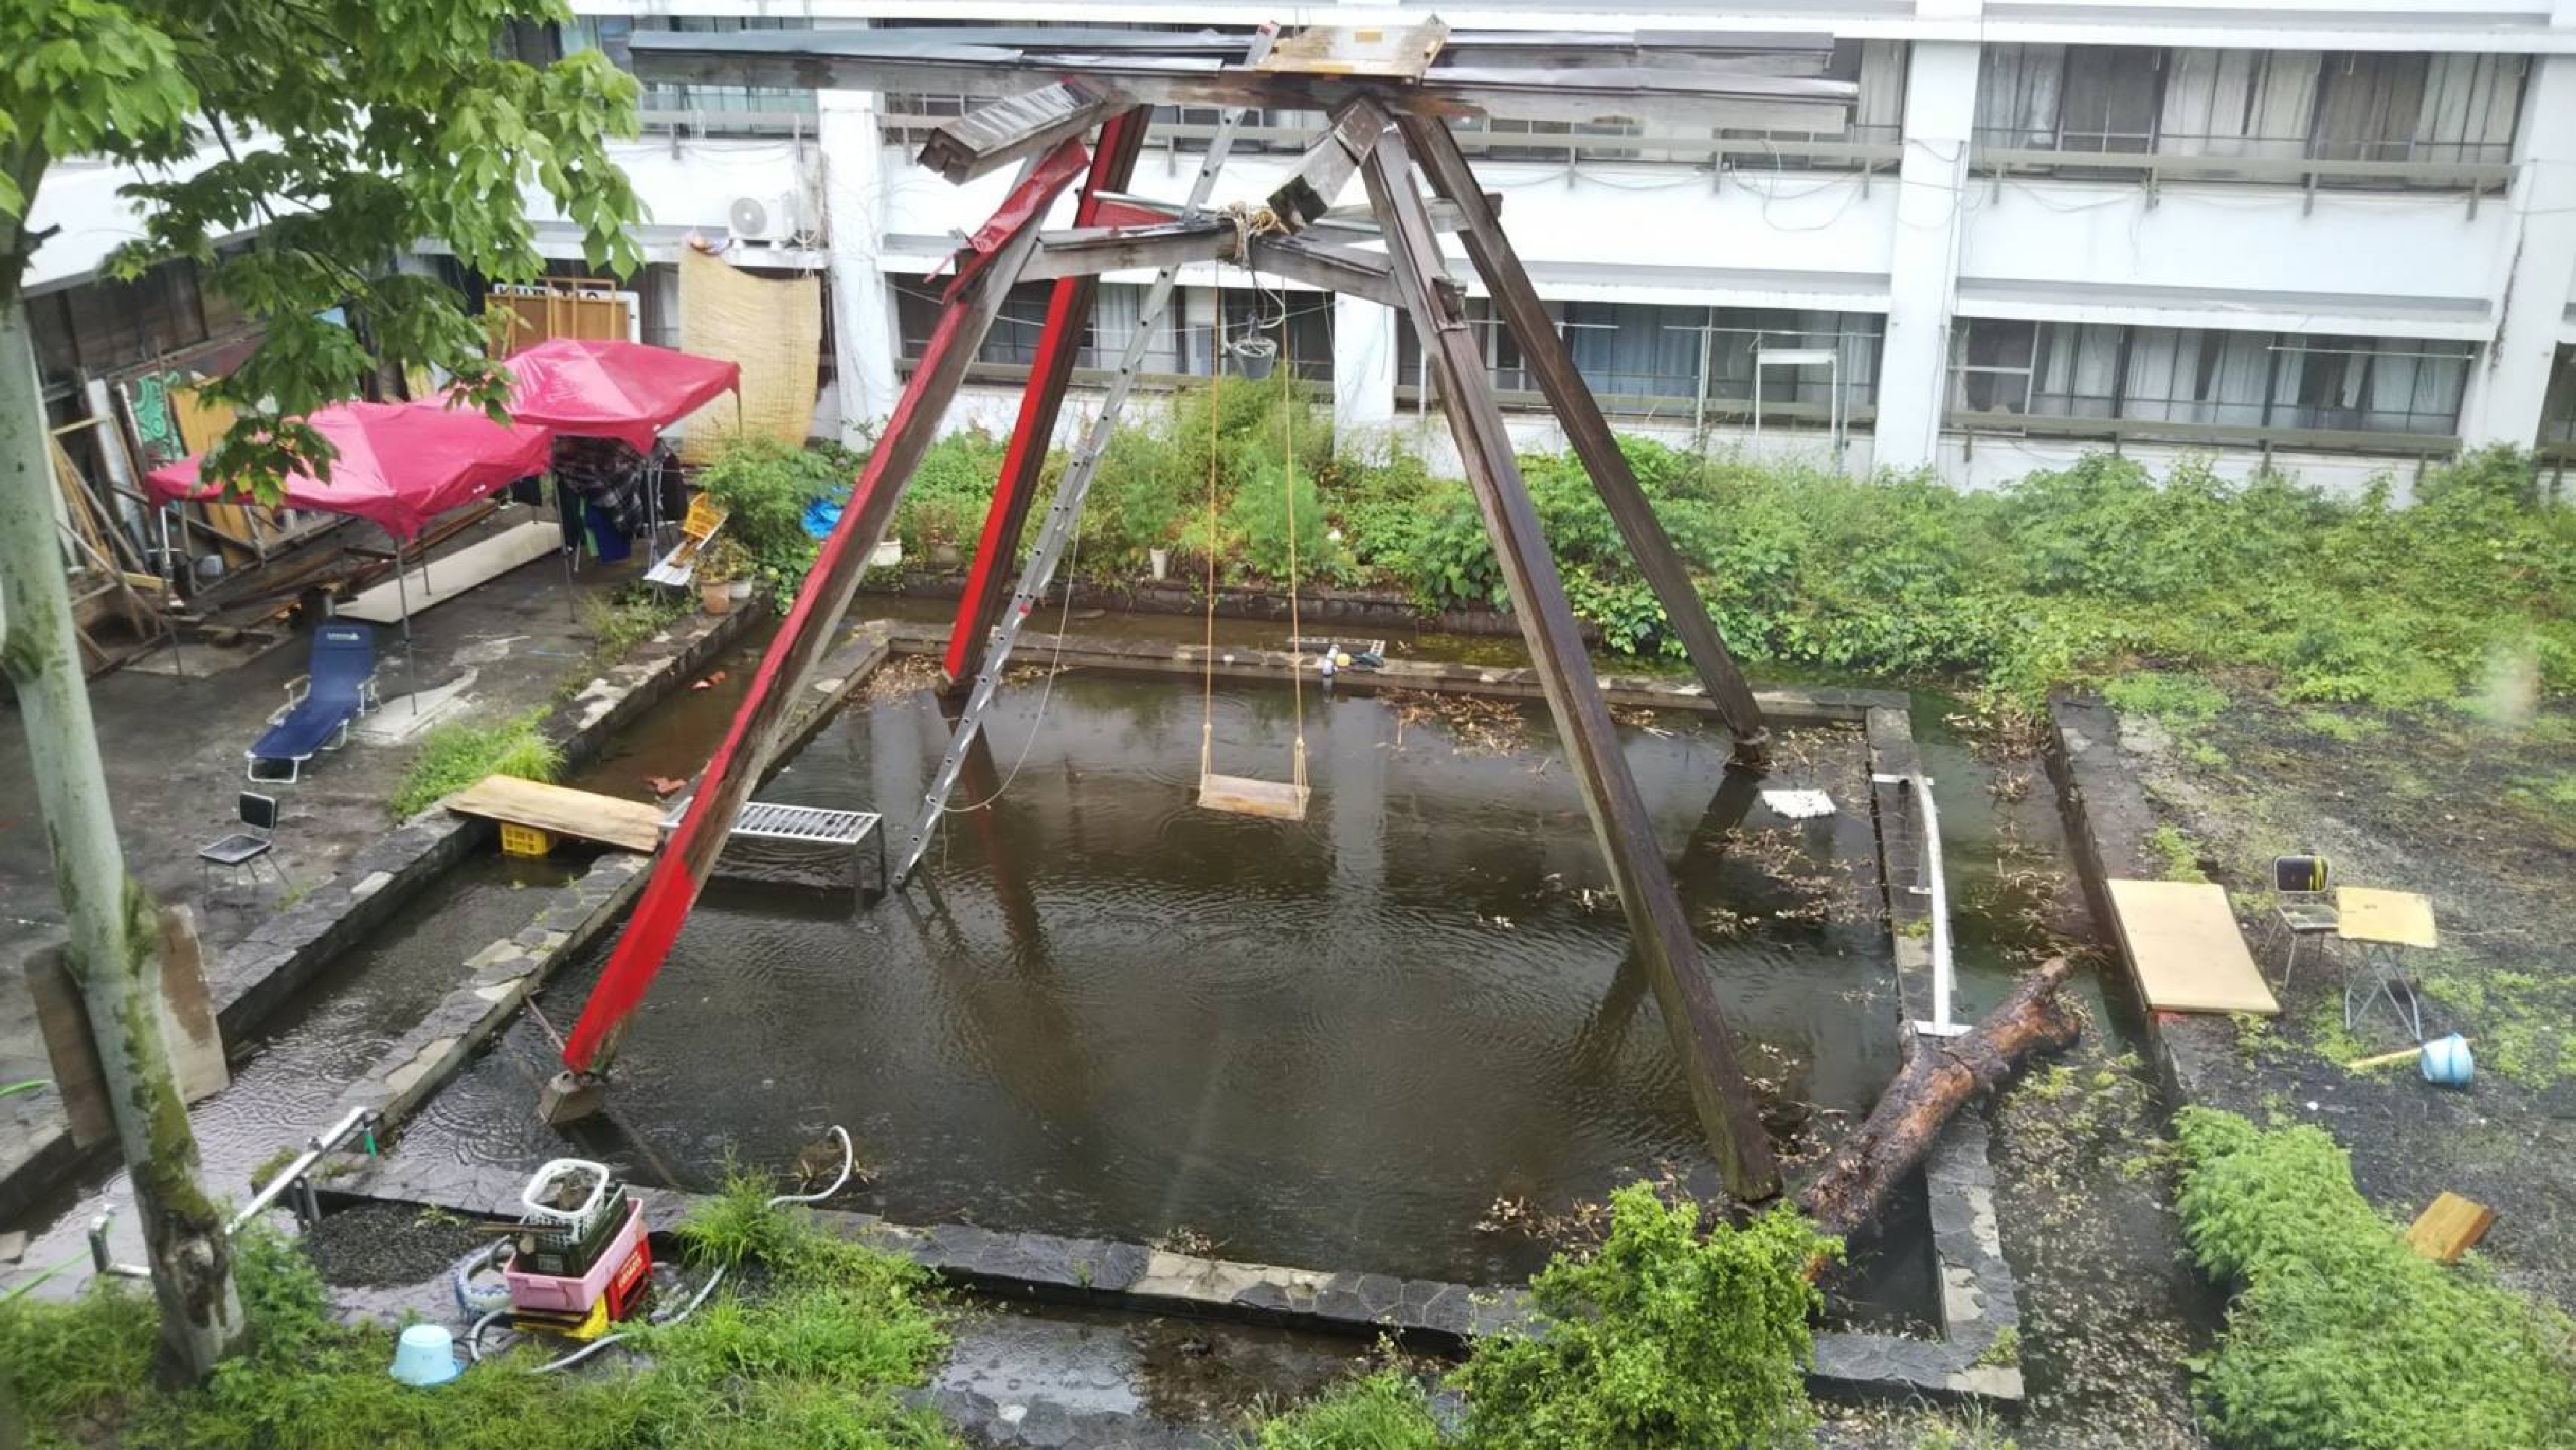
\includegraphics[width=6cm]{gazo/minseike.pdf}
    \caption*{{\small 民青池}}
  \end{figure}





%下は罫線があるバージョンの表
	% 	\begin{table}[htbp]
  %     \begin{tabular}{|lp{43zw}|}
  %       \hline
  %       \textbf{居室内}  & 冷蔵庫・テレビ・電気ケトル・炊飯器などは上回生が持っていたり、部屋で受け継がれていたりする場合がある。 防災上、石油ストーブは禁止。 寮内は屋上含め全面禁煙。 喫煙所が玄関脇にある。水道はない。 \\  \hline
  %       \textbf{談話室}  & おおむね各階に設けられた十数畳の部屋。 各階の集会場兼遊戯室となる。 使用状況は階によって様々だが、たいてい漫画・ゲームなどが置いてある。     \\ \hline
  %       \textbf{炊事場}  & 各階にある。 ガスコンロ・ガス湯沸かし器・流し・鏡などがある。                                                           \\ \hline
  %       \textbf{洗濯機}  & 各階にある。 各棟屋上には物干し場と乾燥機がある。                                                                   \\ \hline
  %       \textbf{トイレ}  & 各階にある。 水洗トイレ。 和・洋式どちらもある。 B棟一階には多目的トイレがある。C棟二階にはオールジェンダートイレがある。                             \\ \hline
  %       \textbf{食堂}   & 栄養士さんが考えたバランスのとれた食事を、日替わりで楽しめる。 食堂内には自動販売機、製氷機、電子レンジがある。 卓球台も置いてある。 食堂はコンパなど多くの催し物に使われる。    \\ \hline
  %       \textbf{事務室}  & 維持費の支払い、来客の対応などをする。 新聞各紙(京都・読売・朝日・毎日・日経) を閲覧できる。 ここでは常時寮生が事務室当番として電話の取次ぎや、郵便物の管理を行っている。     \\ \hline
  %       \textbf{シャワー} & A棟一階には男女別のシャワー個室があり、男子6基、女子2基ある。 料金は3分10円のプリペイドカード式。 ドライヤーもある。                              \\ \hline
  %       \textbf{ロビー}  & 食堂に準ずる交流の場。 コンパなどに利用される。                                                                    \\ \hline
  %       \textbf{音楽室}  & B棟地下にある、スタジオ兼ライブハウス。                                                                        \\ \hline
  %       \textbf{硬鉄庵}  & B棟地下にある、分厚い扉に守られた部屋。 警察権力からの防衛に特化している。                                                      \\ \hline
  %       \textbf{民青池}  & たまに飛び込む者がいる。 寮祭企画・みかん祭りの開催場所になったりもする。元々は防火用。   \\ \hline
  %       \textbf{娯楽}   & 食堂の卓球台、敷地内のバスケットゴール・フットサルコートなどに加え、部屋で受け継がれているものもある。        \\ \hline                                
  %   \end{tabular}
  % \end{table}

%     \begin{figure}[h]
%  	\begin{flushleft}
%	\includegraphics[scale=0.3]%{muc.pdf}
%	\end{flushleft}
%	\end{figure}

  \vspace{10mm}

  \section{募集要項} \label{sec:admission}

\index{にゅうりょう@入寮!ぼしゅう@---募集}
\komoku{募集対象}
京都大学の学生、大学院生\index{だいがくいんせい@大学院生}、研究生、その他本学に学籍のある者(科目等履修生、聴講生など)を対象とする。性別、国籍\index{こくせき@国籍|seealsopage{留学生}}は問わない。

\komoku{募集人数}
現在の空き人数(100名程度)を募集する。

\komoku{選考}
入寮希望者が募集人数を超えた場合には選考を行う。

\komoku{入寮基準}
寮自治活動を理解し、積極的に参加すること。

\komoku{選考方法}
部屋割りの都合上、選考は男女に分かれて行われる。また下記のように経済的に困窮している者および留学生には優先的に選考を行う。経済選考、留学生選考\index{りゅうがくせい@留学生}に応募した者は、経済選考・留学生選考に漏れた時点で自動的に一般選考にまわる。 


% Please add the following required packages to your document preamble:
% \usepackage{multirow}
\begin{table}[hbt]
  \begin{tabular}{|l|lp{40zw}|}
  \hline
  一般選考 & \multicolumn{2}{l|}{全員に対して抽選を行って選考する。} \\ \hline
  \multirow{3}{*}{特別選考} & \multicolumn{2}{l|}{一般選考に優先して行われる。} \\ \cline{2-3} 
   & 経済選考 & 経済的に困窮している者は、経済選考に出願できる。出願希望者は、出願参考書類の所定の欄に記入し、既定の書類(後述)を添えて提出すること。困窮状況が明らかな場合は優先的に入寮を認める。\index{けいざいてきこんきゅう@経済的困窮}\\ \cline{2-3} 
   & 留学生選考 & 留学生は経済選考で必要な証明書を提出するのが困難であること、また留学生が置かれている社会的状況を考慮し、留学生枠を設定する。経済的に困窮している留学生の入寮希望者は、留学生枠への応募が可能である。その際、留学生選考用書類も併せて提出する必要がある。応募者の総数が留学生枠を超えた場合は、留学生枠内で抽選を行う。\\ \hline
  \end{tabular}
  \end{table}

\komoku{出願書類}
\begin{table}[htb]
  \begin{tabular}{|l|p{43zw}|}
    \hline
    全員必要なもの & \vspace{-5mm}\begin{itemize}
        \item 学籍を確認できるもの(学生証・合格証明書)の写し。*受験生は面接時に受験票を持参し、入寮手続き時に合格証明書の写し等を提出して下さい。
        \item 入寮願(署名の上、顔写真を貼付)
        \item 同一世帯全員の住民票写し(発行から3ヶ月以内、マイナンバー記載の\textbf{ない}もの。役所窓口で「世帯全員分」と言えば貰えます。留学生は提出不要)
        \item 出願参考書類
    \end{itemize} \\ \hline
    経済選考 & 上記に加えて以下の書類を提出して下さい。
    \vspace{-3mm}
    \begin{itemize}
      \item 出願参考書類の所定の欄に経済状況(家族の人数、収入の有無、就学の状況など)についての説明をできるだけ詳細に記入すること。十分な情報が記されていない場合、経済選考に出願できない場合がある。
      \item 家族全員の所得(または家庭の経済状況)を示すことのできる公的機関の発行する証明書あるいはその写し (例:源泉徴収票、確定申告書、失業保険の給付証明書、住民税の免除証明書など。)
      \item 特別な事情がある場合には、そのことを詳しく書いた書類やそれを証明できる公的な書類
    \end{itemize}\vspace{-0.8cm} \\ \hline
    留学生選考 & 全員必要な書類(住民票を除く)に加えて留学生選考書類を提出
    \\ \hline
  \end{tabular}
\end{table}
\par 上記の書類を面接時に提出すること(原則面接日に提出すること。やむを得ず当日用意できない事情がある場合は、面接受付時にその旨を申し出たうえ、入寮手続きまでに必ず提出すること。)。なお、一度提出された書類はいかなる理由があろうと返却しない。
\par 入寮願、出願参考書類、留学生選考書類は熊野寮HPの「入寮希望者の方へ」ページ下部から入手するか、このパンフレットに挟み込まれているものを使用して下さい。

\vskip\baselineskip
\komoku{面接と見学}\index{にゅうりょう@入寮!めんせつ@---面接|textbf}
  \begin{itemize}
		\item 入寮を希望する者は、必ず入寮面接を受けなければならない。
    \item この面接は入寮希望者が予め寮自治について理解するために行われる。
    \item 面接の場に入寮希望者本人以外は同席できない(付添人には面接中の待合スペースを用意している)。
    \item 面接による選考は、あまりに寮自治への理解がないと判断される場合を除いて行わない。
    \item 面接は\emphbf{熊野寮食堂にて}以下の日程で行われる。\emphbf{予約等は必要ない}ので都合の良い時間に来ること。\\
    (2月の日程と3月の日程で受付終了時間が異なるので注意)
      \begin{itemize}
      % TODO 日付曜日を変える
        \item 2月25日(火)、26日(水):午前10時から正午、および午後1時から午後7時
        \item 3月10日(月):午前10時から正午、および午後1時から午後7時
        \item 3月11日(火)、12日(水):午前10時から正午、および午後1時から午後5時
      \end{itemize}
    \item 面接の所要時間は1〜2時間程度。また面接後に寮内の見学をすることができる(付添人の同伴可能)。
	  \item \emphbf{京都大学を受験しているものは合否が判明してなくとも面接を受けることができる}。ただし不合格であった者の入寮は認められない。
    \end{itemize}
	
%\newpage % これはレイアウトの都合なのでいらなさそうなら消す
		
\komoku{選考後の流れ}
	\begin{enumerate}
		\item 当落発表
      % TODO 日付曜日を変える
		3月14日(金)夜に選考を行い、翌15日(土)に全ての出願者に選考結果を電話で通知する。
		\item 繰り上げ当選

 		落選者は、キャンセル待ちに登録することができる。選考結果の連絡を受けた際に申し込むこと。

 		選考当選者のキャンセルが発生するたびに、キャンセル待ちに登録した者の中から、繰り上げで追加の当選者が確定していく。追加で当選した者には、当選した時点で電話で連絡する。
	\end{enumerate}

\newpage 
\komoku{入寮手続き}
		期日までに行われなければ入寮資格を失う。やむを得ず面接日に不足書類があった者は手続きまでに必ず書類を持参すること。
		
		例年、入寮手続き最終日を中心に手続き希望者が殺到して長蛇の列ができ、事務員さんにも負担がかかっています。新入寮生の皆さんには、以下の3点を注意していただくようお願いしたいです。
		\begin{itemize}
		    \item \emphbf{必ずしも居住開始日に手続きする必要はありません}。入居日から手続き締め切り日までのうちで出来るだけ窓口が空いている時間帯を選んで手続きに来てください。また、とくに最終日は混むので出来るだけその前までに済ませてください。
		    \item 入寮手続きの際に保護者が同伴するのは、出来るだけ遠慮していただくようお願いします。
		\end{itemize}
        
\komoku{受付日}  以下の日程で受け付けている。
      % TODO 日付曜日を変える
\begin{table}[h]
  \begin{tabular}{|l|c|c|c|}
    \hline
    受付日 & 曜日  & \multicolumn{2}{|c|}{受付時間}                  \\ \hline \hline
    
    3月24日 & 月 & 9:45〜12:45 & $ \times $   \\ \hline
    3月25日 & 火 & 9:45〜12:45 & 14:00〜15:30\\ \hline
    3月26日 & 水 & 9:45〜12:45 & $ \times $\\ \hline
    3月27日 & 木 & 9:45〜12:45 & 14:00〜15:30  \\ \hline
    3月28日 & 金 & 9:45〜12:45 & 14:00〜15:30  \\ \hline
     \hline
  \end{tabular}
\end{table}

\komoku{入寮オリエンテーション}
	3月30日(土)13時からの入寮オリエンテーション\index{にゅうりょう@入寮!おりえんてーしょん@---オリエンテーション}に参加すること。また、これに不参加の者は強制退寮となる場合があるので、必ず参加のこと。(所要時間:4〜5時間程度)

\index{にゅうりょう@入寮!ぼしゅう@---募集}

  \newpage
  \section{お問い合わせ・ご相談}\label{sec:otoiawase}
熊野寮では、寮内外からの問い合わせ・相談に対して複数の窓口を設けています。ここでは、入寮を希望するみなさんに向けて、熊野寮の問い合わせ先・相談体制についてご紹介します。\index{くまのりょう@熊野寮!のれんらくさき@---の連絡先}

\subsection{熊野寮自治会}
\begin{itemize}
\item メールアドレス:\url{info@kumano-ryo.com}
\item 電話番号:075--751--4050、075--751--4051
\item 受付時間:8:00~23:00
\end{itemize}
\noindent ※熊野寮は、業務が苦手であったり時間がかかったりする寮生含め、皆が当番\index{じむしつ@事務室!とうばん@---当番}に入り運営される自治寮です。そのため、電話の応対に際しご不便をおかけすることがあります。ご理解のほど宜しくお願い致します。

\subsection{入寮に関するお問い合わせ}
\noindent 入寮選考担当のメールアドレス:\url{interview@kumano-ryo.com}

返信まで3日から4日程度のお時間を頂いております。お急ぎの用件に関しましては、熊野寮自治会の項目に記載の番号まで、お電話にてお問い合わせください。直接来ていただいて、寮内を見学することもできます。寮生が案内しますので、入り口右側の事務室にお声かけください。\index{にゅうりょう@入寮!にかんするといあわせ@---に関する問い合わせ} 

\subsection{人権擁護部相談メール}
\noindent 人権擁護部のメールアドレス:\url{kumano.jinken@gmail.com}

人権擁護部では、すべての寮生が不快な思いをせず生活できるよう、様々な取り組みを行っています。入寮後、寮内で生じたトラブル\index{とらぶる@トラブル}や生活上の悩みなどがあれば上記のメールアドレスへお気軽にご相談ください。

また、見学・入寮選考などで来寮の際にハラスメント被害を受けた/見聞きした場合や、入寮にあたってプライバシー\index{ぷらいばしー@プライバシー}に関わるご相談がある場合などには、相談メールまでご連絡ください。

\subsection{女子寮生向けハラスメント相談窓口}\index{じょしりょうせい@女子寮生!むけはらすめんとそうだんまどぐち@---向けハラスメント相談窓口}
\kkomoku{当相談窓口について}

「この人には絶対に相談したことを知られたくない!」「異性相手に絶対に知られたくない悩みがある」「そもそも相談してもいいのかわからない」\index{はらすめんと@ハラスメント|seealsopage{セクハラ, アルハラ, アカハラ}}

寮では(大変残念なことではありますが)このような気持ちを抱える事態が発生することがあります。この相談窓口は、“女子寮生向け“と銘打ってありますが、女子トイレと女子シャワー室を使う寮生に向けて作られたものです\index{じょしりょうせい@女子寮生}。相談員は全員が女子寮生です。セクハラ\index{せくはら@セクハラ}、アルハラ\index{あるはら@アルハラ}、その他トラブルなど、もし将来熊野寮に住んでいて困ったことがあったら、この相談窓口があることを思い出してください。

\kkomoku{相談窓口の使い方}

熊野寮の女子トイレ\index{といれ@トイレ}、女子シャワー室\index{しゃわー@シャワー}、そしてC棟のオールジェンダートイレには、この相談窓口の相談員のLINEのQRコードが貼りだしてあります。自分が相談しやすいと感じる人を選んで、相談のLINEを送ってください。明確に「ハラスメントだ!」と思うようなことでなくても大丈夫です。まずは相談してみてください。また、「この人に知られたらどうしよう」という心配も無用です。相談した内容を誰に共有するか、誰に対応してもらうかは、事態が解決するまで相談した人に決定権があります。




\chapter{寮での生活}

  \section{寮食堂と寮生}	\label{sec:cafeteria}\index{りょうしょく@寮食|textbf}
 	熊野寮には、全国の学生寮でも数少ない寮食堂があります。基本的に大学の授業がある平日、朝昼夜の三食が用意され、朝は7時半〜10時、昼は12時〜13時、夜は17時〜17時45分が喫食時間としています。これを見て、「え、そんなに食べる時間短いの? 」と思った方もいるでしょう。ご安心を、そういったご飯の時間内には食べに来られない人のために昼と夜は「残置」\index{りょうしょく@寮食!のざんち@---の残置}というシステムを作ってあり、昼は15時まで、夜は22時までに食べにくるという条件の下で寮食を取り置くことができます! さらに、寮食には利点がいっぱいあります!

  \subsection{寮食は栄養満点! }\index{りょうしょく@寮食!のえいよう@---の栄養}
 	  まず、寮食堂には栄養士の方がいらっしゃり、毎日の栄養計算から献立を作って下さっています。しかもボリュームも満点! しっかり三食食べれば二十歳の成人男性が一日に必要な栄養素を摂取できるのです。朝はパンと乳製品、昼は野菜たっぷりのご飯、夜は主菜を中心とした汁物、副菜二品セット。寮食三食で一日分のビタミン、ミネラルも摂取できるのです。今の若い時分にしっかり栄養を摂っておかないと将来生活習慣病の予備軍になってしまいますが、寮食なら安心ですね。

	\subsection{寮食は安全安心! }
    寮食は安全面にも気を配っています。衛生面はもちろんのこと、使う材料にも気を付けており、肉はほとんど国産、野菜は京野菜をふんだんに使用し、卵は餌から管理されているものを使い、添加物も極力省いています。栄養面でも安全性の面でも身体に良い寮食、これは食べるしかありませんね!

	\subsection{寮食は安い!}\index{りょうしょく@寮食!のねだん@---の値段}
		栄養満点ボリューム満点、おまけに安全安心そんな寮食。でもお高いんでしょう? いえいえ、そんなことはありません! \emphbf{朝は170円、昼は260円、夜は390円と破格! }しかしながらその裏には厨房の栄養士さんや調理員さんの多大なる努力があります。食材を大量購入し、その材料が無駄にならないような調理法、献立を考えた上で栄養も毎日しっかり保つ。さらには夏の冷麺や素麺、冬の鍋物やシチュー、おまけに節分(2月3日)などの季節を感じさせるメニューも登場します。


		\subsection{寮食堂は交流の場}
		食堂と言えばご飯を食べるところ。もちろんそれが食堂の一番の意味ですが、熊野寮食堂は様々な寮生と知り合い交流する場でもあります。熊野寮の食堂は24時間365日開放されています。その管理・運営は寮生と厨房員さんの二人三脚で行われます。なので自分たちの好きな時に自分たちの好きなことができる。これこそまさに自治であり、寮食堂とは自治を象徴する場所なのです! 他愛もない話から昨今の政治の動きなどの難しい話まで、色んな話をしながら寮食を食べるのもあり。時々企画されるコンパやイベント事で朝まで交流するのもあり。炊事当番(食器洗い当番とも言う) では寮生や厨房の方と一緒に働く。自分たちの意志で自由にできる場所です。そしてその意思決定には外部からの干渉は受けません! 友達ができそうになくボッチになりがちな人でも、寮食を食べたりコンパ\index{こんぱ@コンパ}やイベントに参加したりすれば、楽しい出会いが待っていることでしょう。

		ここだけでは熊野寮食堂の素晴らしさは語りつくせません。入寮した暁には、寮食共々是非食堂を利用して有意義な大学生活を送って下さい。



% Please add the following required packages to your document preamble:
% \usepackage{multirow}

\begin{table}[ht]
  {\small
  \caption*{一週間の寮食メニュー(一例)}
  \begin{tabular}{|l|p{9zw}p{9zw}p{9zw}p{9zw}p{9zw}|}
  \hline
   & \multicolumn{1}{l|}{月曜日} & \multicolumn{1}{l|}{火曜日} & \multicolumn{1}{l|}{水曜日} & \multicolumn{1}{l|}{木曜日} & 金曜日 \\ \hline
  \multirow{2}{*}{朝食} & \multicolumn{5}{c|}{パン、牛乳・乳酸飲料・野菜ジュースから一つ選択、チーズ・卵から一つ選択} \\
   & \multicolumn{5}{c|}{*数量限定でカット野菜が用意されており、食パンとチーズと組み合わせピザトーストが作れる} \\ \hline
  \multirow{7}{*}{昼食} & \multicolumn{1}{l|}{そぼろ丼} & \multicolumn{1}{l|}{高菜炒飯} & \multicolumn{1}{l|}{他人丼} & \multicolumn{1}{l|}{オムライス} & 根菜コロッケカレー \\
   & \multicolumn{1}{l|}{味噌汁} & \multicolumn{1}{l|}{サラダ} & \multicolumn{1}{l|}{胡麻和え} & \multicolumn{1}{l|}{サラダ} & ヨーグルトサラダ \\
   & \multicolumn{1}{l|}{} & \multicolumn{1}{l|}{スープ} & \multicolumn{1}{l|}{} & \multicolumn{1}{l|}{スープ} &  \\ \cline{2-6} 
   & \multicolumn{1}{l|}{} & \multicolumn{1}{l|}{スパゲッティ・ミートソース} & \multicolumn{1}{l|}{} & \multicolumn{1}{l|}{豚骨ラーメン} &  \\
   & \multicolumn{1}{l|}{} & \multicolumn{1}{l|}{} & \multicolumn{1}{l|}{} & \multicolumn{1}{l|}{} &  \\
   & \multicolumn{1}{l|}{} & \multicolumn{1}{l|}{} & \multicolumn{1}{l|}{} & \multicolumn{1}{l|}{} &  \\ \cline{2-6} 
   & \multicolumn{5}{c|}{*火曜日と木曜日の昼食は、ご飯と麺の2種類のメニューから選択} \\ \hline
  \multirow{6}{*}{夕食} & \multicolumn{1}{l|}{鰆の柚子かぶら餡かけ} & \multicolumn{1}{l|}{豚肉の照り焼き} & \multicolumn{1}{l|}{赤魚のきのこ餡かけ} & \multicolumn{1}{l|}{プルコギ} & 煮込みハンバーグ \\
   & \multicolumn{1}{l|}{ボイルキャベツ} & \multicolumn{1}{l|}{ボイルキャベツ} & \multicolumn{1}{l|}{ボイルキャベツ} & \multicolumn{1}{l|}{ボイルキャベツ} & ボイルキャベツ \\
   & \multicolumn{1}{l|}{かぼちゃの煮物} & \multicolumn{1}{l|}{ソテー} & \multicolumn{1}{l|}{鶏じゃが} & \multicolumn{1}{l|}{五目煮豆} & オイスター炒め \\
   & \multicolumn{1}{l|}{お浸し} & \multicolumn{1}{l|}{酢の物} & \multicolumn{1}{l|}{お浸し} & \multicolumn{1}{l|}{ゆかり和え} & ピーナツ和え \\
   & \multicolumn{1}{l|}{すまし汁} & \multicolumn{1}{l|}{味噌汁} & \multicolumn{1}{l|}{味噌汁} & \multicolumn{1}{l|}{すまし汁} & 味噌汁 \\ \cline{2-6} 
   & \multicolumn{5}{c|}{*夕食にはご飯がつきます。} \\ \hline
  \end{tabular}
  }
\end{table}
\index{りょうしょく@寮食!めにゅー@---メニュー}


  


寮生が有志でほぼ毎日、寮食のメニューや写真をあげているX(旧twitter)アカウント\index{ついったー@ツイッター!のりょうかんけいあかうんと@---の寮関係アカウント}もあります。興味があればごらんください!

\begin{figure}[h]
  \begin{minipage}[b]{0.5\textwidth}
    \centering
    
\includegraphics[width=3cm]{gazo/QR_ryoshoku_bot.png}
    \subcaption{\url{https://twitter.com/ryosyoku_buono}
    \\熊野寮寮食bot Twitter(\url{@ryosyoku_buono})}
  \end{minipage}
  \begin{minipage}[b]{0.5\textwidth}
    \centering
    
\includegraphics[width=3cm]{gazo/QR_ajiri.png}
    \subcaption{\url{https://bit.ly/3rL87Vk}\\ 熊野あじり Twitter\url{@kumano_ajiri}}
  \end{minipage}
\end{figure}


\begin{figure}[H]
  \centering
  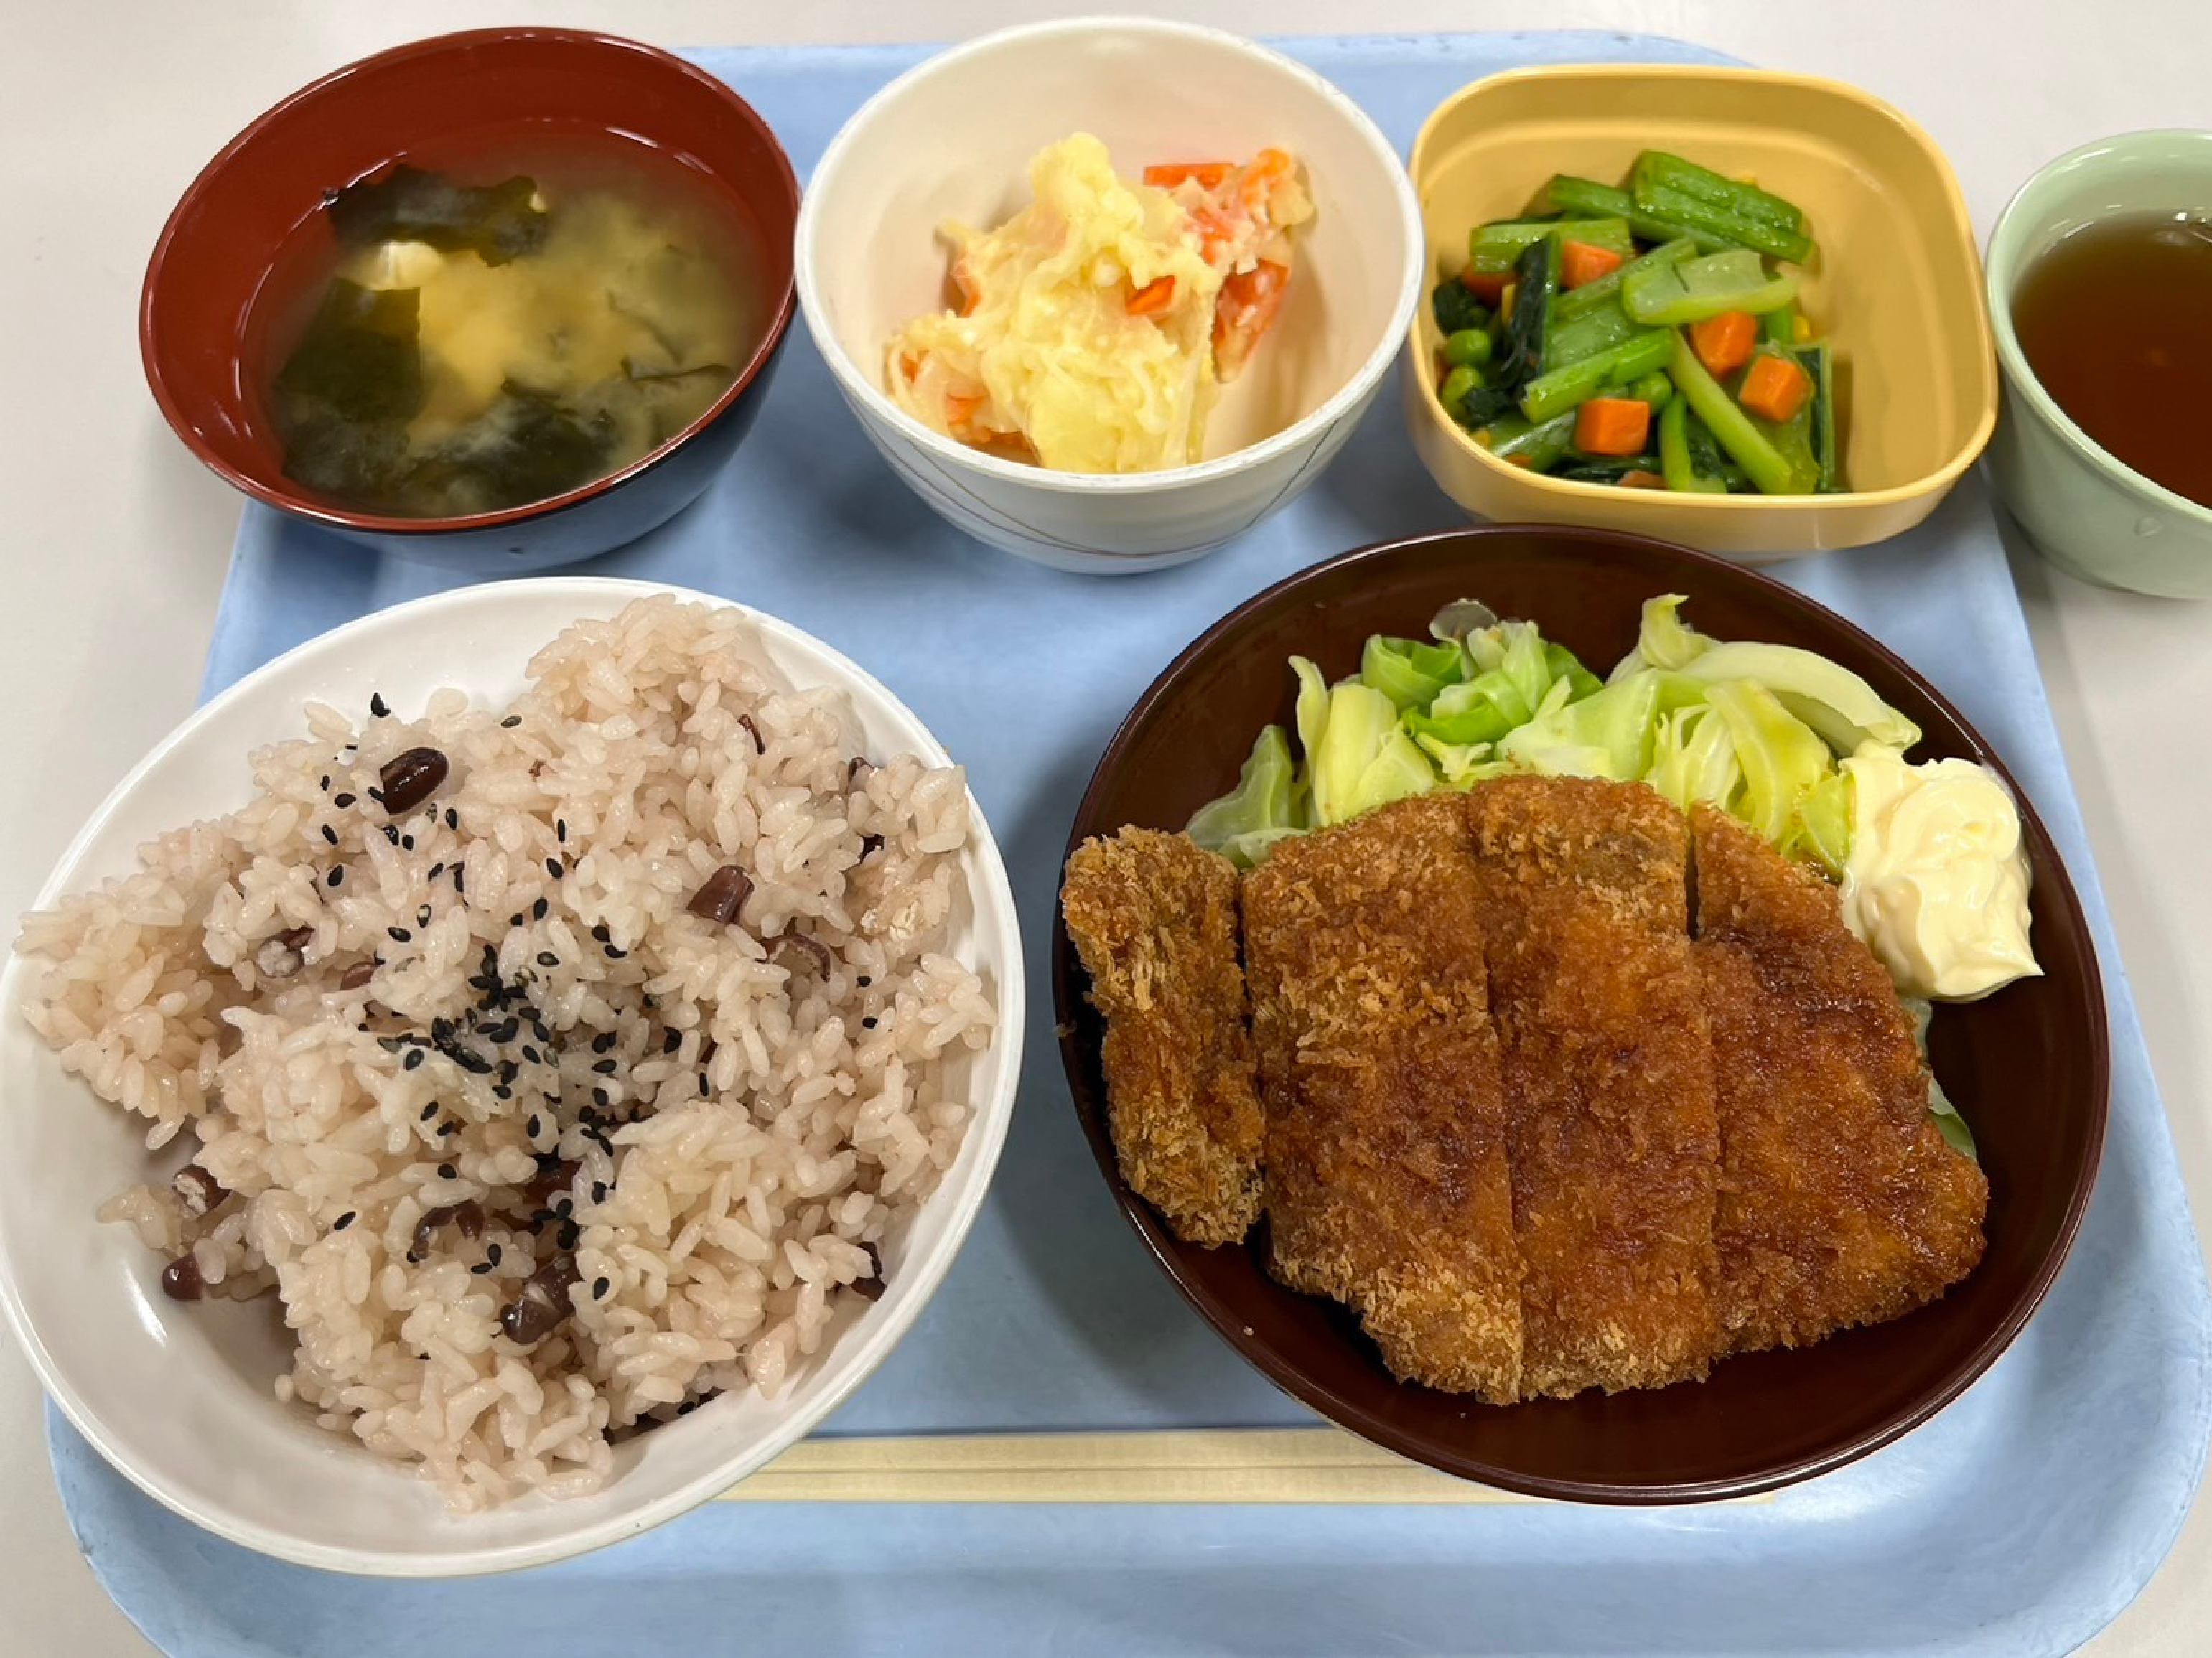
\includegraphics[width=5cm]{gazo/sekihan.pdf}
  \subcaption{{\small この日の夕食は赤飯に豚カツの豪華メニュー}}
\end{figure}

  \newpage

  \section{音楽室}\label{sec:MUC}\index{おんがくしつ@音楽室|textbf}


ハローこんにちは!熊野寮に並みいるヘンテコスペースの中でも特にブッ飛んだ、音楽室の紹介をするぜ!

既にご存知かもしれないが、熊野寮は世にも珍しい、音楽室があるブッ飛んだ寮なのだ!!そして音楽室ユーザー全体から成る、音楽室を自分たちの手で管理、運営するブッ飛んだ団体が我々
\vskip\baselineskip

{\huge MUC : \textit{Music room Users' Conference}}\\
なのである!\index{MUC@MUC(音楽室利用者会議)}\index{おんがくしつりようしゃかいぎ@音楽室利用者会議|see{MUC}}

音楽室といっても学校の音楽室のようなものでなく、アンプやキーボード、ドラムなどのバンド用の機材がそろったブッ飛んだ空間だ。バンド演奏を中心に使われているが、歌の練習、ダンスの練習にも使われている。つまりは実質フリースペース!ついでに利用料もフリー!

また、その発表の場として寮内で開かれるブッ飛んだライブに出ることもできるぞ!ライブはほぼ月1でやってるから最早やりすぎって感じだ!毎回ライブでは寮内の音楽好きが集まってめちゃめちゃ盛り上がるぜ!出演バンドは例えばアジカンやKing Gnuなどロックのコピバンが多いな!たくさんライブに出てブッ飛んだ時間を作ろう!

じゃあMUCって具体的に何すんのかな?それは大きく分けて3つある。一つは音楽室機材のブッ飛んだメンテ、管理。一つはライブの準備。そして毎週月曜のブッ飛んだミーティングだ。いずれも詳しく書くことは控えておくが、たくさんの人と交流できるブッ飛んだ仕事だ!音楽機材に強くなれたりもするぜ!

音楽室はどうやったら使えるようになるのかって?それは毎週月曜日の21:30からやってるMUC会議に出ればOKだ!ちなみに音楽室は寮生じゃなくても会議に来るだけで使えるぜ!音楽好きな奴はMUC会議に来てくれよな!

バンドでライブ\index{らいぶ@ライブ|textbf}がしたい?ダンスでクールに決めたい?うんうん!大いに歓迎しよう。ちょっとだけ興味あるけど… うんうん!君も大歓迎だ!ブッ飛んだ紹介は以上だ!諸君!MUCで会おうぜ!





\begin{figure}[bh]
	\centering
	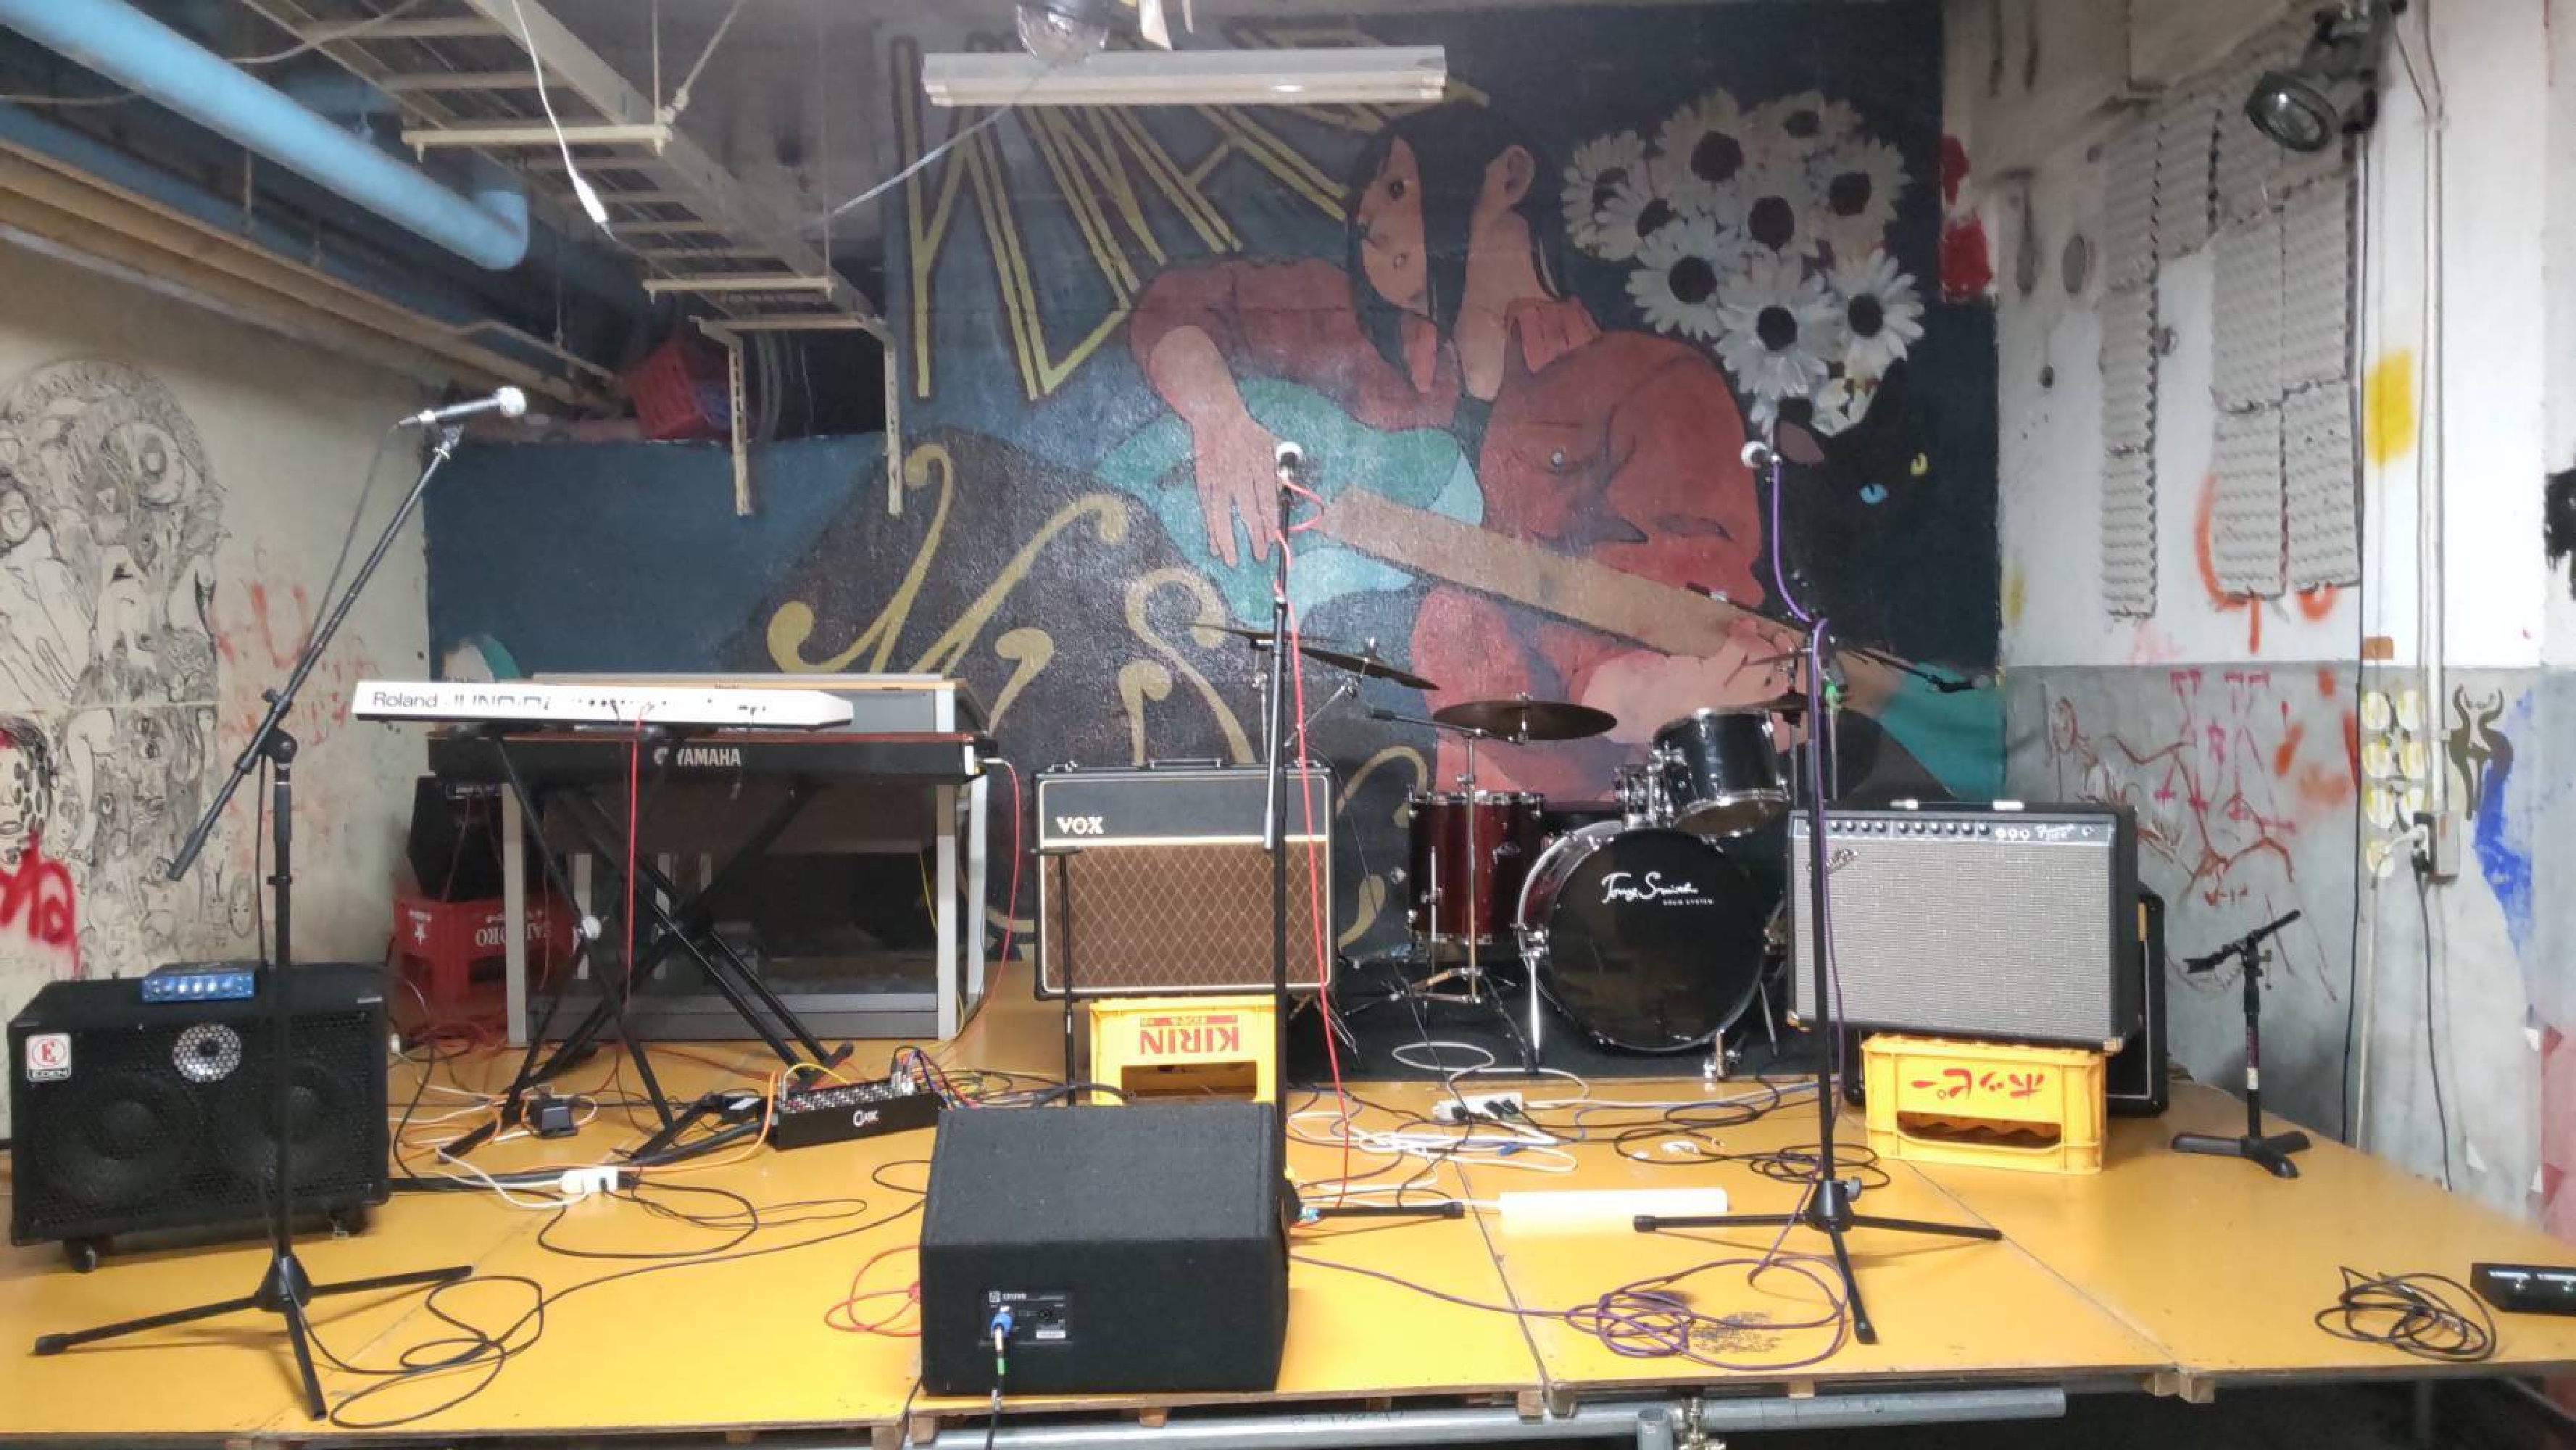
\includegraphics[width=16cm]{gazo/music_room.pdf}
\end{figure}

  \newpage

  \section{ハラスメント加害者にならないために}\index{はらすめんと@ハラスメント|textbf}
\label{sec:harassment}
  \bunsekisha{文責}{人権擁護部\footnote{人権擁護部では, すべての寮生が不快な思いをせず生活できるよう, 様々な取り組みを行っています.}}

  \subsection{人の体にさわらない. }
  「同性同士のボディタッチは友情の証」, 「異性へのさりげないボディタッチはモテるコツ」などと思っていませんか?その行為は人を不快にさせるには十分です. やめましょう.
  
  \subsection{公共スペースでは下ネタ・猥談はしない. }
  下ネタ・猥談は不快になる人がいます. 過度のいじりや不謹慎ネタなども同様です. その場のノリや勢いだけで発言しないように気を付けましょう. \index{しもねたをしない@下ネタ(をしない)}
  
  \subsection{人の容姿, 私生活を評価することを言わない. }
  人の容姿や私生活はその人のもの, 他の人がとやかく言ったり評価したりすることではありません. 
  
  \subsection{「女性/男性はこうである」など性別によって人のあり方を決めつけない.}
  「女の子なのに化粧しないの? 」とか「男性が奢らなきゃ」とか思ったことありませんか? 性別による一方的な決めつけに苦しめられている人がいます. 性別にかかわらず自分の生き方は自分で決めるものであって, 他の人が押し付けるものではありません. 
  
  \subsection{怒られない雰囲気に甘えない. }
  相手や周囲がはっきりとNGサインを出さなければOKではありません. 嫌な思いをしていても, その場の雰囲気に合わせてニコニコしているだけかもしれません. 
  
  \subsection{大学生には彼氏/彼女がいて当たり前と思わない. }\index{かれし@彼氏}\index{かのじょ@彼女}\index{せくはら@セクハラ}
  「恋人欲しい!」と思って気になる人にグイグイいくと, 相手はけっこう怖い思いをしているかも. 寮は生活の場であって出会いの場ではありません.
  
  \subsection{もし「それ問題だよ」と指摘されたら}
  「意図」で反論しないようにしましょう. 相手を傷つけてしまったり不快にさせてしまったりした場合, あなたがどのような意図でそれを行ったかは全く関係ありません. 自分の行動の何を問題だと指摘されているのか, まずは丁寧に聞きましょう. またそれと同時に, 周囲の人が加害者の意図を取沙汰して責めないようにすることも忘れてはならないことです. 

  

  \newpage
  
  
%\subsectionのタイトルを◯なしに

\section{熊野寮祭 ―これが私たちのやり方だ―}\label{sec:ryosai}\index{くまのりょうさい@熊野寮祭|textbf}
\bunsekisha{文責}{熊野寮祭実行委員会}

\subsecnomaru

 はじめに、皆さんが寮に入る理由には様々なものがあると思います。安いから、コンパとか楽しそうだから、友達がたくさん欲しいから、自治活動をしたいから、、。どれもこれもこの寮の魅力であります。そんな皆さん全員にぜひとも紹介したいのが、年に一度、11月末から12月初めにかけて行われる全寮を挙げたビッグイベント、「熊野寮祭」です。

 補足として、入寮したばかりの新入寮生は、前述の「くまのまつり」と今から述べる「熊野寮祭」をよく混同させてしまうのですが、それぞれ違うお祭りです。「くまのまつり」\index{くまのまつり}は、一年のうちで春夏秋の3度行われ、地域の方々に出店していただいたり、ステージに出演していただいたり、一緒に盆踊りを踊ったりと、寮生と地域の方々が織り成すという点で、地域色の濃いお祭りになっています\index{ちいきとのれんたい@地域との連帯}。執筆者自身、「くまのまつり」も大好きなのですが、「熊野寮祭」はそれとはちょっと違うお祭りになります。

 先ほど述べた通り、「熊野寮祭」(以下、寮祭と記す)は、年に一度、11月末から12月初めにかけての10日間で行われます。その規模は、寮内だけに留まらず、京都市、京都府、さらには全国にかけて広がり、「カオスの祭典」とも形容される通り、寮生の考案した企画が各所で乱立するお祭りとなります。2024年度の寮祭では、なんと500もの企画が集まりました。\par ここではいくつかの目玉企画をご紹介したいと思います。\index{くまのりょうさい@熊野寮祭!きかく@---企画|(}



\subsection{時計台コンパ}
\index{とけいだいこんぱ@---時計台コンパ}
寮祭初日の昼休みにクスノキ前で行われるコンパです。2024年度では、クスノキ前にでっかいタテカンを建て、鏡開きとともに寮祭の開幕を高らかに宣言し、ライブをしたり、お菓子を投げたり、風船を飛ばしたり、鍋料理を出したり、さらにはお酒を配ったりしました。このコンパにはキャンパスの学生だけでなく、職員の皆さんも多く詰めかけ、大いに盛り上げてくれます()。


\subsection{エクストリーム帰寮}
\index{えくすとりーむきりょう@エクストリーム帰寮}
参加者は夜中に全国の各所へと飛ばされ、無一文で寮に帰ってくるように命じられます。寮祭が全国規模で行われるとはこういうことです。2023年度ではなんと200 km離れた場所から帰寮した猛者もいました。



\subsection{四条大運動会}

三条河原でのラジオ体操に始まり、三条ジャンカラ前の広場での騎馬戦、新京極通500mあまりを疾風のごとく南下する二人三脚、借り物競争、四条河原町交差点を舞台とするパン喰い競争、そして四条大橋での大綱引きでフィナーレとなります。ここでは多くの警察が詰めかけ、大いに盛り上げてくれます()。



\subsection{大階段グリコ}

舞台はイルミネーションの輝く京都駅の大階段。そこらへんを歩いている通行人、観光客にじゃんけんを仕掛け、誰よりも速く頂点に登ることを目指します。コミュ力と少しの強運が勝負を左右します。

\subsection{AB棟間綱引き}

寮のA棟とB棟に綱をかけて引き合います。C棟民をいかに仲間にできるかが勝敗を左右します。あおり合戦と稀に起こる裏切りが見所です。

\subsection{鴨川イカダレース}

鴨川を自前のイカダで三条から四条まで南下します。壊れてしまうと極寒の川を泳ぐ羽目になります。


\subsection{}

他にも、演劇\index{えんげき@演劇}、アニメや映画の上映会\index{えいが@映画}、種々のコンパ、、。様々な企画が思いつくままに開かれています。個人の単なる思い付きがこの祭では様々な形に変貌します。皆さんの日々の「やってみたい」がこの祭にて実現されます。あなたの企画を寮生は支え、最高に盛り上げ、最高に楽しんでくれます。ここに人の温かみや寮の面白さを再認識し、もっとこの寮のことが好きになるに違いありません。

普段、自分たちの日常が広がる熊野寮が、この期間だけは非日常的な空間へと変貌します。京都大学の学祭、NF\index{NF@NF(11月祭)}が「熊野寮祭の前夜祭」だと称されてしまうほどに、2024年度の寮祭も多くの寮外生を動員し、大変盛り上がりました。また、前述の「くまのまつり」と同様、寮祭パンフに広告を載せるスポンサーになってもらったり、実際に寮祭に遊びに来てもらったりする形で、地域の方々や様々なサークルからのご協力も頂いて、このように毎年大規模に開催することができています。

現在、京都大学は学生の活動に様々な規制をかけています。いわゆる弾圧です\index{だいがくとうきょく@大学当局!によるだんあつ@---による弾圧}。サークルは自由に活動させてもらえず、京大構内や百万遍交差点\index{ひゃくまんべん@百万遍}に設置したタテカン\index{たてかん@タテカン}は即撤去され、、。昔できていたことが自由にできなくなってしまったのです。実際、寮祭にも、特に時計台コンパや総長室突入など京大構内で実施する企画や、四条大運動会など地域を舞台とする企画には弾圧がかかります。かつては自由に行われていた時計台占拠にも現在では激しい弾圧がかかります。京大が謳っている「自由な学風」\index{じゆうのがくふう@自由の学風}は失われつつあるといえます。しかし、そんな中でも熊野寮は長い年月をかけて培ってきた自治のもとに、弾圧に負けることなく企画を貫徹します。京大の、さらには全人類の自由やカオスとを取り戻すために、私たちはこの祭を全力で盛り上げ、全力で楽しみます。これが私たち熊野寮のやり方です。これが私たち熊野寮の大いなる魅力です。皆さんが京大に求める自由やカオスはここにあります。皆さんも私たちと一緒にそれを体現しましょう!次なる主役は君たちだ!
\index{くまのりょうさい@熊野寮祭!きかく@---企画|)}


\begin{figure}[H]
  \centering
  \includegraphics[height=5cm, angle=-90]{gazo/guriko.pdf}%何故か横倒しになるので、angleオプションを付けている。
  \subcaption{{\small 京都駅大階段グリコ}}
  
\end{figure}

\subsecdefault
%\subsectionのデザインを元に戻す




  
  \newpage
  
  
\section{くまのまつり ― 地域と共に創るお祭り}
\label{sec:kumanomaturi}\index{くまのまつり|textbf}

\subsection{くまのまつりとは}

熊野寮では, 5月, 8月, 11月に「くまのまつり」というお祭を開催しています. このお祭は, もともとは地域の商店の方々が2010年に立ち上げ, 翌年から寮自治会との共催で開いているものです. これは地域と一緒につくるお祭りであり, 寮自治会としては寮外との連帯を目指すためのお祭です.\index{ちいきとのれんたい@地域との連帯|textbf}

お祭では地域の飲食店や雑貨店, 個人など30組以上の外部出店ブースが並びます. ステージパフォーマンスや子供向けの企画もあり, とにかく楽しいお祭です. 来場者は2日で2000人にも及びます. Facebook「くまのまつり」ページにも写真がたくさん載っているので見てみてください.

\subsection{くまのまつりを行う意味}

ここでは「くまのまつり」開催の意義を少し掘り下げます. 端的に言えば, 「熊野寮の素晴らしさを外部に発信する場」として「くまのまつり」があります.

現政権の方針に従って動く公安警察\index{けいさつ@警察}や京大当局\index{だいがくとうきょく@大学当局}は, 熊野寮に対して激しいネガティブキャンペーン\index{ねがきゃん@ネガキャン}を張ってきました。


まず、2013年から毎年のように, 公安警察による熊野寮の家宅捜索\index{がさ@ガサ}が行われています. 2014年からはそれが大々的に全国に報じられるようになり, 寮生も度々逮捕されるようになりました. 家宅捜索の中で公安警察が行う違法行為・人権侵害に対して激しく抗議することもあります.  一部の報道によって「過激派の巣窟」というイメージを持っている方もいるでしょう\index{かげきは@過激派!のそうくつといういめーじ@「---の巣窟」というイメージ}.

そもそも私たちは議論によって, 学生による寮の自主管理・運営を行っています. これは, ともすれば住人のエゴによる運営に成り下がってしまうものです. しかし, 私たちはエゴではなく, 「京大で学ぶ者に福利厚生を提供する」という熊野寮の役割を果たし, さらにより良い福利厚生\index{ふくりこうせい@福利厚生}のあり方を追求するために議論し, 寮自治会としての行動をとっています. さらに言えば, 教育を受ける権利を保障するための熊野寮は社会的にも必要なものであり, 我々寮自治会の活動は社会的にも必要なものだという自負があるのです.\index{くまのりょう@熊野寮!のしゃかいてきいぎ@---の社会的意義}

例えば, 公安警察に対する激しい抗議には「住んでいる学生の生活と権利を守るため」という意義があります. 安心して暮らせる住居としての熊野寮を守るための行動です. しかし, この行動も「過激派の巣窟」を描く材料にされてしまいます.


\begin{figure}[H]
  \centering
  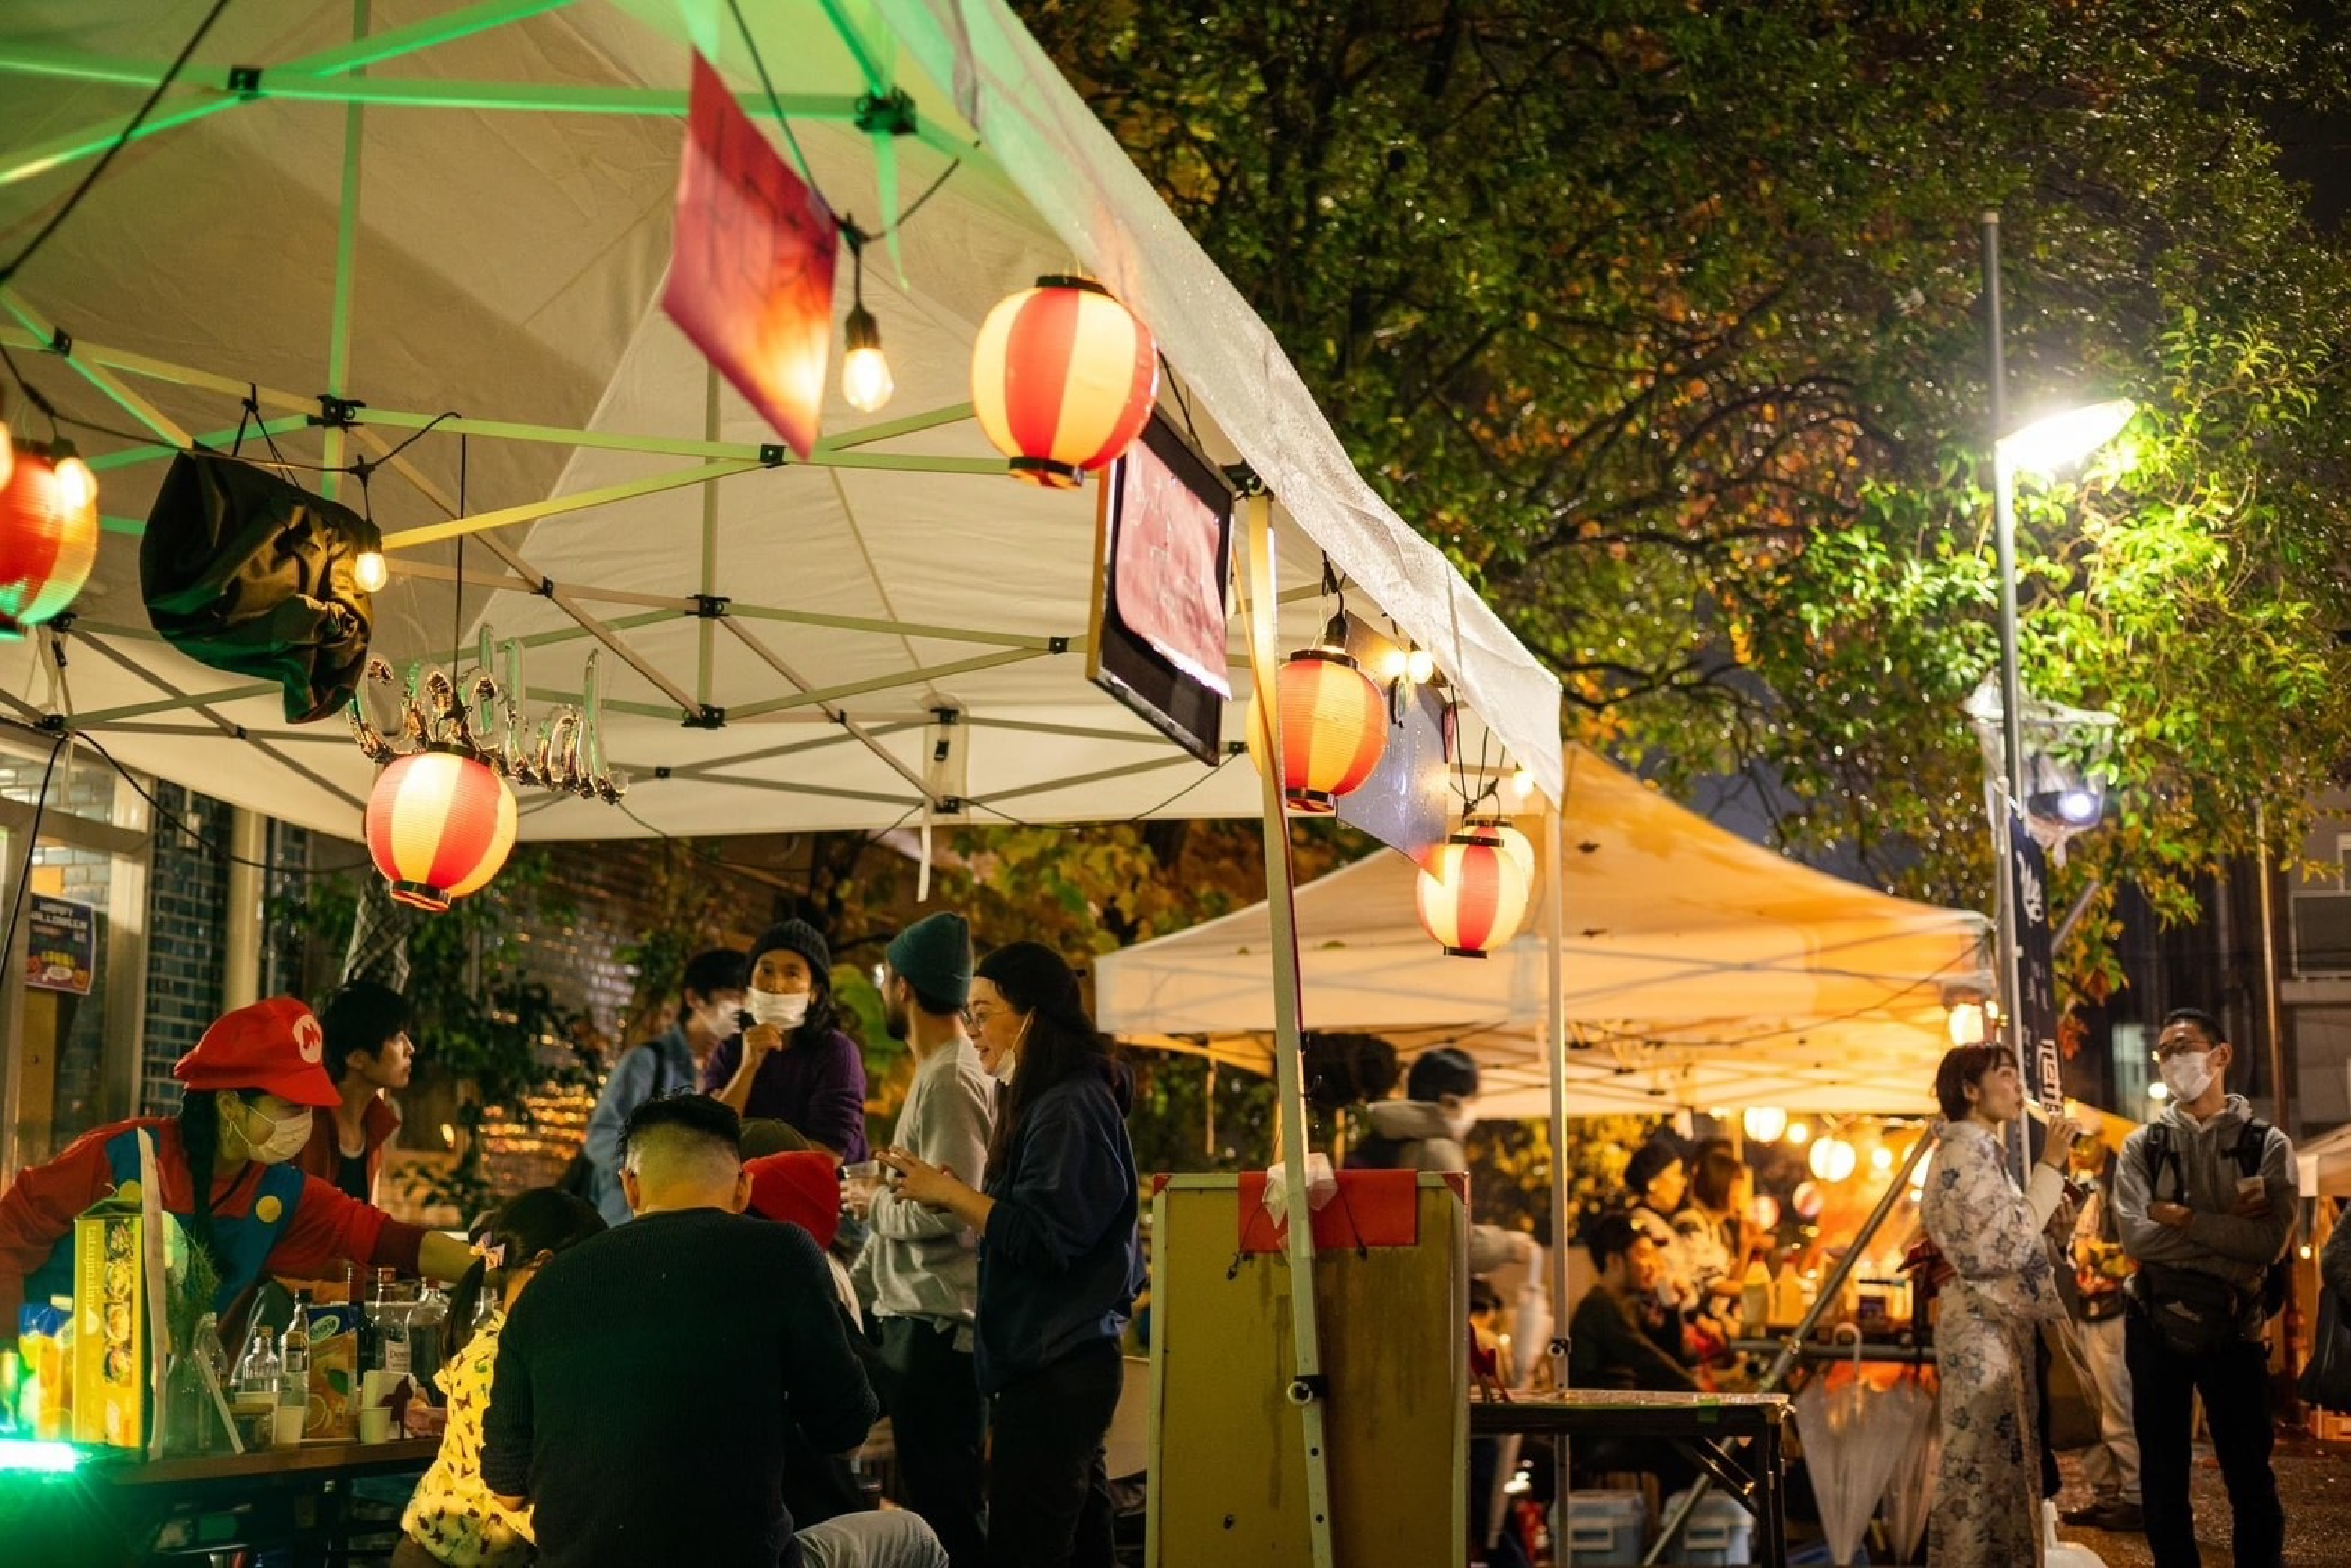
\includegraphics[width=10cm]{gazo/kumanomaturi1.pdf}
\end{figure}

さて, そこで私たちがお祭りを通してアピールするのは「過激派の巣窟なんかじゃありません」ということなのか. それは違います.空虚で中身のないレッテル貼りに対して単に「違います」「住んでいるのは普通の学生が殆どです」などと“健全さ”をアピールするのもまた空虚でしょう. 寮生が何を考え, 寮自治会がどういう理念をもってその活動を展開しているのか, 見えにくい中身の話を対面で真摯に説明することにこそ意味があります.

大事なのは, 真っ当な内容が伴っているかということだと思います. 「学ぶ権利を守るためにここまでやります」と丁寧に説明した上で, 「団体交渉を要求するとか, 昔の学生運動\index{がくせいうんどう@学生運動}みたいで過激だね」と言う方もいらっしゃいますが, 理解した上で「過激だ」と言うのは当人の自由でしょう.

レッテル貼りの材料にされようとも, 過激に見えるかもしれない抗議を続け, 中核派\index{ちゅうかくは@中核派}の学生の人権を守る,そういった中には「誰でも安心して暮らせる住居を守る」「寮を必要とする学生には住居を保障する」という, 寮自治会が貫くべき理念があります.そして,実際に祭りで説明を聞いてくださった多くの地域住民が, 警察や京大当局による一方的な権力行使に対して批判する立場に立ってくれています.

ともすれば誤解されてしまう, しかし本当は非常に重要な寮自治会の内実を, しっかりと社会に発信し, 地域の方々と顔の見える関係をつくる中で広げていこうというのが「くまのまつり」の取り組みです.

今でこそ, 盛大なお祭になった「くまのまつり」ですが, はじめからそうだったわけではありません. 寮生や寮外の協力者がお店や知人に呼びかける中で, 毎年少しずつ輪が広がっていき, このような盛大なお祭へと成長していきました. やりたいと思ったことを何でも実行に移せるのが自治寮のいいところです. 「くまのまつり」は自治会のもつ無限の可能性の一つを示す取り組みです. 入寮を検討される皆さんには入寮してもしなくてもぜひ「くまのまつり」に遊びに来てほしいと思います. 入寮してもしなくても是非一緒にお祭りやりましょう!

皆でアイデアを出し合いながらお祭を創りあげていく過程, ご近所の人と出会い語る中で新たな関係を創りあげていく過程では, かけがえのない団結\index{だんけつ@団結}が生まれます. それが熊野寮をよりよい自治寮に変えていく何よりのエネルギーなのです.




\begin{figure}[H]
  \begin{minipage}[H]{.5\textwidth}
    \centering
    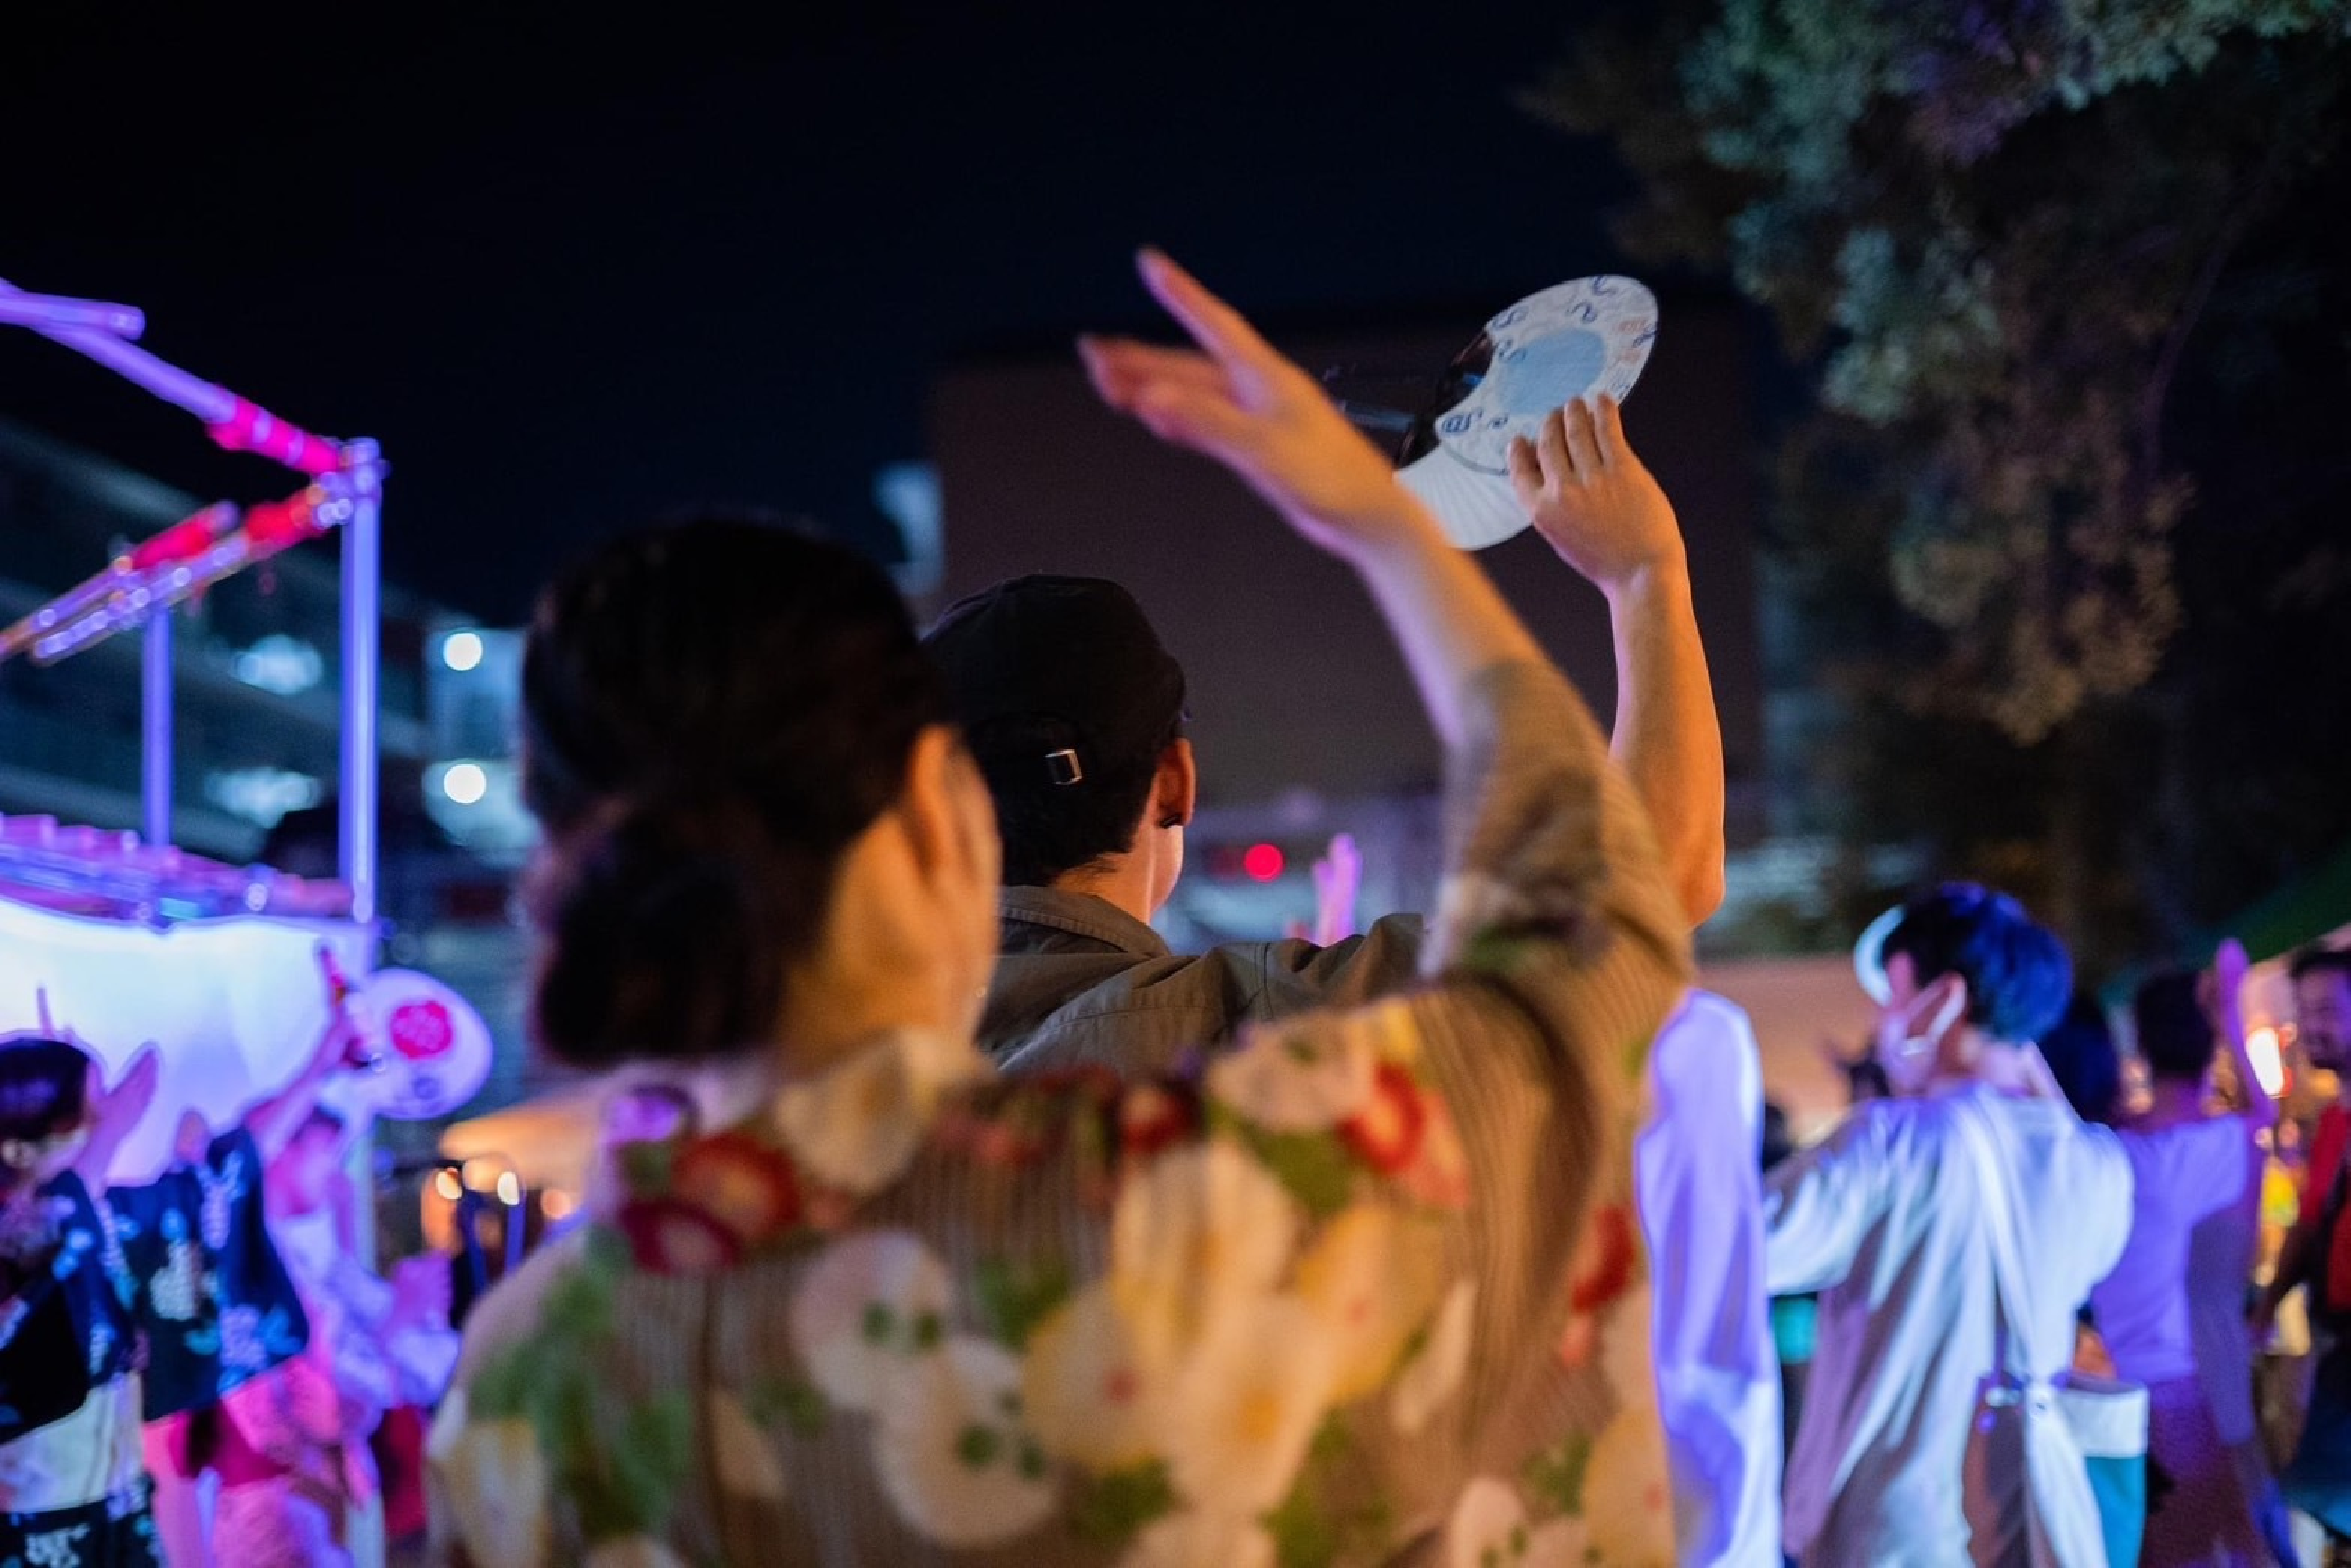
\includegraphics[width=8cm]{gazo/kumanomaturi2.pdf}
  \end{minipage}
  \begin{minipage}[H]{.5\textwidth}
    \centering
    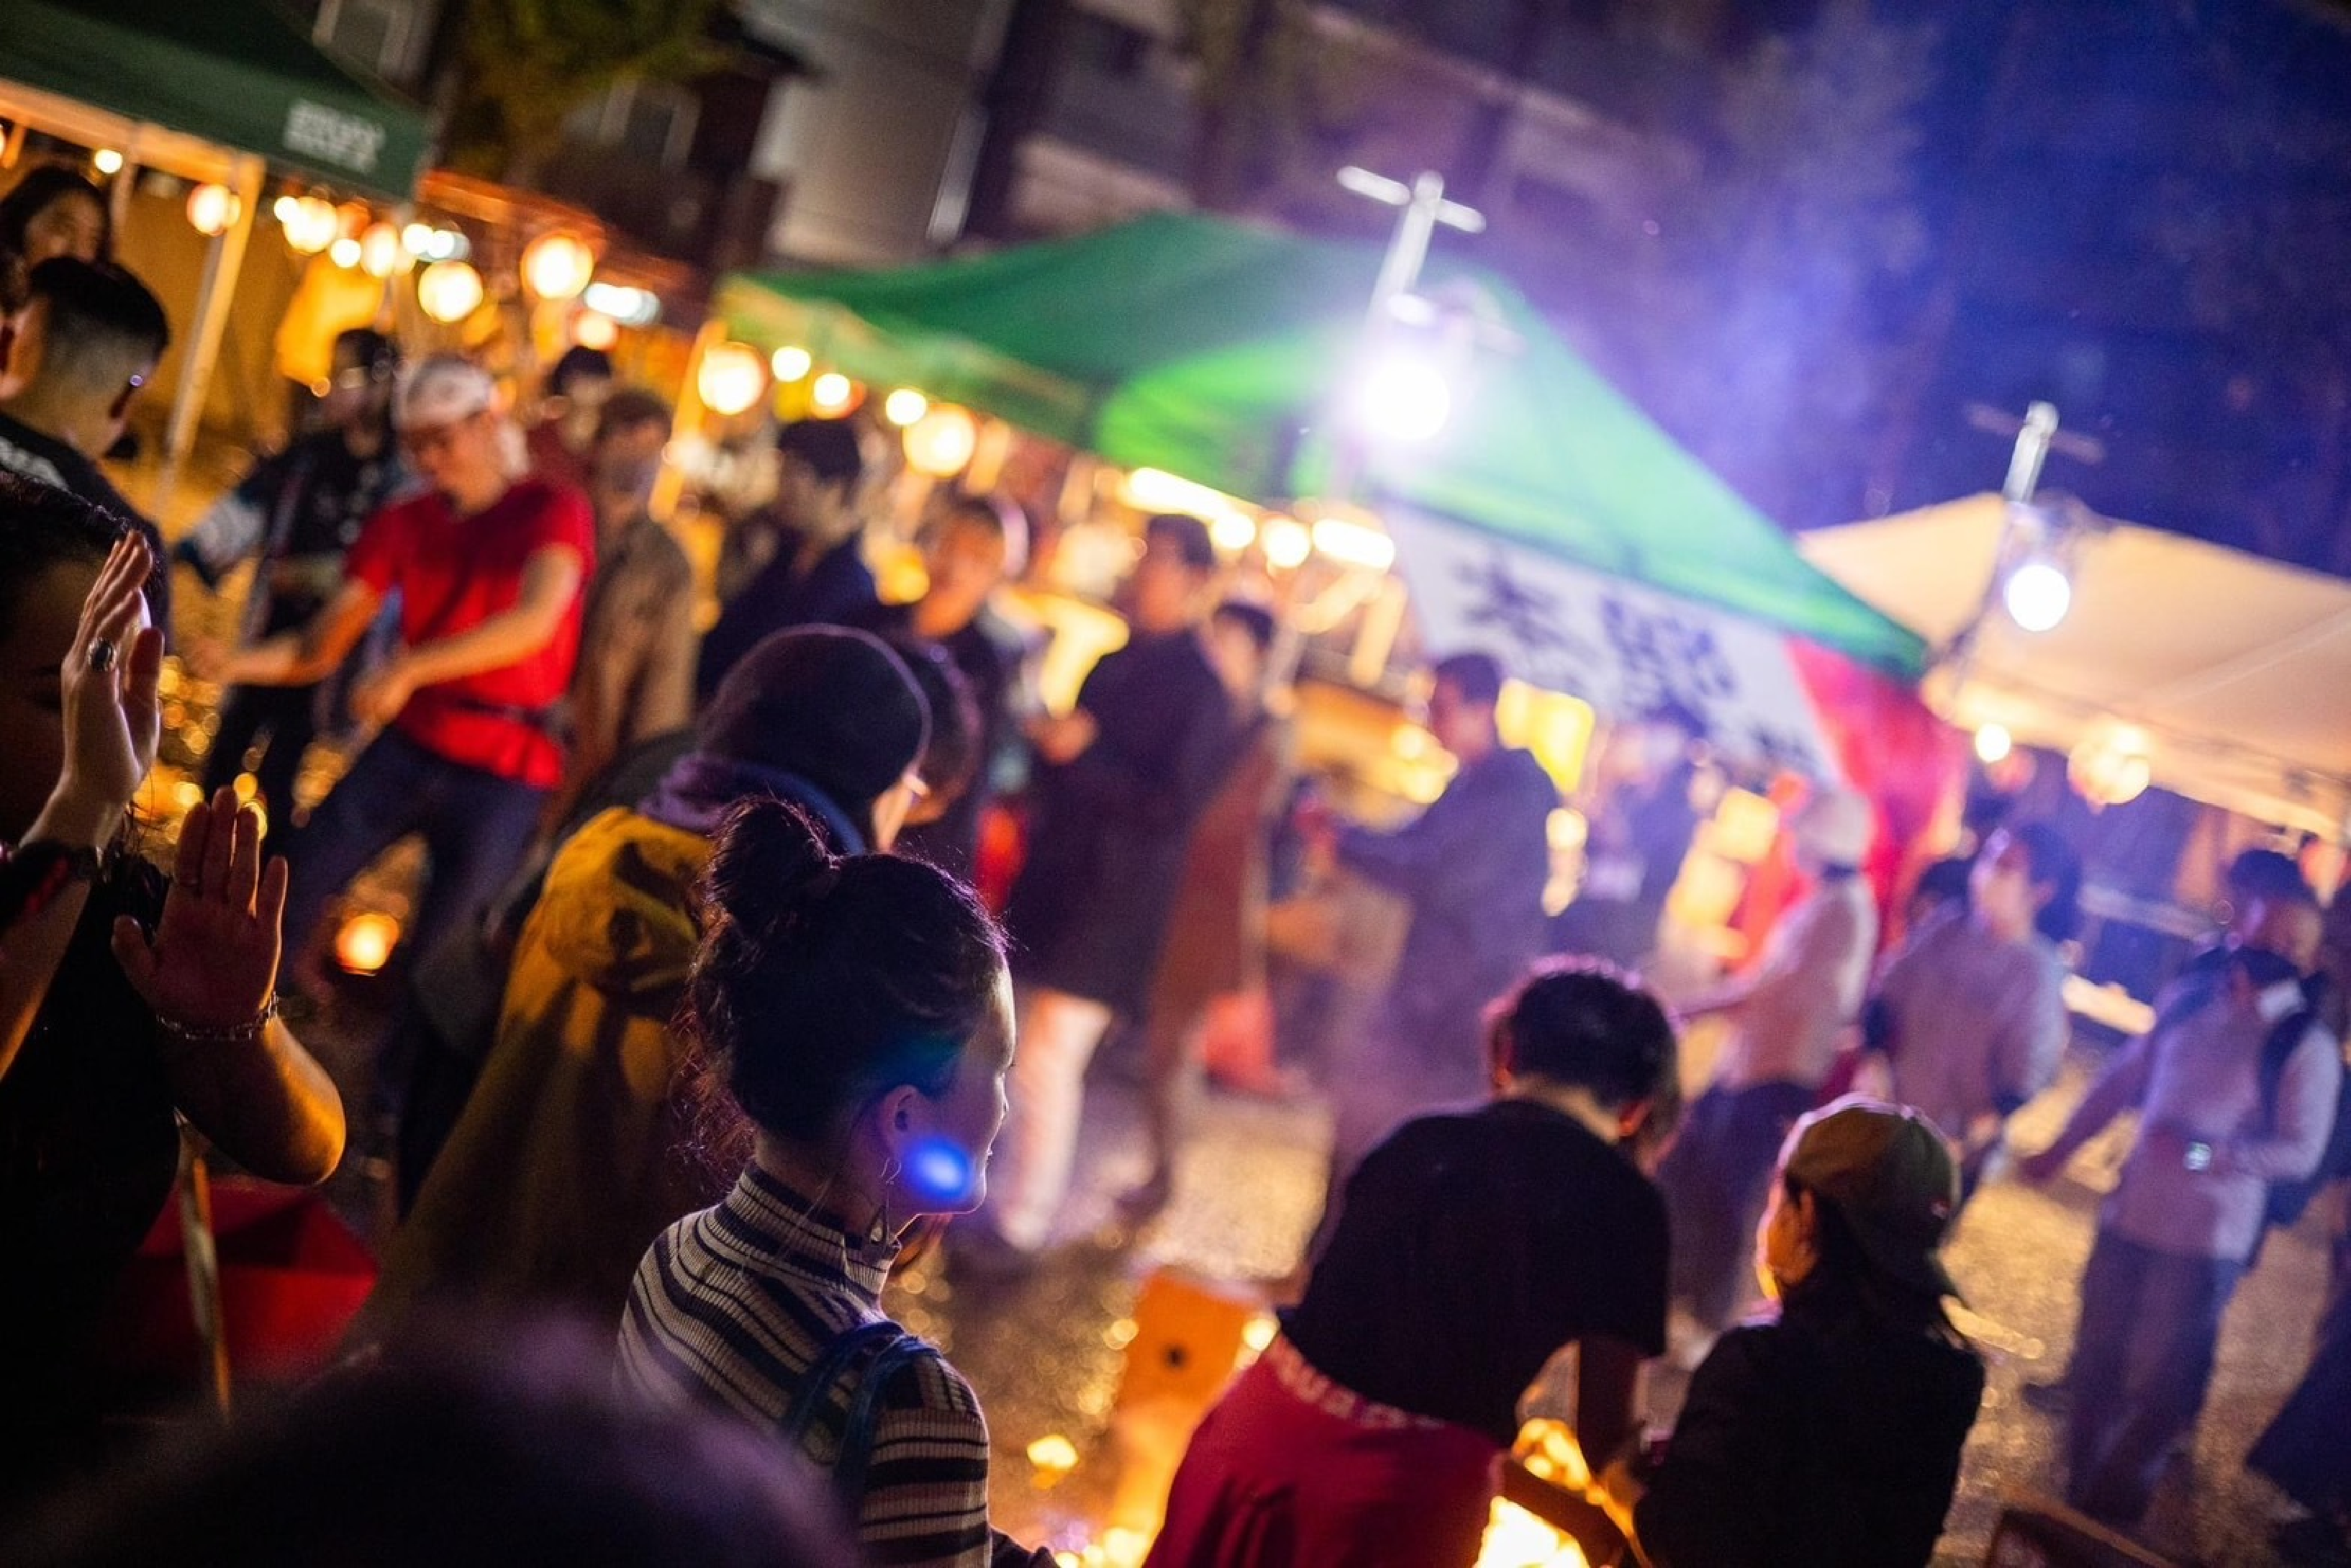
\includegraphics[width=8cm]{gazo/kumanomaturi3.pdf}
  \end{minipage}
\end{figure}



  

\chapter{寮と大学と自治}
  \section{自治とは何か}\label{sec:jiti}
\index{じち@自治!とはなにか@---とは何か|textbf}

 	みなさんこんにちは. みなさんがこれから, 入られるであろうと期待する熊野寮は「自治寮」という, 寮生で「自治」を行っている寮です. 現在でもこのような「自治」を行っている学生寮は, 全国的に見てもほとんどありません. ここでは, 熊野寮の「自治」について, 紹介したいと思います.
 	
  「自治」とは何なのでしょうか. 辞書には「自分たちのことを自ら処理すること. 特に, 地方公共団体や大学がその範囲での行政・事務を自主的に行うこと(岩波国語辞典) 」と書いてあります. すこし幅が広すぎてよくわかりませんね.

  ですが, 熊野寮の自治とは非常に単純です. それは「熊野寮のことについては熊野寮生が取り決め運営する」という, ただそれだけのことです.「そんなことわざわざ確認しなくてもあたりまえ」という人がいるかもしれません. しかしながら, 熊野寮が誇る「自治」のすばらしさは, それをとことん追求していることにあります.

  たとえば, 現在政府は学生に学生寮の入退寮権(どのような学生を寮に入れるか判断する権利) を認めていません. 従って, 全国のほとんどの大学では学生寮には大学が許可した学生のみが入寮するようになっています. では, どうして熊野寮では入退寮権を学生組織である熊野寮自治会が持っているのでしょうか. それは, 熊野寮生が「自分たちのことは自分たちで決める」と国や大学の決定に対し闘って, 勝ち取ったからです.

  また, もともと熊野寮は日本人男子学部生のみが住める寮でした. しかし現在熊野寮には, 性別も年齢も国籍も問わず, さまざまな寮生がいます. これも, 熊野寮生が「自分たちのことは自分たちで決める」「寮は全京大生に広く開かれるべきだ」といって, 1973年に取り決めたことです.

  このように, あげればきりはないのですが, 熊野寮の「自治」のすばらしさは, 「熊野寮のことについては熊野寮生が取り決め, 運営する」という自治の原則を徹底して貫いていることにあります.

	\subsection{大学自治という基本精神}

	大学自治という言葉をご存知でしょうか. 歴史を振り返ったとき, 戦時に大学は戦争協力をしたり, 国から戦争協力を強要されたりしました. \index{せんそうとがくもん@戦争と学問}その反省から, 戦後の大学人が不当な支配に屈しない教育の精神や, その証としての, 国に対する大学自治を打ち立てました. 戦後の寮自治も基本精神は同じところから始まります. 戦争協力のような国の不当な圧力に屈しないために, 学問の自由・機会均等を守るために\index{くまのりょう@熊野寮!のしゃかいてきいぎ@---の社会的意義}, 寮の自治は行われてきました. 現在でも, 熊野寮が獲得している多くの権利(上記のような入退寮権の獲得や食堂の防衛など) は, 寮生が脈々と自治を行い, 経済的に苦しい学生\index{けいざいてきこんきゅう@経済的困窮}のための熊野寮を守ってきたからこそ, こうしてあるのです.

	\subsection{自治のすばらしさ}
  \index{じち@自治!のよさ@---のよさ}

	さて, それでは自治ということについて, もう少し深く考えていきましょう. 「自治」のすばらしさとはどういう点にあるのでしょうか. それは第一に, 最も熊野寮のことを考えた運営ができるということです. 熊野寮のことは寮生が一番よく知っているのは言うまでもありません. その, 寮生が議論して導き出された運営は最も熊野寮生のことを考えた運営です.

もちろんそのためには, 寮生一人一人が寮のことに積極的に関わっていかなければ成り立ちません. 毎週行われる専門部会, それぞれの時期に活動する専門委員会, そして, 月に二回のブロック会議と年に二回の寮生大会\index{りょうせいたいかい@寮生大会}. これらの寮の諸会議を通して, 熊野寮では寮生同士が意見を活発に交わしています. 従って, これらの会議は, 自治の根幹をなす部分であり, 寮生全員の出席が義務付けられています. 「これだけ会議があると, 大変だ」という声が聞こえてきそうですが, 大したことはありません. なぜなら, 他ならぬ自らのことを決める場なのですから.\index{かいぎ@会議!のいぎ@---の意義}

  そして第二に, 自分で自らのことを決定できる喜びです. 本来はあたりまえであるはずのことですが, 今の社会ではそれすらも困難になっているのが現状です. そのような中で, 熊野寮では寮生の寮生のための寮生による運営ができるのは何よりも楽しいことです.

  第三は人と人とのつながりです. 例えば寮内で行われる季節ごとのコンパ\index{こんぱ@コンパ}や, 談話室\index{だんわしつ@談話室!でのすごしかた@---での過ごし方}などでの夜を徹しての議論や麻雀\index{まーじゃん@麻雀}に飲み会\index{おさけ@お酒}, 回生・性別・国籍\index{こくせき@国籍}を問わないその人間関係は, 自治を行っている熊野寮だからこそです.

  自分がやりたいことを周りの人に呼びかけて, 企画として実行する. 寮生の想像力に上限がない以上, 自治をしている限り熊野寮の可能性・創造性・発展性は無限大です.

  ところで, 「自分たちのことを自分たちで決める」というと, 個人主義的思考に勘違いされそうですが, そうではありません. 熊野寮は寮生みんなで運営しているものです. そこでは, 最低限のルール\index{るーる@ルール}というものがあります. それは, 相手のことを考えるということです. 例えば, 熊野寮には当番制の仕事\index{とうばん@当番|seealsopage{炊事当番, 事務当番}}があります. この仕事を誰かがサボったらどうなるでしょう. その分の仕事は別の寮生に負担となります. そのようなことは絶対に認められません.


	\subsection{寮自治の根源}

	最後に, 寮自治の大事な基本精神を.
  \index{じち@自治!のきほんせいしん@---の基本精神}
		 
  自治とは寮生みんなで行うものです. ですので, どのような立場・性別・国籍の人であろうとも, どれだけ利害が対立してようとも, あくまで対等な立場で話し合いを行うことが絶対不可欠です\index{たいとうなはなしあい@対等な話し合い}. こうした対等な話し合いで形成された信頼関係がないと, 安心して共同生活なんておくれません. このような信頼関係を築くためにも, 各寮生がお互いのことをよく知り, お互いのことを考え, 立場が異なる人とも対等に接して議論を重ねる努力をしなければいけません. これを, 徹底討論の原則といいます.\index{てっていとうろん@徹底討論}

  また, 熊野寮では何かトラブル\index{とらぶる@トラブル}が起きたときも, 押し付けや刑罰でよしとするというのではなく, 当事者が納得できるように, 最大限努力します. 寮生一人一人が, 本当に信頼できる熊野寮を目指しているからです. このような, 信頼関係が熊野寮自治の根源なのです.

  長くなりましたが, これで自治の紹介は終わりです. みなさん納得していただけたでしょうか. まだ「?」というところもあるかもしれませんが, それは入寮されてからということにしておきます. 寮はみんなが作っていくもの. たくさんの信頼できる仲間に囲まれた, 心躍るような寮生活を, 熊野寮でともに過ごそうではないですか. みなさんの入寮を心よりお待ちしております.

  \clearpage
  \section{大学当局との確約・団体交渉}\label{sec:kakuyaku}
	熊野寮自治会が大学当局と結んでいる確約と団体交渉について説明します.\index{かくやく@確約|textbf}\index{だんたいこうしょう@団体交渉|textbf}

	\begin{shadebox}
	\textbf{言葉の解説:大学当局} \\
	「京都大学」には学生個人や多くの学部・寮自治会などの組織も含まれます. それら学生側と区別して大学運営の中枢である事務本部や各担当部署を指す言葉です. 「我々大学当局としては...」というように, 京都大学では職員や教員にも一般的に使われている言葉です.\index{だいがくとうきょく@大学当局|textbf}
	\end{shadebox}

		\subsection{確約}
		確約とは熊野寮自治会と京都大学当局との間に取り交わされた約束です. 実際に居住している当事者である寮生の意見を無視して当局が一方的な決定を下すことを防ぎ, 当局と寮自治会が対等に協議できるようにするために, 当局側の権力行使に制限をかけるものです.

		\subsection{「対等」な話し合い}
 		前項で「当局と寮自治会が対等に協議できるように」と述べましたが, 法的に管理権を有する当局と学生の間には大きな権力差があるということが前提になっています. だからこそ, その力の差を可能な限り埋め合わせ, 可能な限り対等な話し合いによって学生のよりよい福利厚生を実現しようとしているのです.

		例えば, 寮生は交渉で発言する際にも当局に対して名乗ることはありません. 所属を特定されて個人単位で弾圧される危険性があるからです. 京大では近年もアカデミックハラスメント\index{あかはら@アカハラ}が起きています. 自分の「家」について当局と意見が違っただけで, 学業面で不当な扱いを受けることがあってはなりません.もちろん, そもそも組織間の交渉なので, 寮自治会の立場を述べるのであれば, 個人が名乗る必要がないということでもあります.\index{くまのりょう@熊野寮!じちかい@---自治会}

		\subsection{確約の引き継ぎ}
		確約書は厚生担当副学長の署名によって結ばれており, 形式的には副学長個人の寮に対する約束となっています. しかし, 「熊野寮自治会と京都大学の基本確約」(\pageref{page:確約}頁参照)とあるように, 本来的に確約は組織間の約束です. 例えば担当者(任期2年の副学長)が交代したからといって, 大学と自治会の約束がいちいち白紙に戻っては困ります. その為に, 副学長が交代しても引継ぎが自動的に, 確実になされるよう, 「次期以降の学生担当理事, 厚生補導担当副学長に引継ぐ. 」という条文が定められています.

		ちなみに現在は, 当局の責任者として國府寛司副学長が寮自治会と確約を結んでいます.

		\subsection{団体交渉}
		当事者(寮生は勿論, 今後入寮しうる京大生, その他関係者など誰でも) がすべて自由に参加できる, 公開の交渉形態です. 確約の引継ぎや, 新寮の建設など寮にとって重大な事案についての団体交渉が, 学内の大教室や寮食堂などで開かれてきました.

		例えば対照的に, 少人数の交渉形態, つまり寮自治会の代表者数名だけが参加できる協議の場というのはどうでしょうか. 経済的に苦しくてアルバイトで忙しいため自治会の交渉事に中心的に参加できていない者や, 入寮したばかりで確約などの詳しい知識が無かったりする者など, 「自分の家のことが協議される場に参加したい」という思いは皆同じです. すべての当事者(特に居住している寮生) には協議・意思決定の場に参加する権利があると考え, この形態で交渉することが条文でも定められています. 団体交渉という形態を拒否すること自体も確約違反なのです.

		\label{page:確約}

		\begin{tcolorbox}[colback=white, colbacktitle=gray!30!white, coltitle=black, title=熊野寮自治会と京都大学の基本確約,breakable]

		熊野寮自治会と京都大学は, 2004年3月31日に結ばれた, 両者の確約書に則り, 以下の内容に合意する. 両者は熊野寮が京都大学学生全体に開かれたものであることを確認し, その一層の充実のため誠実にこの確約内容を履行するものとする. 両者は学生の居住する熊野寮の運営に関しては, 当事者であり主体的にその責任を果たす学生の自治によることが最良であることを確認し, この認識を基礎にこの確約を結ぶものである.本確約は文書としては二通作成し, 両者が一部ずつ所持するものとする.

		\begin{enumerate}
		\renewcommand{\labelenumi}{(\arabic{enumi})}
		\item 京都大学は福利厚生施設としての熊野寮を設置し, \index{ふくりこうせい@福利厚生}その施設を維持・管理する. 京都大学は熊野寮の一層の充実に努めるものとする.
		\item 京都大学は, 熊野寮の日常的運営が熊野寮自治会によることを確認し, 熊野寮自治会\index{くまのりょう@熊野寮!じちかい@---自治会}はその運営を誠実に行うよう努力する.
		\item 京都大学は, 熊野寮の改廃や新寮および新規寮建設, 熊野寮に関わる人員配置, またその他熊野寮に重大な影響を与え得る事案に関しては, 公開の場で熊野寮自治会と団体交渉を行い, 合意の上決定する.\index{だんたいこうしょう@団体交渉} 加えて, 熊野寮自治会と京都大学は, 一方が提示した議題に真摯に取り組むものとする.
		\item 熊野寮自治会または京都大学は, 両者の協議の場において, 何らかの条件を付そうとする場合には, 相手側の同意を得るものとする.
		\item 熊野寮自治会または京都大学は, 熊野寮に重大な影響を与えうる事案について何らかの計画を構想した段階で, 相手方にその内容を報告するものとする.
		\end{enumerate}

		\flushright{京都大学副学長 \\ 熊野寮自治会}

		\end{tcolorbox}
		

		\begin{tcolorbox}[colback=white, colbacktitle=gray!30!white, coltitle=black, title=確約,breakable]

		%\centerline{\bf 確約}

		上記の「熊野寮自治会と京都大学の基本確約」ならびに2010年12月17日の赤松副学長(当時) による「確約書」を基礎にして, 以下の内容を遵守する.

		\begin{enumerate}
 		\renewcommand{\labelenumi}{(\Alph{enumi})}
		\item 熊野寮食堂の機能の維持・向上について
			\begin{enumerate}
			\renewcommand{\labelenumii}{(\arabic{enumii})}
			\item 過去に熊野寮食堂の食堂労働者を削減した事実を認める.\index{ちゅうぼういん@厨房員}
			\item 現在の熊野寮食堂の食堂労働者の置かれている労働環境が劣悪であることを認め, その改善に努める.
			\item 熊野寮食堂において, 食中毒が発生したり, 感染症が持ち込まれたりしても, これを理由とした食堂廃止は行わない. また保健所の指摘を理由とした食堂廃止も行わない.
			\end{enumerate}
		\item 京都大学熊野寮食堂運営会( 以下, 「食堂運営会」とする) について
			\begin{enumerate}
			\renewcommand{\labelenumii}{(\arabic{enumii})}
			\item 2013年6月21日に改正された「京都大学熊野寮食堂運営会会則」ならびに2014年6月20日に改正された「京都大学熊野寮食堂運営会就業規則」を遵守する.
			\item 食堂運営会雇用調理員に対する一定の雇用責任を認め, 労働災害発生時の補償責任を負う.
			\end{enumerate}
\item 寮内労働者について
			\begin{enumerate}
			\renewcommand{\labelenumii}{(\arabic{enumii})}
			\item 寮内労働者の雇用形態について本来ならば全員大学雇いが望ましいことを認め, その労働環境・労働条件に関しては改善に努める.
			\item 恒常的業務に従事する寮内労働者が退職となった場合には, 後任を補充する. この後任補充の際, 雇用形態や労働条件などの, 労働に関わるすべての条件を, 前任者と同等もしくはそれ以上で確保する.
			\end{enumerate}
		\item 寮の生活環境の向上について
			\begin{enumerate}
			\renewcommand{\labelenumii}{(\arabic{enumii})}
			\item 寮自治会から生活環境に関する要求があった場合には, その要求された箇所について調査を行い, そのための工事や改修について検討する. また, その検討結果を速やかに寮自治会に報告する.
			\end{enumerate}
		\item 熊野寮に対する家宅捜索などについて
			\begin{enumerate}
			\renewcommand{\labelenumii}{(\arabic{enumii})}
			\item 熊野寮に対する家宅捜索の立会いの方法について, 熊野寮自治会からの要求があった場合には, 熊野寮自治会と協議する.
			\item 熊野寮に対する家宅捜索において, 寮自治会への令状不提示, 過剰警備(玄関前等の占拠) , 抗議する寮生や掲示物のビデオ・写真撮影など自治や人権を侵害する行為が行われた場合には, その場で抗議する.
			\item 熊野寮に対する家宅捜索\index{がさ@ガサ}が不当であるかどうかを検討し, 寮自治会に対して, その検討内容を明らかにする. 不当であると判断した場合には, 速やかに抗議する.
			\item 熊野寮自治会から「外部団体により不当な扱いを受けたので抗議してほしい」という要求があった場合, 大学職員がその不当な扱いを現認したか否かにかかわらず, 抗議の是非を検討する. また熊野寮自治会からの要求があった場合には, その不当な扱いについて, 熊野寮自治会と協議する.
			\end{enumerate}
		\item 桂キャンパスの利用について\index{かつらきゃんぱす@桂キャンパス}
			\begin{enumerate}
			\renewcommand{\labelenumii}{(\arabic{enumii})}
			\item 熊野寮生をはじめとする学生の桂キャンパスへの通学において, 不便とならないように努める.
			\item 桂キャンパス周辺に新規寮を建設することを検討する.
			\end{enumerate}
		\item 寮自治会と国立大学法人京都大学の関係性について
			\begin{enumerate}
			\renewcommand{\labelenumii}{(\arabic{enumii})}
			\item 中期計画, 年度計画を文部科学省に提出する前に, 寮に対してどのような影響があるのかを寮自治会に対して提示・説明し, 寮自治会からの要求があった場合には, 内容を変更することが可能な協議の場を持つ.
			\item 国立大学法人運営費交付金など大学法人の収入減少を理由とする寮関係予算の削減を行う場合, その重大性などに関する寮自治会との真摯な議論を経て, 寮自治会と合意するものとする.
			\end{enumerate}
		\item 団交--確約体制ならびに確約の引継ぎについて
			\begin{enumerate}
			\renewcommand{\labelenumii}{(\arabic{enumii})}
			\item 学生担当理事, 厚生補導担当副学長は, 熊野寮自治会との間において, 団交--確約体制を維持する.
			\item 学生担当理事, 厚生補導担当副学長は, 「熊野寮自治会と京都大学の基本確約」ならびに本確約を, 次期以降の学生担当理事, 厚生補導担当副学長に引継ぐ.
			\end{enumerate}
		\end{enumerate}

		\end{tcolorbox}
  \clearpage
  \section{厨房労働者の雇用形態と人件費負担について}\label{sec:tyuboin}

	現在, 熊野寮食堂の厨房に勤務する5名の栄養士・調理員のうち, 調理員2名については大学雇用ではなく, 寮生が人件費と労働保険料を負担している. 我々はこの現状の問題性を見失ってはならない.\index{しょくどう@食堂}

		\subsection{「受益者負担の原則」とそれを否定する熊野寮の立場}\index{じゅえきしゃふたんのげんそくのひてい@「受益者負担の原則」の否定}

	「受益者負担の原則」とは「利益を得ている人」が金を払えという考え方である. これは60年代から国が押し出してきたものである. 教育について言えば, 「教育を受ければ将来良い職について金持ちになるから, 将来の自分への投資として金を払え」というような論法となる.

	それに対して, 社会の維持発展のために教育は必要であるという事実から, 社会に必要なものは社会全体で保障すべきであるという考え方がある. 社会全体が利益を得ているから社会全体で金を賄うというものである.
	つまり「受益者負担の原則」を否定する考え方である. 熊野寮自治会はこの立場で運動し, 国・当局との攻防を繰り広げて今にいたる.

	こう考えれば, 調理員の人件費についても本来公費で賄われるべきであり, つまり京都大学が調理員の雇用を保障すべきである.\index{ちゅうぼういん@厨房員}

	歴史を見れば, 寮自治会が運動した結果, 1969年7月以降, 調理員全員が京都大学に公務員として雇用されていた. 大学当局すらも, 国策である「受益者負担の原則」に反対する立場に立たせたのである.


		\subsection{食堂運営会とは}

		食堂運営会(正式名称:京都大学熊野寮食堂運営会) とは, 熊野寮食堂の厨房に勤務する5名の栄養士・調理員のうち, 寮生が人件費と労働保険料を負担している調理員2名を雇用し, その労働条件を維持・改善するためにつくられた組織である. 会長には京都大学副学長が着任し, 全寮生が会員ということになっている.

		60年代の時点では, 熊野寮食堂の厨房調理員は全員公務員(つまり大学が雇用主) だったが, 1979年12月, 大学側が国が推し進める受益者負担の原則や新々寮四条件\footnote{文科省の認める学寮の条件(新々寮4条件),
\begin{enumerate}
\item 全部屋個室
\item 食堂なし(集会スペースをつくらない)
\item 負担区分全面適用(居住に関しては個人と大学の間の契約関係に依拠)
\item 入退寮選考権は大学持ち(同上)
\end{enumerate}}
公務員削減政策を理由に, 調理員をそれまでと同じ条件では(つまり公務員としては)雇わないことを一方的に宣言した. それ以降4度の臨時職員の後任不補充が行われ, 抗議の甲斐もなく, 結果として寮生側は自分たちで人件費を払ってパート(時間雇用) 調理員2名を雇うことになったのである.

		さらに, 大学との間で誰がそのパート調理員の労働関係上の雇用主となるべきかをめぐって見解が合わず\footnote{寮生側は学生と職員の福利厚生に責任のある大学に全面的な雇用責任があるとし, 大学側は実質的に人件費を支払っている寮生にあるとした. }, 交渉が長期化した. その結果, 雇用主が不明確という理由で寮生負担パート調理員は長いこと労働保険にも正式に加入することができなかった. 労働保険(雇用保険・労災保険) への加入は全ての労働者に与えられた権利であるが, 寮生負担パート調理員はその労働者にとっての基本的な権利すら許されないまま放置されていたのである.

		そこでこの人権侵害的な状況を改善するため, 寮生側から大学に対し, 「食堂運営会」を設立し, その組織を寮生負担パート調理員の雇用主とすることを提案したのである. 取り決めとしては, 「人件費, 保険料は今までどおり寮生が払うこと」「大学側は労災時の補償責任を負うこと. また, 大学副学長は会長に就任すること」という形で, 大学と寮生が運営会雇用調理員の雇用責任を折半して負う形であった. この提案は認められ, 2005年4月から食堂運営会は発足し, 食堂運営会雇用調理員(旧寮生負担パート) は労働保険に加入することができた. 確約によると, 寮生は食堂運営会雇用調理員(旧寮生負担パート) 2名の人件費・保険料を負担し, 大学側は労働災害発生時の補償責任を負うことになっている.

		食堂運営会の今後の課題は, 食堂運営会雇用調理員さんの現在の労働条件を維持し, 働きやすい労働環境を守っていくことである. そのため, 日頃の調理員さんとのコミュニケーションはもちろん, 年2回開かれる食堂運営会総会や毎年の会長指名(会長の任期は1年) , 副学長の代替わり毎に行なう団交・確約を確実にこなさなければならない. これよりもう一段階進んだ課題としては, 調理員さんに対する人件費・保険料支払いも含む完全な雇用責任を大学に認めさせ, 大学を雇用主にすること(つまり労働条件の「正常化」) がある.

		
		このような調理員の雇用状態に代表される受益者負担の考えに基づく大学の方針は、低価で生活できる学寮の意義を放棄するものである。またこの雇用問題によって引き起こされる厨房の不安定さは食堂の維持の困難にもつながる。食堂は寮食を喫食する場であると同時に、様々な人との交流、議論の場であり、自治に欠かせない空間である。実際、食堂が大学当局によって廃止され、その後に管理寮・廃寮化に追い込まれた自治寮もある。(2011年3月の富山大学新樹寮食堂の廃止→富山大新樹寮 2011 年管理寮化など。)寮生の共同空間を破壊することで, 寮生間の自由なコミュニケーションを否定し、個々人を分断管理 (集団として行動できないように) する思惑が働いているのだ。全国の自治寮はこの問題に対し、経済的弱者を切り捨てた上での徹底管理を狙ったものであるとして長年抗議してきた。つまり、食堂は自治寮防衛の最前線の一つであると言える。そのため雇用問題は熊野寮が自治寮であり続けるためにも、向き合わなければならない問題なのだ。

		\begin{shadebox}
      \textbf{学寮不要の文部省方針} \\
      1971年の中央教育審議会答申で, 文部省は学寮を「紛争の根源地」と断定, その教育的意義を否定した. これに基づいて多くの学寮で, 水光熱費の徴収や入退寮権を大学当局が把握していった. 大阪大学, 岡山大学などでは, 大学当局が反対する寮生を機動隊の力を借りて抑圧し, 自治寮の廃寮化を進めていった.
			\index{がくりょう@学寮|seealsopage{吉田寮}}
      
      \tatespace
      自治寮は, かつては全国にあったが, 次々と廃寮化, 管理化されている.
      \begin{itemize}
        \item 東大駒場寮2001年廃寮化
        \item 東北大有朋寮2003年管理寮化
        \item 富山大新樹寮2011年管理寮化
        \item 東京芸大石神井寮2014年廃寮化
    \item 金沢大学泉学寮2023年廃寮化
      \end{itemize}
      など
  \end{shadebox}

  \clearpage
  
\section{学生処分問題と熊野寮自治会の対応}
\label{sec:shobun}
\bunsekisha{文責}{対処分戦略推進局}
\index{がくせいしょぶん@学生処分|textbf}


高校でも生徒が「問題」行動を起こした時に、反省文を書かされたり、停学にさせられるなどの処分が行われることがありますが、京大でも似たような措置が不当かつ恣意的に行われ、学生の自由と人権が抑圧されているという現状があります。近年の京大では吉田寮問題や立て看問題(後述)など、大学当局からの学生への抑圧が強まっており、徐々に自由な雰囲気を失いつつあります。しかし京大には、今の自由を守ろう、いや、今よりもっと自由な京大を作ろう、と考え行動している学生がまだまだたくさんいます\index{じゆうのがくふう@自由の学風}。処分はそうした「問題」行動を起こす学生への脅しとして使われてしまっているのです。ここでは、熊野寮の要求書提出時に職員に抗議した3名の寮生が無期停学処分にされたこと、京大の二次試験の会場に像を設置した寮生1名が\ruby{譴責}{けん|せき}処分にされたこと、時計台占拠というイベントに参加したとして8名の学生が処分されたことの3つの事例を紹介し、何が問題なのか、今まで寮としてどんな対応をしてきたか、これからどうするべきか、ということについて書きたいと思います。

\begin{shadebox}
{\large\textbf{出る順! 処分問題単語帳}}
\begin{description}
    \item[処分(正式には「学生懲戒処分」)] 当局が「問題だ」と考える学生に当局が与える罰。京都大学学生懲戒規定(\url{https://www.kyoto-u.ac.jp/uni_int/kitei/reiki_honbun/w002RG00000283.html})に手続きの定めがある。要は、当局の都合の悪い学生を屈服されるための最終手段。 処分の軽重は学部の教授会が上申するが、最終的には当局が決定する。
    \item[当局(「大学当局」「京大当局」とも)] 法律上京都大学で一番偉い「役員会」(「理事会」と言われることも多い)を中心とした大学執行部やその意向を受けて学生と対峙することになる職員全般を指す。単に「京大」とか「京都大学」だと、教授会のことを指すのか、役員会のことを指すのか、僕ら学生のことを指すのか、それともそうしたものを全部ひっくるめているのか、分からないので「当局」は便利な言葉だ。処分問題に限らず京大内では頻出語なので絶対に憶えておこう。\index{だいがくとうきょく@大学当局}
    \item[教授会] 	各学部(学科)の教員で構成される会議体で、昔はとっても偉くて学部ごとの独立が強かった(学部自治)けど、今は役員会の方が偉くなってしまった。
    \item[学生自治会] 学部や寮などに組織されている学生全員加盟制の自治会。学生のために自分たちで動いたり、当局と交渉したりしている。学生自治会がない学部や寮もある。熊野寮自治会は学生自治会の一つだ。\index{がくせいじちかい@学生自治会}
    \item[停学] 大学構内に入れず、当然授業も受けれず、図書館も使えないのに授業料は満額取られてしまうというヒドい処分。有期停学(6月未満)と無期停学がある。無期停学よりヒドい処分としては、京大に在籍したという記録自体が抹消され、学生の身分も剥奪される「放学処分」がある。\index{ていがく@停学}
    \item[\ruby{譴責}{けん|せき}] 学部長に怒られるという処分。停学よりは軽いが、実質的には「次やれば停学」を言い渡されるようなもので学生の威圧には十分だ。
\end{description}
\end{shadebox}


\subsection{寮生に暴行を振るう職員に抗議しただけで無期停学!?}
熊野寮自治会は自治会として大学当局に要求することを要求書\index{ようきゅうしょ@要求書}にまとめて、当局の「厚生課」と呼ばれる窓口に提出することあります。事件が起こったのは2018年10月の要求書提出のときです。一人の寮生(以下Aとします)が職員に取り囲まれ、暴行を受けました。Aさんが覆面をしていたため、当局はこの行為を「不審者対応」であると称しています。これに対して、提出に参加していた3名の寮生が、職員とAさんの間に割って入り、職員に抗議しました。この抗議が「業務の妨害」とみなされ、2019年9月に3名に対して無期停学処分が下されました。このうち1名はいまだに停学が続いています。


\newpage

\subsection{オルガ像を設置して譴責処分!?}

\begin{wrapfigure}{r}{8zw}
    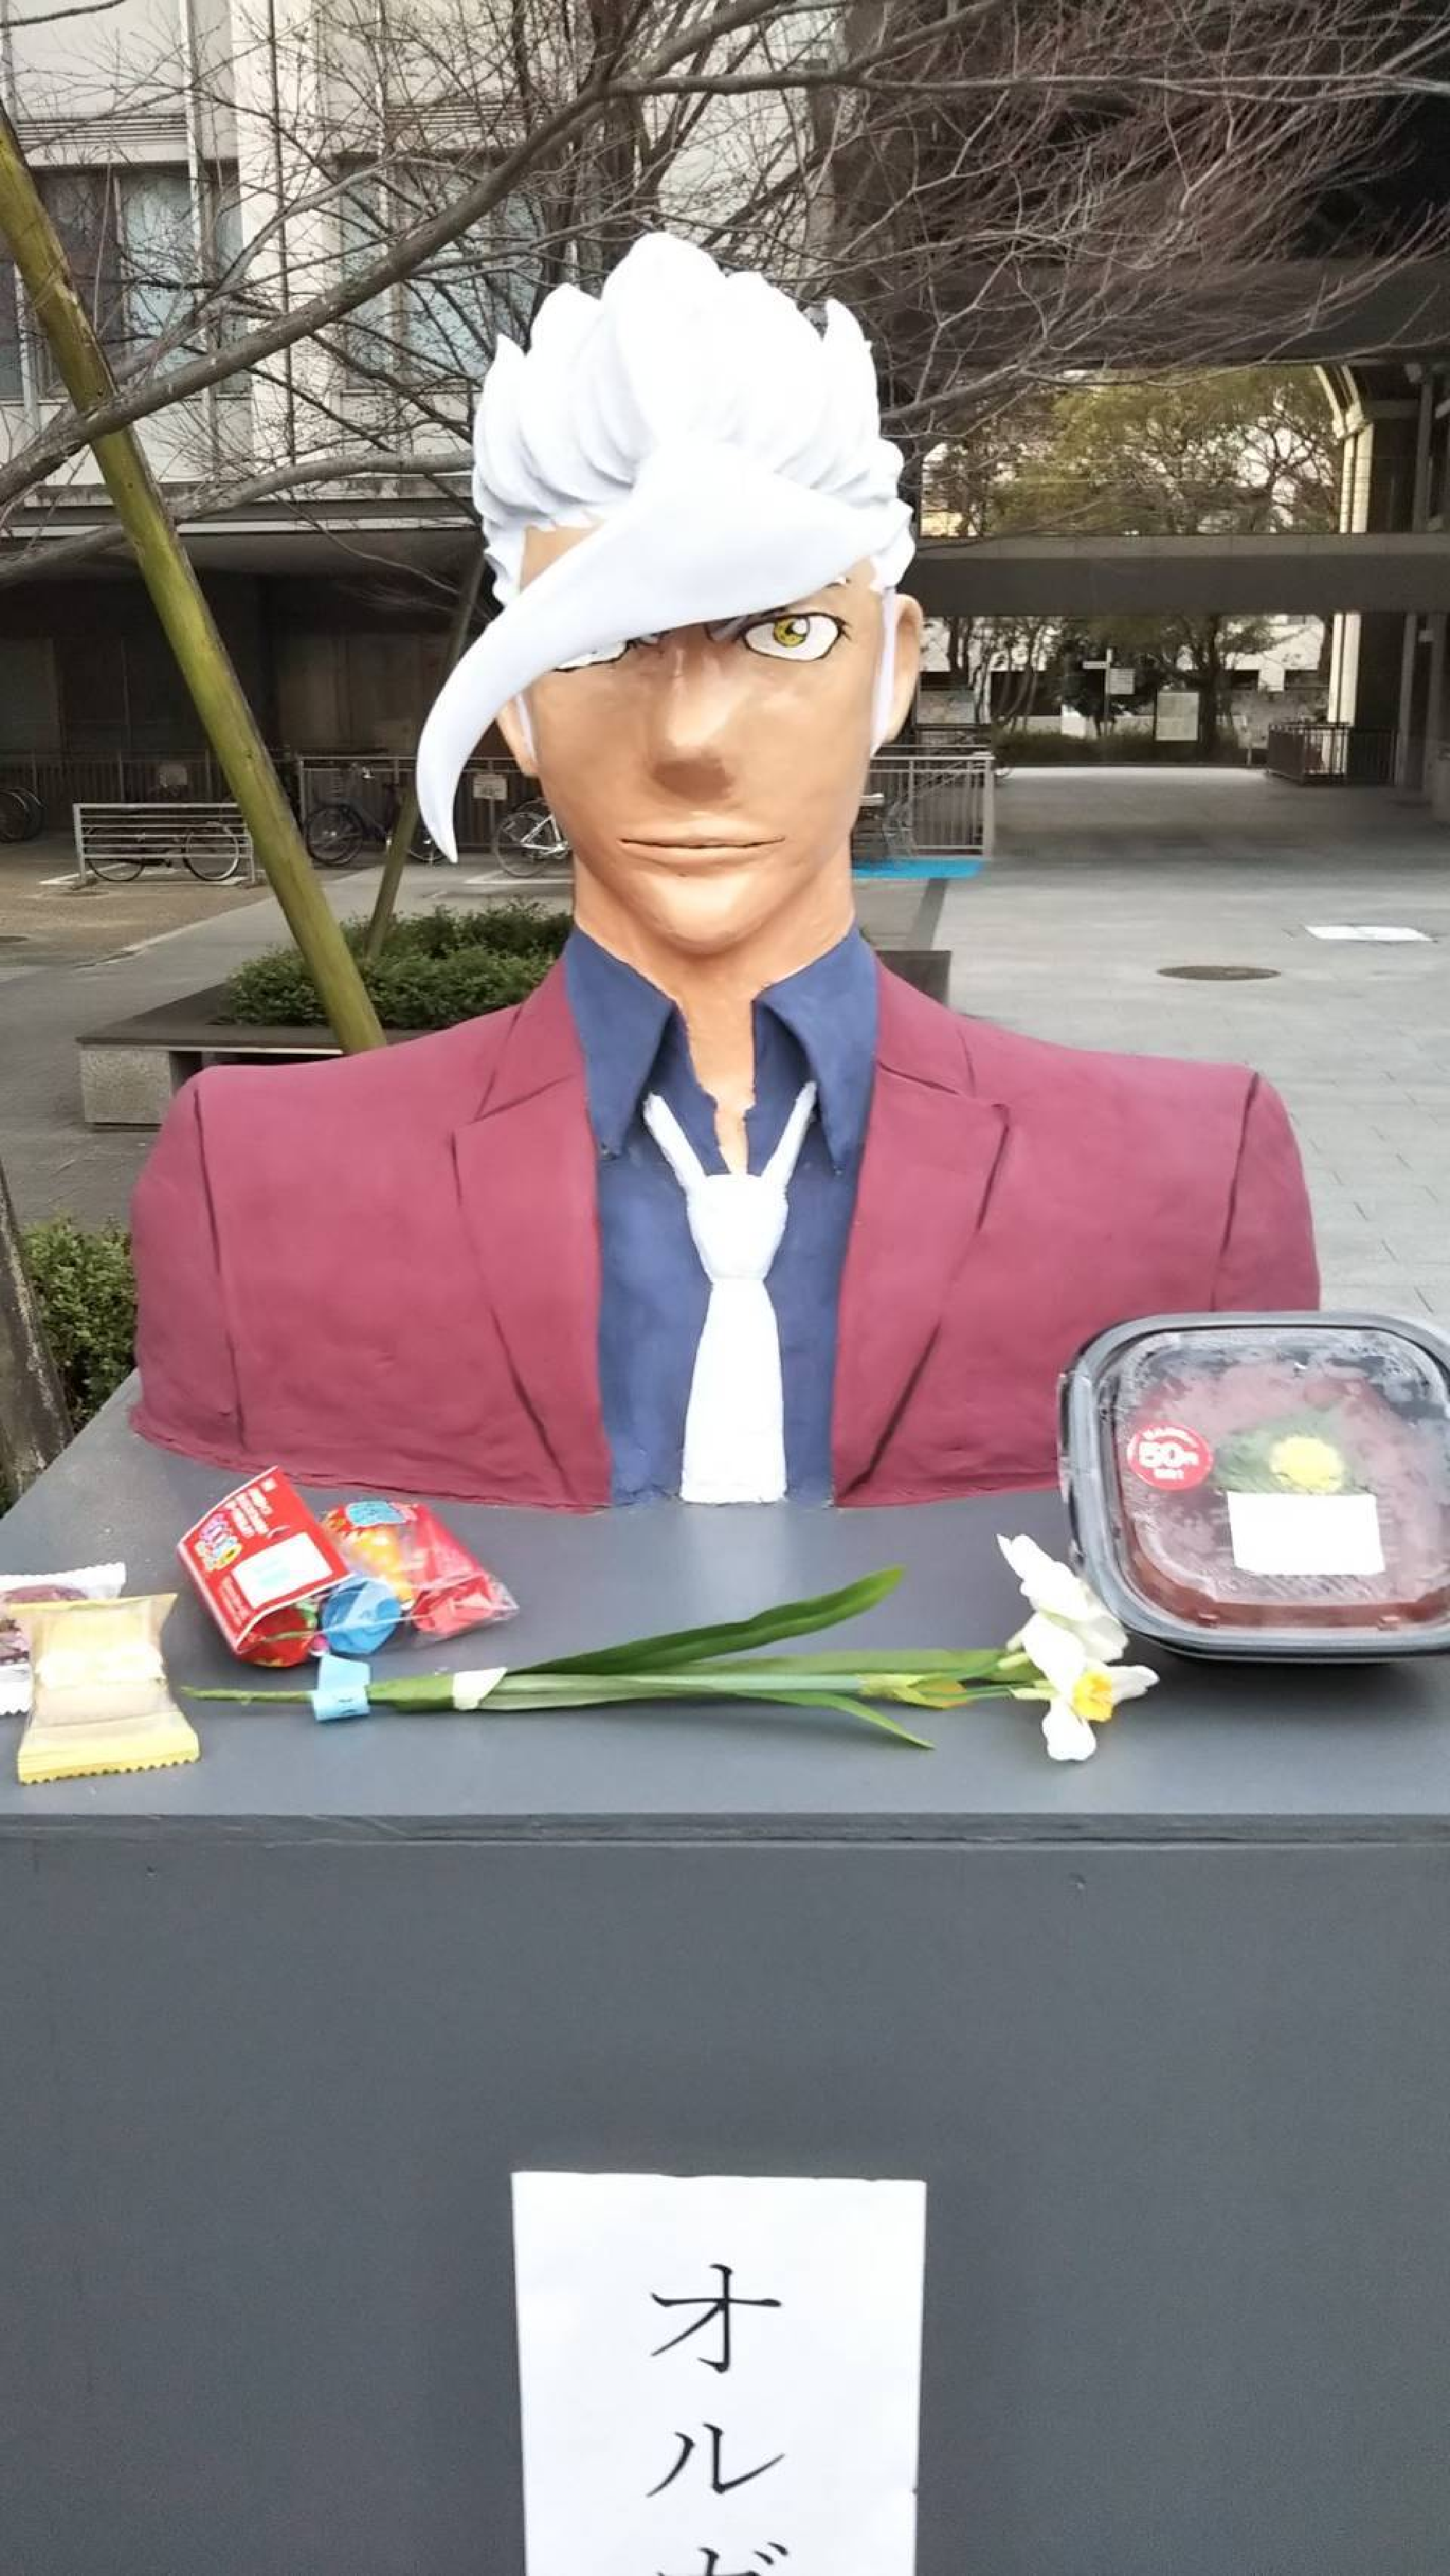
\includegraphics[width=8zw]{gazo/oruga.pdf}
    \captionsetup{labelformat=empty,labelsep=none}
    \caption{オルガ像}
\end{wrapfigure}

\index{おるがぞう@オルガ像}
読んでいる人の多くが京大の二次試験でパンフを受け取ったと思います。京大の二次試験は様々な学生が立て看や像を立てたり、入寮パンフを配ったり、受験生と麻雀をしたりと、構内は受験生激励で非常ににぎやかになります(もちろん試験時間中は静かです)。2019年の入試会場での『機動戦士ガンダム 鉄血のオルフェンズ』のキャラクター「オルガ・イツカ」の像設置も、こうした激励行為の一環として行われました。しかし、この行為が「迷惑行為」「業務の妨害」とみなされ、2020年1月にオルガ像を設置した寮生1名に対して、譴責処分が下りました。

\subsection{時計台に登ろうとして処分!?}
熊野寮祭の恒例企画と言えば「時計台占拠」\index{とけいだいせんきょ@時計台占拠}。京大の時計台に\ruby{梯子}{はし|ご}を掛けて登る企画です。10年以上続いてきた企画で、昔は職員も「危ないからやめなさい」と言いつつ、梯子を支えたり、写真撮影を手伝ったりと安全な企画の貫徹に気を配っていました。しかし、ここ数年は一転し、大勢の職員が梯子を奪ってきたり、掛けられた梯子を揺らしたり、警察を構内に導入して妨害するなど、強固な弾圧に及んでいます。こうした中、2020年に行われた時計台占拠に参加したとして9名の学生に処分に向けた呼び出しがあり、最終的に2021年11月に卒業した1名を除く8名に対し、有期停学や譴責といった処分が下りました。

\subsection{総長室に突入して処分!?}
2022 年の熊野寮祭企画「総長室突入」\index{そうちょうしつとつにゅう@総長室突入}にて学生を扇動し喧騒を激化させたとして、2024年9月に5 人の学生に停学処分が下されました。この企画では、大学を私物化し学生の声を聞こうとしない大学当局、そして総長に対し、団体交渉の再開や学生処分の根拠になっている学内懲戒規程の撤廃などを求める要求書を提出しに行く行動でした。この処分は「喧騒を激化」させたこと、つまり学生が集まって声を上げることそのものを理由とするものです。学生の切実な要求に対して一切回答しないどころか懲戒処分で対応するという、大学当局の不誠実さが明らかになりました。



\subsection{何が問題なの?}
2つの処分の経緯を軽く見ましたが、「処分されて当たり前やん」と思ったかもしれません。しかし、この処分は不当なものです。問題は
\begin{enumerate}
    \item 処分は被処分者の人権を侵害するものである
    \item 被処分者の行為は問題のあるものではない(なのに恣意的に処分規定が適用されている)
    \item 逆に職員の行為こそ問題のあるものだ(なのにそれについては検証されていない)
    \item 処分は学生を威圧し、学生の自由を弾圧するために用いられている
\end{enumerate}
の4つに集約されると思います。一つ一つ説明していきましょう。

\vspace{4mm}
\noindent\fbox{1. 処分は被処分者の人権を侵害するものである}

処分に至るまでの過程、処分内容、処分の解除条件のいずれにおいても学生処分は被処分者の人権を侵害しています。当局の考える「問題」行動を確認された学生には、当該行為について弁明する機会が与えられますが、これには弁護士や第三者を同伴することはできません。呼び出された学生は一人で複数人の教授陣を相手に弁明しなければならず、いわば密室裁判です。また当該学生や学部教授会に証拠が開示されることはありません。つまり無根拠な事実認定が行われているという疑いが拭えないのです(実際に事実に反する、当該学生に不利な認定がなされてきました)。時計台占拠についての処分では、こうした問題性を解決できない限り、呼び出しに応じられないとの旨を、調査を行っていた特別委員会に当該学生が通告しました。それがなければ公正な判断が期待できないからです。しかし、特別委員会は理由なくこの要求を拒否し、処分を強行しました。

被処分者には、処分されたということ自体もそうですし、将来のことや親や友人との関係など精神的に大きな負担がかかります。\index{おや@親!とのかんけい@---との関係}また停学の場合、授業を受けられない、図書館\index{としょかん@図書館}も使えない、構内に入ることさえもできないのに授業料を払わせられ、経済的な負担も大きなものになります。職員に抗議して処分を受けた事例では、自分のやった行為の非を認めなければ停学の解除をしないという良心の自由を侵す条件が当初付けられてもいました\footnote{すでに解除された1名については結局この条件が適用されなかった(後述)。}。これだけの人権侵害をするのならば、被処分者にそれ相応の非がなければならないでしょう。そのような非はあったのでしょうか?

\vspace{4mm}
\noindent\fbox{2. 被処分者の行為は問題のあるものではない}\ \ 
\fbox{3. 逆に職員の行為こそ問題のあるものだ}

要求書提出時に職員に抗議した3名の寮生は、参加者のAさんを職員の暴行から守ろうとしただけであり、これは寮生として普通の行為です。覆面をしていたとはいえ、明らかに熊野寮の提出行動に来ただけの(それも立ち去ろうとしている)Aさんをとっ捕まえ、暴行した職員と比べた時にどれほどの罪があるのかと聞かれれば、首を傾けざるを得ません。オルガ像の事例についても総合人間学部の酒井敏教授の以下のツイート\footnote{\url{https://twitter.com/orita_hikoichi/status/1181407946636267520}と\url{https://twitter.com/orita_hikoichi/status/1181451625442865153}。いずれも2019年10月8日のツイート。}を読むと、被処分者の行為よりもむしろ職員の行動の方がよっぽど「迷惑行為」であり入試「業務の妨害」であったことが分かります。\index{ついったー@ツイッター}

\begin{quotation}
    2019年2月の入試当日のオルガ像が話題になっていますが、現場に最も近い試験会場の入試委員長は私でした。

    オルガ像に関する製作者と大学職員とのやり取りや音楽は全く聞こえず、受験生や試験監督から騒音に関する報告は一切受けていません。もちろん試験の実施に何の支障もありませんでした。

    入試業務では、静かな環境を維持する事が最も重要です。折田先生像やオルガ像の存在そのものは、全く支障はありません。これまで10年以上問題なく存在していたものを、まさに試験時間中に撤去する事は、騒動を引き起こす可能性があり、入試業務に対する重大なリスクです。
\end{quotation}

時計台占拠についても10年以上安全に行われてきました。その企画が危険になったのは職員の強引な妨害が原因です。職員の職務を妨害したことが処分の理由であるのなら、本当にその業務が正当だったのかという検証が必要です。しかし、そのような検証は、処分決定の過程でも処分中においても一切なされないままです。\index{とけいだいせんきょ@時計台占拠}

\vspace{4mm}
\noindent\fbox{4. 処分は学生を威圧し、学生の自由を弾圧するために用いられている}

1,2,3が正しいとすれば、学生の問題のない行為を取り上げて、当局は学生の人権を抑圧していることになりますが、なぜこんなことをするのでしょうか。それは、\textbf{被処分者および他の当局に反抗的な学生を、これ以上反抗的な態度を取らせないように脅すため}です。

近年の京都大学では学生の自由や学生の自治に対する当局からの弾圧が強まっており、学内の自由な雰囲気は徐々に失われています。\index{じゆうのがくふう@自由の学風}例えば1960年代から多くのサークル、政治団体などが立て、名物化していた立て看板\index{たてかん@タテカン}が2017年、京都市の景観条例を理由として、構外に向けたものだけでなく、なぜか構内のものまで規制され、京大とその周辺はすっかり殺風景になってしまいました。また熊野寮と同じく学生自治によって運営されている吉田寮\index{よしだりょう@吉田寮}に、当局から一方的な退去命令が出され、訴訟にまで発展しています\footnote{吉田寮への入寮に関しては、吉田寮の入寮パンフ及び吉田寮ホームページを御覧ください。今年も入寮募集をしています。}。これと前後し、それまで自由に行えていた学内での集会(学生などが休み時間に集まって、アジテーション\index{あじてーしょん@アジテーション}を聞いたり、ビラを配ったり、炊き出しを行ったりする)が職員による妨害や撮影などを受けるようになってしまいました。

上の事例で処分されたのはそうした学生にとっての閉塞状況を打ち破ろうとしていろいろな活動をしていた学生でした。当局は当該の活動への思いを\ruby{挫}{くじ}くために、同じように当局に反抗する学生をこれ以上出さないための見せしめにするために、このような無理やりな狙い撃ち処分を行ったのです。

当局に対して声を上げるという行為ができなくなってきているのは、学生だけではなく教員もそうです。実際、教授会の上申内容よりも重い処分が下された事例も複数ありました。現在の京大はこのように役員会を中心とした独裁国家化しているのです。しかし、京大は役員会のものではないはずです。学生こそ大学の主人公であり、学生の自由な行動こそが京大のこれからを形作っていくべきなのです。


\subsection{熊野寮としての対応}

\begin{wrapfigure}{r}{8zw}
    \vspace*{-8mm}
    
\includegraphics[width=8zw]{gazo/zenshotaishomei.png}
\end{wrapfigure}

熊野寮自治会は2019年から対処分戦略推進局(通称「処分局」)を設けて、毎週会議を行っています。処分局では被処分者と綿密に話し合いながら、不当な処分の撤回・阻止、学生処分という学生全体への攻撃をみんなの力で跳ね返していくことを目的として、処分問題についての広報活動や学内諸団体との連携を行っています。寮生だけでなく、寮外生も参加しています。(毎週火曜日20時から熊野寮食堂で会議してます)

また処分問題を全学的な問題として扱うために、熊野寮自治会処分局、法学部学生自治会処分対策小委員会\index{がくぶじちかい@学部自治会}、全学自治会同学会執行委員会(安田委員長)\index{どうがくかい@同学会}やその他有志によって全学処分対策委員会(全処対)\index{ぜんがくしょぶんたいさくいいんかい@全学処分対策委員会}が2020年3月に結成されています。
熊野寮自治会は直近の処分である総長室突入を理由とした5人の学生に対する停学処分の撤回と、上で述べたように恣意的な運用が可能な学生懲戒規程の撤廃を求める署名を行っています。
右記QRコードまたは\url{https://chng.it/qLmcnQptDc}からぜひ署名お願いします。

寮としてこうした積極的な行動をとるのは、無期停学処分の理由が寮自治会としての要求書提出行動や寮祭企画だったから、というだけではありません。\textbf{一人でも抑圧を受けている学生がいれば、それをみんなの問題として受け止めて行動することが学生自治会の役割だからです}。一人で処分の撤回を訴えても、当局は聞く耳を持たないでしょう。しかし、学生自治会として被処分者と一体となって動き、京大当局に圧力を掛けることができれば、当局は処分の撤回や軽減を考えざるを得なくなるでしょう。また、処分が学生全体を威圧するものとして行われている以上、自治会として積極的に動くことは現在や未来の寮生、学生全体にとっても利益のあることです。先程も言ったように、この処分は京大の自由や学生全体の権利を奪おうとするものです。学生が声を上げる自由がなくなれば、当局が寮を廃止しようとしてきたり、学費を上げようとしてきた場合に、それに反対の声を上げ、学内外での運動を盛り上げることはできません。学内での学生の声を守るために、「不当な学生処分は絶対に許さない」という態度表明が必要です。


\subsection{処分撤回・阻止集会}\index{しょぶんてっかい・そししゅうかい@処分撤回・阻止集会}

\begin{wrapfigure}{r}{18zw}
    \vspace*{-\intextsep}
    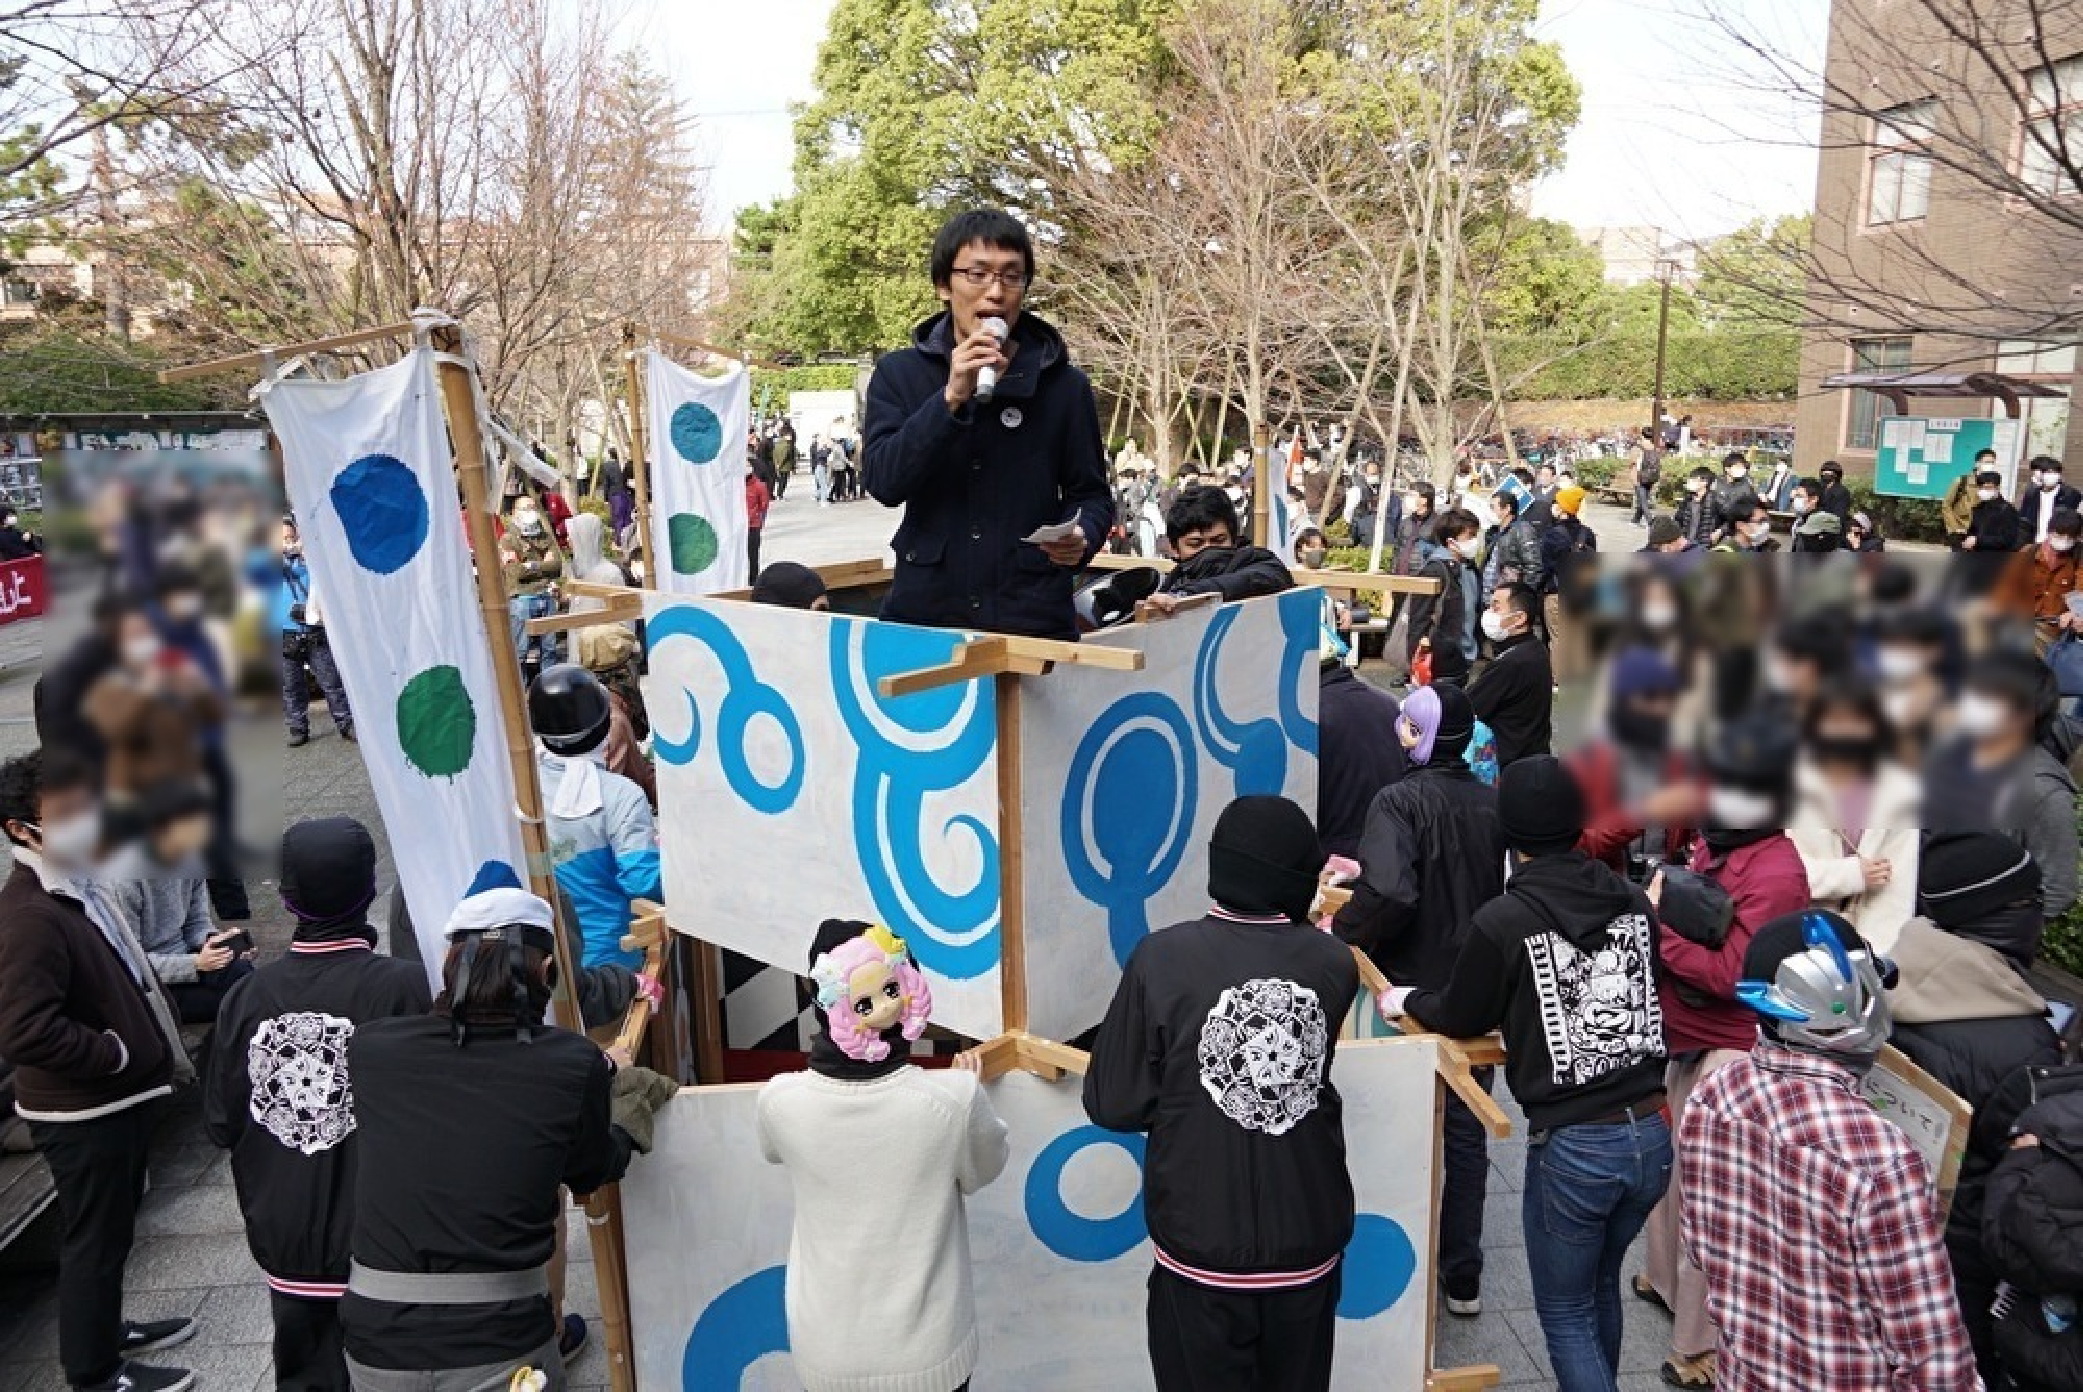
\includegraphics[width=18zw]{gazo/202112shukai.pdf}
    \captionsetup{labelformat=empty,labelsep=none}
    \caption{神輿に乗って演説する被処分者}
\end{wrapfigure}

 時計台占拠処分に向けた呼び出しが来た頃から全処対が主催して京大構内で集会が行われてきました。全処対主催で京大学生処分撤回・阻止 12 月緊急集会(通称「12 月集会」)が行われてきました。

 また、総長室突入を理由とした5学生への処分呼び出しが行われてからは熊野寮自治会主催での処分撤回・阻止集会も行ってきました。2024年7月に行った集会では、実際に呼び出しを受けている学生や大学当局によって言い渡されている学生含め熊野寮生が次々と発言に立ちました。当局は集会当日に大学職員を動員して集会への弾圧や出入り禁止の学生の排除を行ってきましたが、その場に集まった学生の力で出入り禁止処分を無効化して集会をやりきりました。文学部自治会学友会常任委員会や教員の先生方、他大学の学生団体からの賛同も得て広い陣形で集会を行うことができました。

 この集会には 2 つの意義があると思います。まず、多くの学生が集えば、当局がいくら集会を禁止しよう と集会できるのだと分かったことです。多くの学生が集えば表現の自由を守ることができるのです。逆に、表現の自由を守ろうという意志のもとにみんなが積極的に動かなければ、当局は簡単に学生の声を奪うことができたでしょう。権利や自由は当局によって与えられるものではなく、それを守ろうという不断の努力で私たち学生が作るものです。

 もう1つは、当局に対して、処分撤回・阻止で一致する学生の力を見せつけることができたことです。2019 年から多くの学生が不当な学生処分に対して声を上げ、集会や署名集めという形で行動を起こしてきたことで当局が下す処分の罪の重さ(停学期間の長さ等)が実際に軽くなっていたり、入試の像などの以前なら処分されていたことでも処分されなくなっていたりする現状があります。このように 多くの学生が集まれば集まるほど当局は処分を下しにくい状況、無期停学の解除や学生処分の撤回をせざるをえない状況に追い込まれるはずです。 


\subsection{お願い}
対処分戦略推進局はこれからも不当な処分攻撃に屈さず学生の権利を守っていけるよう活動を進めていきます。これを読んでいらっしゃる みなさんも、京大当局の動きに注意深く目を向けてください。当局が何か変なことをしたら、諦めるのではなく、立 ち上がってください。何をしたらいいのかわからなかったら、学部自治会や自治寮に顔を出してみてください。みな さんの力は学生の権利や自由を守ることに絶対に繋がります。w

\subsection{資料}


{\small
\begin{tcolorbox}[colback=white, colbacktitle=gray!30!white, coltitle=black, title=2024年9月25日付で京大生5名に下された懲戒処分に対する抗議声明,breakable]\index{せいめい@声明|(}

 2024年9月25日、2022年度熊野寮祭企画「総長室突入」に参加した熊野寮生5名に対し懲戒処分(うち1名に対し二ヶ月停学、4名に対し一ヶ月停学)が京都大学当局により下された。我々熊野寮自治会は、この懲戒処分を京都大学当局による学生の異議申し立て活動に対する不当な弾圧として糾弾する。以下に理由を述べる。

\noindent ○総長室突入の正当性\\
 2022年度寮祭企画「総長室突入」は学生との対話を拒み強権的に管理強化を進める京都大学当局に対する抗議の直接行動として、以下のような事項を要求した。
    
    \begin{enumerate}
        \item 保健診療所を廃止前と同水準で再開すること
        \item コロナ禍に乗じたサークル規制をやめること
        \item 11月祭に対する介入をやめること
        \item 学生自治寮への介入をやめること
        \item 京都大学立看板規程を撤廃すること
        \item 学生の活動に対する警察導入をやめること
        \item 学生懲戒規程を撤廃し、2016年から続く学生処分を撤回すること
        \item 学生の自由な活動を制限する一方的な授業改革(CAP制)をやめること
        \item 教職員に対する非正規職化や雇用雇止めをやめ、無期雇用転換を積極的に行うこと
        \item 各学生自治組織、並びに教職員組合からの団体交渉要求に誠実に応じ、合意に基づいた大学運営を行うこと
    \end{enumerate}
    
 以上10項目は学生や教職員の一般的利益として極めて正当な要求であり、事実企画当日には200名以上の学生が参加した。しかし、京都大学当局は事前に学生との対話抜きに一方的に告示を掲示して本企画を禁止し、学生窓口である厚生課へ行けと学生に指示してきたのみならず、最終的には警察を学生との合意なく入構させ学生を排除しようとした。

 しかし、熊野寮自治会含め学生はこれまでも継続的に厚生課窓口を通じ再三京都大学当局に対し改善を要求し続けており、それでも当局による管理強化は止まらなかったがために本企画のような抗議行動が起こされているのであって、この抗議活動に対してもこのような対応をとった京都大学当局は自身に対する批判に対し極めて不誠実に対応していると言わざるを得ない。

 そして、本懲戒処分は「学生を扇動」し「喧騒を激化」したことを理由に寮生5名を停学処分にしているが、これは当局が自身への批判を取り合わずただ「喧騒」として矮小化して鎮圧しようしていることの現れであり、今回の懲戒処分が当局が管理支配を強権的に進めていく上での政治的な弾圧として行われていることを示している。「総長室突入」が熊野寮自治会によって主催され多くの学生も参加した大規模な抗議行動であったにもかかわらず今回の五人のみに対し懲戒処分が科されているのは見せしめであり、学生の抗議行動を萎縮させるものである。

 「総長室突入」によって明るみに出たのは、抗議者に対し一方的に警察を導入したり懲戒処分したりする、学生と対話などする気のない現在の京都大学執行部の独裁的な態度だったのである。

\noindent ○停学処分の重さ・プロセス的な問題点\\
 また、今回かけられた停学処分は処分対象者の学生に多大な負担を強いる過酷なものであり、その決定に至るまでのプロセスにおいても問題がある。

 停学処分は対象となる学生の大学施設への出入りの一切を禁止するにも拘らず学費を徴収するため、事実上の罰金刑としての側面が存在する。また、今回下された懲戒処分は休学中の学生の休学状態を強制的に解除し、学費の支払い義務を発生させている。これは学生に決して安くはない学費を罰金として科すことにより京都大学当局に抗議する政治的な発言を封じようとするものであって、強く非難されるべきである。

 特に今回の懲戒処分は9月の末に通達されたため9月の末のわずかな日数に対しても一ヶ月分の学費支払い義務がきっかり発生しており、一ヶ月停学の場合は二ヶ月分の、二ヶ月停学の場合は三ヶ月分の学費の支払い義務が発生している。これによって京都大学当局は定められた停学期間で実際に構内に入ることのできない期間と学費の支払い義務を最大化しようとしており、全く姑息な工夫であると言わざるを得ない。

 また、過去の懲戒処分と同様に処分の決定に至るプロセスには問題が存在する。懲戒処分の対象となる学生は、聞き取り・弁明の機会の付与と称して京都大学当局から呼び出しを受けるが、この呼び出しは非公開・証拠の提示なし・弁護士含む第三者の同伴禁止などの不当な条件の下で行われる。これでは強権的かつ恣意的な証言の解釈が行われる、本人の意思に拘らず謝罪と反省を迫られるといった危険性がある。そしてなにより当局に対して弱い立場にある学生に対し、権力を持つ当局が一方的に処罰を押し付ける不均衡な構図自体非常に抑圧的で不当なものである。

 さらに、今回の懲戒処分に至るプロセスでは教授会による自治もまた無視されている。文学部から送付された陳述の機会を与えるとする文書において、処分者のうち一名に対しては当初譴責処分が検討されていると記載されていたが、実際にその学生に降ったのは一ヶ月の停学処分だった。ここから、文学部教授会が譴責処分で懲戒処分を上申したにも関わらず、総長により決定が覆され、教授会の判断よりも重い一ヶ月の停学処分が下されることになったと推測される。比較的軽いものになったとはいえ譴責処分を上申した文学部教授会の判断自体もまた批判されるべきものではあるが、学内自治の重要な構成員である教授会の議論の結果を無視して、さらに重い懲戒処分を独断的に下した京都大学当局の行動は教授会自治も踏み躙る極度の横暴であり、現在の当局の管理強化を一方的に進める姿勢をよく示す悪質なものである。

\noindent ○学生処分の本質的な不当性\\
 そもそも今回の懲戒処分に限らず、近年京都大学当局が行ってきた学生の行動に対する恣意的な処分は全て不当なものであり、学生全体への抑圧に他ならない。

 2016年以降、京都大学当局は熊野寮生を中心とした10名以上の学生に対し懲戒処分を行ってきたが、過去のこれらの処分も今回と同様の性質を持っている。過去にも京都大学当局は「業務妨害」を口実に、大学当局による管理強化・自治寮への攻撃に抗議した学生に対して、学生の言い分は一切顧みずに学生懲戒規程を恣意的に運用することによって懲戒処分を濫用してきた。その結果、学生は立て看板の一方的な規制や窓口における職員の不正な行為など、大学に疑義があっても、処分のおそれを前に萎縮させられ、理不尽を強いられ、大学の規制を受け入れざるを得ない状況に追い込まれてきた。こうして自治破壊が行われてきたのである。

 学生処分の問題は処分の対象となった学生だけには限定されない全学生にとっての問題である。特に、当局による廃寮化攻撃を含めた管理強化に抗議した学生が恣意的に処分されている以上、学生処分の問題は廃寮の問題と一体であり熊野寮自治会として看過できるものではない。また、学生処分は、数十年来、国策としての大学改革が学生の声を無視して一方的に進められ、全国の大学が「採算を取る」ことを要求される中で、多くの学生寮が廃寮に追い込まれ、学生の学びは管理され、生活が破壊されてきたことと一体の問題である。現在東京大学をはじめ、全国の大学で学費の値上げが問題となっている。これは大学改革政策における学生の生活破壊の最たるものであり、許されるものではない。京大当局も熊野寮や吉田寮との交渉を一方的に打ち切って廃寮化攻撃を行い、保健診療所も反対の声がある中で廃止を強行し、学内のガバナンス強化を要する国際研究卓越大学制度に率先して応募するなど大学改革を先頭で推し進める張本人として存在している。以上のような「改革」の障害となる学生に対して処分が行われてきたのである。

\noindent ○終わりに\\
 以上のように、本懲戒処分は管理強化を独断で進めようとする京都大学当局が抗議する学生に対し下した恣意的かつ過酷な攻撃に他ならないのであって、最も強い非難の言葉に値するものである。京都大学当局に対し我々熊野寮自治会は、当該5学生に対する懲戒処分を即時撤回し、「総長室突入」の要求10項目を受け入れることを求める。

熊野寮自治会

\vspace{5mm}
\noindent ▼今回の処分で用いられた規程\\
「京都大学学生懲戒規程」(平成29年2月28日 達示第103号全部改正)
(\url{http://www.kyoto-u.ac.jp/ja/about/organization/other/revision/documents/h28/t103-28.pdf})


\end{tcolorbox}
}

{\small
\begin{tcolorbox}[colback=white, colbacktitle=gray!30!white, coltitle=black, title=熊野寮生3名に対する無期停学処分の撤回を求める声明,breakable]\index{せいめい@声明|(}

    \begin{flushright}
    京都大学熊野寮自治会
    \end{flushright}
    \begin{flushleft}
    京都大学総長 山極壽一 殿 
    \end{flushleft}
    
    2019年9月10日付けで熊野寮生3名に対し無期停学処分が下されました。3名の行った行為はどれも「職員の行為を妨害」したものであり、京都大学通則第32条第1項に規定する「学生の本分を守らない」行為であるとされたためです。今回の処分について、以下の2点から抗議します。
    
    \begin{enumerate}
        \item 大学職員の行為の正当性を検証する場がない\\
         3名の行為・言動は、京都大学当局(以下、当局)の一方的な決定とそれを遂行する職員に対する抗議として行われました。
    
         学生との話し合いが一切行われない中で、当局の決定に従う職員は自らの職務を強硬的・暴力的に全うしようとし、学生がそれに抗議すれば否応なしに処分が下されます。
        正当性が検証されていない職務行為への妨害を理由とした処分は撤回されるべきです。
        
        \item そもそも懲戒規程の内容が恣意的に運用できるものである\\
         「京都大学学生懲戒規程」(平成29年2月28日 達示第103号全部改正)において懲戒の対象は「学生の本分を守らない者」とされ、さらにここでは「京都大学の諸規程又は命令に違反した者」がその具体的な項目の一つとして記されています。
    
         これによって当局の意思決定及びそれに従う職員の行為に反する学生を恣意的に処分することができるため、この規程による処分は撤回されるべきです。
    \end{enumerate}
    
     今回の処分は、立て看板規制や吉田寮現棟明け渡し訴訟、11月祭への介入など、当局が学生への規制・弾圧を推進する渦中で行われています。
    
     今後も当局が抗議する学生を処分することは容易に想像でき、その影響は現在だけでなく未来の京大生にまで及びます。大学の在り方を考える学生の権利・主体性が剥奪され、当局の意思決定に学生が反論し抗議することすらできない状況は、理性と言論の府たる大学において看過されるものではありません。
    
     熊野寮自治会は、寮生3名に対する無期停学処分の即時撤回、今後同様の形で学生を処分しないこと、そして今後の大学運営においては当事者である学生との話し合いを踏まえたうえで意思決定がなされることを求めます。
    
    \begin{flushright}
    2019年10月18日
    \end{flushright}
    
    \vspace{5mm}
    \noindent ▼京都大学による公式発表「学生の懲戒処分について」(2019年9月12日)\\
    (\url{http://www.kyoto-u.ac.jp/ja/about/events_news/office/kyoiku-suishin-gakusei-shien/kosei/news/2019/190912_1.html})
    
    \begin{quotation}
    本学は、文学部4回生1名、工学部4回生1名、総合人間学部4回生1名を、令和元年9月10日付けで、以下のとおり懲戒処分とすることを決定しました。
    \begin{enumerate}
        \item 文学部4回生1名を、京都大学通則第32条に定める「学生の本分を守らない者」として、令和元年9月10日付けで同通則第33条に定める停学(無期)処分とした。
        \item 工学部4回生1名を、京都大学通則第32条に定める「学生の本分を守らない者」として、令和元年9月10日付けで同通則第33条に定める停学(無期)処分とした。
        \item 総合人間学部4回生1名を、京都大学通則第32条に定める「学生の本分を守らない者」として、令和元年9月10日付けで同通則第33条に定める停学(無期)処分とした。
    \end{enumerate}
    
    \vspace{4mm}
    \noindent 処分理由
    \begin{enumerate}
        \item 文学部学生
        
         当該学生は、平成30年8月9日、オープンキャンパス初日に本部構内のクスノキ東側に設置された巨大工作物の一部に座り込み、当該工作物を撤去しようとする職員の行為を妨害するなどした。
    
         また、当該学生は、平成30年9月27日及び同年10月18日、教育推進・学生支援部棟2階の厚生課窓口及び廊下において、不審者を取り押さえようとする職員の行為を妨害するなどした。
    
         これらのことは、京都大学学生懲戒規程第3条第5号「前各号に準ずる不適切な行為を行った」に該当し、京都大学通則第32条第1項に規定する「学生の本分を守らない」行為である。
    
         よって、本学は、今回の行為の事実関係について調査を行い、慎重に審議した結果、当該学生を停学(無期)処分とすることとした。
        
        \item 工学部学生
        
         当該学生は、平成30年9月27日及び同年10月18日、教育推進・学生支援部棟2階の厚生課窓口及び廊下において、不審者を取り押さえようとする職員の行為を妨害するなどした。
    
         また、当該学生は、平成30年10月3日、吉田南構内において立入禁止対象者を構外へ連れ出そうとする職員の行為を妨害するなどした。
    
         これらのことは、京都大学学生懲戒規程第3条第5号「前各号に準ずる不適切な行為を行った」に該当し、京都大学通則第32条第1項に規定する「学生の本分を守らない」行為である。
    
         よって、本学は、今回の行為の事実関係について調査を行い、慎重に審議した結果、当該学生を停学(無期)処分とすることとした。
        
        \item 総合人間学部学生
    
         当該学生は、平成30年9月27日及び同年10月18日、教育推進・学生支援部棟2階の厚生課窓口及び廊下において、不審者を取り押さえようとする職員の行為を妨害するなどした。
    
         このことは、京都大学学生懲戒規程第3条第5号「前各号に準ずる不適切な行為を行った」に該当し、京都大学通則第32条第1項に規定する「学生の本分を守らない」行為である。
    
         よって、本学は、今回の行為の事実関係について調査を行い、慎重に審議した結果、当該学生を停学(無期)処分とすることとした。
        
    
    \end{enumerate}
    \end{quotation}
    
    \vspace{5mm}
    \noindent ▼今回の処分で用いられた規程\\
    「京都大学学生懲戒規程」(平成29年2月28日 達示第103号全部改正)
    \url{http://www.kyoto-u.ac.jp/ja/about/organization/other/revision/documents/h28/t103-28.pdf}
    
    \vspace{5mm}
    \noindent ▼補足\UTF{2160}.不審者取り押さえ時の状況
    
     3名に共通する処分理由である上記の「平成30年9月27日及び同年10月18日」の件は、熊野寮自治会による要求書提出の際に起こった出来事です。この際、2017年7月25日付で京都大学を放学処分となり、同年10月2日付で学外者として敷地内立入禁止とされた\UTF{9AD9}田暁典がストッキングとフルフェイスヘルメットを被り、水色のネズミの着ぐるみを装って提出行動に参加していました。10月18日の要求書提出後、職員約8名が彼を取り押さえ、顔を隠した素性不明の不審者として警察に引き渡し、不退去罪の現行犯として逮捕させました。\index{ようきゅうしょ@要求書}
    
     職員は退去しようとしていた\UTF{9AD9}田を大人数で取り押さえ、その手を踏みつけて流血させ、彼の退去を暴力的に阻止していました。この取り押さえ方に対し、寮生3名は職員と高田の間に割って入る、職員を高田から引き剥がすなどして、それを阻止しようとしました。
    
    \vspace{5mm}
    \noindent ▼補足\UTF{2161}.近年の京大内の管理強化について
    
     ここ数年、大学職員は顔を隠して活動する学生を取り締まっています。顔を隠した状態で学内に入ろうとする学生に対し素顔をさらせと職員が要求し、拒否した学生に対しては不審者と断定し学外に強制的に排除します。顔を確認することで個人を特定し、学内での行動を逐一監視したり、学部・研究室\index{けんきゅうしつ@研究室}の教授を通しての脅しをかけたりなど、あらゆる形で学生に対し圧力をかけています。オープンキャンパスなどで着ぐるみを着て学内で宣伝活動している学生もいますが、顔を隠している学生は無条件で全員排除というわけではなく、職員の一存で強制排除されるかどうかが決まります。
\end{tcolorbox}
}

  \newpage
  \section{ガサにまつわる大学と寮自治会の立場}
\label{sec:gasa_jiti}
	熊野寮には昔からよくガサ(家宅捜索)が入ります. このガサについて説明します.\index{がさ@ガサ}

		\subsection{捜索の原因}
		\emphbf{捜索の原因は中核派だとされているが, その捜索自体が不当であり, 熊野寮が中核派を追い出すことはない. }\footnote{熊野寮自治会「Campus Life News Vol.12 について」(2017年5月16日)参照}\index{ちゅうかくは@中核派}

 		川添信介副学長は2017年2月14日発行の「Campus Life News Vol.12」において, 「熊野寮の捜索」という文章を発表しました. この文章では, 捜索が行われる原因は中核派が住んでいることであり, 追い出すべきであると述べているように見えます. しかし, 熊野寮自治会が中核派を追い出すことはありませんし, いかなる思想や信条を理由に入寮を拒むことは決してありません.

		なぜなら, 家宅捜索が行われる目的が事件の捜査だとは思えないからです. 当時の捜索は「ある中核派の学生が裁判所で退廷命令を下され, 両脇を抱えられながら法廷警備員の右膝を蹴った」という公務執行妨害事件についての捜索でしたが, 事件から10ヶ月以上も経ったあとにその学生が逮捕され, 熊野寮への捜索が行われました.

		「蹴った」という行為の証拠が10か月後の熊野寮から出てくるとは到底思えません. また, 家宅捜索では大量の機動隊員が動員されました. 過去に寮生が捜索を妨害したことはありませんし, 必要のない捜索を, 必要のない機動隊の動員\index{きどうたい@機動隊}とともに行っている理由は, 寮生や近隣住民を怖がらせたり威圧したりするためだというのが寮自治会の見解です.

 		大学の教員にも, 真理を探究する一研究者として, 法的正当性とは必ずしも合致しない「正しさ」について自ら考え行動してほしいものです.

		\subsection{寮生とともに大学当局も抗議する}
		先述の「確約書」項目Eにおいて大学職員も「その場で抗議する」ことになっています. 責任者間だけではなく, 各職員が各捜査員に対して, 現場で即座に抗議する, ということが当局と自治会の間で確認されています.

		過去には, 2009年5月18日付で, 大学職員が立会を行なうために十分な機会と時間を与えずに警察官が熊野寮の敷地及び建物に入ったこと, 玄関を必要もないのに過剰な人数の機動隊員で占拠し, 寮関係者の出入りを規制したことに抗議する文章を当時の副学長が警視庁警視総監と京都府警・大阪府警に申し入れています.

 		しかし, 「玄関の過剰警備に抗議して下さい」という現場での寮生の要請に対して「後日責任者間で行うから, 今はしない」というような返答をする事務職員も確認されており, これは確約違反となります.

 		もちろん, 過剰警備だけでなく無関係な物件の押収・撮影など多くの不当行為に対し, 学生の生活を守る立場として真摯に抗議する職員・教員も少なくないです. しかし, 個人単位で確約の内容を無視する者がいることも事実であり, そういった事実が確認される度, 当局がその点を改善するよう, 自治会から要求をしています.

       
  \section{ガサについて抗議すべき点}
\label{gasa_kogi}
	ガサの不当な点は大きく二つ, 「捜索自体の不当性」と「現場での不当行為」に分けられます. 以下の観点に基づいて寮生は抗議しています.

		\subsection{捜索自体の不当性について}
		 わかりやすい例を挙げると, 2013年にあった事案で, 「令状の捜索目的が熊野寮と無関係である」というようなことです. 寮生ではないし, 過去に住んでいたこともなければ, 立ち入ったこともない人物の被疑事件で令状が出されており, 自治会から抗議の声明を出していました.\index{せいめい@声明}


    
    

		\subsection{現場での不当行為について}

			

			\subsubsection{過剰警備}

			\begin{wrapfigure}[18]{r}[1cm]{8cm}
				\centering
				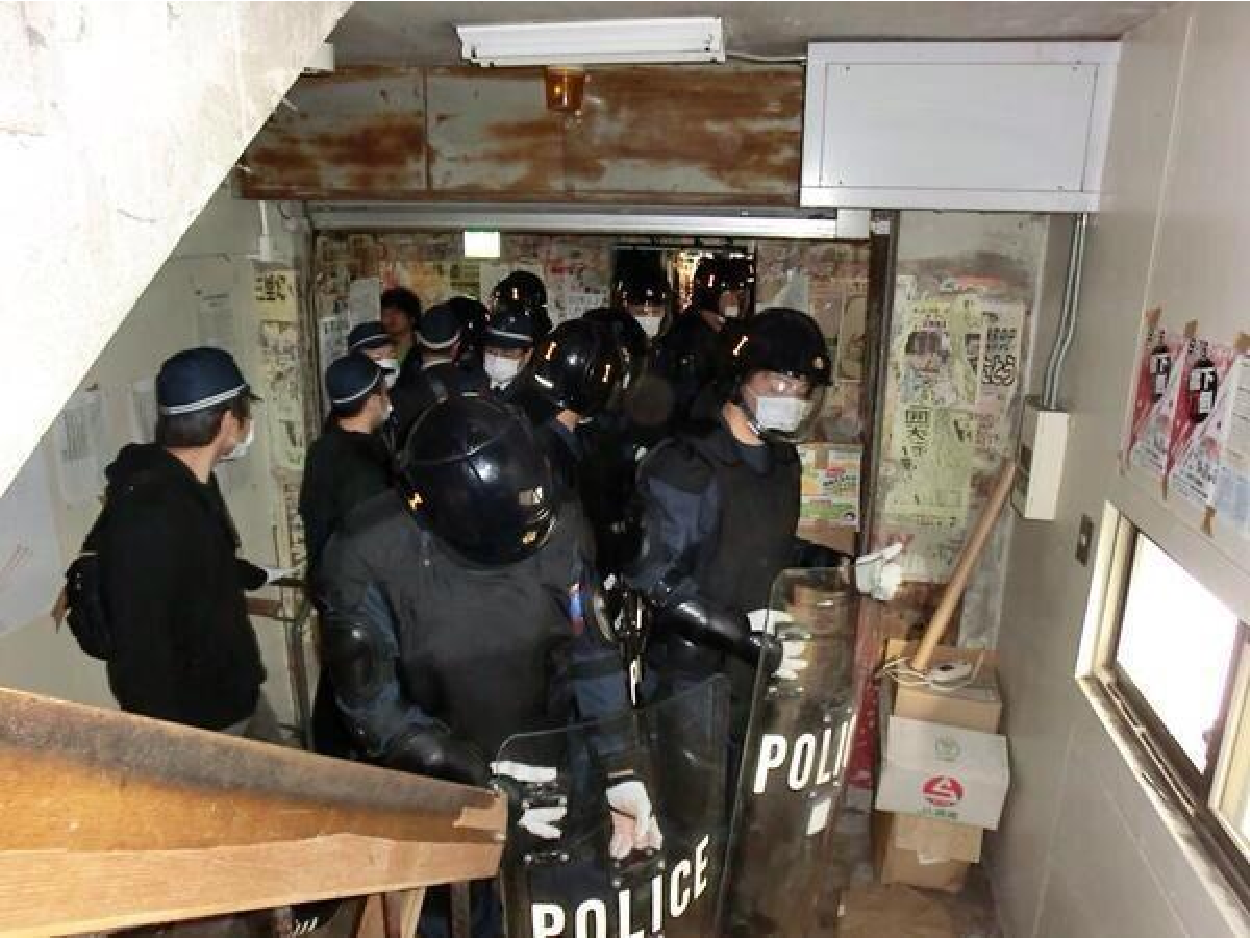
\includegraphics[width=7.8cm]{gazo/gasa.pdf}
				\caption*{\small{B棟1階階段周辺を占拠する機動隊}}
			\end{wrapfigure}

			捜索場所が1部屋のみで, 捜査員10名で足るような状況であっても, 50〜150名の機動隊を動員し, 玄関および捜索場所に至るまでの階段と廊下を不必要に占拠されるのが毎度のことです. 明らかに過剰な警備であり, 寮生の生活を不当に破壊するものとして抗議しています.
			
      
			\subsubsection{令状の不提示}
			令状を示すことなく押し入ることがあります. 本来は敷地に入る前に提示すべきものです. 2017年1月のガサで久しぶりに正門前での提示がありましたが, 2013年からそれまで正門前で提示されたことはありませんでした.

			\subsubsection{警察手帳不提示}
			「提示の必要はない」とはっきり言い放つ捜査員が度々現れますが, 人の住居を占拠しておきながら, 自身が警察官であることを示さなくてもよい, というのは一体どういうことなのでしょうか.

			「警察手帳規則第5条(証票及び記章の呈示) : 職務の執行に当たり, 警察官, 皇宮護衛官又は交通巡視員であることを示す必要があるときは, 証票及び記章を呈示しなければならない」に違反していると考えられます.

			\subsubsection{無関係な寮生の撮影}
			捜査員が, 廊下などの過剰警備に抗議する寮生や授業に出ていく寮生を終始撮影することがあります.

			警察官は捜査に際し, 捜査に関係の無いものを押収・撮影してはいけないとされています. よって, 公安警察の行為は肖像権の侵害にあたり, また, 憲法十三条をみても違憲行為であると考えられます. このような事例に関し, 捜査に無関係な第三者の撮影を違憲・違法とする最高裁の判例もあり, 言い逃れは不可能です.

			\subsubsection{2021年、2023年のガサでは機動隊は入構しなかった}\index{きどうたい@機動隊}
			2021年6月、2023年4月のガサでは正門前で寮生が警察に抗議した結果、機動隊は正門前で待機し、私服の捜査員のみが入構し捜索を行いました。\emphbf{機動隊が寮内で警備に当たらなくても、粛々と安全に捜索できることが証明される形になりました。}
			

\chapter{寮生の声}
  

\section{深夜徘徊のすすめ}
文責:雁音
\subsection{はじめに}
入寮パンフを手に取ってくださったみなさま、特にこの記事に目をとめてくれたみなさま、お読みいただきありがとうございます。今年はどんな記事が寄稿されているのでしょうか。入寮パンフに文章を載せていただくのは今回が初めてなので、すこし肩肘を張っているかもしれませんが、どうか最後までお目通しいただければ幸いです。\\ \indent 
さて、熊野寮には数多くの趣味コミュニティが存在しますが、そのひとつに深夜徘徊部があります。深夜徘徊というと、夢遊病かのような印象のある語彙ですが、実態としては「深夜散歩」なんかが近いです。目的地がなかったり、ありえない距離を歩いていたり、結果帰寮が朝だったりするので、かえって散歩より徘徊の方がニュアンスが適切かもしれません。とかく、僕たちの趣味たる深夜徘徊について魅力を伝えられたらなと思い、発案に至りました。\\ \indent 
京都という街は深夜徘徊に本当に適しています。京都に惹かれて京大を受けた、そこの非関西勢!僕と同じですね。ぜったいにハマるので、入寮した暁には、ぜひとも一緒に行きましょう。

\subsection{本編}
あらためて、はじめまして。入寮3年目の雁音といいます。3年目って本当ですか…?全然実感がない、まだ2年目くらいの気分。かるく自己紹介をすると、緑茶とスマブラとピアノと哲学と化学が好きな人です。それぞれ話すと大変なことになってしまうので、入寮面接や入寮後にお話しする機会があればということで。深夜徘徊には入学して一か月後くらいには行き出していたのですが、ひとと行くようになったのは実は最近なんですよね。雑談の機会としては勿論、自分と違う視点で街の解釈を語ってくれるのもとっても愉快です。熊野寮は全体的に話し合いが実に盛んな場所です。それは運営方針の擦り合わせやトラブルの解決という分かりやすい手段に留まることなく、談話室の存在による日常的な対話の多さや、一緒に生活を営み、お互いの解像度が上がることによる立ち入る内容の深さが特徴的な文化となっています。それがゆえに、寮生は話の構成や言語化が上手だったり、自分の好きな分野への熱意や知識量が豊富だったりして(これは京大全体に言えるかもしれませんね)、とかく話していて楽しいです。\\ \indent
少し話が逸れました。以下では、深夜徘徊の何が好きなのか言語化すること、好きな写真から語ることに分けて発信していこうと思います。どのくらい長くなるか分かりませんが、しばしお付き合いいただければと思います。\\ \indent
\subsection{何が好き?}
深夜徘徊の魅力を「深夜」と「徘徊」の要素に分解してみます。まずは「深夜」から。分かりやすい点から行くと、人が少ない!これは本当に魅力的です。過剰なひとごみが苦手で、さらに言えば、それがゆえに景色の本来の姿が見えなくなることが悲しい僕としては、深夜の人の少なさにはかなり救われるものがあります。夜の景色は(昼の景色に対し、多くの場合で)本来的ではないと言われてしまうとその通りなのですが、体感としては、昼夜というワンセットは「自然の」摂理としてそこにあるので、夜の景色も見つめたいなあと思っています。これに関連して、根本的に深夜はものが見えにくいので、意識しないものを見ずにいられるというのも良いですね。深夜だとニュートラルに流れ込む情報量が少ないので、考え事をしたり、ひとと腰を据えて(歩いていますが、)話したりする上で良く作用します。もちろん、単に落ち着くというのもありますね。\\ \indent
「徘徊」については、散歩と魅力の多くが共通していると思います。より正確に言うと、目的のない散歩です。たくさん歩くのって楽しいですよね。運動不足がちな寮生においては健康にも寄与しています(昼であればより健康…)。熊野寮には「エクストリーム帰寮」という寮祭企画があります。目隠しをして車に乗り、寮から遠く(20km~100kmが標準的?)に飛ばされ、徒歩で帰寮するというコンセプトの企画です。これと同じように、意味不明な目的地を設定したりしなかったりして、長距離を歩くというのは僕を惹いて止みません。地球上どこでもそうですが、特に京都で顕著なこととして、長距離を歩くと街並みの変遷が実感できて面白いということがあります。京都の街並みが好きで進学した場合はなおのこと!ひとと歩く場合ならば、街を題材に話のネタが尽きないというのも地味に推しポイントです。\\ \indent

\subsection{好きな写真たち}
\begin{figure}[H]
    \centering
    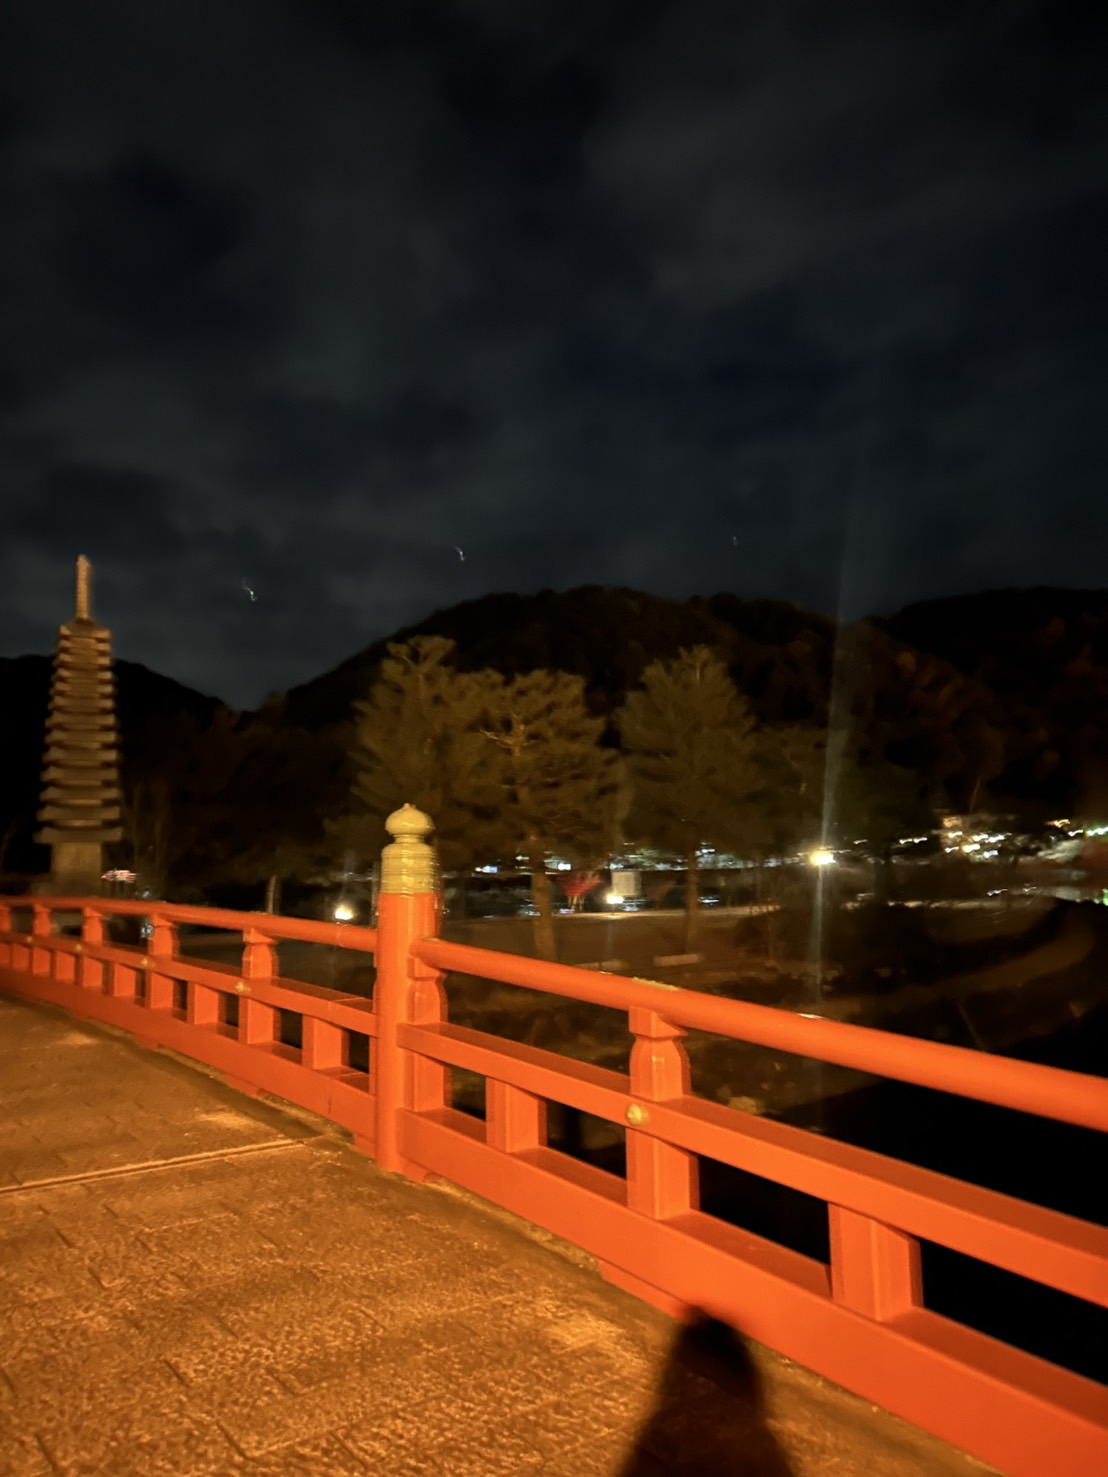
\includegraphics[width=5cm]{2025shinki/shinya_haikai/image1.png}
    \caption{@宇治公園}
    \label{fig:enter-label1}
\end{figure}

深夜と朱色ってめちゃくちゃ良いんですよね。京都には朱色が多くて、うれしい限りです。静寂の宇治公園の中では川の流水音も聞こえるのですが、これもたまらない。安易に歩いて行くには
遠すぎるという点を除けばきわめて好みのスポットです。印刷だと白黒になってる気がする、というか悪くすると真っ黒になっている…?祈るばかりです。

\begin{figure}[H]
    \centering
    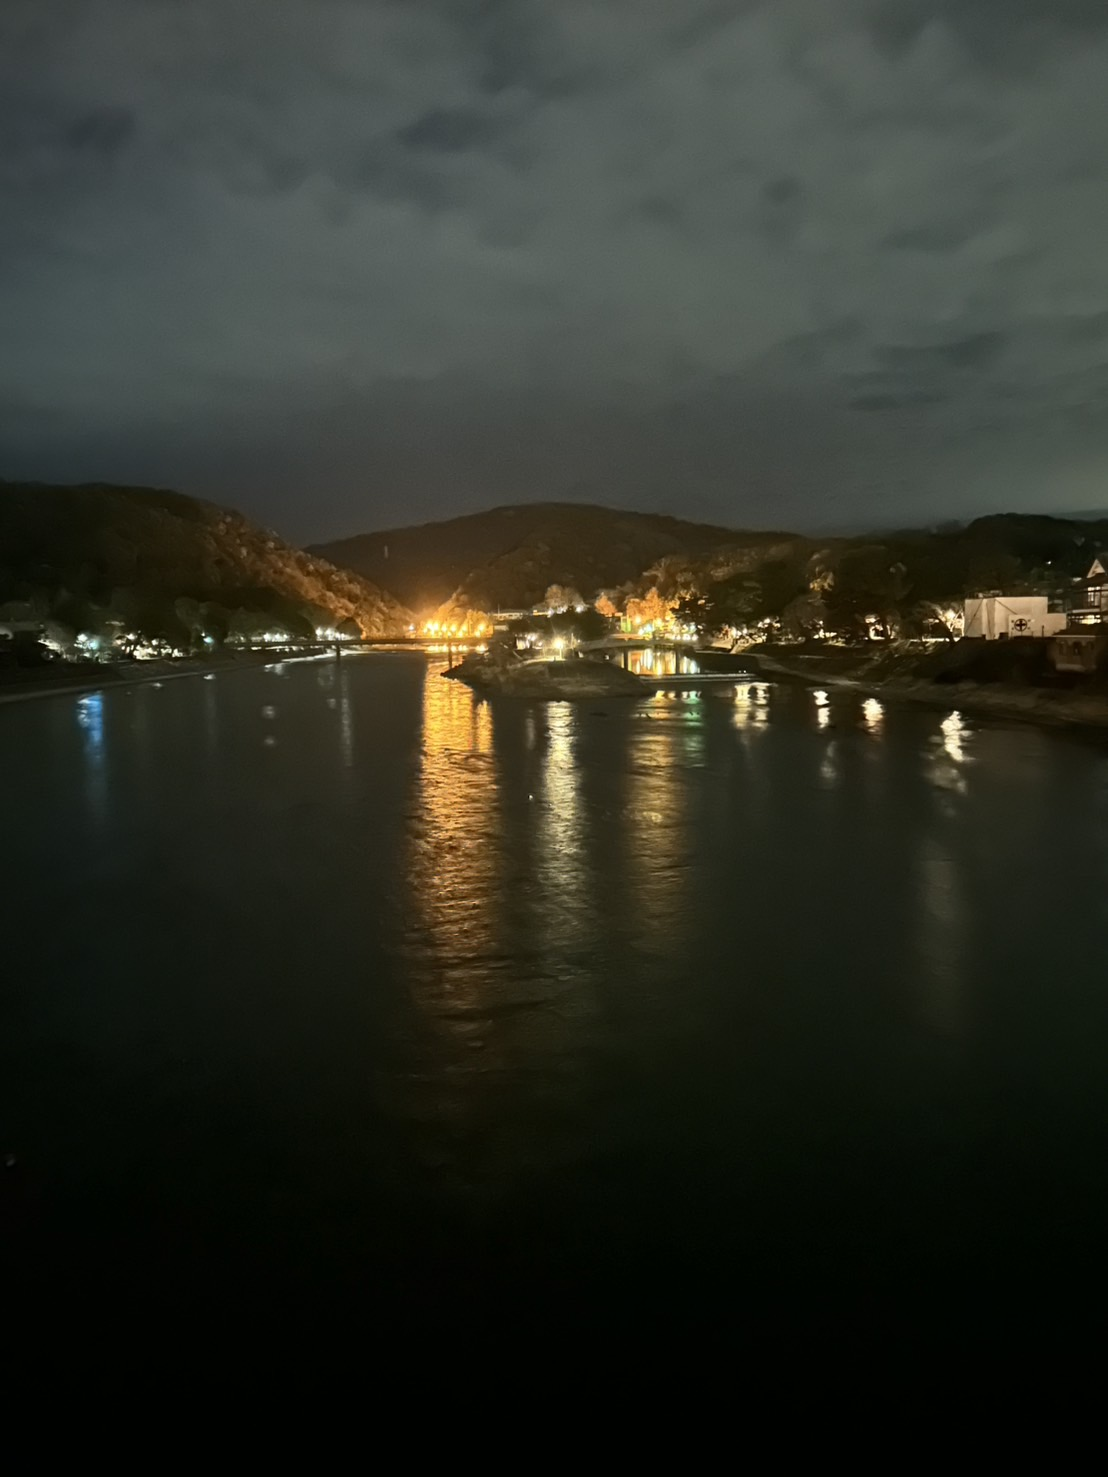
\includegraphics[width=5cm]{2025shinki/shinya_haikai/image2.png}
    \caption{@宇治川}
    \label{fig:enter-label2}
\end{figure}
深夜と川ってめちゃくちゃ良いんですよね。背景の山によるレイヤーも明かりも川への反射も良い。これで月とか写っていれば最強でした。川や湖面に映る光の揺れ加減にあらわれる各人のフェティッシュを聞くのが大好きです。

\begin{figure}[H]
    \centering
    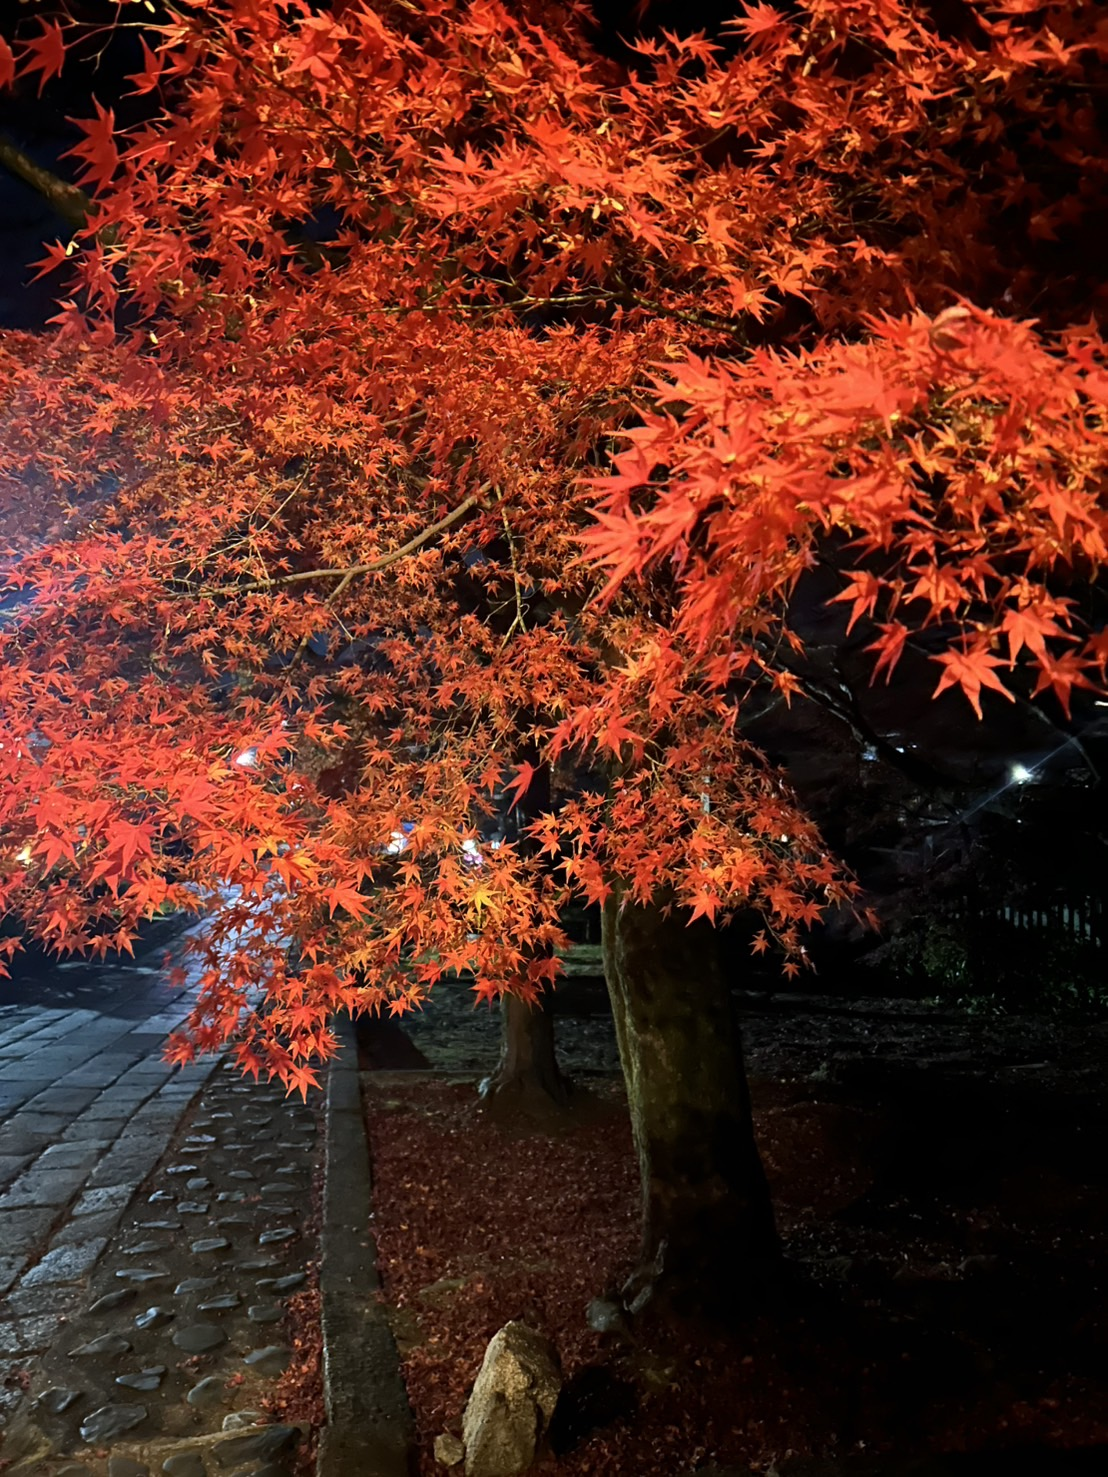
\includegraphics[width=5cm]{2025shinki/shinya_haikai/image3.png}
    \caption{もみじ}
    \label{fig:enter-label3}
\end{figure}
深夜ともみじってめちゃくちゃ良いんですよね。となりに映る道も夜であるが故の艶やかさが感じられて好みです。季節限定ですから、寒さを乗り越えてがんばって歩きましょう。新入寮生に向けて言えば夜桜もとってもおすすめなのですが、いま手元に写真がありませんでした…一緒に撮りに行きましょう!

\begin{figure}[H]
    \centering
    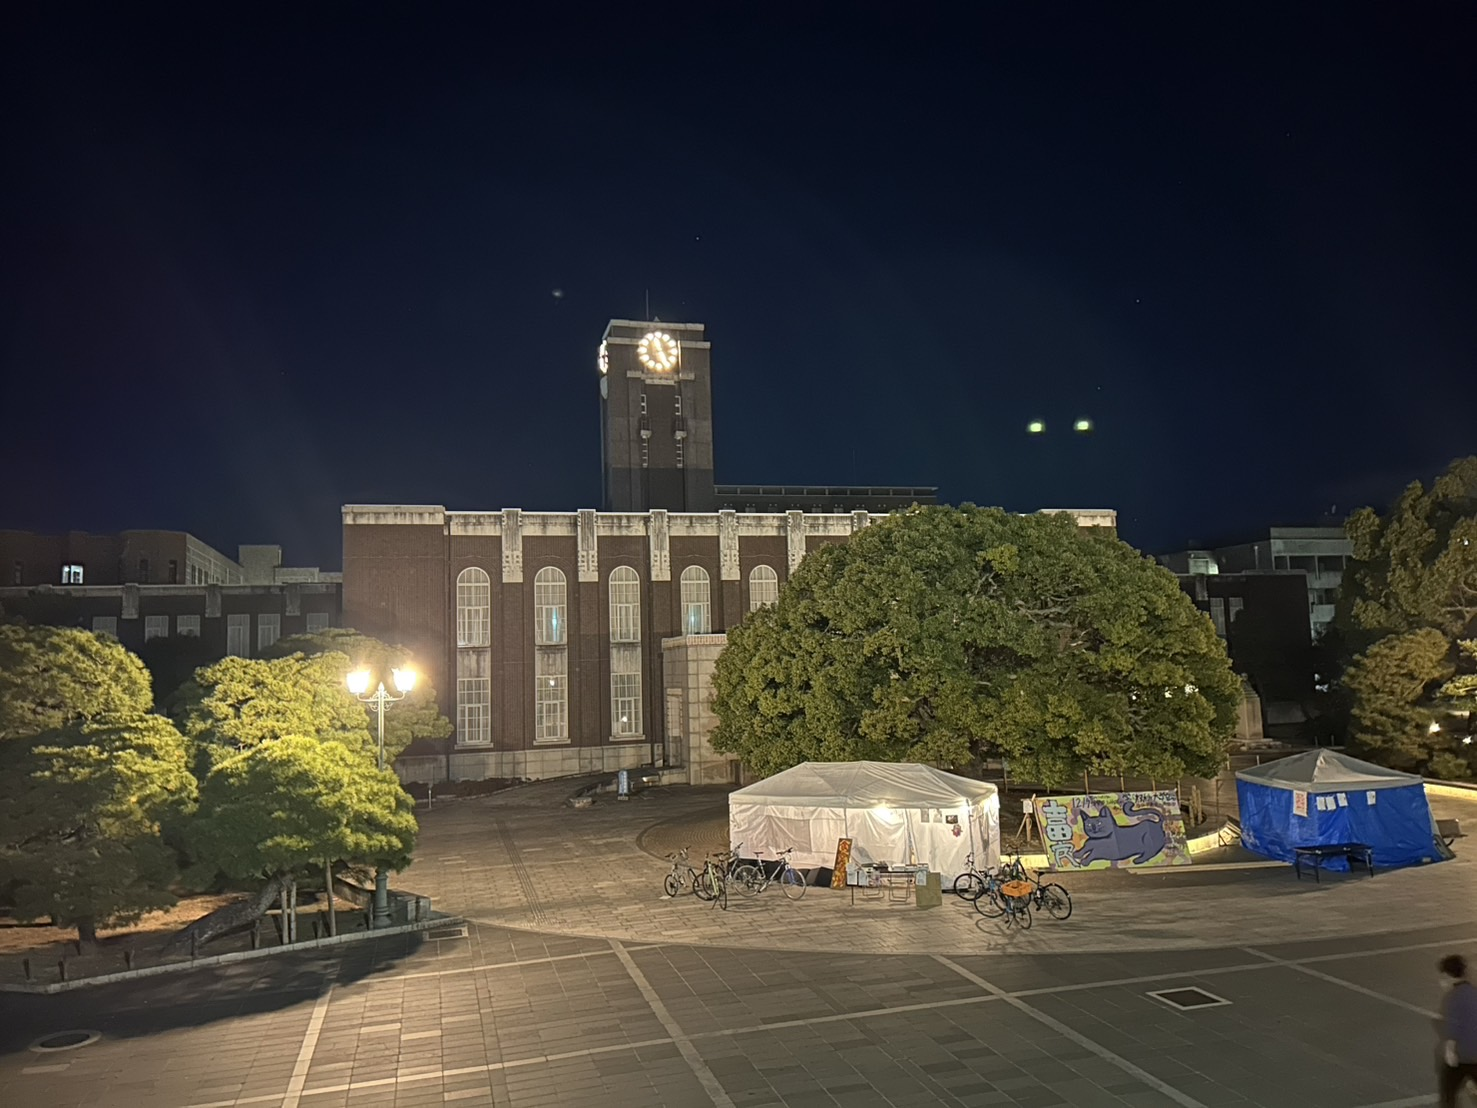
\includegraphics[width=5cm]{2025shinki/shinya_haikai/image4.png}
    \caption{@京都大学}
    \label{fig:enter-label4}
\end{figure}
京都大学に深夜に侵入すると、実はできることが多くて楽しいですよ!ここでは具体的には書きませんが、入寮後にたくさん語りたいと思います。写真中のテントは吉田寮のものですが、熊野寮でもキャンパス情宣といって、楠の前にテントを立てて夜を明かす活動を行っているので、ぜひ体験してみてください。\\ \indent

以下は部員から提供された写真になります。(紹介文もいただきました!)
\begin{figure}[H]
    \centering
    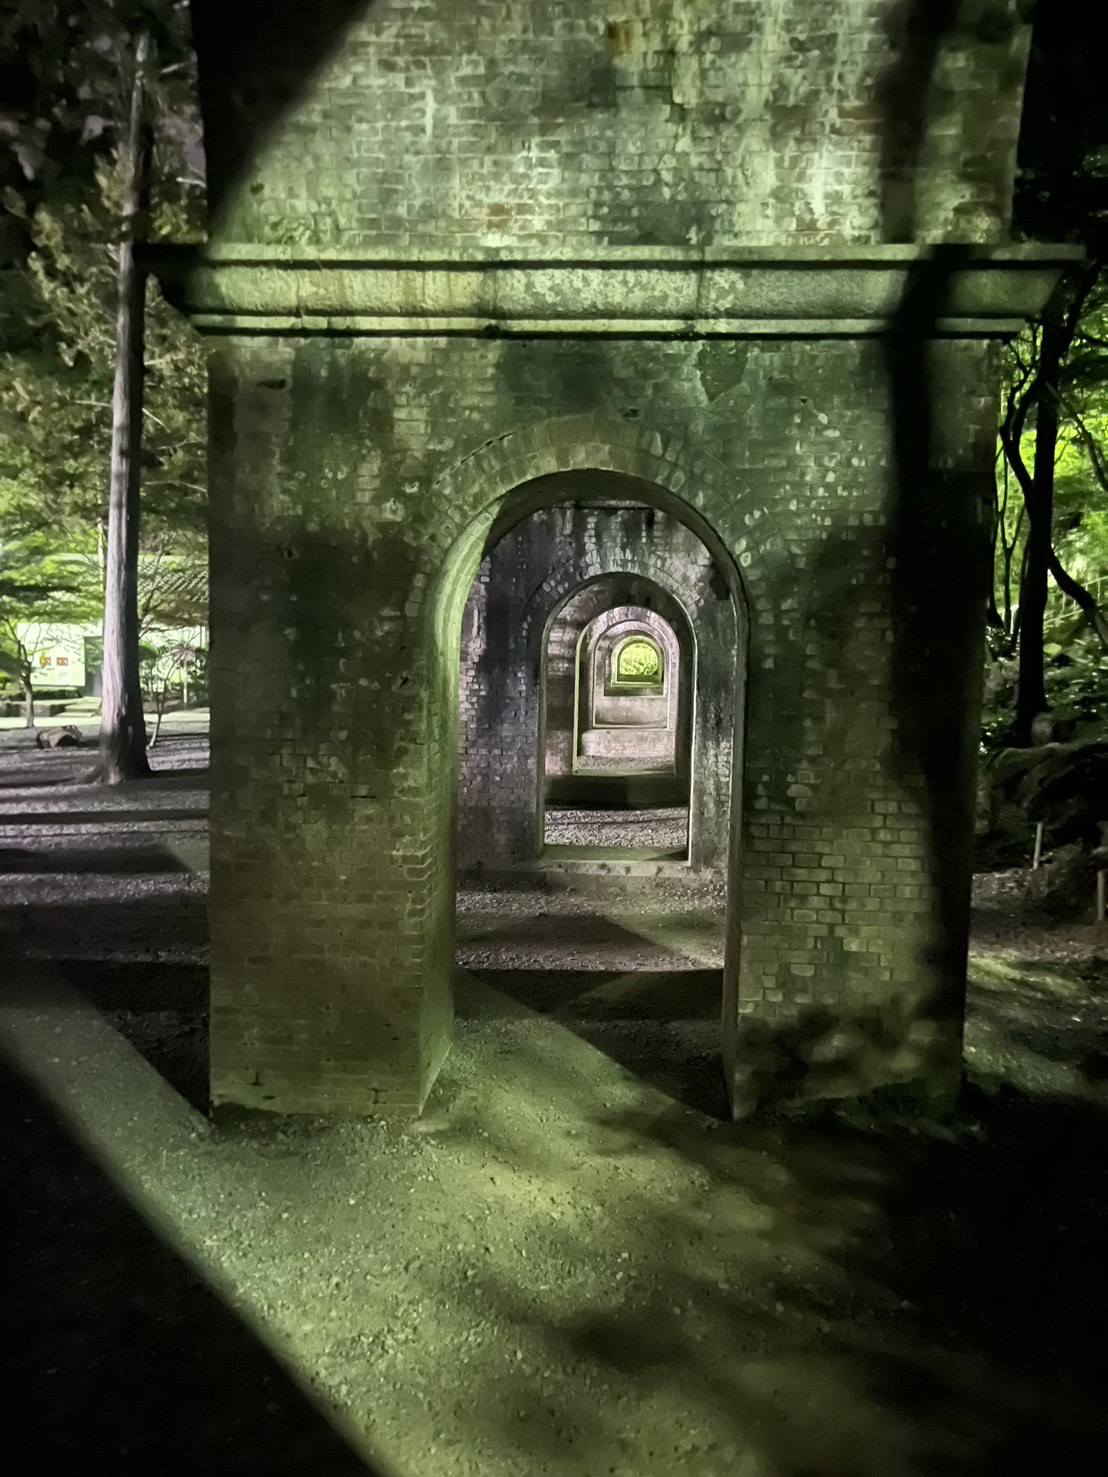
\includegraphics[width=5cm]{2025shinki/shinya_haikai/image5.png}
    \caption{南禅寺水路閣}
    \label{fig:enter-label5}
\end{figure}
人気のフォトスポットなので、知っている人もいるかもしれません。南禅寺は寮から適度に近く、深夜徘徊先として優秀です。敷地が広くて落ち着いているし、塔頭もたくさんあって、外の世界とは違うひとつの街を構成しているようでお気に入りのお寺です。昼間に行くのもいいですが、この写真のように人が一人もいない水路閣は夜しか見ることができません!周辺に植えられているもみじも綺麗で、個人的には南禅寺は紅葉より青もみじが好きです。


\begin{figure}[H]
    \centering
    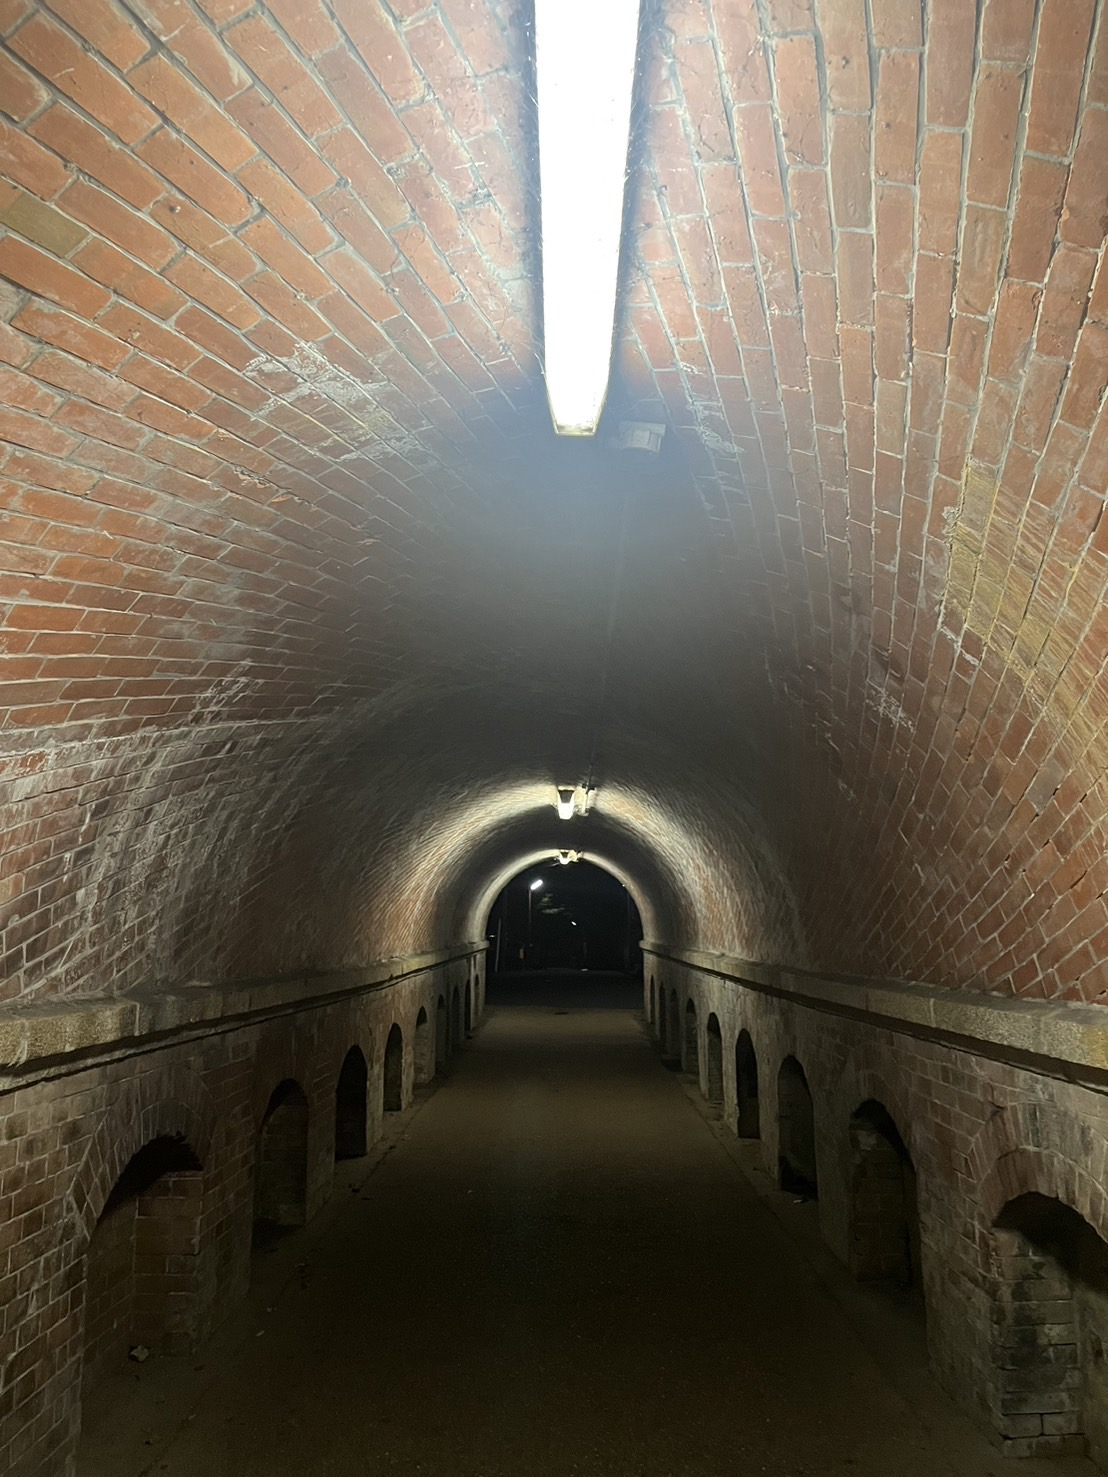
\includegraphics[width=5cm]{2025shinki/shinya_haikai/image6.png}
    \caption{琵琶湖疏水ねじりまんぽ}
    \label{fig:enter-label6}
\end{figure}
ここも南禅寺界隈です。「ねじりまんぽ」というのは「ねじりのあるトンネル」を意味しています。螺旋状に煉瓦を積み上げることで強度を確保しているそうです。トンネルってある世界とある世界を分ける役割を果たしていると思うんですが、このトンネルもそれに漏れず、落ち着いた、どこか異世界感のある南禅寺と多くの車が行き交う三条通とをくっきりと分けています。また、煉瓦が螺旋状に配置されていることで、より違う世界に行く感覚が強くなっている気がします。


\subsection{おわりに}
やっと書き終わりました(午前3時)。乱文で申し訳ありません。深夜徘徊部にもかかわらず普通に眠いです、いまから寝ます。著しく締め切りを過ぎての寄稿に謝罪するとともに、編集してくれる皆さんに感謝を申し上げて結びとしたいと思います。読んでくれた皆さん、また話しましょうね~~~~

  \newpage
  \subfile{2025shinki/nuigurumi_zadankai/nuigurumi}
  \newpage
  
  \section{ボドゲの定石を作る 〜WINGSPANを題材にして〜}
  
\setlength{\abovedisplayskip}{5pt}
\setlength{\belowdisplayskip}{5pt}

\rightline{(文責:アメリカムシクイ)}

\subsection{はじめに}
\begin{multicols}{2}
ボードゲームは、麻雀と並ぶ寮内娯楽の一つである。麻雀は年に2度全寮的な麻雀大会が開かれるほどには寮生の間に浸透しており、どの談話室でも遊ばれている。一方でボードゲームは麻雀ほどメジャーな遊びではないものの、ボドゲ新歓という食堂でボードゲームを遊ぶ交流会が開かれる程度には人気な娯楽だ。寮でよく遊ばれるボードゲームは、カタンやとドミニオンでろう\footnote{中でもカタンは私が一番好きなボドゲだ。寮祭で耐久カタンという企画が開かれるほどには人気で、\sout{正直ウィングスパンをしながら「こんなことやってないでカタンの研究がしたい」といつも思っている。}一方でウィングスパンはどちらかというとマイナーで、私が存在を確認している談話室は3か所しかない。そのうち1つは私がこの記事の原稿を書き終えた後に布教した。}。この2つは寮のどこの談話室に行っても大抵置いてある。そして、本記事で扱うWINGSPAN(ウィングスパンと読む。)も数多あるボードゲームの一つだ。
\par
先日(と言ってもこの入寮パンフレットができあがるころには1年近く経ってしまっているが)、知り合いの寮生たちの間で開いた耐久ボドゲ会\footnote{一日中ボドゲをして遊ぶという尊くて幸せな会。私がよく主催して、知り合いのボドゲ好きな寮生たちと遊んでいる。通常「耐久する」という言葉は、夜通し何か一つのことをして徹夜するという行為をさす。例えば耐久麻雀と言えば、徹夜で麻雀をするという意味である。ただ徹夜をするのは身体が耐えられないので、夜の代わりに昼間に遊んでいる。}で、ウィングスパンを遊ぶ機会があった。第2章で述べるようにウィングスパンは各プレイヤーが鳥の生態系を作るゲームであるが、私は以前から、こうした自分の世界で拡大再生産するタイプのボドゲがあまり得意ではなかった。たいていこの種のボドゲはAを作るのにBが必要で、Bを作るのにCが必要で、Cを作るのにAが必要、といった具合に、ゲームで必要になるものを作るための手段が巡り巡ってループしており、序盤に何をすべきかがいつも分からないからだ。その会でもコツが掴めないままゲームが終わってしまったが、ゲーム自体は参加者に好評であった。せっかくみんなが好きになってくれたならと、苦手克服のために研究を始めることにした。
\par
ウィングスパンの苦手なところは序盤に何をすべきか分からない、ということであったから、始めた当初は序盤の定石を明らかにしたら終わりにしようと思っていた。しかし、研究を進めるにつれて、初めに想像していたよりも定石の分岐が複雑だということが分かり、より深く調べるために鳥カードの分類を始めてしまった。しまいには談話室の雑記帳の半分近くが研究の進捗で埋まり、ウィングスパンにある170羽の鳥の分類表を完成させるに至っていた。廃人になるまで1か月もかからなかった。
\par
あまりにも成果が多かったことと、談話室の雑記帳にとどめておくだけではもったいないと思ったことから、今回入寮パンフの記事として書くことにした。寮内のプレイヤーが少ないボドゲの考察記事を書いたところで喜ぶ人がどれくらいいるかは分からないが、この記事が寮のボドゲ文化のさらなる盛り上がりに寄与したらとてもうれしい限りである。
\par
次章に入る前に、本記事の構成を述べる。最初にウィングスパンの概要としてルール、得点方法について述べる。その後これらの情報から理想的な立ち回りを一つ提示し、その立ち回りがうまくいかない場合を例外として整理する。最後に個々の例外に対して対処法を与え、理想的な立ち回りの一例を完成させる。なお、ウィングスパンには拡張版がいくつかあるが、本記事で考察するのは無印のものに限ること、加えて研究はオートマ戦(一人プレイ)をもとにしたことをここで言及しておく。
\end{multicols}
\subsection{WINGSPANの概要}
\begin{multicols}{2}
\subsubsection{ルールの概要}
考察に入る前に、ウィングスパンのルールについて概説する。ルールをご存じの方は飛ばしてもらって構わない。
\par
ウィングスパンは各プレイヤーに配られたゲームボードに鳥カードや卵を配置していって、プレイヤーごとに生態系を作っていくゲームである。4ラウンド合計26ターンをかけて生態系を作り、ボード上の様々な要素に対して与えられた得点の合計を計算して、最も多くの得点を得たプレイヤーが勝者となる。基本は2~5人で遊ぶものだが、1人で遊ぶためのルールもあり、私のような独り者にも優しいボードゲームとなっている。
\par
ゲームが始まる前に各プレイヤーは5枚の鳥カードと2枚のボーナスカードが配られる。鳥カードは鳥の絵柄が書かれたカード、ボーナスカードは鳥カードに関する条件が書かれたカードで、その条件の達成度合いに応じてゲーム終了時に点数が得られる。プレイヤーはそのうち鳥カードを好きな枚数捨て、捨てた数と同じ種類だけ餌トークンを1個ずつ得る。そして2枚のボーナスカードのうち1枚を選び、選ばなかった方を捨てなければならない。ここまでが最初の準備である。
\par
各プレイヤーが最初の準備を終えた後は、プレイする順番を決め、1ラウンドの1ターン目からゲームが始まる。そのターンですべてのプレイヤーがプレイしたら、今度は1ラウンドの2ターン目になり、また1ターン目と同じ順番でプレイしていく。ラウンドが変わるごとに最初にプレイする人を変えながら、26回これを繰り返す\footnote{1ラウンド目は8ターン、2ラウンド目は7ターン、というようにラウンドが1つ進むごとにそのラウンドでのターン数は1つずつ減少していく。}。また、ラウンドごとにラウンド終了時目的というものがランダムに決められており、その達成度合いによりプレイヤーごとに点数が配分される。そのため、各プレイヤーはラウンドごとのラウンド終了時目的を達成できるように、さらにゲーム全体を通してボーナスカードの条件をできる限り達成できるように、プレイすることとなる。
\par
各ターンでプレイヤーができることは鳥カードのプレイ、餌の獲得、産卵、鳥カードの獲得、の4つのうちどれか1つである。ターンごとに、手元にある色つきの小さな立方体をしたことの目印として置いていくと、残りのターン数やそのラウンドでの行動が分かって親切だ。
\par
鳥カードのプレイを選択すると、自分の手札の中から1枚選んでボードに置くことができる。置く場所は、ボード上の空いている四角のマスのうち、各行で最も左側にあるマスのどこかである(図\ref{fig:実際にプレイしている様子}を参照)。ただし、どの行にも置いていいわけではなく、鳥カードの左上に書かれた生息地と同じ生息地の行にしか置けない。また置く際はプレイした鳥カードに書かれた餌と、置いたマスの列の一番上に書かれている卵の絵柄の数だけボード上にある卵を捨てなければならない。餌が足りない、あるいは卵を十分に捨てられない場合は、鳥カードをプレイすることはできない。プレイした鳥カードがプレイ時能力を持っているときは、その能力を発動させることができる\footnote{ウィングスパンのルールにおいて「~することができる」という表現が付くときは、それをしてもいいししなくてもいい、という意味である。例えばこの時は、プレイ時能力を発動させてもいいし、させない選択肢をとることもできる。以下、同じような表現をこの意味で用いる。}。
\begin{figure*}[htbp]
   \centering
   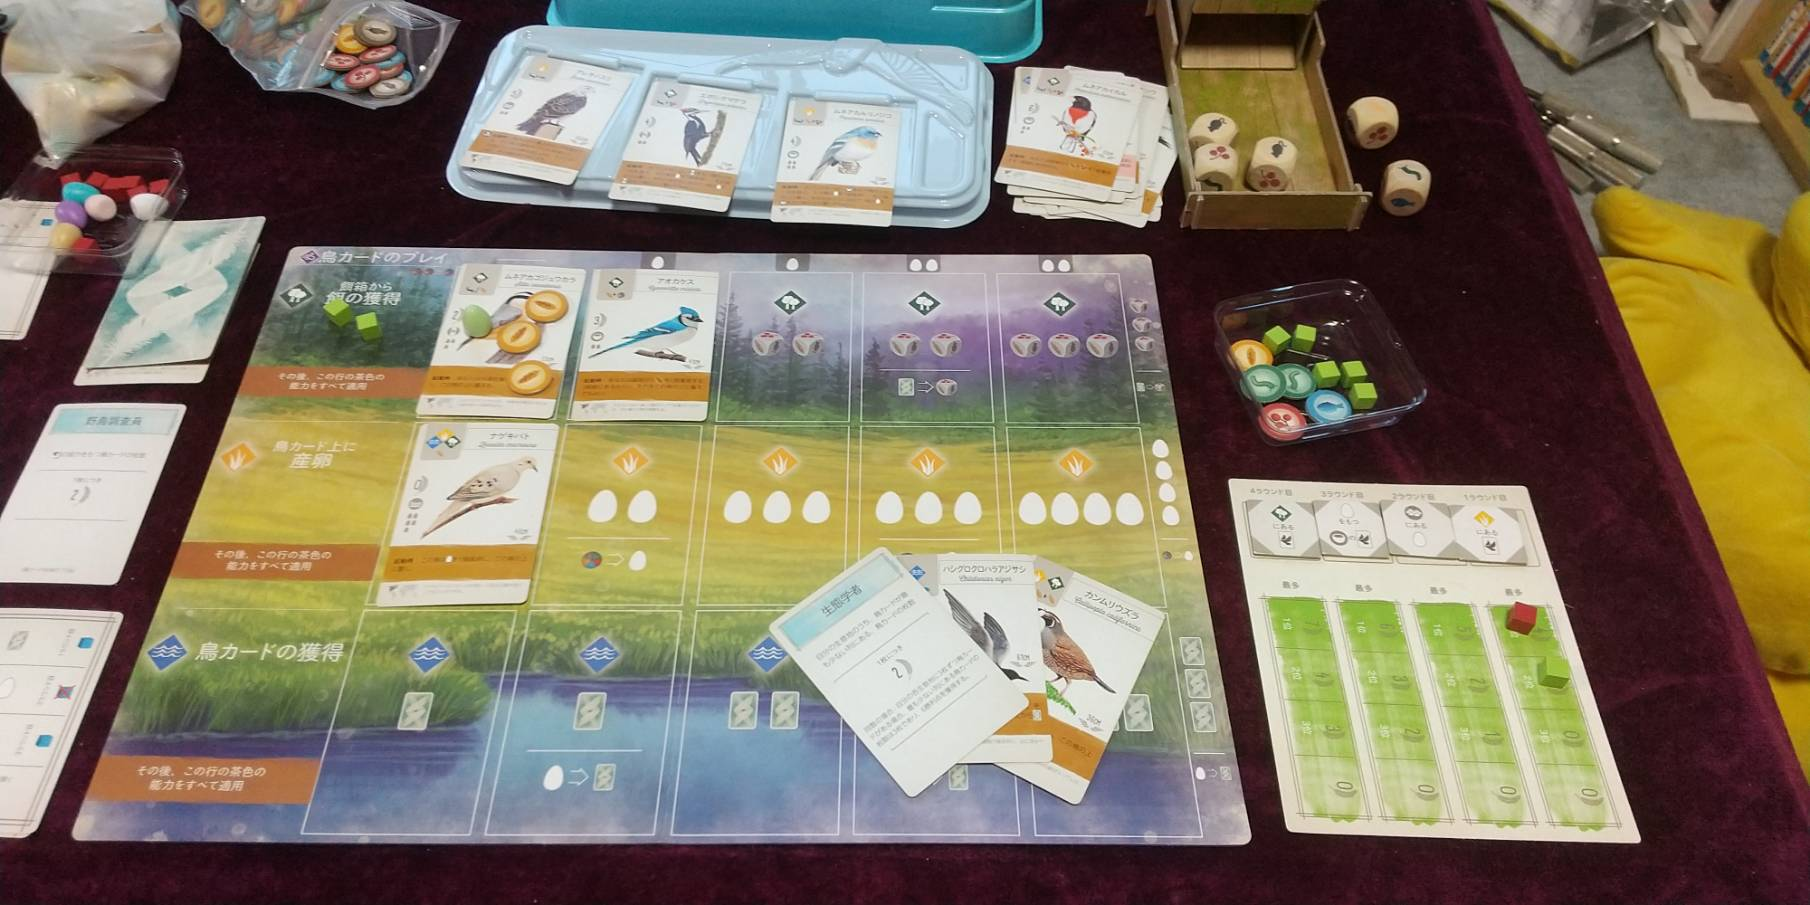
\includegraphics[height=7cm,width=15cm]{2025shinki/wing_span/real_play.jpg}
   \caption{実際にプレイしている様子}
   \label{fig:実際にプレイしている様子}
\end{figure*}
\par
餌の獲得を選択すると、一番上の行(森林)の空いているマスのうち最も左側に描かれたダイスの絵の数だけ餌トークンを獲得することができる。その際は、紙でできた餌箱の中にあるダイスを獲得する餌の数だけ外に移し、そのダイスの目が示している種類の餌を獲得する。餌箱からダイスがなくなった、あるいは餌箱にあるダイスの目がすべて同じときは、獲得する前にダイスをすべて振りなおすことができる。餌を獲得した後は、森林にプレイされている鳥カードの起動時能力を右端から順に発動させることができる。
\par
産卵を選択すると、二番目の行(草原)の空いているマスのうち最も左に描かれた卵の数だけ卵トークンを獲得し、プレイされている鳥カードが生むことができる卵の数を超えないように、好きな鳥カードの上に卵を置いていくことができる。産卵した後は、餌の獲得の時と同様に、草原にプレイされている鳥カードの起動時能力を右端から順に発動させることができる。
\par
鳥カードの獲得を選択すると、一番下の行(水辺)の空いているマスのうち最も左側に描かれた鳥カードの数だけ鳥カードを獲得することができる。この際、鳥カードは公開されている3枚の中から引くか、非公開にされている鳥の山の上から引くかを一枚ごとに選択することができる。公開されている3枚の中から引いた場合、引かれた分をトレイに補充するのはそのプレイヤーのターンが終わったときである。鳥カードを引いた後は、他の2つと同様に、水辺にプレイされている鳥カードの起動時能力を右端から順に発動させることができる。
\par
このようにゲームが進行していき、最終的には各プレイヤーごとに点数を計算していく。計算方法は、プレイされている鳥カードの得点の合計、ボーナスカードで得られた点数、ラウンド終了時目的から得られた点数、鳥カード上に産卵されている卵の総数、鳥カードの上に蓄えられている餌の総数、鳥カードに差し込まれている鳥カードの総数、の6項目の総和である。この総和が各プレイヤーの最終的な得点となり、その得点が大きい順に順位が決定していく。
\subsubsection{得点方法の分析}
ボードゲームの考察を行う際に最初にすべきことは、得点方法を整理することである。ウィングスパンにおいて、点数は以下の方法で得られる。
\begin{itemize}
  \item プレイした鳥カード
  \item ボーナスカード
  \item ラウンド終了時目的
  \item 卵
  \item 鳥の上に蓄えた餌
  \item 差し込んだ鳥カード
\end{itemize}
見方を変えれば、ウィングスパンはこの6通りの方法で得られた点数を競うゲームと言える。それぞれの項目で点数を増やすにはどうすればいいかを列挙すると、
\begin{itemize}
  \item プレイした鳥カード:鳥をたくさんプレイする。プレイするには「鳥カードを獲得→餌を獲得→(必要に応じて卵を獲得)→プレイ」
  という手順を踏む。
  \item ボーナスカード:条件を満たしている鳥をたくさんプレイする。
  \item ラウンド終了時目的:鳥をたくさんプレイするか、卵をたくさん産む。
  \item 卵:卵をたくさん産む。
  \item 鳥の上に蓄えた餌:鳥の能力をたくさん使う(やや特殊)
  \item 差し込んだ鳥カード:鳥の能力をたくさん使う(やや特殊)
\end{itemize}
という感じになる。基本的にはすべて鳥カードのプレイか産卵で賄えることが分かる。以上の得点方法と餌の獲得、鳥カードの獲得をまとめて、発展\footnote{本記事では、各生息地に鳥カードをプレイすることを、その生息地を「発展させる」と表現することがよくある。}の構造を図にすると図\ref{fig:発展構造}のようになる。
\begin{figure*}[htbp]
\begin{minipage}[b]{.5\textwidth}
  \centering
  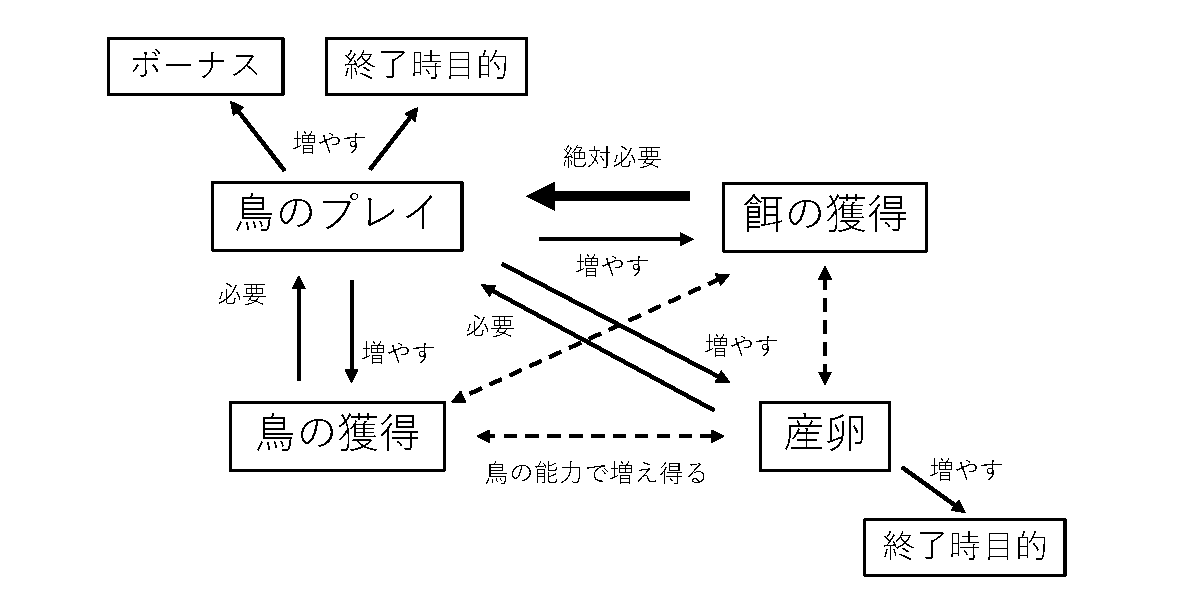
\includegraphics[height=4.2cm,width=8cm]{2025shinki/wing_span/WS_hattenkouzou.pdf}
  \caption{発展構造}
  \label{fig:発展構造}
\end{minipage}
\begin{minipage}[b]{.5\textwidth}
  \centering
  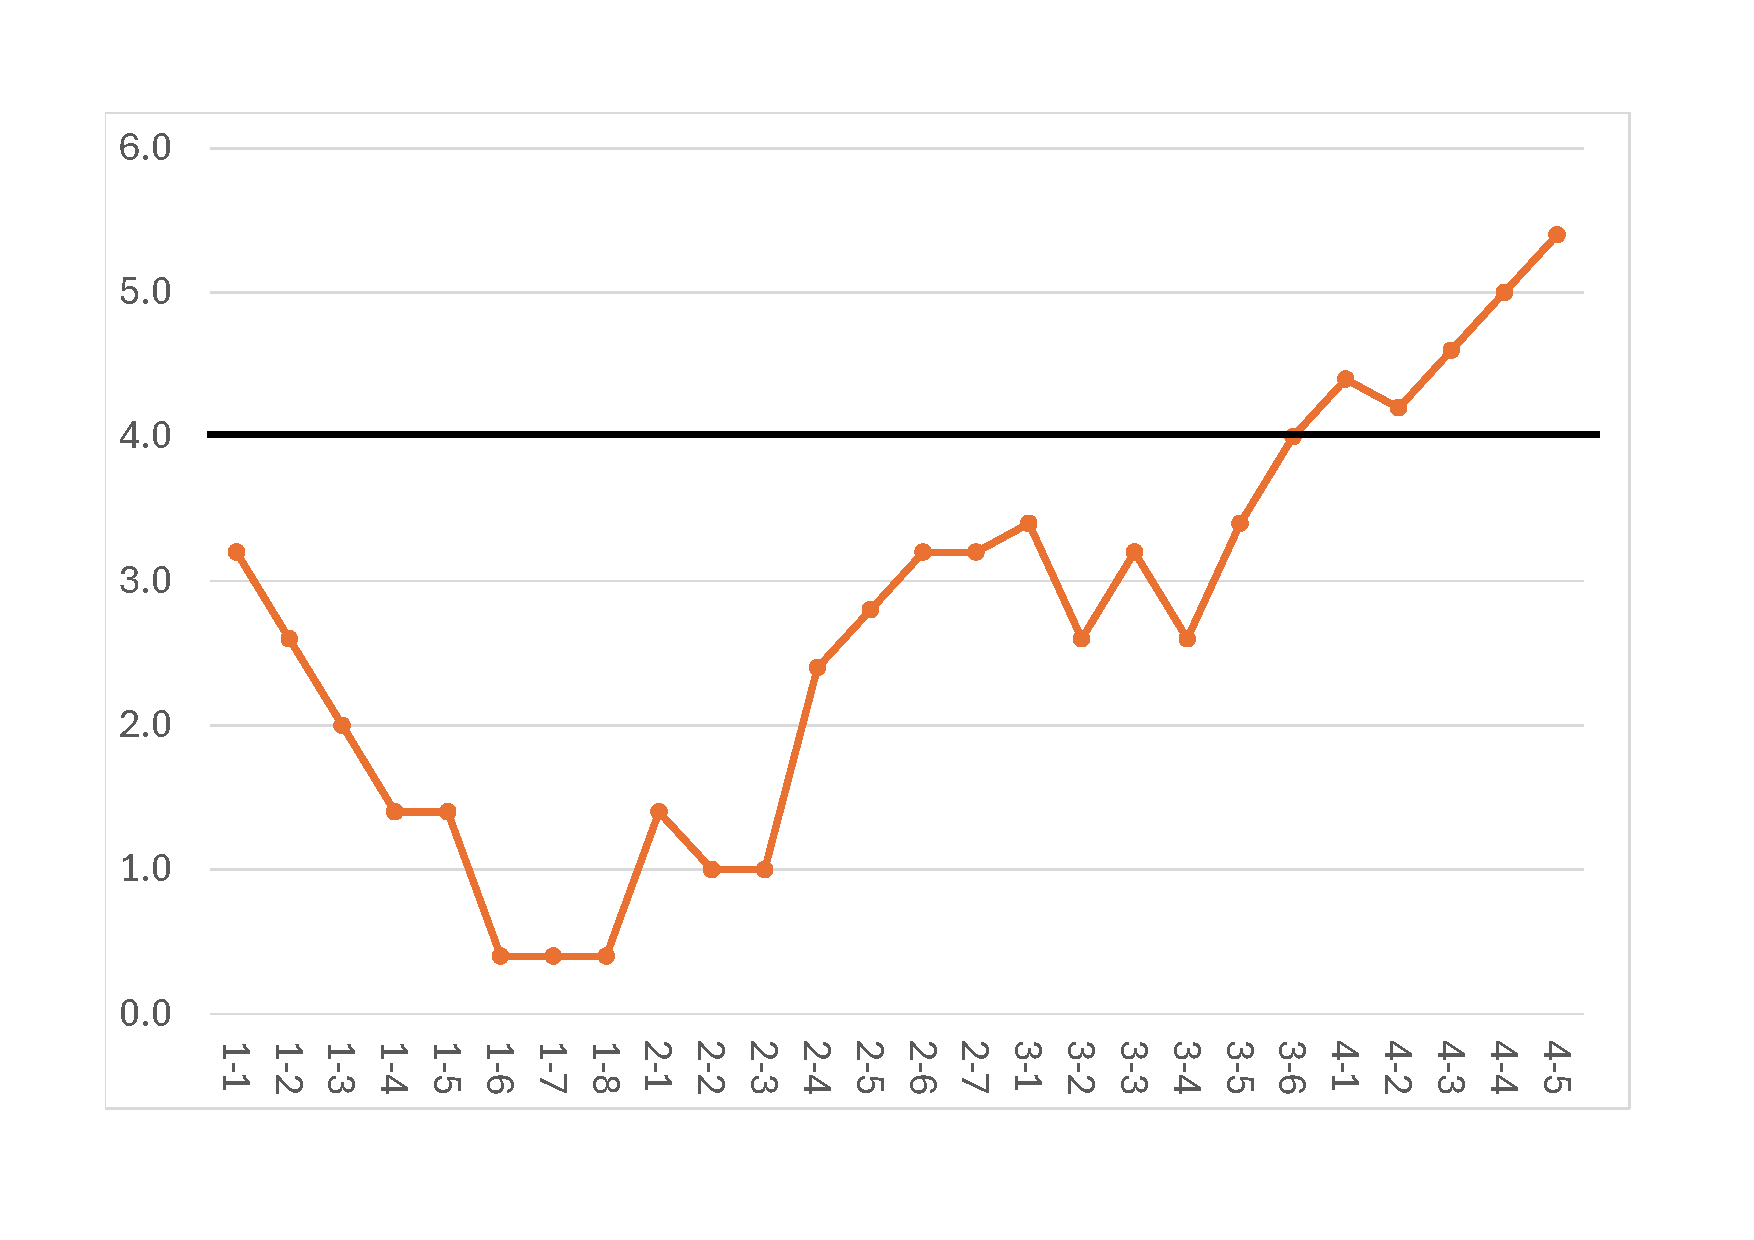
\includegraphics[height=5cm,width=7cm]{2025shinki/wing_span/WS_tokutennkouritu.pdf}
  \caption{ゲーム全体を通じた5ターンごとの得点効率の推移}
  \label{fig:得点効率}
\end{minipage}
\end{figure*}
この図における「絶対必要」と「必要」の違いは、使わなくても(あるいは行動しなくても)済むケースがあるか否かによる。餌コストは(必要ない鳥もあるが、鳥ごとの特徴を無視すれば)鳥をプレイする際には必ず必要になる。一方で卵は各生息地で1回目の発展では必要ない。また、鳥の獲得も1ターンで2枚獲得しておけば、2枚目をプレイする際にはわざわざもう一度鳥カードを獲得する必要はない。この意味で、卵と鳥カードの獲得は「今から鳥をプレイする」となったときに絶対必要だとは限らない。それゆえ、餌の獲得は鳥カードをプレイする上で他の2つよりも優先度が高い。
\par
先ほど述べたように、点数を得るには鳥のプレイと産卵という2通りの方法があった。産む卵の個数を増やすには鳥カードをたくさんプレイすればよい。よって、得点方法はすべて鳥カードのプレイに集約できる。そのうえで、プレイする鳥カードを増やすにはどうすればいいかを考えると、図\ref{fig:発展構造}より最も優先度が高いのは、獲得する餌の量を増やすことであると分かる。すなわち、ゲームが始まったら最初に森林に鳥カードをプレイして、餌の獲得量を増やすべであると言える\footnote{図\ref{fig:発展構造}で「鳥のプレイ」から矢印を逆にたどると「餌の獲得」と「鳥の獲得」がほぼ等価であることが分かる。実際、後で見るように森林の発展と水辺の発展はどちらを先にしても(つまり森林→水辺の順番で発展させても、水辺→森林の順番で発展させても)最終的な点数は理論上あまり変わらない。ただ、私の経験として森林を先に発展させた方が点数が発展するので、本記事では森林の発展の方にウェイトを置いている。なお、ラウンド終了時目的によってはこの限りではない。}。
\end{multicols}
\subsection{理想的な立ち回り}
\begin{multicols}{2}
\subsubsection{得点効率}
2章で述べたことから、ウィングスパンの理想的な立ち回りが導かれる。ただその前に、得点効率という指標について紹介しておく。後で述べる理想的な立ち回りは、この得点効率を最大化するものとして捉えれば理解が深まるからである。
\par
得点効率は以下の式で定義する。
\begin{equation}
  得点効率=\frac{得られる点数}{得点するために使ったターン数}\notag
\end{equation}
要するに1ターン当たり何点得られるかを意味しており、本記事ではゲーム全体を通してこれが最大になるような立ち回りについて論じているのである。
\par
ただこの指標には大域的なものと局所的なものがある。前者は全体を通して得点効率がいくつか、ということだ。例えば80点を取るには全体を通して得点効率が3点ちょっと必要になる。一方後者はある行動をして得点を得る際に、その行動の得点効率はいくつか、ということが問題になる。例えば、鳥カードを引いて、餌を獲得して、鳥カードをプレイする、という一連の流れには原則として3ターンかかる。すると、鳥の得点は高々9点であるから、鳥カードをプレイする操作の得点効率は最大でも3であると言える。いちいち名前を分けるのは面倒くさいので本記事では文脈に応じて意味を使い分けるが、なるべく分かりやすいように書くつもりである。
\par
またここで挙げた例からも分かるとおり、80点をとるには鳥カードをプレイしているだけでは届きそうにない。それゆえ、もっと得点効率の高い(これはどちらかと言えば局所的な意味で)行動をすべきなのである。
\par
実戦において得点効率がどのように推移しているかを見てみよう。図\ref{fig:得点効率}は、私が実際にオートマ戦での操作から5ターンごとの追加点の移動平均を得点効率として割り出して描いたものである。ただし、このグラフではラウンド終了時目的とボーナスカードについては考慮していないことに注意されたい。
\par
グラフの横軸にある数字はラウンドとターンを表している。例えば、1-1は1ラウンド目の1ターン目ということになる。また、最初の2つと最後の2つの値に関しては、端のデータに重きが置かれるように計算した。例えば、1-1の値$a_{1-1}$と1-2の値$a_{1-2}$は$i-j$のデータ$x_{i-j}$を用いて以下の式で表される。
\begin{gather*}
  a_{1-1}=\frac{x_{1-1}+x_{1-1}+x_{1-1}+x_{1-2}+x_{1-3}}{5}\\
  a_{1-2}=\frac{x_{1-1}+x_{1-1}+x_{1-2}+x_{1-3}+x_{1-4}}{5}
\end{gather*}
$a_{4-4}$と$a_{4-5}$も同様である。
\par
このグラフを見て分かるように、局所的な得点効率ははじめは高く、途中に下がったのちに最後にもっとも高くなることが分かる。特に、4ラウンド目には毎ターン4を超えている。この例に限らず、多くのゲームにおいてこの傾向はみられる。この時の最終的な得点は85点であった。鳥をプレイするだけでは得点効率は高々3であったが、最後に得点効率が4を超えたことがプラスに作用したと言えよう。この要因は4ラウンド目のほとんどを産卵に費やしたことである。次節で詳しく述べるが、産卵アクションは最も得点効率が高くなりやすい。それゆえ、4ラウンド目に産卵アクションで回収できる得点ができる限り高くなるように草原に鳥を配置しておくことが肝要なのである。
\subsubsection{理想的な立ち回り}
前節で述べたことを踏まえ、理想的な立ち回りを導く。まず大前提として、得点効率が最も高くなり得るのは産卵である。草原に4枚鳥をプレイしておけばそれだけで1ターンあたり4点は得られるし、それに鳥の能力を加えれば1,2点追加される。運が良ければ1ターンに6点得ることも可能になるのだ。それゆえゲーム全体の目標は4ラウンドに入る前に草原に4枚以上の鳥カードをプレイして、得点するシステムを構築することなのである。
\par
どのようなシステムを構築するかは持っている鳥カードを見て決めるため、草原の開発は最後になる。それまでは森林と水辺を開発することになる。ここでもプレイ時の卵の消費量を考えて3羽プレイすることを目指す。具体的には、まず森林と水辺の両方に2枚鳥をプレイして鳥と餌の供給ラインを作る\footnote{2羽以上プレイすれば、もらえる餌の量や鳥カードの枚数が1つから2つに増える。1ターンで餌が2つ得られれば、2コストの鳥の餌が1ターンでそろうことになる。}。その後、余裕ができたら3枚目をプレイする、という形が理想的である。
\par
以上のようなことを踏まえ、以下のような立ち回りを提唱する。以下、この立ち回りを「理想的な立ち回り」と呼ぶことにする。
\begin{align*}
  &\textbf{1-1} &&森林に鳥カードをプレイ\\
  &\textbf{1-2} &&産卵(2個)\\
  &\textbf{1-3} &&森林に鳥カードをプレイ(卵-1)\\
  &\textbf{1-4} &&鳥カードを獲得(1枚)\\
  &\textbf{1-5} &&餌を獲得(2個)\\
  &\textbf{1-6} &&水辺に鳥カードをプレイ\\
  &\textbf{1-7} &&鳥カードを獲得(1枚)\\
  &\textbf{1-8} &&餌を獲得(2個)\\
  & \tiny{ } && \\
  &\textbf{2-1} &&水辺に鳥カードをプレイ(卵-1)\\
  &\textbf{2-2} &&鳥カードを獲得(2枚)\\
  &\textbf{2-3} &&鳥カードを獲得(2枚)\\
  &\textbf{2-4} &&産卵(2個)\\
  &\textbf{2-5} &&餌を獲得(2個)\\
  &\textbf{2-6} &&草原に鳥カードをプレイ\\
  &\textbf{2-7} &&餌を獲得(2個)\\
  & \tiny{ } && \\
  &\textbf{3-1} &&草原に鳥カードをプレイ(卵-1)\\
  &\textbf{3-2} &&餌を獲得(2個)\\
  &\textbf{3-3} &&草原に鳥カードをプレイ(卵-1)\\
  &\textbf{3-4} &&餌を獲得(2個)\\
  &\textbf{3-5} &&産卵(3個)\\
  &\textbf{3-6} &&草原に鳥カードをプレイ(卵-2)\\
  & \tiny{ } && \\
  &\textbf{4-1} &&産卵(4個)\\
  &\textbf{4-2} &&産卵(4個)\\
  &\textbf{4-3} &&産卵(4個)\\
  &\textbf{4-4} &&産卵(4個)\\
  &\textbf{4-5} &&産卵(4個)\\
\end{align*}
これについてラウンドごとに意味を説明していく。
\par
まず1-1~2-1では、森林と水辺に2枚ずつ鳥カードをプレイするのが目標である。最初に手元に残す鳥を選ぶ段階では鳥の得点や起動時能力よりも餌コストを重視し、開始3ターンで森林に2枚鳥カードをプレイできるようにするのが原則だ。そのために、最初に配られた5枚の鳥カードから手元に残すカードは、必要な餌コストの合計が3で、必要な餌が被っておらず、かつともに森林に生息するような2枚とするのが基本となる。森林を整備した後は水辺の鳥を引き、できるだけ2-1までに水辺にも2枚鳥カードをプレイするようにしたい。また、このフェーズではあまりラウンド終了時目的を取りに行くべきではない。取りに行っても高々4点しか変わらないため、これから先の得点効率を落としてまで取りに行くべきではない。理想的な立ち回り通りにプレイしていたらとれていた、という状況が望ましい。
\par
その後2-2~2-7にかけては草原にプレイする鳥カードを集めるフェーズとなる。できるだけ産卵した時にもう1点取れる鳥カードを集めるようにする。ただ、それだけだとターン数が余ってしまうので、一度鳥をプレイする部分を作ってある。ラウンド終了時目的は取れなさそうなら諦めるべきである。鳥を集める際にボーナスカードの条件も考慮するのは忘れないようにする。
\par
3ラウンド目は、2-2~2-7にかけて集めた鳥をひたすらプレイするフェーズである。ラウンド終了時目的もとれるように鳥を集めておくのがコツである。終了時目的とボーナスカードを絡めるのは少し難しいが、うまくできるとだいぶ得点が安定するようになる。なお、この理想的な立ち回り通りにできない場合は、3ラウンド目の後半に一度時間をとってどうするのが最も得点効率がいいか考えて、それ以降の立ち回りを決めるのを推奨する。終盤になれば、どうするのが最終的にもっとも高得点になるのか計算できるようになるからだ。
\par
最終ラウンドはひたすら産卵するフェーズである。鳥が蓄えられる卵の平均値は2.85個(小数点第3位以下四捨五入)、最頻値は2個(いずれも実際に数えたが、詳細は紙面の都合上割愛)であるから、全体で16~22個程度産卵することができる。このラウンドは最も1ターン当たりの得点効率が高くなる部分であるから、ひたすら産卵を繰り返す。
\par
理想的な立ち回りでは鳥カードで35~40点、ボーナスカードで3~8点、ラウンド終了時目的で10~15点、卵の個数と蓄えた餌の数、差し込んだ鳥カードの枚数をすべて合わせて30~40点の計80~90点程度とれる。もちろん運が良ければ上振れるし、悪ければ80点に届かないこともある。ただ、本記事では以後この立ち回りをモデルケースとして細部を肉付けていきたい。
\subsubsection{例外}
上で述べた理想的な立ち回りはあくまで理想的なもので、様々な仮定の下に実現可能なものである。上の立ち回りができるための条件は、以下の3つである。
\begin{itemize}
  \item 最初に餌コストが1個と2個(しかも被りがない)で森林に生息する2枚の鳥カードがあること
  \item 1-4や1-7で水辺に生息する鳥を引けること
  \item 2ラウンド目で1点稼げる起動時能力を持っており、かつ草原に生息する鳥を引けること
\end{itemize}
これらの条件がそろわない場合は、理想的な立ち回りは実行できない。それゆえ、別途立ち回りのパターンを組む必要がある。上の条件が満たされない場合やパターンでは想定されていないラッキーやアンラッキー(主にアンラッキーの方)を、本記事では「例外」と呼ぶことにする。理想的な立ち回りで生じる例外は、大きく分けて以下の5つだ。
\begin{enumerate}
  \item 最初に4ラウンド目に使える鳥を引いた場合
  \item 最初に森林に生息する鳥を満足に引けなかった場合
  \item 1-4や1-7で水辺に生息する鳥カードが引けなかった場合
  \item 2ラウンド目で1点稼げて草原に生息する鳥カードを引けなかった場合
  \item 2,3ラウンド目で点数の低い鳥カードしか引けなかった場合
\end{enumerate}
これらの例外に対して、次章で対処法を見出していく。紙面の都合上、(i)と(i\hspace{-1.2pt}i\hspace{-1.2pt}i)の2つについてのみ処理する。
\end{multicols}
\subsection{例外処理}
\begin{multicols}{2}
\subsubsection{処理すべき例外と処理しなくてもよい例外}
発生し得る例外をすべて考慮していては途方もなくなってしまう。例えば、最初からずっと草原にしか生息しない鳥カードしか引けないことは理論上あり得るが、起こる確率はとても低い。本記事ではこのような例外に対してもいちいち対処法を考えることはせず、起こったら運の悪さを嘆いて諦める、という立場をとることにする。それゆえ、例外処理に移る前にまず考慮する例外と考慮しない例外について述べておく。
\par
単刀直入に、本記事では発生確率\footnote{ただし、ここでいう発生確率とは条件付き確率のこととは限らないことに注意されたい。条件付き確率を求めている際は、その旨をしっかりと明記している。}が100分の1未満の例外については考慮しない。すなわち、100回に1度も起こり得ないケースが起こった場合は諦める、という立場をとる。例えばある例外を処理していく中で、ここから先のケースは発生確率が100分の1未満だからその手前までで例外は処理されている、というようにして処理を進めていく。このようにしてすべての場合がつくせたら、例外処理完了、ということになる。なお、本記事は全体を通してオートマ戦が基準になっているため、確率計算も次の自分の手番までに鳥カードが1枚も引かれなかったうえでの確率を求めている(これはオートマ戦でも起こることがない、かなり理想的な状況である)。ただ、例外が起こる確率を求める際は、基本的にはカードが引かれていない方が確率が高くなるので、より多くの例外を処理する必要があると考えればそこまで気にする必要はない。

\subsubsection{例外処理(i) 最初に4ラウンド目以降に使える鳥を引いた場合}
この例外は、理想的な立ち回りにおいては2ラウンド目に欲しい鳥が最初に配られた5枚の鳥の中にあった場合を意味している。例えば卵を1個産む起動時能力を持った鳥(そして、このような鳥はたいてい草原にしか生息しない)が最初に配られたカードにあった場合などがこれにあたる。結論から言えば、森林か水辺に生息していない限りそのようなカードは最初に捨ててもよい。なぜならば、起動時能力で1点稼げる鳥カードは2ラウンド目に引けばよいのであって、最初に引けたからといってそこに執着していては餌や鳥カードの供給ラインを整備することもままならなくなり、本末転倒だからである。最初に意識すべきは森林と水辺に2枚ずつ鳥カードをプレイすることであって、起動時能力で1点稼げる鳥を引くことではない。捨てるのはもったいないかもしれないが、またあとで巡り合えると信じて一旦手放すのが最善手になる。ただ、森林や水辺に生息する鳥カードが引けなかった場合や引けても1枚程度だった場合はその限りではない。その場合は例外(i\hspace{-1.2pt}i)に相当するが、これについては本記事では扱わない。
\subsubsection{例外処理(i\hspace{-1.2pt}i\hspace{-1.2pt}i) 1-4や1-7で水辺に生息する鳥カードが引けなかった場合}
まずはこの例外が発生する確率を求める。前提としてこの例外は初めに配られた鳥カードに森林に生息する鳥が十分にあった場合に発生するものであるから、欲しいのはそのうえで水辺に生息する鳥カードを引けない条件付き確率である。さらに、その条件付確率が最も大きくなるのは、初めに水辺に生息する鳥カードのみを引いたときである。よって、水辺に生息する鳥カードは計85枚あるので、この例外が起こる条件付き確率は最大で
\begin{equation*}
  \frac{{}_{85} \mathrm{C}_3}{{}_{165} \mathrm{C}_3}\times\frac{82}{162}\times\frac{81}{161}=0.0342\cdots>0.01
\end{equation*}
となる。よってこの例外が発生する確率は高々0.034(30回に1回程度)と言える。低いが、0.01を超えてはいるので、一応処理を検討しておく。一方で上の状態からもう1回カードを引いても水辺に住む鳥を引けない確率は、
\begin{equation*}
  \frac{{}_{85} \mathrm{C}_3}{{}_{165} \mathrm{C}_3}\times\frac{82}{162}\times\frac{81}{161}\times\frac{80}{160}=0.0171\cdots>0.01
\end{equation*}
であり、ここからもう1回カードを引くと、水辺に住む鳥カードが得られない確率が0.01を下回る。よって、3回鳥カードを引いても水辺に住む鳥を獲得できない場合に対して処理を与えればよい。
\par
理想的な立ち回りにおいて、1-4以降3回鳥カードを引いても水辺に住む鳥を引けなかったという体で、それ以降の立ち回りを組む。1例として、以下のような立ち回りを提唱する。

\begin{align*}
  &\textbf{1-1} &&森林に鳥カードをプレイ\\
  &\textbf{1-2} &&産卵(2個)\\
  &\textbf{1-3} &&森林に鳥カードをプレイ(卵-1)\\
  &\textbf{1-4} &&鳥カードを獲得(1枚)\\
  &\textbf{1-5} &&餌を獲得(2個)\\
  &\textbf{1-6} &&草原に鳥カードをプレイ\\
  &\textbf{1-7} &&鳥カードを獲得(1枚)\\
  &\textbf{1-8} &&餌を獲得(2個)\\
  & \tiny{ } && \\
  \displaybreak
  &\textbf{2-1} &&草原に鳥カードをプレイ(卵-1)\\
  &\textbf{2-2} &&鳥カードを獲得(1枚)\\
  &\textbf{2-3} &&餌を獲得(2個)\\
  &\textbf{2-4} &&産卵(3個)\\
  &\textbf{2-5} &&草原に鳥カードをプレイ(卵-1)\\
  &\textbf{2-6} &&鳥カードを獲得(1枚)\\
  &\textbf{2-7} &&餌を獲得(2個)\\
  & \tiny{ } && \\
  &\textbf{3-1} &&草原に鳥カードをプレイ(卵-2)\\
  &\textbf{3-2} &&鳥カードを獲得(1枚)\\
  &\textbf{3-3} &&餌を獲得(2個)\\
  &\textbf{3-4} &&水辺に鳥カードをプレイ\\
  &\textbf{3-5} &&鳥カードを獲得(1枚)\\
  &\textbf{3-6} &&餌を獲得(2個)\\
  & \tiny{ } && \\
  &\textbf{4-1} &&産卵(4個)\\
  &\textbf{4-2} &&水辺に鳥カードをプレイ(卵-1)\\
  &\textbf{4-3} &&産卵(4個)\\
  &\textbf{4-4} &&産卵(4個)\\
  &\textbf{4-5} &&産卵(4個)\\
\end{align*}
これについても順を追って説明する。
\par
まず1-3までは理想的な立ち回り通りである。1-4以降は、水辺に生息する鳥カードが得られないので、草原に住む鳥カードを引く\footnote{この時に鳥の山から引いて森林にしか生息しない鳥カードを引いても後の立ち回りはさほど変わらない。草原の列にプレイされている鳥カードが1枚減って、森林の列にプレイされている鳥カードが1枚増えるだけである。この場合は産む卵が少なくなる分70点ぐらいが標準だと思われる。}。しばらく「草原にすむ鳥カードを引く→餌を獲得→(必要なら産卵→)鳥カードのプレイ」という流れを繰り返し、草原に4枚の鳥カードをプレイしておく。そうすると、1回で4個の卵を産めるようになる。それから3ラウンド終了までの余ったターンは、森林か水辺にすむ鳥カードを引き、順にプレイしていって鳥カードの点数を稼ぐ。最後の4ラウンド目では、3-5で引いた鳥カードを途中でプレイするほかは毎ターン4個ずつ卵を産んでいって得点を稼ぐ。
\par
この立ち回りでは鳥カードの得点32点、ボーナスカード3,4点、ラウンド終了時目的10点、卵15個、蓄えた餌の個数と差し込んだ鳥カードの点数が合わせて10点の合計70点程度が期待できる。もちろん早い段階で卵を産む起動時能力を持った鳥をプレイできれば、4-1でもう1羽鳥をプレイしてもう少し点数を伸ばすこともできる。ギリギリ80点には届いていないが、ここまで起こり得ないアンラッキーな例外で70点取れるなら上出来だろう。
\par
この立ち回りの肝は、プレイする鳥カードの枚数を増やせない分を、産む卵の個数を増やすことで補填するという点である。そのために草原に4枚以上の鳥カードをプレイすることが望ましい。ただ、基本的には多くの鳥カードを引けなければプレイの選択肢が狭まり、鳥の得点はおろかボーナスカードや終了時目的での得点も難しくなるので、80点をとるのはなかなか厳しい\footnote{この点を考慮すると最初に発展させるのは水辺の方がいいような気もしてくるが、うまく水辺に鳥カードをプレイできたとしても、多くの場合餌がなかなかそろわないのでなかなかゲームが進まない。最初の2ターンで森林と水辺に1枚ずつプレイしておくというのもアリだが、それも餌ガチャと鳥カードガチャの両方に足を突っ込むことになり、微妙な気もする。}。
\par
以上で例外(i\hspace{-1.2pt}i\hspace{-1.2pt}i)は解決された。
\end{multicols}
\subsection{おわりに}
\begin{multicols}{2}
本記事では、最初にウィングスパンのルール分析から発展構造を図におこし、それを用いて理想的な立ち回りを導いた。ただこの立ち回りはあくまで理想的なものであって、様々な都合の良い仮定のもとに成り立っている。そこで、そうした仮定が成り立たない場合を例外として列挙し、対処法を模索した。具体的には、発生確率が0.01未満のものに関しては考慮すべきものではないとして切り捨て、それ以外のものに対しては、理想的な立ち回りと比べて得点効率が下がり得るのか検討した。下がり得ないものは理想的な立ち回りを柔軟に変えて対処し、下がり得るものは、そのケースでも80点近くとれるような代替の立ち回りを提唱した。
\par
本記事を通してウィングスパンの定石というものがある程度確認されたのではないかと私は考えている。まず1ラウンド目で森林と水辺に2枚の鳥カードをプレイし、2ラウンド目で草原にプレイする鳥カードを収集し、3ラウンド目にそれらの鳥カードをプレイし、最後の4ラウンド目でひたすら産卵して得点を稼ぐ、という、安定して点数を得るための機械的な立ち回りが一つ得られた。実践では、これをもとにボーナスカードやラウンド終了時目的を考慮して臨機応変に対応すればよい。想定していなかった例外が発生しても、できる限りどこかで理想的な立ち回りと合流できるような手を打っていけばいい。
\par
また、定石を導いたのみならず、導き方のアウトラインを与えたことも、本記事における成果の一つである。ウィングスパンのような発展構造がループしているボードゲームに関しては、その構造を整理すれば、一番最初に手を付けるべきところが定まる。そこからゲームの得点しどころを見極め、そこでの得点効率を最大化するように手順を整備すれば、それが一つの定石になるというわけである。本記事で私がとった手法を応用していけば、似たような性質を持つ他のゲームについても容易に定石を構築できるようになるはずである。
\par
一方で、本記事では解決できなかったこともいくつかある。まず挙げられるのは、拡張版で遊ぶ際にはどうすればいいか、という問いである。本記事で扱ったのは無印のウィングスパンであるが、2024年現在、ウィングスパンには他にも欧州、大洋、東洋、という3つの拡張版があり、これらには新しい鳥に加え、無印にはなかった終了時目的、能力などが加わり、よりゲームを複雑にしている。それらについても今後分析していく必要がある。また、より細かい点を挙げれば、私はまだ以下のことが分かっていない。
\begin{itemize}
  \item ボーナスカードやラウンド終了時目的の活かし方
  \item 鳥の能力の詳細な分類と、能力の活用法
  \item 常に最善手を打った際にとり得る点数の分布
  \item 対人戦におけるインタラクションについて\footnote{まぁ一緒に研究してくれる人がいないので調べられないのだが。}
\end{itemize}
こうしたことはウィングスパンを完全に理解するためには知っておく必要があるため、今後の研究で取り組むべき課題であろう。本記事をきっかけにして、ウィングスパンはもちろんのことより多くのボドゲの定石研究が盛んになれば、それは筆舌に尽くしがたい幸福である。
\par
ここまで非常に長くなったが、最後に。私がウィングスパンを研究し始めた当初は、鳥カードは餌コストと得点、産む卵の個数、能力を対応させる記号にしか見えなかった。きっかけとなった耐久ボドゲ会でも、他の2人が鳥カードを愛でているそばで「かわいいのは分からなくはないんだけどなあ...」と、いまいち腑に落ちない気持ちであった。しかし、研究のためにオートマ戦を繰り返す中で、ふと鳥カードをかわいいと思う瞬間があった。その時を境に私は遊びながら鳥を愛でることを覚え、かくして2人、そしてウィングスパンを遊ぶ他の談話室民たちの仲間入りをしたのである。
\par
私の推しは「アオバネアメリカムシクイ」、「クロズキンアメリカムシクイ」、「オウゴンアメリカムシクイ」、「ミズイロアメリカムシクイ」の4羽である。
\end{multicols}
\begin{figure}[h]
\centering
\begin{minipage}[b]{0.23\columnwidth}
    \centering
    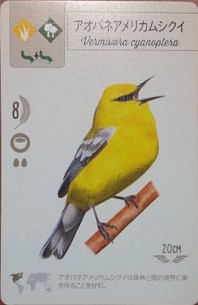
\includegraphics[width=0.9\columnwidth]{2025shinki/wing_span/aobaneamerikamusikui.jpg}
    \caption{アオバネアメリカムシクイ}
    \label{fig:アオバネアメリカムシクイ}
\end{minipage}
\begin{minipage}[b]{0.23\columnwidth}
    \centering
    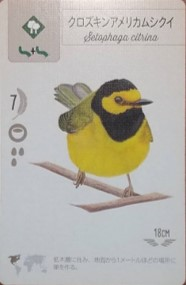
\includegraphics[width=0.9\columnwidth]{2025shinki/wing_span/kurozukinnamerikamusikui.jpg}
    \caption{クロズキンアメリカムシクイ}
    \label{fig:クロズキンアメリカムシクイ}
\end{minipage}
\begin{minipage}[b]{0.23\columnwidth}
    \centering
    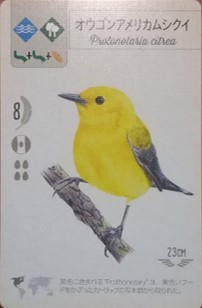
\includegraphics[width=0.9\columnwidth]{2025shinki/wing_span/ougonamerikamusikui.jpg}
    \caption{オウゴンアメリカムシクイ}
    \label{fig:オウゴンアメリカムシクイ}
\end{minipage}
\begin{minipage}[b]{0.23\columnwidth}
  \centering
  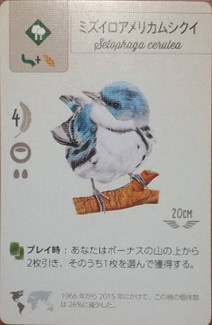
\includegraphics[width=0.9\columnwidth]{2025shinki/wing_span/mizuiroamerikamusikui.jpg}
  \caption{ミズイロアメリカムシクイ}
  \label{fig:ミズイロアメリカムシクイ}
\end{minipage}
\end{figure}
\begin{multicols}{2}
\par
やはり何と言っても絵柄がかわいい。ぬいぐるみにしたらやや小太りでふさふさの毛並みをしていそうで愛くるしい。抱きかかえて頭をなでなでしたくなる。しかも鳥効率が高いものばかりで強いところもいいし、翼長が短いのでハヤブサなどの起動時能力で引いたときも残念な気分にならない。それどころか、少し可哀そうな気分にさえなる。なにせ捕食者の能力で食べられちゃうので。
\par
推し鳥ができてから、私のウィングスパンは格段に幸せなものになった。カードを引いてゲットできたらうれしくなるし、鳥の山から3枚とって公開した時に見えた際にはすぐに取りに行く(実際強いから別に悪手ではない)。相手にとられると悲しくもなる。こんなかわいい鳥たちがいるウィングスパンを買ってきてくれた現&元談話室民には非常に感謝しているし、私が廃れるきっかけを作ってくれた同期のボドゲ民たちには頭が上がらない。
\end{multicols}

  
  \newpage
  \section{出張版 C12 談話室 on web 「とある日のこと」}
  
  

\setlength{\parskip}{1em}
\setlength{\parindent}{0pt} 

\newtcolorbox{myboxnote}[1][]{%
  breakable           % ページを跨げるようにする
}


\begin{center}
    \Large\textbf{出張版C12談話室 on web 「とある日のこと」}\\
    \vspace{1em}
    \text{文責 : C12有志}
\end{center}

\vspace{1em}

\subsection{「とある日のこと」とは}
\noindent
 入寮パンフレットをパラパラと眺めているあなたの関心は、つまるところ「熊野寮にはどんな人が住んでいて、どのように暮らしているのか」にあるのではないでしょうか。\\
 本企画は、C12に住む寮生8名の、ある日の日記を集めたものです。切り出された出来事からはそれぞれの暮らしが、エピソードの選び方や筆致からはそれぞれの人柄が、ほのかに見えてくることと思います。\\
 人の数だけある生活、その断片を覗いてみてください。\\

\vspace{1em}
\begin{myboxnote}
\subsection{冬も愛おしく思えた一日}
\noindent
12月15日、12時半。昨日は部活の追いコンで朝まで飲んでいたため、当たり前のように昼に起きた。寒くて外に出る気力もないので、寮の食堂で卒論を書く。少し作業した後、談話室に寄ると、同じく食事中の同期Mがコタツに刺さっていた。C12談話室では最近テレビが解禁されて、日本のスナック文化について研究する外国人博士という、興味深い番組が流れていた。2人で「面白かったねー」なんて言いながら談話室を後にした。その後も引き続き作業を進め、今日は第1章の下書きができあがった。また談話室に戻って夕食を食べていると、先輩Aと後輩Sからパスタをおすそ分けしてもらうなどした。寮の委員会の仕事をして、風呂に入り、22時からブロック会議だった。長い会議が終わって、後輩Sの誘いに乗り、同期Mも一緒にファミマまで行って、2人でおでんを選んだ。談話室に帰って、駄弁ったり作業したりなんかしてると、車でラーメンに行ったはずの4人が早々に帰ってきた。墓地に迷い込んで、断念しちゃったんだって。私はというものの、おでんで大根とはんぺんしか食べなかったためお腹が空いて困っていた。これはちょうど良いと、ラーメンを食べ損ねて少ししょんぼりしている後輩Aをコンビニに誘った。コンビニの2往復なんて冷静に考えればしょうもないムーブのはずだけど、あの100mぐらいの道のりを、こうやって人と話しながら、あったかい食べ物を抱えて、てくてくと歩けるこの時間を今日はすごく幸せに思った。コンビニのおでんもかつ丼も、昔はしょっぱくて好みじゃなかったはずなのに、今ではすっかり慣れてしまった。それはきっと、寮生活で身に付いた一種の堕落であると同時に、みんなと過ごしてきた時間の積み重ねなんだと思う。ご飯もたくさん食べちゃったし、みんながゲームに興じてる姿を横目に見ながら、夜更かししようかな。真冬のコタツと談話室は、今日もほっこりとあたたかい。\\

\noindent
\textbf{うの}\\
総合人間学部4回生。1回生入寮。趣味は寮でのバンド活動(歌、ギター、ピアノ)。体育会サイクリング部所属。談話室では主に皆と話したり、バンドの練習をしています。

\vspace{1em}

\end{myboxnote}

\begin{myboxnote}
\subsection{241127 : よくものを失くす}
\noindent
 今日は無くしたものを拾ったと思ったら別の無くしたものに気がつく、そんな一日だった。\\
 先日、音源や過去に作成した楽曲のプロジェクトファイルがどかっと詰まった2TBのSSDを無くした。慌てふためくも用事のために泣く泣く電車に乗って数日間寮を空けていたが、この昼に自室に戻って机の下を探すと床に転がっていた。こんなところにいたのか。\\
 陽も暮れて夕方、C12の面々と紅葉を観に御所へと出かけた。正直なところ暗くてよく分からなかったが、わいわい出かけられたらそれで十分楽しいものだ、なんて思っていたら、寮に戻って一行で寮食をとろうという時に財布がないことに気がついた。一人でそそくさと輪を抜け、談話室や部屋を探すが見当たらない。血の気が引く。先ほどのお出かけで落としてしまったのかもしれない。\\
 小雨の降る中、一人で寒い道を歩く。スマホのライトを最大まで明るくし、見落としがないように注意深く探す。このときだけは御所のだだっ広さが憎かった。勝手な話だ。\\
 結局来るとこまで来てしまった。あとは帰り道を丹念に探すしかない。渋々交番に遺失届を出そうかと思ったが、その前にC12のラインで財布を無くした報告をすることにした。すると2分後、先輩が見つかったよとの連絡を下さった。もっと早めにSOSを出していたらこの無駄足はなかったかもとは思ったが、とにかく見つかったことにほっとした。\\
 寮に戻り、拾ってくれた人にお礼を言って財布を受け取り、寮食をとった。美味しかった。\\
 体を流して寝る準備をしようとシャワー室に行くと、今度はシャワーカードがなくなっていることに気がついた。冷や汗をかきながら事務室の落とし物入れを探していると、そこには見覚えのある私のシャワーカードが入っていた。胸を撫で下ろした。\\
 風呂上がり。乾燥が気になる季節だが化粧水も乳液もバイト先に忘れてしまった。シフトまでまだ日があるし、職場までは微妙に距離があって用事もなく行くのは面倒なので、その間はみっともなくバキバキな肌をマスクでなんとか隠していくことになりそうだ。あーあ。\\
 
\vspace{1mm}
\noindent
\textbf{白橋つむぐ}\\
音楽系の高校をフルート専攻生として卒業。今は経済学部で社会思想史を専攻している。

\end{myboxnote}
\vspace{1em}

\begin{myboxnote}
\subsection{訳ありレモン}
\noindent
 なんだか今日は息苦しい一日だった。無理に体をベッドから起こして、何のあてもなく徒歩一分のファミリーマートへ向かう。不穏な灰色の雲が、いつもよりも近くにある気がした。\\
 僕は閉塞感でいっぱいになっていた。自分も周りもすべて行き詰っているように思えてならず、何をしてもニヒリズムに陥りそうだった。逃げ出すように何かしたい、どこかに行きたいと一念発起するけれど、そんな元気なんてないぞ、と心の中の何かが言うとその決心は急速に萎んでしまうのだった。\\
 歩きながらふと、梶井基次郎の『檸檬』を思い出した。そういえば彼も晴れない憂鬱に頭を悩ませていたな、と妙な親近感を覚えた。が、それを解消するためだけにレモンを買いに行く気力も、かの有名な丸善がある新京極の雑踏を掻き分ける勇気もない自分にため息をついた。\\
 コンビニに着くと、怪しげに店内をうろついて物色した末、無駄に高い卵のパックだけを買って店を出た。改めて外から見る熊野寮は、要塞のようだ。僕の息苦しさはこの堅牢さから来ているのだろうか。自分の居室に帰っても気分が優れることはなさそうだったから、階段を上ってすぐの談話室に行くことにした。\\
 昼下がりの談話室には、まだ誰もいなかった。座って少しぼーっとしてから、さっき買った卵でだし巻き卵でも作ることにした。\\
 談話室から五歩も歩けば二階の炊事場がある。様々な人の生活感が溢れるその場所で、何やかんや混ぜて焼いて出来上がっただし巻きは、鮮やかな黄色だった。談話室に戻ってそれを食べながら眺めていると、また『檸檬』のことを思い出した。ふっくらとした黄色のだし巻きが、なんだか訳ありのレモンに見えてくる。熊野寮を木端微塵にするほどの爆発力はなさそうだ。けれどもその温かさと優しい食感が、僕の心を綻ばせていた。\\
 ふと外を見ると、空はさっきより明るくなって、窓には光が差し込んでいた。\\
 
\vspace{1mm}
\noindent
\textbf{まーてぃん}\\
理学部一回生。音楽が好き。よく聴くのは6,70年代のUKロック。\\
サイケデリックな生き方をしたい。

\end{myboxnote}
\vspace{1em}

\begin{myboxnote}
\subsection{12月16日}
\noindent
 『ドアを閉めて!イグアナが入ってきちゃう!』\\
 ホストマザーの叫ぶ声で目覚めた私。\\
 あ、これは夢じゃない、現実だ。昨日私は、マレーシアのホストファミリーのお家に到着したんだっけ。\\
 眠い目を擦りつつバタバタと支度し、タクシーに乗り込む。運転手さんは10歳年上のイスラーム教徒。私が日本人と分かると漫画のタイトルを列挙し始める。疎い分野だ。唯一分かったのはワンピース。\\
 気付けば目的地。初めて伺うお宅……初月忌で多くの人が集う。挨拶を終えた私は祭壇付近で様子を伺う。すると目の前の方が信仰するヒンドゥー教の神々の説明を始めて下さった。故人の弟さんだった。葬制の説明から身の上話まで、気付くとボイスレコーダーの記録が4時間を超えていた。\\
 電話が鳴る。前回の帰国時に見送って下さった女性の退院の知らせだった。急ぎ向かい、満面の笑みを浮かべる彼女と再会し胸を撫でおろす。\\
 19:30、隣人宅に移動し今週末のイベントで皆が披露する伝統舞踊の練習の見学......のはずが「見学」では済まなかった。\\
 20:00、逃げるように近くのヒンドゥー寺院に向かう。母の47回目の命日を迎える女性のお祈りの最中だった。私の姿を見るなり『まだ卒業できないのか!』と笑う司祭。\\
 20:30、オフィスで月末のイベントで振る舞う料理の打ち合わせ。日本ならお餅をつく時期、今年は朝から深夜までバナナの葉に囲まれるようだ。「ぐうぅ......。」隣の人のお腹が鳴る。気づけば22時過ぎ。『ケンタッキーが安いのは木曜か〜、新しくできた屋台行ってみる〜?あ、昨日の残りが冷蔵庫にあったわ〜』。\\
 帰るとほっとしたのか急にお腹が空く。緊張しながら少しいただいたお昼っきりか。スマホケースに挟んだままの熊野寮の食券。どんなに願ってもこれがいま高野豆腐に変わることはない。\\
 あぁ今日も、締切の迫る論文の査読の対応ができなかった。スマホを充電する余力もなく布団に潜り込む。\\
 でも充電切れでアラームが鳴らなくても心配はない。\\
 明日私を起こすのは、近所のモスクの礼拝の呼びかけか、それともボール片手に突撃してくる子供たちか。いや、熊野寮で迎える朝のようにニワトリかもしれない。\\

\vspace{1mm}
\noindent
\textbf{高野豆腐}\\
マレーシア語の発音の可愛さに魅せられ、早10年。直感で選んだ学部と院に続き、フィールドも初訪問でびびっときてから3年通い続ける。来年には博士号を取っているはず。好物の高野豆腐をカゴいっぱいに入れてレジの人を驚かせるのが好き。

\end{myboxnote}
\vspace{1em}

\begin{myboxnote}
\subsection{241219 : 寒いの嫌い寒いは寂しい}
\noindent
 冬が苦手だ。寒い空間がとびきり嫌い。だから、冬の寮はちょっぴり苦手。銭湯に行くのすら躊躇われる湯冷めの夜は、誰かと一緒にいないと寒さに覆われてしまう。\\
 昨夜はインターン先の同期と忘年会兼親睦会を終えて、川端通を北上していると0時を迎えていた。御池通の交差点で彼が私を待っていた。別れの挨拶をしてから、寮を通り越して彼の家に向かう。今日も一人で寝なくていい。私は安堵した。\\
 目覚めて玄関扉を開けると初雪に遭遇して、私は子供みたくはしゃいで見せた。今日は遠出の予定だったけど、何となくやめておこう。京都市内の飲食店を何軒か回って、最後に気になっていたバーに入る。彼が黙ると空気がやけに重い。今日はダメかもしれない。話し下手な私は一つのジョークも言えなかった。寒いと気が滅入る。\\
 カネコアヤノのヒットソングが虚空に流れて、二杯目にキューバリブレを頼む。キューバリブレと発語すると、陽気な餓鬼レンジャーの歌が頭の中に流れる。私を助けてくれ餓鬼レンジャー。\\
 …………ぐるぐる。気分を変えよう。早く帰ってこの日記を書こうと思った。\\
 寝床につきながら考える。今日は調子が悪いけど、自分の機嫌も取れないのに他人の機嫌を取ろうとしたのが間違いだった気がする。そもそも自分の気分の大波に悩まされる二十年だ。私は昆虫を夢中で追いかけているのが似合っている。そんな私が好きと彼も言う。冬は苦手だけど、またすぐに夏が来る。そんなふうに今日をやり過ごそう。明日は寒くないといいのに。\\

\vspace{1mm}
\noindent
\textbf{japonesa x}\\
メキシコ料理店でバイトしています。自他共に認めるナチョス狂。ビールと食らうと夏にぴったり!

\end{myboxnote}
\vspace{1em}

\begin{myboxnote}
\subsection{ローグ・ワン}

\noindent
「またね!」\\
「うん、またね!」\\
手を振って笑顔の彼女を見送る。\\
まただ。また伝えられなかった。\\
「今日こそは想いを伝えよう」そう思って約束を取り付けたのにまた何も言えなかった。嫌気がさす。いつもそうだ。博打を打っているように見せかけて勝てる勝負しかしたことがない。\\
後悔。自己嫌悪。鴨川沿いをトボトボと歩いて帰る。\\
風呂に入る。普段より長めにシャワーを浴びる。\\
布団に潜り込む。\\
スマホを開く。\\
スマホを閉じる。\\
スマホを開く。\\
スマホを閉じる。\\
布団を出る。\\
コーヒーを淹れる。\\
コーヒーを飲む。\\
布団に戻る。\\
またスマホを開く。\\
気づけばまた日が回っている。想いを自覚してから何日経った?覚悟を決めてから何日経った?\\
いつもはしないネットサーフィンをしてみる。\\
「告白 なんて言う」\\
「片思い 振られたら」\\
「彼氏持ち 告白」\\
「告白 勇気出る言葉 有名人」\\
そんな検索履歴が画面に並ぶ。中学生かよ。\\
 \\
「chat GPTに聞いてみるか?」自嘲的にそんな言葉を呟いてみる。\\
そういやこの前私が人を好きになったときには生成AIなんて言葉は誰も知らなかったよな。\\
「ガンバッテクダサイアナタナラデキマス!」「オウエンシテマス」「ユウキヲダシテ!」\\
うるさい。そんな言葉で想いを形にできたらこんなに苦労してない。\\
 \\
アプリを閉じてまたネットサーフィンを再開する。\\
「失敗しなくちゃ、成功はしないわよ」(ココ・シャネル)\\
時計を見る。3時半。\\
LINEを開く。\\
「言いたいことがあるので直近どこかで10分くらい時間もらえませんか」\\
それだけ送ってスマホを放り投げて目を瞑る。\\
なんでこんなしょーもない、この世の成功者が全員言ってそうな、ありきたりな”名言”で踏ん切りがついたんだ。我ながら単純な男だな。中学生かよ。\\
 \\
 \\
昨日とは逆向きに鴨川を歩く。\\
爆音で音楽を聴きながら歩く。\\
一人ヘドバンしながら歩く。\\
勝負の直前はいつもそう。\\
さ、待ち合わせ場所が見えてきた。昨日もここで会ったよな。\\


\vspace{1mm}
\noindent
\textbf{半分、ヒト}\\
Appare!というアイドルグループの「激奏!アンサンブル」という曲を爆音で聴き続けていました。\\
今年は当社比京都にいます。探し出して、是非仲良くしてあげてください。あと授業を一緒に受ける人探してます。

\end{myboxnote}
\vspace{1em}

\begin{myboxnote}
\subsection{241219:厄介事について}
\noindent
 最低気温が毎日0度近くになり、京都に本格的な寒さがやって来た。地元よりもずっと暖かいはずなのに、田舎と違って京都は車移動が普通ではないから外にいる時間が多く、その分だけ寒く感じる。バイト先で窓の外に目をやると、雪が激しく降っていた。\\
 帰宅時間になって建物を出るころ、雪はみぞれになっていた。ほかの人たちが傘をさしているのを見て、慌てて鞄のなかを探っても、折り畳み傘は入っていない。必要なときに準備を怠っていた過去の自分を恨みつつ、コートのポケットに手を突っ込み、身を縮こませながら駅まで歩いていくことにした。\\
 髪の毛が少しずつ濡れていくのを感じながら考えていたのは最近身の周りで起きた(起こされた、といった方がいいかもしれない)トラブルについてだった。先月も同様にトラブルに巻き込まれたので、二か月連続で厄介ごとを抱えていることになる。\\
 詳細は書けないのだが、変わった人、感覚のずれた人というのはどこにでもいるものだ、と最近思う。公務員になった友人たちからはそういった話をよく聞いている。人の話なら笑っていられるが、自分の身に降りかかるとそうはいかない。どうしても対応する過程で疲弊してしまう。困ったものだ。\\
 しかし、厄介ごとを引き起こす人が自分たちとは根本的に異質なわけではない------少なくとも自分はそう思っている。きっと、各々が自分の中に持っている感覚や常識のずれがこうしたトラブルや衝突を引き起こしてしまうのだ。皆が自分の目でしか世界を見ることはできないし、他人がどんな目で世界を見ているかはわからない。もしかすると、自分のそれもわかっていないのかもしれない。個々人にその常識を作ってきた特有の人生がある。陳腐な言葉で言えば、各々事情があるのだ。\\
 だからといって、別に人の気持ちを考えようとか、彼らに対して穏健な態度をとるべきだとか思っているわけでもない。厳しくない相手には増長してもよい、という常識を持っている人間だっている。毅然とした態度で相対しなければいけないことも多い。他人の事情より自分の事情である。\\
 そんなことを考えていると、ようやく駅にたどり着いた。とりあえずハンカチで濡れた頭を拭き、電車を待つ。電光掲示板を見ると、どうやら10分ほど遅延しているらしい。電車を待っている間、コートの左ポケットでぐっしょりとぬれたハンカチが手を冷やしていた。\\

\vspace{1mm}
\noindent
\textbf{荒砥}\\
大学院生\\
文学をやってます

\end{myboxnote}
\vspace{1em}

\begin{myboxnote}
\subsection{ありふれた夜を愛そう}
\noindent
 金曜の午後は毎週ゼミがあるのだが、この日は講義室で意見を交わす代わりに陳列館(史学系の文献をはじめ、東洋美術関連の図書や資料が収められている京大の施設)の掃除を研究室の学友たちとすることになっていた。院生の先輩の指示に従い、気の遠くなる作業をひとり黙々と進める中、資料室の向こうでは数人のグループになってカビ取りをしている学友たちの楽しそうな話し声が聞こえてくる。遅刻して行ったことで会話の集団からあぶれた自分は、ゼミでの肩身の狭さを感じながら陳列館の冷たい床につま先立ちして作業を続けるのだった。\\
 退屈な掃除もひと段落つき、打ち上げと忘年会を兼ねて研究室でパーティーが開かれた。クリスマスが近いこともあり、自分は自作のシュトーレンの余りを供出することで少しでも肩身の狭さを払拭してから打ち上げに加わろうと画策した。その企みは見事に功を奏し、自然と会話の輪の中に加わることができて、寮の話をする流れにもなった。\\
 しかし、寮のことを話していても、一応理解したように振舞ってはくれるがどこか一線を引かれているような感覚がどうしても抜けなかった。今でも吉田寮には入寮できること、ガサが不当であること、タテカンは立てれば立てるだけ良いということ、ひとつひとつの固い結び目をほどくように根気よく話してはみるが、なかなか芯まで伝わっている実感がない。無力感に襲われて机に転がったほろよいの空き缶を手で潰してみたりしているうちに、気がつけば話題は年末の予定などに移ってしまっていた。せっかく馴染めたと思った輪の中で自分だけ酔いがさめてしまった感じがした。\\
 どこか消化不良な気分で研究室を後にし、人も車もまばらな東大路の緩やかな下り坂に身を任せてゆっくりと、いつものように寮に帰る。そのまま部屋に戻って横になっても良かったが、今は少し人と喋りたいと思って食堂に向かった。食堂では仲のいい同期や先輩が机を囲んで談話しており、えもいえぬ安心感というか、帰ってきたなあという実感を与えてくれる。\\
 ファミマで買ったおでんやカップそばを食べながら、食堂に残っていた5人ほどでYouTubeに転がっている適当なイントロクイズに興じる。フリー音源のイントロじゃ全然分からないと文句を言いながら、「kiroroっぽい」とか「シティーハンターのオープニングっぽい」とか適当なことを言っては共感したりされたりして笑い合っていた。いろんなことでモヤモヤしたり考え過ぎたりすることもあるけど、こういう何気ない夜に、何気ない会話に何度も救われているなと思うし、改めて自分は寮のことが好きなんだなと実感した日だった。\\

\vspace{1mm}
\noindent
\textbf{豆板醤}\\
美術史を学んでいる。人と話すのが好き。

\end{myboxnote}
\vspace{1em}

\subsection{おわりに}
\noindent
本企画は、タイトルの通り「C12談話室 on web」の出張版です。3ヶ月に一度更新する「季刊C12」を始めとして、C12に関わりのある人々がいろいろな文章を寄せておりますので、よろしければ覗いてみてください。\\

\begin{figure}[ht]

\includegraphics[scale=0.1, bb=0 0 500 500]{2025shinki/c12_danwa_one_day/kumanoc12com.jpg}
\end{figure}



  \newpage
  
  \section{ 熊辞雲編纂室だより}
\author{仏子}

\subsection{『熊辞雲』――熊野寮のことばの辞典}

熊野寮時間では世間の午前中が「夜」、昼過ぎが「朝」ということになっている。私は昨年の夏、毎日のように「朝」から『熊辞雲』の編纂に取り組み、ほか数名の寮生・OPとともに第三版を完成させた。この文章では、熊野寮のことばの辞典『熊辞雲』について紹介する。『熊辞雲』の全文は掲載しないので、入寮してから受け取ることを楽しみにしていてほしい。
熊野寮に入寮した当初、寮内で使われていることばで意味がわからなかったものの一つに「団結」がある。「団結」は、熊野寮において最も重要なことばの一つである。以下に、一般的な「団結」と熊野寮での「団結」の違いについて述べる。
まず、アクセントが異なる。『新明解国語辞典』によれば、「団結」のアクセントは、「カレエダ(枯れ枝)」と同じである。それが熊野寮では、「タンポポ」のアクセントで発音される。これは、「連帯」や「貫徹」「方針」「総括」も同様である。

一般的な辞書では、「団結」は以下のように記述されている:
\begin{quote}
人々が力を合わせ、強く結びつくこと。「一致―」(岩波国語辞典)

多くの人が、同じ目的のもとに信頼し合い、しっかりとまとまること。「一致―」「固い―」(旺文社国語辞典)

目的を達成するために、一人ひとりは弱い者同士が団体を作り、強い力を持って行動すること。「―を図る/―を訴える/一致―する/―力・―権・―心・大同―」(新明解国語辞典)
\end{quote}

一方、熊野寮での「団結」は、より具体的な使用例に基づいており、次のような結合語が見られる:
\begin{itemize}
    \item[A] 「寮生の団結」「団結をつくる」「団結を深める」
    \item[B] 「圧倒的団結」「団結破壊」
    \item[C] 「バラライカ奏者と団結した」「外部のサークルと団結」
\end{itemize}

 Aのグループは、一般的な結合語とほぼ一致する。Bも、寮外ではあまり見ないことばの組み合わせだが、そこまで不自然ではないだろう。一方Cの結合語は、意味はわかるものの、寮外の人の目には新鮮に映るのではないだろうか。
 それでは、語の意味を比較してみたい。高校生までに親しんできた「団結」の使い方といえば、クラスマッチや受験に向けての「クラスの団結」かもしれない。あるいは、「労働者の団結権」を思い浮かべる人もいるだろう。いくつかの辞書で「団結」を引いて、以下に並べてみる。

人々が力を合わせ、強く結びつくこと。「一致―」(岩波国語辞典)
多くの人が、同じ目的のもとに信頼し合い、しっかりとまとまること。「一致―」「固い―」(旺文社国語辞典)
目的を達成するために、一人ひとりは弱い者同士が団体を作り、強い力を持って行動すること。「―を図る/―を訴える/一致―する/―力・―権・―心・大同―」(新明解国語辞典)
 
 上の三つの語釈について検討する。『岩波国語』がどちらにも当てはまる最低限の要素を書いているのに対して、『旺文社』と『新明解』は、それぞれ「同じ目的のもとに」「目的を達成するために」と、人が何のために団結するのかまで明示している。さらに『新明解』の語釈では、「一人ひとりは弱い者同士が団体を作り」の部分や「―権・大同―」といった用例によって、「労働者の団結」のような場合の「権利を守り獲得するための団結」が記述されている。
次に、熊野寮における「団結」の意味を考えたい。寮生がなぜ何のために団結するか、実例を取り上げてみよう。
「大学職員や警察による妨害や弾圧、処分や逮捕……一人では立ち向かえない権力の攻撃も、本気で団結して一緒に行動すれば必ず乗り越えられる」(熊野寮HP掲載「総長室突入に関する声明」より)
「時計台前で権力との最前線で大量の学生が団結して声を上げています!クスノキ前には誰にも把握しきれない程の学生が彼等の勇姿そしてこの一揆の勝利を見届けています!権力は包囲された!」(熊野寮広報局Twitterアカウント、2024年12月2日のツイート)
上記二つの実例からは、寮での「団結」が、「国家や大学当局といった権力に対抗する団結」「弾圧に抵抗するための団結」「権利を守り獲得するための闘う団結」であることが読み取れる。そのため、「クラスの団結」のような「団結」の使い方に高校生まで馴染んできた人にとって、寮での「団結」の意味が自分のものになるまでに時間がかかるのだろう。
 さらに、寮ではこの「労働者の団結」の意味の「団結」が、もっとくだけた形で使われることが多い。
D)「乗ったタクシーの運転手が、熊野寮が闘ってることにめちゃくちゃ理解を示してくれた。団結」「外部のサークルと団結している寮生」「バラライカ奏者と団結した」
 以上を踏まえ、いよいよ熊野寮における「団結」の意味を記述してみよう。
 
だん-けつ【団結】(名・自スル)(アクセントはタンポポに同じ)①一人一人では国家権力・大学当局との力関係において不利な存在である寮生や学生が、上位の権力に対して要求を突きつけ交渉を迫るために、自治の理念を共有して一丸となること。激励や奮起を表すために、ことばの結びに使われることがある。「寮生の—」「—をつくる」「—を深める」「—の強化」「寮外への—の拡大」「圧倒的—」「—破壊」「ソビエトの文化理解において圧倒的勝利した。—」「タクシーの運転手が、熊野寮が闘ってることにめちゃくちゃ理解を示してくれた。—」②仲良くなること。仲良くすること。「コンパによる寮内—」「バラライカ奏者と—した」「シーシャ同好会と—している寮生」[関連語]連帯
 
 熊野寮のことばを独特にしているのは、左翼用語である。寮では、「アジる」「自己批判」「決起」「人民」といった用語がしばしば使われる。また、活動家がよく使う「革命的」「粉砕」「ナンセンス!」などのことばもよく聞かれる。建寮60年を迎える熊野寮では、昔からのことばが変わらずに引き継がれる一方で、新たなことばや使い方が日々発生している。そしてその中には、役目を終えて忘れられていくことばもある。熊野寮のことば群は、時々刻々と色やかたちを変える雲のようである。
空を流れる気ままな雲をスケッチするように、熊野寮のことばを記録した辞典がある。それが『熊辞雲(くまじうん)』だ。この辞書には、寮生の発話やLINEの文章、会議の議案、寮内ポスターなどから採集されたことばが載っている。加えて、実際の使用例に基づく生き生きした用例もふんだんに取り入れられている。
この記事では、第三版編纂の流れ、そして作業の過程で考えたことについて述べる。初版・第二版の編纂や、『熊辞雲』の名前の由来については、入寮パンフレット2022に記事を寄稿しているので、そちらを読んでほしい。ここまでが序文である。私はぜんたい、費やした字の量に値するだけのなにかを書けるのだろうか?


\subsection{書き込んでも書き込んでも白いセル――編纂記録2022~2023}


 『熊辞雲』第二版は、コロナ禍の続く2021年2月に刊行された。第二版では、限られた時間で385語にのぼる見出し語の語釈を書くために、先に見出し語がある状態で、その語の用例を資料で検索するという方法を取らざるを得なかった。しかし本来であれば、資料を読むなかで新しいことばや用法、結合語を探すほうが望ましい。そこで第三版編纂にあたっては、資料をイチから読み込んで丹念な用例採集を行うことを目標に掲げた。そのためには何といっても作業時間を確保することが必要になる。これを実現するために、2022年は4月から毎月1回編集作業の機会を設けることにした。
 編纂の一環としてやってみたいことが二つあった。一つは編纂合宿である。大学の長い夏休みに、朝から晩まで語釈の執筆や検討に勤しみ、夜はわいわいレクリエーションを楽しむ。合宿場所はもちろん、標高1367mの高地に立つ空気のきれいな高級避暑地・熊野寮である。
 編纂合宿は、2022年8月24、25日に一泊二日の日程で実現した。合宿には3人の編集委員が参加し、昼間は食堂で編集作業、夜は映画『舟を編む』の鑑賞と、広辞苑を使った遊戯「たほいや」を行った。お金もかからず、寝るときは各自部屋に帰ればいいだけなので、大変手軽だった。ただ、編集作業自体はあまり進まなかった。
 やってみたかったもう一つは、寮で年2回開催されるイベント中に、用例採集の実況ツイートをすることである。『三省堂国語辞典』の編纂者である飯間浩明氏は、例年大晦日の紅白歌合戦を見ながら、歌詞に現れる新語や新用法をTwitter上に随時メモされており、私はそのツイートを追うのを毎年楽しみにしている。どういうものか理解してもらうために飯間氏のツイートを引用すると、
〈日向坂46「君しか勝たん」の「~しか勝たん」は「~が最高だ」などの意味ですが、私が初めて見たのは2019年のことでした。『現代用語の基礎知識』では2021年版(2020年発行)から載っています。こうして「紅白」で歌われると、全国的定着までもう一歩。坂道シリーズの歌は現代語観察では欠かせません。〉(@ IIMA\_Hiroaki, 2021/12/31)
といった具合である。
飯間氏の著書に、『辞書を編む』(光文社新書、2013)がある。辞書編纂者の仕事について書かれたこの本は、高校時代の私を大いに興奮させ、高校の用語辞典を作らせた。この本を読んでいなかったら、『熊辞雲』を作ろうと思い立つこともなかっただろう。
 話を戻そう。用例採集実況も、Twitter上ではなかったが、2021年前半から実施することができた。こちらから発信するだけでなく、暇をしている寮生が耳に留めたことばを教えてくれたりして、大いに盛り上がった。「直談判」「立場性」「ヘゲる」「朝ビラ」など多くの収穫があった。第三版に反映したことばも多い。現在もイベントごとに実施しており、地味に長寿企画となっている。

 第三版の刊行は当初、2023年2月を目指していた。編集作業を開始して約11ヶ月後の2023年2月17日、私が編纂室のグループLINEに投下した進捗報告がこちらである。
〈今日は、「あ〜う」の項目を書き換えることができました〉
そして、グループにいるOPから投げ返されたメッセージがこちらである。
〈?〉
ぐうの音も出ないとはこのことである。およそ1年もの間、私が編集作業と称して行っていたことは一体何だったのか? Googleスプレッドシートに入力した文字数は決して少なくないはずであった。どうしてこうなってしまったのか説明すると、私がちまちま充実させていたのは見出し語ごとの実例欄で、手入れ(第二版収録語の語釈の見直しと書き換え)と新規収録語の語釈の執筆にはあまり手が回っていなかったのだった。作業回数自体も多くなかったとはいえ、語釈を執筆する以前の段階で1年が費やされてしまったわけである。
このように改訂作業は遅々として進まず、第三版刊行の目処も立たない期間だったが、別の方面では進歩もあった。
まず、挿絵を追加したことが挙げられる。寮生のダリさんに依頼して、民青池のオブジェ(後述)、小鉢、残置札、荷物札の精細なイラストを描いていただいた。肉筆の原画は私が預かっているが、額装して寮の目立つところに飾ったほうがいい。ほんと。
また、『熊辞雲』を頒布する機会にも恵まれた。中でも嬉しかったのは、『熊辞雲』がコミケデビューを果たせたことである。2022年冬のコミックマーケット101において、学寮交流会のブースに置いていただいた。コミケで販売した第二版には、上に述べたイラストを第三版に先行して掲載した。
新たな試みがあった一方で、肝心の改訂作業が進まなかったのはなぜだろうか。その原因は、第三版の具体的な方針が定まらなかったことにある。第二版完成直後には、第三版で目指すこととして「ユーザー目線の辞書作り」という目標を掲げていたが、それは長く地道な編纂作業を貫徹するのに十分なモチベーションとはなり得なかった。結局、第三版改訂の再始動に火をつけたのは、失われてゆくものを記録しておかなければという焦りだった。編纂作業の再開については、章を改めて語ることにしよう。

\subsection{コラム1 新入寮生の対義語}


 熊辞雲編纂室で2024年最もホットだった話題といえば、「新入寮生」の対義語は何であるべきかというテーマであった。熊野寮では、新しく寮に入寮した寮生を「新入寮生」と呼んでいる。春期入寮面接・秋期入寮面接いずれを通っても、次の春に再び新しい入寮者が現れるまで、その年の入寮者は「新入寮生」と呼ばれることになる。では、「新入寮生以外の寮生」は何と呼べばいいのだろうか。
 現在、寮では「上回生」という呼び方が一般的である。例えば、「いまから全寮新歓を始めます。上回生は新入寮生を食堂に連れてきてください」「新入寮生は無料。上回生はカンパをください」「新入寮生は上回生と一緒に仕事に入ってください」などと使う。大学のサークルにおいても、「新入生・上回生」という言い方は普通に行われている。では、寮において「上回生」という呼び方の何が問題なのか。
 それは、2回生以上や院生になってから入寮する人も多いという点にある。2回生以上の人々は、寮外では上回生と呼ばれている。しかし、寮における「上回生」は、寮に入ってから半年ないし1年以上が経過した者を指すのである。新しく寮に入った2回生以上の寮生は、「新入寮生・上回生」という寮の用語よりも、「新入生・上回生」という大学の用語のほうに慣れている。そのため、自分が「新入寮生」なのか「上回生」なのか混乱するのである。実際に私は、「上回生と仕事に入ってください」というLINEのメッセージを見て、とっさに自分自身を上回生に分類して返信してしまった学部4回の新入寮生の例を知っている。そしてこれは、単なる用語の取り違いやすさとして片付けることのできない問題を含んでいるのである。
 2回生以上の学年から寮に入寮した人は、寮外では上回生であるにも関わらず寮内では「上回生」としてカウントされない状態で1年を過ごすことになる。さらに、自他ともに「新入寮生=1回生」という図式が強いと、「自分は新入寮生である」という自己認識にまでひびが入っていく。この「上回生としても新入寮生としてもカウントされない」という意識が問題なのである。それは寮から疎外されているという認識を生み、寮へのコミットを妨げてしまう。
 ここまでのところで、「上回生」という呼称が抱える問題はおわかりいただけただろう。それでは、「上回生」の代わりになる表現Xとして何がふさわしいのか。編纂室の四方山ついでの議論を踏まえ、私の考える表現Xの条件をまとめると、以下の通りになる。
 
①上下関係を含まないこと。
②似た概念の既存の用語を利用するか、そうでなければ全く新しく創り出された用語であること。
③「新入寮生」と対称的なつくりの用語であること。
 
 条件①は、熊野寮において重要な「公平・平等の原則」を踏まえている。熊野寮は、敬語禁止の吉田寮ほどではないが、やはり「すべての寮生は平等である」という原則を大切にしている。条件①を適用すると、例えば「先輩寮生」のような呼び方は望ましくないということになる。
 次に、条件②について説明しよう。寮で通用している「新入寮生」「在寮生」「卒寮生」という用語は、それぞれ「新入生」「在校生」「卒業生」と近似した概念であるがゆえに、意味がわかりやすく浸透しやすい。しかし、一般的な語彙「新入生・上回生」に対応する寮用語「新入寮生・上回生」は、字面が酷似する一方で、前者の組み合わせが指す領域と後者の組み合わせが指す領域がずれているために、すでに述べたような問題を引き起こしてしまった。つまり、Xを過不足なく表現できる既存の用語がないのであれば、意味領域のずれによる混乱を避けるために、手垢のついていないまっさらな新規語を生み出す必要があるということである。
 「先住民」「先住寮生」という候補も浮上したが、これも却下される。「先住民の残していった荷物」などのように、「以前その部屋に住んでいて今は退寮したOP」という意味ですでに使われているからである。「古参寮生」も挙がったが、「厄介な古参」という好ましくないニュアンスを含みそうなため却下された。
 条件③は、ことばの洗練度の問題である。「『新入寮生』の対義語は、字面の上でも綺麗な対称を成していなければ認めない!」という思想である。例を挙げよう。寮で開発された荷物管理アプリ上に、(荷物を)「受け取る」「引き渡す」という一対の操作ボタンがある。「受け取る」に対置することばは、意味を考えれば「渡す」の2字でもいいはずである。しかし、「引き渡す」にすることで、視覚上「漢字+送り仮名+漢字+送り仮名」の組み合わせの4字が揃って美しい。
 『熊辞雲』は、寮のことばのあとを追いかけて記録する辞書である。よって、私が考えたXにせよ、ほかの編纂室員のそれにせよ、寮で実際には使われていない状況を無視し、先行して項目に立てることはない。だからどうか、私の案はあくまで一個人の主張として受け止めていただきたい。
 それではいよいよ、私が寮に定着させたい表現Xを発表しよう。それは「順応寮生」である! 
 上の三条件に適合するかどうか見てみよう。まず①は満たしている。また、「順応」がわかりやすい概念である上に、「順応○○」という語の組み合わせは新しいので、既存のことばと意味領域がかぶって混乱する事態も避けることができる。よって、②もクリアしていると見なすことができる。③についてはその対称性の美しさに、我ながら嘆息するばかりである。「新入寮生」と「順応寮生」はどちらも漢字4字である。のみならず、耳で聞いたときにも「しんにゅうりょうせい」「じゅんのうりょうせい」で2音目の「ん」と4音目の「う」が綺麗に一致しているのである。
 わが用語は現在のところ普及していないが、要は年度末までに定着していればいいのだ。この文章を読んでいる人が入寮するまでに、必ずや「順応寮生」を浸透させてみせる!


\subsection{誰がために改訂は成る――編纂記録2024}


 熊野寮は毎年4分の1ほどの寮生が入れ替わる。入れ替わりが激しいため、一時期盛んに議論されていたことが1、2年後には忘れ去られていたり、ずっと昔からの伝統だと思われているものがわずか数年前に始まったことだったりする。熊野寮は、たくさんの寮生によって絶えず更新され続けている。この現在の状況をどうやって記録に残せばいいのだろうか。私の同部屋の人は、持ち歩いているタブレットで頻繁に写真を撮っている。知り合いの建築学科の寮生は、寮に9つある談話室の間取りや使われ方をスケッチしていた。私自身は、寮でいま使われていることばを可能なかぎり忠実に写しとることで、寮全体を記録したいと考えた。いったい何のために『熊辞雲』を作るのか。迷いは消えた。これが第三版編纂を貫く方針となった。
 第二版からの改訂作業として具体的に何を行うのか、ここで確認してみよう。まず、新規項目の追加と、旧項目の語釈の手入れがある。資料をイチから読んだことで、これまで見過ごしていた、「自主管理貫徹」といった寮の重要な概念を拾い上げることができた。語釈の執筆については、2023年までの作業の遅れを反省し、やり方を変えることにした。資料を読んで気になることばがあればそれを採集し、検索してほかの実例を集める。ある程度集まったら、その場ですぐに語釈を執筆するのである。
 旧項目の語釈の手入れについては、「オルグ」という言葉を例に取って見てみよう。第二版での「オルグ」の項目は以下のとおりである。
 
オルグ〈organizeから〉(学生運動用語から)他人を派閥に引き込もうと勧誘すること。また、自らの主義主張に賛同させようとして相手を説き伏せること。「地道な—などの工夫を講じる必要がある」「—の甲斐あってか、多くの参加者を得ることができた」
 
 しかし第二版刊行直後から、「オルグはもっとカジュアルに使われる」という声が寄せられていた。そこで、第三版では②の意味を追加した。
 
オルグ〈organizeから〉(学生運動用語から)①自らの政治運動に勧誘すること。また、自らの主義主張に賛同させようとして相手と議論すること。「地道な—などの工夫を講じる必要がある」「—の甲斐あってか、多くの参加者を得ることができた」②一緒にやろうと誘うこと。「バンド(MUC・夕飯)に—する」
 
 一般的な国語辞典における手入れで私が興奮したのは、『三省堂国語辞典』第八版の「空回り」の活用の種類の追加である。第七版では、「空回り 名・スル」(=「空回りする」で使うという意味)と載っていたのが、第八版では項目の末尾に「ラ行五段」(=「空回る」で使うという意味)と追加されていたのだ。項目の手入れはこれくらい細部に至るまで行いたいものである。
 第三版刊行は2024年8〜9月と定めた。明確な方針と〆切を設定したものの、あまりに作業量が膨大で、2024年前半の段階ではとても実現可能とは思えなかった。この状況に一石を投じてくれたのが、編纂室員の一言である。「今夏、熊辞雲合宿やりませんか」。


\subsection{九月が永遠に続けばなあ――熊辞雲合宿2024}


 熊辞雲合宿2024は、8/31~9/1の日程で開催された。場所はもちろん、熊野寮である。私は合宿の日程を1日早く勘違いしていたため、期せずして前乗りすることになった。8/31からはほかに5人の編纂室員が揃い、「え」からの項目をそれぞれに割り振り(「あ〜う」はすでに済んでいるため)、語釈を執筆してもらった。総勢6人で4、5時間に渡って編集作業を行ったところ、これまで「書き込んでも書き込んでも白いセル」状態だったスプレッドシートがみるみるうちに黒々と埋まっていった。「点」で書いていたのが、「面」で塗られていく。そしてみんなでモリオカ(寮近くのパスタ屋さん)に夕飯を食べにいく前には、なんと「あ〜そ」がほぼ執筆できていたのである。一般的な国語辞典と同じく「し」の項目数が多い『熊辞雲』にとって、「あ〜そ」は全体のほぼ半分に当たる。人数の圧倒的な力を見せつけられた私は、「これは行ける」と思った。同時にこうも思った。「この機会を逃せば、永遠に完成しないぞ」。大学の夏休みは9月末までである。夏休みが終われば大人数で集まれる機会もなくなり、第三版刊行はまたもや遠のいてしまうに違いない。合宿2日目の時点で私は、「完成するまで終わらない熊辞雲合宿」を決意したのである。
 合宿3日目以降は参加者が減り、編纂作業のスピードは再びがくんと落ちた。食堂には冷房がない。そのため、デカ扇風機を回して涼を取った。夏木立からワンワン響いてくる爆音蝉時雨。スコールに似た夕立。冷やしきゅうり。蚊取り線香。祭り囃子に誘われて、ブルーハーツで踊る盆踊り。夏満喫である。毎日仕事終わりに編纂に携わってくれた寮OPのTシャツローテーションは大体覚えた。
 主な編纂室員2名に、五十音順に先へ先へと語釈を書いていってもらう一方で、私は最初の「あ」の項目から、語釈の点検と書き直しを行った。映画にたとえると、私の立ち位置は「企画・脚本・監督」である。「監督」としては、『熊辞雲』を「ことばで構築したもう一つの熊野寮」のイメージで編纂した。それではことばの説明、つまり語釈の書き方について見ていこう。
事前に編纂室に共有していた執筆方針は以下の三点であった。
①熊野寮に特有なことばを、一般的なことばで書きあらわす。したがって、授業レポートのように言葉を吟味して使うこと。説明のことばは、比喩的用法を避け、そのことば本来の意味で用いることを心がける。
②読み手として、入寮したばかりの寮生を想定する。その新入寮生がはじめての会議に参加したときに、『熊辞雲』を使って議案の内容を理解できることを目指す。
③その語釈の中で説明が完結するように記述する。過去に起こった出来事を参照しないと理解できないような書き方は避ける。
 文体は『三省堂国語辞典』のように、一読してパッとつかめる簡単な記述を目指した。しかし、もっと説明を尽くさなければ語の使い方がわからないのではないかと考えるようになり、次第に『新明解国語辞典』のような書き方になっていった。『新明解国語辞典』のような書き方とはどのような書き方か、「外貨」の意味を『三国』『新明解』の二つで調べてみよう。
 
『三省堂国語辞典 第八版』の語釈→「外国のお金。「−獲得」」
『新明解国語辞典 第七版』の語釈→「外国の貨幣。〔広義では貿易などによって得られる、外国からの収入をさす。例、「−の獲得」〕」
 
 『三国』の語釈では、拡大解釈すればコイン蒐集も「外貨獲得」と言うことができてしまいそうだ。「外貨」がわからないから辞書を引いたのに、その意味をすでに知っている人でなければ理解しにくい。一方、『新明解』の語釈なら、新聞を読み慣れていない人でも納得することができるだろう。
 『熊辞雲』第三版において、第二版から記述を詳しくした項目には「自治」がある。「自治」は、自治寮である熊野寮において最も重要かつ最も頻繁に使われることばである。第二版においては、「自治」をこのように説明していた。
 
じち【自治】組織の運営や決定が、その構成員の合議によってなされること。「—を発信する」「—を獲得する」「—を盛り上げる」「—意識が高い」「大学当局が—に介入する」「—の根幹」

 「自治」がこの通りの意味だとすると、例えば生徒会も「自治」をしていると言えるのだろうか。あるいは、国家も「自治」をしていると言えるのだろうか。私は国家と自治組織との違いを考えながら、「自治」の項目を以下のように書いた。
 
じ-ち【自治】①組織が(大学に対する国家、寮に対する大学当局といった)上位権力からの介入を防ぎつつ、運営や決定をその構成員の合議によって行うこと。「大学—(=大学が国家からの介入を防ぎつつ、自身で方針を定めて運営を行うこと)」「—を獲得する」「—を盛り上げる」「—を発信する」「大学当局が—に介入する」「学生の分断と—の解体」②寮や寮生の生活を支えるために行われる仕事。「あの人は—やってる(がんばってる・に関わってる)」[関連語]寮自治、自主管理
 
 「学生自治」や「大学の自治」のような文脈における「自治」とは、上位権力からの干渉をはねのけて組織運営をすることだと考え、そのように書いてみた。[関連語]の部分は、読む人の中に熊野寮語彙体系が構築されることを目指した。しかし記述を詳しくしようとすればするほど、その分私自身のことばの解釈の占める割合が多くなる。
 編者の主観が反映されていない辞書などありえない。項目語の取捨選択や語の説明に、それは拭いがたくあらわれてしまう。問題は、できるかぎり主観を排した客観的な記述を徹底するか、それとも編者の解釈に沿って書くことを認めるかである。私は最初、前者の方針を取っていたが、語釈をより伝わるように書こうと努めるうちに、私自身のことばの解釈を盛り込んでいかざるを得なかった。ただ、第三版は多くの人の助けによって完成したため、寮生の間で共有されている意味が反映されているはずである。
ことばの説明の中にはまとめるのに2、3時間かかるものもあって、「魔の項目」と呼んでいた。そんな魔の項目の一つが「折田先生像」である。
 
おりたせんせいぞう〔折田先生像〕①かつて京大教養部校舎前に立てられていた、折田彦市先生の胸像。学生によるいたずらが相次いだため、撤去された。折田先生は旧制第三高等学校の初代校長で、京大に自由の学風をもたらすことに大きく寄与した。②①のパロディとして匿名有志の手で制作され、恒例として京大一般入試の二次試験日に、総人広場に設置される高い台座付きの胸像。もはや折田先生の姿はしておらず、マスコットや漫画アニメゲームのキャラクター・実在の人物などを模した手製の胸像と、注意書きの看板がセットで設置される。[関連語]オルガ像
 
 折田先生像の項目を書いたときのポイントは、本家折田先生像とパロディ折田先生象を①②で分けることと、折田先生像②の盛り沢山の要素をいかに読みやすくまとめるかである。
 毎日毎日『熊辞雲』のことばかり考えていたので、しまいには夢の中でまで語釈を書いていたこともあった。「はんかくめい-てき【反革命的】資本主義に迎合するさま」は、夢の覚めぎわに書いた語釈をそのまま使っている。
 数々の苦難を経て、第三版は2024年9月29日に完成した。見出し語の数は626語、6万字近いボリュームとなった。10月に入ってから100部を寮生に配布した。その際、60頁×200部の製本作業を総出で手伝ってくれた同部屋の民、素敵な帯を作成してくれた編纂室員に感謝する。


\subsection{コラム2 「民青池のアレ」の謎に迫る}


 こちらは熊野寮七不思議調査団だ! 熊辞雲第三版の編纂過程では、熊野寮A棟-B棟間中庭の民青池(みんせいいけ)上に設置された「アレ」の正体に迫る重要な情報がもたらされた!
 「民青池のアレ」とは、池の真上にそびえ立つ木製の巨大な構造物である。正方形の池の4つの頂点から、池中央の上方に向かって4本の角材を斜めに立てて脚とし、そのてっぺんに地面と平行に井の字に4本の角材が載せられている。高さは2階ほどである。熊辞雲では、「民青池のオブジェ」として立項されている。インパクト抜群のこの構造体の正式名称に迫る情報としてこれまでわが調査団が把握していたのは、2013年入寮のOP提供の「制作者がアレを『鳥居』と呼んでいた」という伝聞情報だけだった。確かに、アレは鳥居に見えなくもない。伏見稲荷から鳥居を4つ担いできて、一番上の横棒を真上から見下ろしたときに井桁に見えるように重ね、脚を外側に広げたらだいたいアレの形になる。
 しかし、今年に入って一人の調査団員がなんと、建造当初のアレが取材された貴重な新聞記事を見つけ出してきた! それは読売新聞2010年8月21日の朝刊記事で、アレが寮祭企画「みかん祭」のシンボルとして建造されたこと、構想を練ったのが丑年だったことから牛をイメージした外観にしていることなどが書かれている。設計した寮生自身はこの記事の中で、アレを「やぐら」と呼んでいる。記事内の写真に写っているアレの下にはまだ鉄骨の足場が組まれており、完成したかしないかの時期であることがうかがえる。「アレの正式名称は『やぐら』だった!」とすぐ結論に飛びつきたいところだが、新聞記事の時点ではまだ名称が定まっていない可能性や、対外向けにわかりやすく「やぐら」という呼称を用いた可能性がある。ちなみに、記事の時点では2年前の寮祭で始まった企画として紹介されている「みかん祭」とは、二つの陣営に分かれて互いにみかんを投げ合う祭りであり、現在もなお続く寮祭恒例企画である。
 新たにもたらされた情報はそれだけではない。熊辞雲合宿中、食堂で声をかけてきた建築学科の寮生が、「アレを建築学科の卒業制作集か何かで見たことがある。そこではオレンジバスケットという名前がついていた」と証言したのだ! やけにファンシーでジューシーな名称である。ここで上述の新聞記事の内容と考えあわせてみよう。記事によれば、「やぐら」はみかん祭のシンボルとして造られたという。みかん。つまり英語で言うとorange。つながった!
 残念ながら、「オレンジバスケット」の出典元はいまだ確認できていない。正式名称がいったい何なのか、そもそも正式名称が付けられていたかどうかすら藪の中である。しかし、われわれ熊野寮七不思議調査団は、これからも「民青池のアレ」の謎を鋭意追跡するつもりである。アレの立つ民青池がそもそもなぜ民青池と呼ばれはじめたのか、その由来の謎と合わせて、調査は続く!
 


\subsection{おわりに}

 先に「編者の主観が反映されていない辞書などありえない」と書いたが、それはつまり十人が辞書を編めば十様の辞書ができるということである。熊野寮に入寮したら、耳慣れないことばに耳を留め、用例採集をしてみてほしい。そのことばを聞いた日付、場面、会話などを書き取っておく。それが集まったら、次はことばの説明を書いてみよう。語釈を5つでも書けたら、それは自分だけの辞書である。
 『熊辞雲』は熊野寮のことばの規範ではない。寮の議論の場で、用語の意味を規定するために作ったものではない。『熊辞雲』はあくまでも、ことばのあとを追いかけて記録することを目指している。語釈の執筆方針の一つに「読み手として、入寮したばかりの寮生を想定する。その新入寮生がはじめての会議に参加したときに、『熊辞雲』を使って議案の内容を理解できることを目指す」を掲げたが、実は新入寮生にはなるべく『熊辞雲』を読んでもらいたくない。順応寮生と日々会話するうちに自然と熊野寮語彙を会得し、自分の中に体系が構築されたあとで、ふと思い出して『熊辞雲』を手に取ってもらえたら幸いである。
 私が『熊辞雲』をどういう目的で何を考えて作ったのかわかってほしくてこの長い文章を書いた。「民青池のアレ」の建造された事情がいまはすっかり忘れられているように、『熊辞雲』もやがては同じ道をたどるに違いない。『熊辞雲』それ自体もそのうち失われるのだとしても、私がやりたかったことは何だったのか、せめて書き残しておきたかったのである。
 最後に、編纂合宿を支えてくれたある人物にお礼を言いたい。私は彼のおかげで長く苦しい作業の日々を乗り切ることができた。彼は、毎日にときめきと潤いを与え続けてくれたうえ、孤立した山中でも、嵐の孤島でも、吊り橋の切れた孤村でも、連続殺人事件を見事に解決してくれた。江神二郎、ありがとう。(江神二郎は、有栖川有栖「江神二郎シリーズ」の名探偵。私の好きな作品は『孤島パズル』)
 新年度が始まり、寮生が入れ替われば、また新しいことばも生まれてくることだろう。私もそろそろ用例採集に取り掛かるとしよう。
……編纂が終わり、採集がはじまる。 


文責:仏子

  \newpage
  \section{コンパにおける卓の振舞いについての基礎理論}
\rightline{文責:みそ汁}
\begin{multicols}{2}
\noindent{\uuline{\Large\textbf{1.はじめに}}}\\
\par
熊野寮では頻繁にコンパ(ないしは新歓)というイベントが開かれる。名前だけ列挙すれば、SC新歓、ティーパーティー新歓、ナス・サンマコンパ、全寮コンパ、お風呂入らない人コンパなどがある。コンパとは、大勢で食事をとりながら、寮生どうし(あるいは寮生と寮外生)で交流することだ。\footnote{あくまでコンパは他者と交流するためのものであって、食事をするためのものではないことに注意されたい。}。材料費などは寮の予算から出る。一言でコンパといっても様々なものがあり、食堂の机の上に料理を並べてつつくもの(ティーパーティー新歓など)、机をどけて畳を敷くもの(全寮コンパなど。今回分析対象としているのはこのような形のコンパである)、外でやるもの(ナス・サンマコンパなど)、など開催形態だけでも多くの種類がある。またお風呂入らない人コンパのように、料理が出ないものもある。
\par
コンパでは様々な属性を持つ人たちが同じ場所で食事をとるため、必然的に参加者の属性によっていくつかのグループに分かれる。このような小グループは「卓」と呼ばれる。例えば、A1ブロック\footnote{A棟1階のこと。熊野寮ではフロアごとに区分けして当番などを回している。区分けされた一つ一つをブロックと呼ぶ。各ブロックには1つ談話室があり、1つのコミュニティとなっている。}の人間だけが数人で集まって談笑している場合、そのグループはしばしばA1卓と呼ばれるし、3回生以上の人間だけが集まって談笑している場合、そのグループは老人卓と揶揄されることがある\footnote{熊野寮では4,5回生以上になって現役から引退(ブロックや部会、委員会での仕事を下回生に引き継ぐこと)した人々のことを老人と呼ぶことがある。そのような人たちがコンパの場で固まって1,2回生の知らない昔の寮生の話をしたりすることは、交流を生まないという観点から批判されることが多い。}。
\par
コンパの楽しみ方は様々なものがある。ただ人と交流するだけでも楽しいし、料理に舌鼓を打つのも一興だ。これらと同じぐらい、卓を観察するというのも楽しみ方の一つだと筆者は思う。卓がどのように生成し、その中でどのような動きがあって、どのように無くなっていくのか、ということを真面目に言語化している人は筆者の知る限りでは見たことがない。それゆえに、コンパにおける卓の振舞いには、新しい知見が眠っているのではないかと思うのである。
\par
以上に述べたことを背景として、本記事では卓を観察していく中で分かってきたことをいくつか論じる。一般に、寮内において「卓」という言葉は、コンパでできるグループのみならず、寮食を一緒に食べるグループ、食堂で勉強するグループなど、広く何らかの集団を指し示す言葉として用いられる。もちろんそうした意味での「卓」というものも興味深い考察対象ではあるのだが、一般論を述べる上では、コンパのような人の動きに物理的な制限がなく、他者との交流が制約なしになされる場が最も分かりやすい\footnote{例えば寮食を一緒に食べるグループは、机があって座る場所とグループの物理的な形が決められているという点や、一度席を決めたら移動することが困難である点で、人の動きに物理的な制限がある。また、寮食を複数人で食べる場合は仲の良い人同士で食べるというケースが多く、卓の振舞いを論じるにはやや特殊例となってしまう。}。そうした理由から、本記事ではコンパの卓に限って論じることにする。
\par
本記事では、卓がどのように生まれ(2.卓の生成)、どのように変化し(3.卓の拡大、分裂)、最終的にどうなるのか(4.卓の散逸、消滅)、ということについて概観する。さらに、こうした振舞いには卓の構成人数が大きな影響を与えているので、3章では卓の安定性と構成人数の関係性についても述べる。

\noindent{\uuline{\Large\textbf{2.卓の生成}}}\\
この章では卓ができあがる過程を描写するが、その前に卓とは何か、という問いに答えておかなければならない。本記事では、以下の3つの条件を満たしている集団を卓と呼ぶことにする。
\begin{itemize}
  \item 2人以上で構成されていること
  \item 互いにコミュニケーションをとっていること
  \item 構成員のどの2人も、互いに同じ集団に属していると認識しあっていること
\end{itemize}
つまり、卓とは大前提として2人以上の人の集まりでなければならず、そしてお互いに談笑する等のコミュニケーションをとっていなければならない\footnote{ここでは会話を聞いているだけの人も構成員とみなすことにする}。ただしコミュニケーションをとっていると言っても、例えば同じ鍋をつつきながらも会話をする際は身体の向きが正反対を向いている、というように、集団が誰もが分かる形で2つに分離していてはいけない、ということである。
\par
これをもとに、卓の生成過程は一言で「ぽつんと1人でご飯を食べている状態に、誰かしらが隣に座ってきて会話が始まること」と表現される。この話しかけてきた人は最初にいた人とどのような関係性なのかということについて考えてみると、多くの場合は最初にいた人の直接の知り合いであることが多い。新歓の場においては上回生が1人で食べている新入寮生に話しかけるというケースもしばしば目撃される。いずれにせよ、このようにして卓が生成する。
\par
小難しい理論だけ並べられても分かりにくいと思うので、1つ例を挙げることにする。本稿を通して、とあるコンパでの会話を例にとって説明する。なお、この会話はすべてフィクションである。
\par
\dotfill
\begin{itembox}[l]{登場人物}
  舞台はSC新歓\footnote{寮の新歓の中で一番最初に行われる新歓。食堂で大規模に開催される。コンパの代名詞のようなものである。}。新入寮生の自己紹介が終わり、コンパが再スタートしたタイミングである。
  
  \talker{佐藤}
  文学部1回生。D1ブロックに住んでいる。好奇心旺盛。
  
  \talker{鈴木}
  法学部2回生。\textgt{佐藤}と同部屋。

  \talker{高橋}
  文学部3回生。寮長をしているので新入寮生とたくさん話そうと息巻いている。

  \talker{田中}
  理学部2回生。\textgt{鈴木}とは同期なのでよく話す。

  \talker{伊藤}
  工学研究科M2。1回生の頃から寮生で、今やD1ブロックの長老となっている。この日も研究室にこもっていた。

  \talker{渡辺}
  総合人間学部1回生。コミュ力高め。
  
\end{itembox}
佐藤が料理を取り終え、畳に座る。一緒にいた鈴木が来るのを待っている。
\par
\talker{鈴木}
お待たせ。\textgt{〈卓の生成〉}

こうして鈴木が佐藤の隣に座ったときに、卓が生成した。
\par
\dotfill

\noindent{\uuline{\Large\textbf{3.卓の拡大、分裂}}}\\

\noindent{\uuline{\large\textbf{3.1.部分卓}}}\\
前章で述べたように卓が生成した後、その卓は人の動きにしたがって変化する。それは卓に人が加わる「卓の拡大」と、卓が二つに自然と分かれる「卓の分裂」の大きく二種類に分けられる。これからそれらの現象の様相を述べるわけだが、説明するには卓の中に卓のような構造を見出せると簡潔で都合がよい。そこで、主題に入る前に、部分卓という構造を導入しておく。
\par
卓の中に同じ属性を持っている2人以上のグループがある時、そのグループのことを部分卓という。このグループは2人以上で構成されており、同じ卓に属しているので互いにコミュニケーションをとっており、なおかつ構成員のどの2人も、互いに属性に共通するところがあり、かつ同じ卓に属していると認識している(互いに同じ集団に属していると認識している)ため、ある意味で卓の条件を満たしている。全ての卓はそれ自体の部分卓になっている。
\par
部分卓は様々なところで観測される。例えば、A1ブロック1回生が固まって話しているところに1回生とA1の住民が加わってできた卓は、A1卓と1回生卓を部分卓として持つことになる。

\noindent{\uuline{\large\textbf{3.2.卓の拡大}}}\\
人が一人加わって卓が出来上がると、たいていの場合、またもう一人話に加わってくる。そして3人の卓になったのちに、また再び一人話に加わり、4人の卓ができる。このように卓に新しく人が加わっていくことを「卓の拡大」と呼ぶことにする。また、第三者が卓に加わることを「参入する」と呼ぶ。この過程には、卓の構成人数や第三者の参入しやすさなどが大きな影響を与えている。順にみていこう。
\par
まず、前章で卓が生成したのちに、卓の構成人数が2人から3人に増えるときを考える(図\ref{fig:kakudai.flowchart}参照)。この時、もともといた2人が知り合いであれば、その2人の共通の知り合いや、少なくとも片方ととても親しい人間は、3人目として参入しやすい。反対にそうでない人間は参入しにくさを感じる。他方で2人が知り合いでない場合は、その卓は属性による排他性がなく、参入しやすさは誰でも同じである\footnote{誰でも同じというと少し分かりにくいかもしれない。人と話すのが得意な人と苦手な人では参入のしやすさが変わるのではないか、という指摘が予想されるからである。ただ、ここで言う参入しやすさというのはあくまで客観的な指標として捉えている。厳密に言えば、ここでは卓それぞれに”参入しやすさ”という客観的な指標が考えられると仮定し、その程度を議論しているのである。その人の持つ属性によって参入しやすさが変わるというのは、卓が持っている客観的な指標としての”参入しやすさ”が、特定の属性に向かって傾いている、という状態を意味している。それに加えて生じる個人差については、本記事では考慮していない。}。ここでの加わり方は、自分から入りにいく場合と2人のどちらかが引き入れる場合とに分かれる。多くの場合は前者で、後者の場合は3人目の人が2人のうち少なくとも片方と親しいときのみである。このときのように、卓の構成員がその人と親しい人や用事のある人に声をかけ、卓に参入させることを「引き込み」と呼ぶことにする。またこうした仕方で卓が拡大することを、「引き込みによる卓の拡大」ということにしよう。
\par
続いて卓の構成人数が3人から4人に増えるときを考える。この時、もともといた3人に共通した属性があれば、その人たちと同じ属性を持っている人は参入しやすく、持っていない人は参入しにくさを感じる。一方で3人に共通した属性がない場合、多くの卓では誰にとっても参入しやすさは変わらない。ただ、部分卓を持つ卓の場合は、部分卓の持つ属性を共通して持っている人は参入しやすくなる。ここでの4人目の加わり方は、2人の時と同様に自分から入る場合と引き込まれる場合とに分かれる。多くの場合には自分から入ることによって参入するが、引き込まれることも往々にしてある。ただ、引き込まれる側のハードルは、2人の場合よりも高くなることが多い。
\par
4人から5人に増える場合も同様に、4人に共通した属性があるならば、その属性を持っている人は参入しやすく、持っていない人は参入しにくさを感じる。一方で4人に共通した属性がない場合は、多くの卓では誰でも参入しにくさは同じであるが、部分卓を持つときは、部分卓の持つ属性と同じ属性を持っている人は参入しやすくなる。この時の拡大の仕方は、参入者が自分から入るケースと、引き入れによって拡大するケースとに分かれる。
\par
5人から6人に増える場合、6人から7人に増える場合等々、それ以降の拡大の仕方も似た様相を呈するが、5人以上の卓では、全員に共通した属性があることは珍しい。それゆえ、参入しやすさは基本的には人によって変わることはない。ただ、部分卓を持っていたり、引き込みが起きた場合はその限りではない。人数が多くなった分、参入という現象に与える部分卓の影響は他の要因よりも大きくなる。これは、知らない人が多い卓に参入する不安や恐怖が、知り合いが多い部分卓をよりどころにすることで解消されているからだと考えられる。また、卓の構成員からの引き入れも十分に発生し得る。
\begin{figure*}
  \centering
  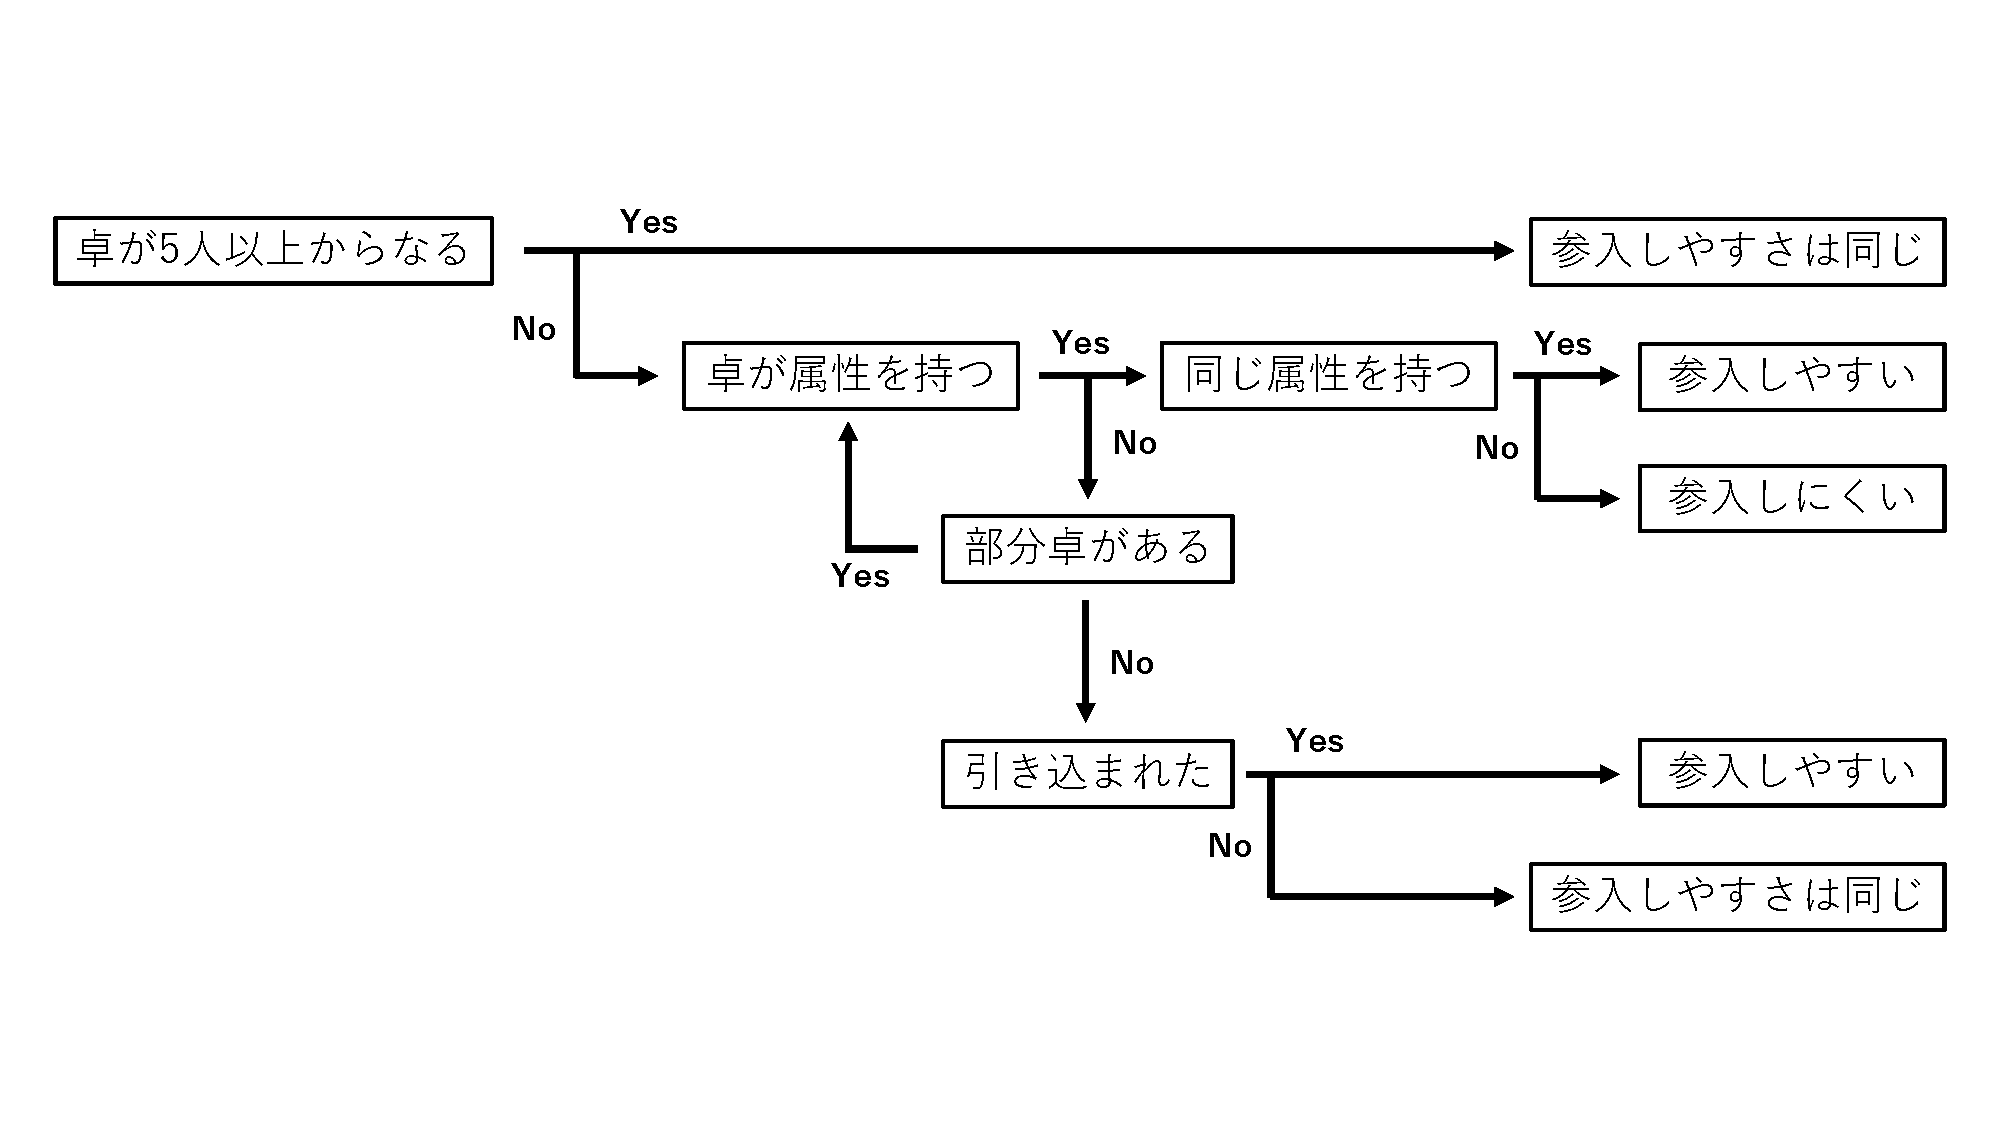
\includegraphics[height=6cm,width=12cm]{2025shinki/konpa_furumai/figures/takunokakudai_flowchart.pdf}
  \caption{拡大のフローチャート}
  \label{fig:kakudai.flowchart}
\end{figure*}
\par
前章で挙げた例では、次のように会話が進む。
\par
\dotfill
\par
\talker{鈴木}
自己紹介お疲れさま。

\talker{佐藤}
ありがとうございます。すごいですよね、めいも-------ん\footnote{SC新歓の自己紹介では、出身高校(または前の所属大学、予備校など)を言った後に参加者が「めいもーん」というコールをあげるという風習があった。自身の出自を明かすことを強制されるという側面に対する問題意識から、ここ数年でなくなってしまったが、筆者が入寮した時にはまだ残っていた。確かにノリについていける人とそうでない人で温度差はあったが、ああいった粗雑さの中に学生寮らしさを感じ取ったものだった。}って。出身校を名門だなんて言われたの初めてです。

\talker{鈴木}
ね。すごいよね。

高橋が加わる。佐藤の隣に座る。\textgt{〈卓の拡大\footnote{高橋が参入できたのは、恐らく高橋の立場やコミュ力の高さが原因だろう。}〉}
\par
\talker{高橋}
どーもー。

\talker{鈴木}
お疲れ様です。

\talker{高橋}
(佐藤に向かって)新入寮生の方ですか?

\talker{佐藤}
D101に住んでます、文学部1回生の佐藤です。

\talker{高橋}
佐藤さん。どうもD34に住んでる文学部3回の高橋です。

\talker{佐藤}
よろしくお願いします。

\talker{高橋}
寮で「佐藤さん」って意外と珍しいよね。

\talker{鈴木}
ですよね。

\talker{佐藤}
そうなんですか?

\talker{高橋}
そう。珍しい苗字は時々見かけるけど、この寮意外とメジャーな苗字がいなかったりするんだよね\footnote{これはその通りで、熊野寮ではメジャーな苗字は意外と見かけなかったりする。そこまで多くない苗字が意外と寮内ではメジャーな苗字だったりもする。}。

\talker{佐藤}
へぇ~。

田中がそばを通る。
\par
\talker{鈴木}
あ、田中だ。おーい。
\par
田中が加わる。鈴木と高橋の間に座る。\textgt{〈引き込みによる卓の拡大\footnote{田中が鈴木の隣に座ったのは、鈴木に引き込まれたからである。}〉}
\par
\talker{田中}
こんにちは~。

\talker{鈴木}
この子同部屋の1回生の子。

\talker{田中}
お~。(拍手)

\talker{佐藤}
D101の佐藤です。

\talker{田中}
田中と言いますぅ。

\talker{佐藤}
田中さんの学部はどちらですか?

\talker{田中}
理学部だよー。

\talker{佐藤}
理学部。へ~。

\talker{田中}
今年系登録できるか微妙だからやばい(笑)(ピース)

\talker{鈴木、高橋}
(笑い)

伊藤が加わる。佐藤と高橋の間に座る。\textgt{〈卓の拡大\footnote{なぜ鈴木の隣に座らなかったのか疑問に思った読者もいるかもしれない。しかし、もし伊藤が元寮長だとすれば、あるいは伊藤が新歓の場では積極的に1回生に話しかけに行くタイプであったとすればどうだろう。}〉}
\par
伊藤が加わった後の位置関係は図\ref{fig:example.2}のようになっている。ただし、三角形の向く方向はその人の身体や顔の向きを表している。
\begin{figure*}[htbp]
\begin{minipage}[b]{0.45\linewidth}
   \centering
  
\includegraphics[height=4cm,width=4cm]{2025shinki/konpa_furumai/figures/taku.example_2.png}
  \caption{伊藤が加わった後の卓}
  \label{fig:example.2}
\end{minipage}
\begin{minipage}[b]{0.45\linewidth}
  \centering
  
\includegraphics[height=4cm,width=4cm]{2025shinki/konpa_furumai/figures/taku.example_3.png}
  \caption{渡辺が加わった後の卓}
  \label{fig:example.3}
\end{minipage}
\end{figure*}
\par
\talker{伊藤}
お邪魔しま~す。

\talker{鈴木}
伊藤さん。うちのブロックの1回生の子です。

\talker{佐藤}
D101の佐藤です。

\talker{伊藤}
どうも工学研究科M2の伊藤です。来年退寮する老人です。学部はどこ?

\talker{佐藤}
文学部です。

\talker{伊藤}
へぇ~。どの分野やりたいとかあるの?

\talker{佐藤}
近世哲学とか興味あります。

\talker{伊藤}
カントとかヘーゲルとかのあたり?

\talker{佐藤}
あー、そうですそうです!

\talker{伊藤}
へ~。そこらへんは倫理で習っただけであんまり知らないけど面白そうだよね。熊野寮って哲学好きな人結構多いし。楽しめるんじゃない?

\talker{佐藤}
やっぱりそういう人多いんですか?

\talker{伊藤}
ごりっごりの哲学という感じではないけどそっち方面の話題が好きな人はやっぱり多いね。前に出てくる人とかごりごり寮自治してるよ、っていう人とかにそういう人が多いだけかもしれないけど。会議とか出てると「寮自治は何のためにやるのか」とか「寮祭はなぜやるのか」とかそういう話になることがしょっちゅうあるねー。

\talker{佐藤}
へー。面白そう。

\talker{伊藤}
お〜。これを面白いと思える人は結構寮生活向いてるよ。新歓とかたくさん行くと知り合いもたくさんできるし授業始まってからもすっごい楽しくなるから、自分の部屋とかにこもらずにどんどん談話室とか食堂とかに顔出すといいよ\footnote{文学部で、哲学好きで、なんとなく態度が前のめり。この卓の人間は皆、\textgt{佐藤}はこれから寮自治の中心に関わっていくに違いないと考えているだろう。ただ、登場人物たちは\textgt{佐藤}が好奇心旺盛であるという点を知らない。好奇心だけで動く人間は寮自治ではなく自治寮に興味があることが多い。自治活動に関わるきっかけの一つとして好奇心は重要だが、上回生になれば寮を維持・発展させるという責任感を持つことも求められる。}。
\par
\dotfill

\noindent{\uuline{\large\textbf{3.3.卓の分裂}}}\\
卓は人数が多くなると、違う話題を話す2つの卓に分かれることがある。これを「卓の分裂」と呼ぶことにする。分裂してできたひとつひとつのグループは、その内部で同一のグループに属しているという共通認識を持つことが多いので、それぞれが卓の条件を満たしている。
\par
分裂の仕方を一言で表現すると、同じ卓の中で違う会話の流れが生まれるということである。卓の振舞いで転機となるのは、複数人が同時に話始めることや、自分が話さない時間が長くなったりすることだ。複数人が同時に話し始めると、同じ卓の中で違う話を聞き始める人が生まれる。それぞれの話から再び会話が始まるので、違う会話をする2つのグループが生じ、それぞれ卓として振る舞うようになる。また、自分が話さない時間が長くなると、手持ち無沙汰になって隣の人と世間話をする人が出てくる。これによって複数人が同時に話始める状態が生まれ、上と同様にして卓が分裂する。さらに進むと、人の配置が変化して2つの輪ができる。そこまでくれば分裂したことは外から見ても明らかである。
\par
分裂のしやすさは、拡大といった他の要因を考えなければ卓の構成人数が多くなるほどしやすくなる。なぜなら、人数が多くなればその分自分が話さない時間が長くなったり、同時に複数人が話始めるタイミングが多くなるからだ。
\par
これまで述べた例でも卓の分裂を見てみる。
\par
\dotfill
\par
先ほど述べた例の最後の方では伊藤と佐藤の会話がメインであった。伊藤の話す時間が長くなったので、ここから卓が分裂していく。現在各登場人物の状況は以下のとおりである。
\begin{itembox}[l]{各登場人物の状況}
  \talker{佐藤}
  伊藤と話している。
  
  \talker{鈴木}
  佐藤がいい感じに会話に溶け込めてきたので、あとは気さくな伊藤に任せて他の参加者とも話そうかと思っている。
  
  \talker{高橋}
  できれば新入寮生と話したいので\textgt{佐藤}と\textgt{伊藤}の会話に参加しようと思っている。
  
  \talker{田中}
  手持ち無沙汰になっている。
  
  \talker{伊藤}
  佐藤と話している。
\end{itembox}
田中が鈴木に話しかけるところから卓の分裂が始まる。

\talker{田中}
鈴木は春休み何してたー?\textgt{〈卓の分裂〉}

\talker{鈴木}
何もしてない。談話室でごろごろしてたら2か月過ぎてた\footnote{あるある。談話室にいると何故か時間が溶けていく。}。

\talker{田中、鈴木}
(笑い)

\talker{鈴木}
田中は?

\talker{田中}
さすがにそろそろ頑張らないとやばいと思って、1回生の復習とかやろうとしてたら、なんか春休み終わってた~。

同時並行で進んでいる伊藤と佐藤の会話も見てみよう。
\par
(前項の会話の続きから)
\par
\talker{佐藤}
へ~。寮の新歓結構多いですよね。明日はD34?新歓がありますし。

\talker{高橋}
そう!明日D34新歓やるから来てね。

\talker{佐藤}
あ!確かに高橋さん?はD34ブロックでしたね。

\talker{伊藤}
めっちゃ食い気味(笑)。こっからブロック新歓って言って、各ブロックが主催する新歓が始まるんだけど、その1発目がD34の主催するD34新歓。ブロック新歓はブロックごとに特色があって面白いよ\footnote{筆者にとってブロック新歓巡りは春新歓の楽しみの一つである。新歓で提供される料理や、新歓内で行われるレクリエーションには、そのブロックの工夫やノリが垣間見えて面白い。1回生の時もブロック新歓は楽しみであったが、新歓を主催する側になると今度は料理の工夫やレクのアイデアを盗みたいと思うようになり、また楽しみが増えた。}。

\talker{佐藤}
へ~。楽しみです。
\par
\dotfill

\noindent{\uuline{\large\textbf{3.4.卓の安定性}}}\\
この章で述べた卓の拡大や分裂により、卓の安定性を考えることができる。まず、卓が安定しているとは、拡大も分裂もしにくい状態、すなわち卓の構成人数が変化しにくい状態のことであると定義する。本来卓の安定性には構成員の属性といった、様々な要因が影響していると考えられる。ただ、安定性の複雑な様相を論じることは本記事の趣旨から外れてしまうので、ここでは構成人数による安定性の変化について述べるにとどめる。
\par
まず拡大のしやすさに目を向ける。卓の構成人数が多くなりすぎると、物理的に参入できなくなるので卓は拡大しにくくなる。筆者の経験では、5人以上になると明確に拡大しにくくなる。これよりも人数が少ない場合を考えると、部分卓の属性が薄い場合や引き込みが起こらない場合は、人数が少ない方が参入する物理的なスペースが広く、参入しやすい。部分卓の属性がある場合は、人数が多くなるほど属性が希薄になり、拡大しやすさに及ぼす影響が小さくなる。引き込みも物理的なスペースの関係で、人数が多くなるほど起こりにくくなる。
\par
以上をまとめると、拡大しやすさは以下のようになる。
\begin{equation*}
  2人>3人>4人>5人>6人>7人>\cdots
\end{equation*}
\par
続いて分裂のしやすさに目を向ける。前節で述べたように、人数が多くなるほど分裂しやすくなる。ただ、2,3,4人の卓では、分裂しても卓にならない場合があるので、分裂しやすさは変わらない。また、6,7人以上の卓では、人数が多すぎて逆に分裂のしやすさは高止まりしてそこまで変わらない。まとめると以下のようになる。
\begin{equation*}
  2人=3人=4人<5人<6人\leq7人\leq\cdots
\end{equation*}
\par
以上2つをまとめると、卓の安定性は以下のようになる。
\begin{equation*}
  2人\leq3人\leq4人>5人>6人\geq7人\geq\cdots
\end{equation*}
これから分かるように、人数が極端に少ないときや極端に多いときは不安定になる、つまり構成人数が変化しやすいということが分かる。最も安定しているのは3,4人の卓である。
\par
卓が不安定な状態から安定な状態へと遷移する過程を例示する。
\par
\dotfill
\par
前項で挙げた例では、卓は\textgt{鈴木}―\textgt{田中}の卓と\textgt{高橋}―\textgt{伊藤}―\textgt{佐藤}の卓に分かれている。\textgt{鈴木}―\textgt{田中}の卓はいわば卓の赤ん坊のようなもので、不安定である。ここにもう一人加わると安定した卓になる。この例では1回生の\textgt{渡辺}が加わることで安定化する。
\par
\talker{渡辺}
入っていいですかー?

\talker{田中}
どうぞどうぞー。\textgt{〈卓の拡大〉}

\textgt{渡邉}が\textgt{田中}と\textgt{鈴木}の間に座る。このとき卓は図\ref{fig:example.3}のようになっている。各登場人物の体の向きを見てみれば、卓が2つに分かれている様子が分かると思う。

\talker{鈴木}
1回生?

\talker{渡辺}
あっ、はい。農学部1回生の渡辺です。

\talker{田中}
自己紹介の時に寮の声明文とか読んだことあるって言ってた人\footnote{SC新歓で印象に残る自己紹介をすると覚えてもらえやすい。ただ、みんなそのうち覚えてくれるし、自己紹介は上回生側が大いに盛り上げるものなので、面白いことを言おうなどと変に気負わず適当に切りぬければよい。}?

\talker{渡辺}
あ!はい、そうなんです。

\talker{鈴木}
え、声明文読んできてるの?

\talker{渡辺}
はい。寮祭の企画で呼び出されたっていうニュースを見て、どうやら寮が声明文を出していたらしいということで実際に調べてみて読んで、

\talker{田中}
おー。めっちゃ有望(笑)

\talker{鈴木、渡辺}
(笑い)

\talker{田中}
高校生の頃に読んでどんな感想抱いた~?

\talker{渡辺}
意外とちゃんとした理由があったんだー、という感じですね。あとは大学に文句を言って停学になったって知ってびっくりして。要求項目に書いてあることとか、例えば職員の正規雇用化とか、確かにそうだな、と思うものも結構あったんですけど\footnote{ここで話されているのは、2022年の寮祭で行われた総長室突入という企画について、それに参加した学生のうち5人が処分された、という実際の出来事についてである。寮のHPには突入時の声明文、処分に対する声明文等、総長室突入に関する声明文は豊富にあるため、一度そうした文書に目を通してみてほしい。}、

\talker{田中}
ね~。大学がおかしいって言ってるのに処分されるのほーんとに意味わかんないよね。

この後は、しばらく両方の卓で会話が進む。最終的にどうなるかということについては、次章で述べる。
\par
\dotfill

\noindent{\uuline{\Large\textbf{4.卓の散逸、消滅}}}\\
言うまでもないが、出来上がった卓はいつまでもそこにあるわけではない。長く維持されたとしても、最終的にはコンパの終了とともに必ずなくなる。そこで、本章では卓がなくなる様子について説明する。
\par
まず、卓がなくなるとはどのような状態を指すのかについて、本記事内での定義を与える。卓が生成されたのち、拡大や構成員の入れ替えをしながら、しばらくその卓は維持される。3章で述べたのはそうした連続的な卓の変化であるから、できてすぐの卓から連続的な変化を遂げた卓は、どの状態にあっても同じ卓とみなすべきである\footnote{分裂した後の卓まで同じ卓とみなすかどうかは判断に困るところである。はじめの円形の形を保っていれば同じ卓とみなしたいが、物理的に2つに分かれてしまえば、それはもともとあった卓とは違う卓とみなした方が自然である。ただ、本記事では卓の分裂をどう捉えるかはさほど本筋とは関係ないので、考慮しないことにする。}。それゆえ、卓がなくなるとは、卓の連続的な変化が打ち切りになること、と定義づけられる。これには以下に述べる「卓の消滅」と「卓の散逸」の2種類がある。

\noindent{\uuline{\large\textbf{4.1.卓の散逸}}}\\
コンパでの卓の無くなり方として、次のような場合があり得る。4人で談笑している卓で、日付を越えたあたりで一人が帰り、その後しばらく話したのちに別の一人が眠くなったので帰り、残った2人も夜が更けてきたので解散する、といった場合である。これも卓がバラバラになって最終的に消えているので、卓がなくなる一例だと言える。このようなケースは、コンパ終盤の夜中の1時、2時頃によくみられる。このように卓がなくなることを、構成員が少しずつバラバラになっていく様子を表現して卓の散逸と呼ぶことにする。明示的に述べれば、卓の散逸とは、卓の構成員が少しずつ卓から離れていくことで、徐々に規模が縮小し、最終的に消えてしまうこと、ということになる。上に挙げた例のように一人ずつ離れるのではなく4人一斉に解散することも、ここでは卓の散逸と捉えることにする。
\par
\dotfill
\par
前章での会話からさらに時間が進み、12時を過ぎた。始まったときにはあれほどにぎやかだった食堂も人が少なくなり、今は卓が2,3個あるのみである。寂しくなったので誰かが寮祭動画を流し始める\footnote{コンパあるある。日付をまたいで人が少なくなってくると、誰かが食堂に常設されているモニターで寮祭動画を流し始める。}。
\par
(\textgt{鈴木}―\textgt{田中}―\textgt{渡辺}の卓では)
\par
\talker{田中}
お、寮祭動画だ。寮祭は毎年あんな感じで動画を作って記録するというのをやっていて、あれ去年のやつだね~。

\talker{渡辺}
おー。(拍手)

\talker{田中}
いつもの恒例企画もありつつー、毎年突然変異みたいに出てくるいろんな意味でのカミ企画も残っていたりするから意外と面白い。

\talker{渡辺}
あっ、時計台コンパだ\footnote{恒例企画の1つ。時計台の前で畳を敷いて料理を振る舞ったりライブをしたりして、キャンパス内で寮祭の開幕を祝う。京大らしさを感じることのできる企画だ。読者も入寮したら憧れる側から作る側に回る。寮祭では、こうした恒例企画をただ傍から楽しむだけでなく、一緒に運営することが求められるのである。}!

\talker{鈴木}
さすが。よく知ってるね。

寮祭動画が終わる。\textgt{高橋}―\textgt{伊藤}―\textgt{佐藤}の卓がどうなっているかを見てみよう。

\talker{高橋}
おー。(拍手)

\talker{佐藤}
さすがに日付を越したのでそろそろ寝ます\footnote{\textgt{佐藤}は動画が終わったから帰る、という体で帰ろうとしているが、恐らく寮祭動画が流れる少し前から卓から抜ける機会をうかがっていたのだろう。寝たいけど会話が弾んでいるからタイミングをつかめない、という状況は筆者にとってもいまだにある。どちらも悪くないのでこればかりはしょうがないと思っている。}。

\talker{高橋}
さすが1回生\footnote{本当に初々しい。入寮したてはこんなことを言っていた\textgt{佐藤}も、1か月経てばすっかり寮生になって深夜2,3時までは平気で起きているようになるのだろう。って\textgt{高橋}は思っているはず。}。おやすみなさい。

\talker{佐藤}
おやすみなさい。\textgt{〈卓の散逸〉}

\talker{伊藤}
そうか。1回生にとってこの時間は深夜なのか。

\talker{高橋}
そういえばそうですよね。なんか初々しい。

\talker{伊藤}
ねー。

(話題がなくなって一瞬静かになる。)

\talker{伊藤}
もう少し居たいけど明日も予定があるので寝ようかな。

\talker{高橋}
伊藤さんにしては珍しいですね。

\talker{伊藤}
確かにねー。いつも名残惜しくてずるずると夜更かししちゃうけど。院生になってから昼間に研究の予定が入るようになってなかなか夜更かしできなくなっちゃった。

\talker{高橋}
健康生活。

\talker{伊藤}
そう。院生になってから研究が思いのほか仕事だったから早寝早起きじゃないとやってられなくなって、逆に健康になってる。

\talker{高橋}
おー。(拍手)

\talker{伊藤}
このまま話し込んでたらまた寝れなくなっちゃうから撤退します。おやすみなさーい。

\talker{高橋}
おやすみなさい。\textgt{〈卓の散逸〉}

畳は明日の昼間に片づけようということになったので、\textgt{高橋}も寝ることにする。これで\textgt{高橋}―\textgt{伊藤}―\textgt{佐藤}の卓が散逸しきった。
\par
\dotfill

\noindent{\uuline{\large\textbf{4.2.卓の消滅}}}\\
他にも、卓を構成している人たちがまとまってどこか別の場所に行くことがある。そうして会場から卓が丸ごと無くなることを、卓の消滅と呼ぶ。例えば、4人で談笑している状態で、誰かが外に雪が降っているから見に行こう、と言い出したとする。このとき他の3人が賛成すれば、4人はコンパの席を外し、外に出ることになる。するとこの卓はこれ以上コンパの場で変化することはないので、卓はなくなると言える。このようなケースでは、4人が一斉に席を外す様はまるでコンパの場からいきなり卓が丸ごと無くなるように見える。\footnote{上のような消滅の仕方は、一般にはあまり良くないこととされている。理由は様々だが、コンパ主催者と参加者の間でサービスの授受をする構造が見え隠れしていることが主なものだろう。コンパはあくまで寮生間の広い交流を促進するためのもので、みんなで準備してみんなで楽しんでみんなで片づけるというのが原則なのだ。}。この例の他にも、4人でボードゲームをしに談話室へ行くケースや、コンパと同時開催されている別のイベントに参加しに行くケースなどがあり得る。
\par
卓の消滅との大きな違いは、卓の構成員がまとまって移動するか否かにある。消滅する場合は構成員(あるいはその中の数人)がまとまって別の場所に移動するが、散逸では構成員はバラバラになって別の場所に行く。消滅と比べると散逸は自然な無くなり方である。
\par
\dotfill
\par
最後に\textgt{鈴木}―\textgt{田中}―\textgt{渡辺}の卓を消滅させる。
\par
(寮祭動画が終わる。周囲でファミリーマートに行く機運が高まる。)
\par
\talker{田中}
追加買い出しの機運かな~。

\talker{鈴木}
行く?

\talker{田中}
行く行く~。

\talker{渡辺}
追加買い出しって何ですか?

\talker{田中}
お酒とかがなくなってきたのでファミマに買いに行くんだけど~、新入寮生は好きなお菓子とか買ってもらえるからついていくのがおすすめ。

\talker{渡辺}
へ~。それなら行ってみます。

\talker{田中}
よしっ!(ガッツポーズ)\textgt{〈卓の消滅〉}

追加買い出しから帰ってきたら再び\textgt{鈴木}―\textgt{田中}―\textgt{渡辺}の卓ができると思われるが、食堂にいる人から見れば一時的に卓がなくなったように見えるので、卓の消滅の例として挙げた。このような消滅の仕方は健全である。
\par
\dotfill

\noindent{\uuline{\Large\textbf{5.おわりに}}}\\
本記事では、コンパの場で見られる「卓」と呼ばれるグループについて、その振舞いを論じた。最初にどの程度の性質をもったグループを卓とみなすのかを明示的に定め、卓が完成する様子を描写した。その後に3章で出来上がった卓が経る変化として卓の拡大と分裂について紹介し、4章で卓が最終的に迎える末路として卓の散逸と消滅について述べた。本記事で卓の振舞いを一通り言語化したことで、筆者と似たような興味を抱く方々に、今後卓を考察していくうえで一つの骨格となるものを提示できたように思う。
\par
本記事の大きな成果として、卓の安定性について述べたことが挙げられる。卓には安定しているものと不安定なものがあり、それは構成人数や構成員の関係性などが複雑に混ざり合って決定している。構成人数が与える影響については本記事で述べたとおりだが、構成員相互の関係性、個人のバックグラウンドが与える影響まで考慮できれば、安定性の理論を日常の場に応用していくことができるようになるだろう。例えば春入選\footnote{入寮選考の略。実際は合否を決めることはないので、新入寮生が入ってくるというイベントのことを指すことのが一般的。受け入れブロックを決める際には、(特に1回生の場合)趣味などで疎外感を感じたりしないか、自分のブロックの雰囲気に馴染めるか、といったことが考慮される。また、これからのブロック自治を担う存在であるため、仕事をしてくれそうか、寮自治への理解はあるか、といったような政治的な側面も考慮される。}で各ブロックが1回生をどのように迎え入れれば仲良くなれるのか、談話室の中で疎外感を抱く人がいないようにするにはどのような座り方で座ればよいのか、といったことが演繹的に理解できるようになる。安定性理論については、安定性に影響を与える要因を明らかにすることに加え、予測を可能にする数理モデルの構築も課題だ。
\par
また、コンパにおける卓の振舞いの理論は、会話の中にはたらく力学を考察する上で抽象度の高い理論である。なぜならば、コンパの卓には物理的形状や構成人数に制限がなく、自由度が高いからだ。本記事では一般論としてコンパの卓について述べたが、はじめに言及したように卓はコンパの場に限らず日常的にみられるものである。例えば寮食の喫食時間中にできる卓であれば、物理的形状は食堂の椅子の配置によって規定されており、また構成人数も高々6人程度で、4人までが標準的である。このような卓は制約が多い反面、それだけ具体的で考察しやすい。対象を具体化して考察方法を確立し、理論の土台を作ることは今後必ず手を付けねばならない課題だ。
\par
  コンパはたくさんの人がいて、入寮してしばらくしても知らない人と邂逅したり、いつも話している人の新たな一面を知ったりと、新鮮な出会いが絶えない楽しい場である。ただ一方で人と話す気分でないときや疲れているときは、やや居心地が悪い場所でもある。しかしコンパの楽しみ方は人と話すことだけではない。人と話せないがコンパの場には居たい、という日には、ぜひ卓がどのように変化するのか、卓の中で人々の意識の流れがどのようになっているのか、ということを考えてみてはいかがだろうか。
\end{multicols}


  \newpage
  \section{ 熊野寮的ヤマノススメ}


京都は盆地である。われわれが夏は暑く冬は寒い、お世辞にも過ごしやすいとは言えない環境に置かれているのもこの地形のためという。しかし疎ましい雨が地を潤し実りをもたらしているように、この世の大抵のものはデメリットばかりではなく、見方を変えてみればメリットもあるものだ。盆地とはすなわち平地が山に囲まれた地形であり、「山が近い」ということは山を登る人にとってはメリットとなる。自転車やバスで気軽に行ける範囲に、半日で登れる風光明媚で古くから信仰の対象ともなってきた山がいくつもあるのは京都ならではのことだ。どうせ京都に住むのなら、山を疎むのではなく楽しんでしまおうというのが、この記事の趣旨である。以下では初心者向けのおすすめの山について、寮からのアクセスと筆者のお気に入りポイントを解説する。なお、筆者は登山部でもなんでもなく年に数回ハイキングするだけの素人であるので、専門的な知識はないがあしからず。そして注意点として、どんな低い山にも事故のリスクはあるということを心に留めておいてほしい。体調の悪い時は登らない、動きやすい服装をする(長袖長ズボンがのぞましい)、十分な水と食料を持ち込む、日のあるうちに余裕を持って下山できるスケジュールを組むなど、誰にでもできる対策で構わないので安全には配慮していただきたい。

\subsection{①大文字山 標高:472m}
五山の送り火で大の字が点火されることで知られる。テレビで一度は見たことがあると思う。火床に足を踏み入れられるのと、思い立ったらすぐ登れるくらい簡単なのが良いところ。
寮からは自転車で10分ほどで、登山口はいくつかあるがどのルートでも登りやすいことに変わりはないので好きに選ぼう。自転車の場合は、ふもとの怒られなさそうなところに停めておこう。車の邪魔にならないかつ私有地ではない場所を選べばそうそうしょっぴかれないはずである。大勢で登りたければ、毎年文化部が開催する大文字コンパに参加しよう。
\subsection{②比叡山 標高:848m}
天台宗・最澄とセットで覚えさせられた、あの山である。滋賀県との県境に位置し、じつは山頂は滋賀県側なので延暦寺は京都のものではない。山登りのついでで延暦寺に参拝したり、琵琶湖を見下ろしたりできる一石三鳥な山。
寮からは自転車を使ってもいいが、登山口付近は住宅街でコインパーキングも停められそうな空き地もなく、叡山電鉄修学院駅横の駐輪場に停めることになるので、自転車で行っても結局駐輪代がかかるし登山口まで近いわけでもない。このため、出町柳駅から叡山電鉄に乗ることを推奨する。登山ルートは有名なきらら坂ルート(修学院駅)か、雲母坂ルートよりやや短い梅谷ルート(三宅八幡駅)の2つがおすすめ。それなりに登りがいのある山だが、大学生なら登山靴や杖がなくても普通の運動着で登り切れるくらいの手頃さである。ちなみにケーブルカーやドライブウェイが整備されているので、ハイキングをしなくても山頂に到達することができる。登っていて疲れ切ってしまったときは下りだけこれらに頼るのもアリ。
\subsection{③愛宕山(あたごやま) 標高:924m}
嵐山界隈に位置する、関西では火防の神として有名な愛宕神社がまします山。筆者のバイト先のキッチンにもここの御札が貼ってある。市街地からそこそこ離れていて、登山口ですら清らかな川を見ることができる。山頂の神社には手水舎がないので、参拝前に手を清めたい人はここの川の水を汲んでおこう。表参道はかなり広めの道幅が確保されていて、複数人で横に並んでも歩きやすい。丹波山地の南端に位置するため、北を見れば山海が広がり、南を見れば京都の市街地が見下ろせるのもおもしろい。
寮からはバスで一時間ほど揺られて向かう。熊野神社前や京都市役所前から嵐山方面のバスはそれなりに本数が出ているが、登山口である清滝停留所まで出る便は少ないので要チェック。標高は比叡山とそこまで変わらないが、筆者の主観的には比叡山よりも1.5倍ほどハードだった。登った時期の問題かもしれないが、高低による気温差が他の山よりも激しいように感じた。しかし厳しい分登ったときの達成感もひとしおであり、山頂の鳥居を見たときの喜びは忘れられない。実は細くはあるが山頂付近まで伸びる車道があり、ツーリングで来る人もいるらしい。バイク乗りの方は検討してみはいかがか。

文責:タケッシ

  \newpage
  


\section{女子寮生向けハラスメント相談窓口より}

%文責扱いで
\author{女子寮生向けハラスメント相談窓口} 

\subsection{はじめに}
こんにちは、女子寮生向けハラスメント相談窓口です。私たちは、熊野寮に住む女子寮生によって組織されていて、女子寮生が暮らしやすくなるように様々な活動を行っています。私たちのアプローチの対象は寮内の女性だけでなく、寮外の「熊野寮に入寮するかもしれない人たち」も包含しています。以下の文章は、私たちが、熊野寮生の出身校に送付することを目指して作成した冊子を加筆・修正したものです。

%タイトルみたいな形にしたい
\noindent{京都大学熊野寮女子寮生から高校生のあなたへ}

\vspace{3cm}

\begin{figure}[hbp]
\centering
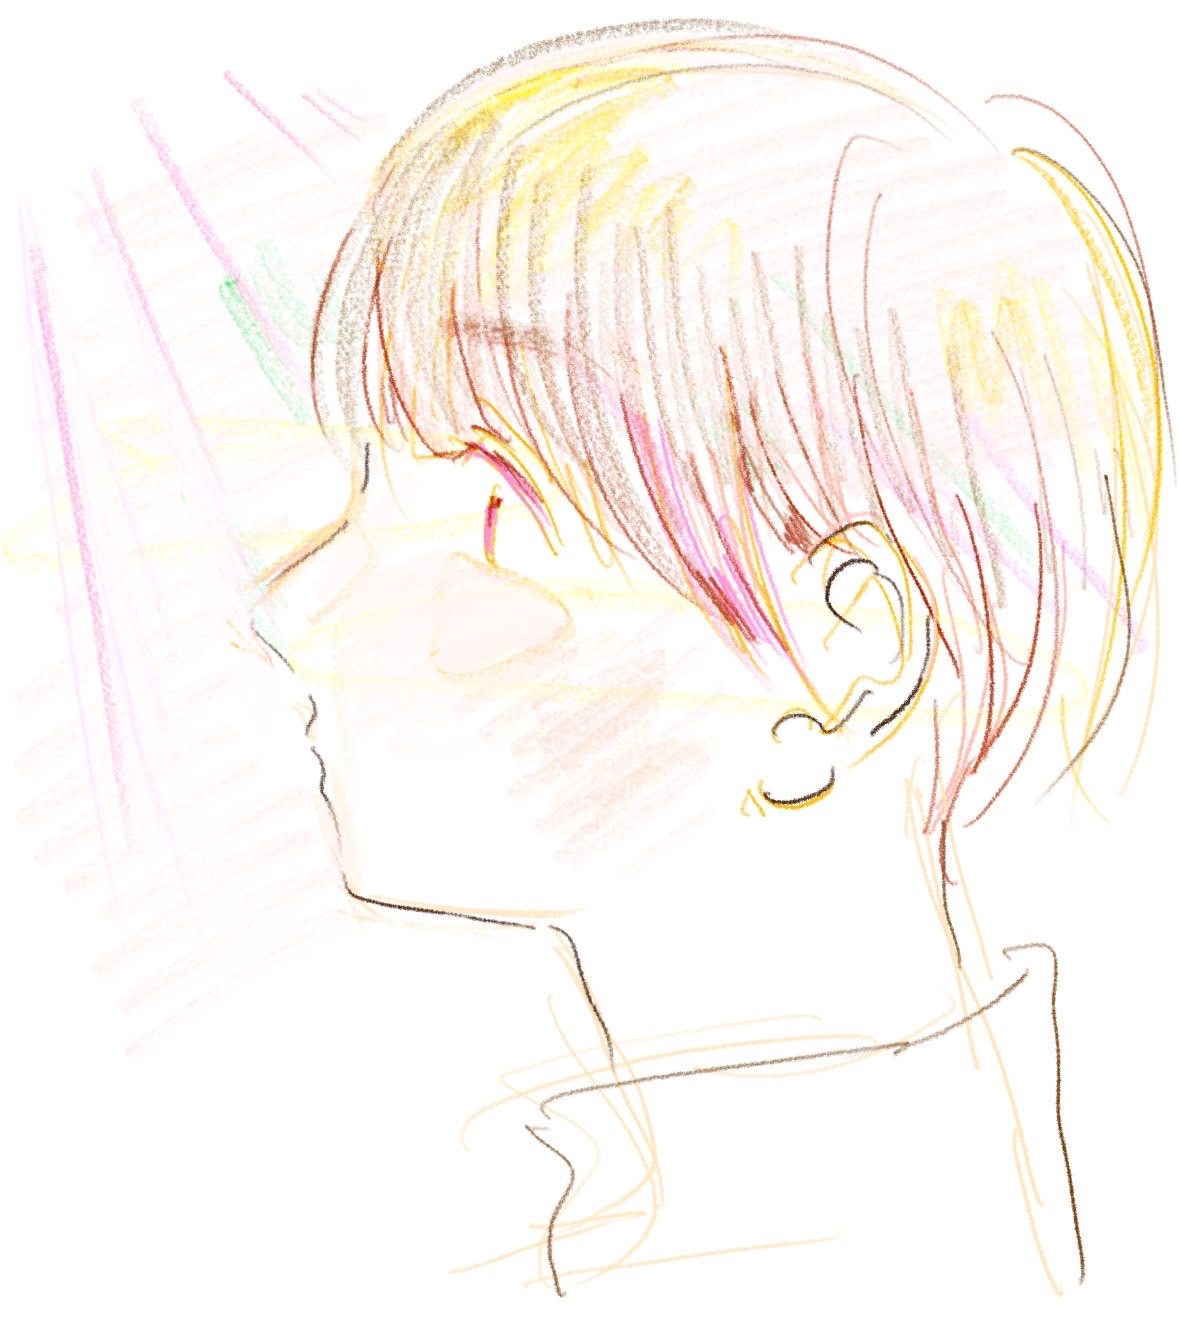
\includegraphics[width=8cm]{2025shinki/joshi_ryosei/kijigazo.jpg}
\end{figure}




\subsection{まえがきのようなもの}
\hfill {文責:翠}

\begin{flushleft}
あなたへ
\end{flushleft}
\vskip\baselineskip
まずは、この冊子を手に取ってくれたあなたに大きな感謝を。

この冊子は、京都大学の学生寮である熊野寮における女子寮生向けハラスメント相談窓口(以下、女子寮生窓口)という団体が主体となり、実際に寮に住む女子寮生の寄稿によって出来上がったものです。日本の高等教育では女子の比率は男子に比べて少なく、京都大学や私たちの住む熊野寮においても例外ではありません。熊野寮内において、女子寮生の数は全体の2割程度です。「女子 (ここで述べる女子(女性)とは、生物学的に女性の身体をもち、女子トイレや女子シャワー室を利用する人たちを指します)」という属性を持つ私たちはマイノリティであることを一つの理由として日々もやもやとした思いを感じることがあります。私たち女子寮生窓口のメンバーは、女子寮生が感じるそういった生きづらさ、住みづらさを解消するため、日頃は匿名での相談受付や女子寮生新歓の開催を行っています。そして、これから先の進路に迷ったり迷わなかったりしている高校生のあなたに、女性という属性を持つ人生の少し先輩として、今の生きづらさやこれから直面するであろう生きづらさに対処していくためのヒントが渡せたらいいなという思いから、この冊子を作り、届けることになりました。(もちろん、高校生でない方にも、京都大学の一学生が考えていることをふむふむと読んで楽しんでいただければと思っています。)
\vskip\baselineskip
現状、悲しいことですが、性差に基づく生きづらさが社会の中に存在しています。

女性を例に挙げると、女が勉強なんてとんでもないという価値観に縛られて大学や大学院に行きにくかったり、実家を離れて生活することに難色を示されたり、男女の夫婦関係において家事育児の負担を多く担っていてキャリアを犠牲にしたり、化粧やスカートの着用を強制されたり、満員電車や夜道に性被害の恐怖が伴ったり…。

でも、これは、女性だけの生きづらさではなく、男性と女性のどちらにも当てはまらない性の在り方をもっている人や男性においても、それぞれの人にとって形を変えて眼前に現れるものであると思います。女性の生きづらさの根源は、生物学的性に基づく、男らしさ女らしさの強制であり、多様な性的な在り方の否定です。あらゆる属性の人間1人1人がもつ大きな可能性を握りつぶす抑圧です。そういうのが、社会にはずーっと前から今まであり続けて、男性や女性やすべての人を息苦しくさせているのです。

私たち女子寮生窓口は形式上「女子」寮生向けとなって女性に焦点を当てているけれど、最終的には、男性もその他の性を持つ人も、むしろすべての人が性別に起因する生きづらさから解放されることを目指しているのじゃないかと思っています。少なくとも、私はそうあってほしいと思いながら活動をしています。20何年生きてきた私自身、自分が女であるということを否定できない事実として受け止めている一方で、今でも自分が性的にも社会的にも女であることを強く否定したい気持ちに襲われます。そういう男とか、女とか、関係ない社会になればいいのにね、という話です。

すこし大きな話をしてしまいましたが、これから先に掲載されている文章は熊野寮女子寮生や元寮生の日常的でささいな思いの表出です。こんな女性が京都大学にいて生活しているのだというロールモデルを提供できたらそれはとても嬉しいですし、あなた自身の人生において、やりたいことをやる後押しができたのなら、それはもっと嬉しいです。
\vskip\baselineskip
\begin{raggedleft}
かつてあなたと同じ境遇だったかもしれない私より
\end{raggedleft}
\newpage

\subsection{一人暮らしから熊野寮へ}
\begin{flushright}
総合人間学部 5 回生 H.O.
(2024 年春入寮)
\end{flushright}

\subsubsection{はじめに}
この文章は、この春、熊野寮に入った一人の女子寮生である私の生活について綴ったものです。「女性であること」についての言及はそこまで多くありませんが、この文章を読んで少しでも皆さんが「熊野寮に暮らす女性」をより鮮明にイメージでき、身近に感じるようになればいいなと思い、寄稿させていただきました。
\vskip\baselineskip
私が熊野寮に引っ越してきたのは、大学“5 回生”になる春休み、3 月末のことだった。もうすぐ4 月だというのに、冷たい風が吹き荒れて雪の舞う、寒さの厳しい夜。4 人部屋のルームメイトの 1人から手渡された合鍵を大事に握りしめて、これからの寮生活に胸を高鳴らせた。

\subsubsection{私が熊野寮に入るまで}
 私が京都大学に入学したのは 2020 年 4 月、新型コロナウイルス流行に伴う外出規制がちょうど始まった頃だった。大学の授業は全てオンラインだったので、1 回生の前期は福井の実家で過ごし、後期から京都に移り住んで、元田中駅近くの 1K のアパートで一人暮らしを始めた。それ以来、4 回生の終わりまで合計で約 3 年間(3 回生で半年留学をした期間は除く) 、私はそこで暮らした。白い床と白い壁の部屋に合うよう、家具は淡い木目調で揃えた。決して広くはないがかわいらしいその部屋を、私は気に入っていたはずだった。それなのにいつの間にか、私は部屋にいても落ち着かなく感じるようになってしまった。 「自分は一人暮らしよりも、誰かと一緒に住む方が幸せだろうな」 。ひとりで作った夕食を、iPad を相棒にして食べるとき、そんな考えが止められなくなったからだ。
\vskip\baselineskip
 留学の関係で 1 年留年して“5 回生”となった私は(大学に来てから知ったことだが、様々な理由で 4 年よりも長い時間をかけて学部を卒業する人というのはけっこういる)、大学生活最後の 1 年を過ごす場所として熊野寮を選んだ。1 回生の頃から「熊野寮祭」などのイベントに遊びに来て、寮が楽しい場所だと知っていたから、そこで多くの寮生と知り合いになったから…というだけなら、おそらく私は入寮には踏み切らなかった。かつての私にとって、熊野寮はあくまで「非日常」で「お祭り騒ぎ」の場所であり、自分がそのカオスの中で生活するイメージはまるでつかなかったからだ。転機となったのは、特別仲の良い友人が、昨年秋に寮に移り住んだこと。入寮後すぐ「友達はできたの?」と聞くと、満面の笑みで「大友達、大出来」と返ってきた。 「おおともだち……おおでき…。 」あまりに勢いの良い返事に呆気にとられながら、私は、今の自分が求めているのはこれなのではないかと思った。ひとりきりのご飯は虚しい。虚しさとは真逆のところに行ってみたい。人がいっぱいいて、それも皆個性的でバラバラで、いつもどこかで何かが起きていて、笑っちゃうくらい情報ぎゅうぎゅう詰めのところに。親友に寮の中を案内してもらい、それまで見たことのなかった炊事場や居室、シャワー室などの、寮生の居住エリアを一通り見せてもらった。壁の落書きやビラなど、たしかにゴチャゴチャしているけれど、これなら意外と普通に住めるかも、というのが感想だった。他のシェアハウスやドミトリーも検討していたが、 「熊野寮に住む」という選択肢が、一番わくわくした。当時の私の直感は間違っていなかったと、今振り返って思う。
\vskip\baselineskip

 2 月末の入寮面接を終え、無事、寮に住むことが決まったものの、引っ越しには苦戦した。3 年間の一人暮らしで溜め込んだ荷物を処理しきれないまま引っ越し当日を迎えた私は、初めて入る談話室\footnote[1]{同じ階(ブロック)の人が集まってくつろぐリビングのような部屋。ゲームをしたり映画を見たり漫画を読んだり課題をしたり、使い方は人によって様々である。}の引き戸を開けるなり真っ青な顔で「引っ越しを手伝ってくれませんか!?」と懇願する、迷惑な新入寮生と化した。 「あの…あと 1 時間で前のアパートの退去なんですけど、まだ…まだ中に荷物が残ってて…!」と、火事の建物に人が残されているかの如く切実に訴えた日のことが、昨日のように鮮明に思い出せる。幸い、その時談話室にいた同じ階の優しい住人たちのおかげで、私はなんとか熊野寮への引っ越しを完了したのだった。

\subsubsection{新歓と「居場所」の広がり}
 入寮してからの日々は、とんでもない速さで過ぎていった。春の間は怒涛のような新歓の連続で、新入寮生の私は、5 回生なのに行く先々で歓迎された。自分の 1 回生当時、コロナ禍で新歓がサークル活動ごとなくなってしまった分を余裕で取り戻すどころか、お釣りが来るくらいの歓迎されっぷりに驚いた。新歓といっても、アルコールを強要されたり嫌なノリを押し付けられたりすることはなく、ご飯やお菓子を囲んでおしゃべりする平和なものだ。各ブロックの新歓、部会や委員会の新歓、軽音にボードゲームなど趣味の集まりの新歓に加え、女性の寮生が集う「女子寮生新歓」というのもあった。ポトフやガパオライスなど、料理好きの寮生たちが腕を振るったとりどりの料理を一緒につつきながら、大学やバイトといった他愛もない話をして仲良くなった人たちとは、その後寮のシャワー室や食堂で顔を合わせたときにも言葉を交わす友人となった。こうしたコンパなどがきっかけで、寮の中に「ほっとする居場所」が作られていく感覚は幸せで、ありがたかった。

*

 あっという間に季節は過ぎて、12 月。入寮から 9 ヶ月が経とうとしている今、すっかり馴染んだ談話室のこたつで、私は筆を執っている。

\subsubsection{寮生として一度きりの「熊野寮祭」 、全てを詰め込んだ 10 日間}
 
先日まで、寮の最大のイベント「熊野寮祭」が行われていた。外から遊びに来るのではなく、寮の中の人間として参加する寮祭は、自分にとってこれが最初で最後。悔いのないよう楽しみ尽くそうと張り切った 10 日間は、それはもう盛りだくさんだった。ずっと出てみたかった名物企画「エクストリーム帰寮 \footnote[2]{夜中に車で知らない土地に降ろされた参加者が、地図・スマホ・現金を使わずに徒歩で熊野寮に帰ってくる企画。通称「エク帰」 。毎年 X(Twitter)等でも話題になる、熊野寮祭の名物企画。}」に友人とともに参加し、宇治から大津を経由して帰ってきたその足で、大量のスポンジケーキを並べて「ケーキコンパ\footnote[3]{スポンジケーキに好きなトッピングを載せて飾り付け、その独創性を競う企画。今年は「おいしい部門」 「美しい部門」 「ゲテモノ部門」の 3 部門で投票が行われた。}」を行った。ある夜は「方言マルチリンガル」になるという野望を掲げ、北は北海道弁・南は沖縄弁まで、全国津々浦々の方言話者と戯れた。またある夜は「福井県民コンパ」と称して、地元福井の名物を振る舞った。ある朝には早起きして、ホテルの朝食ビュッフェを自らの手で再現する企画のために、だし巻き卵を大量に巻いて…。寮祭について語ろうとすれば、紙面がいくらあっても足りない。ここまで挙げたのは、私自身が主体となって参加・運営した企画だけで、全体で 500 を超える寮祭企画のほんの一部にすぎないのだから。
\vskip\baselineskip

もう一つ、寮祭の中で忘れてはならない出来事が、音楽好きの寮生たちによる、3 日間にわたるライブだ。私は 3 日間で 3 つのバンドに出演し、うち 2 つでボーカル、1 つでドラムを担当した。私がドラムを務めるのは、なんと同じ部屋の人たちと一緒に組んだ“部屋バンド”。とある休日の朝、部屋で話していると「この部屋でバンドやりたくない?」という話になり、私は早速その日の午後に楽器屋に走ってドラムのスティックを買った。9 月初めのなんてことのない曇りの日が、部屋バンドの結成で急にきらきらと愛おしく輝きだしたのが懐かしい。1 年前の自分は想像しえただろうか?1 年後の自分が、同じ部屋の人とバンドを組み、ドラムを叩いてライブに出ているだなんて。不思議な世界線に生きているものだと、つくづく思う。
\vskip\baselineskip

 ライブや寮祭、コンパのような「ハレ」のまばゆいまでの楽しさと、毎日の寮食や談話室での会話のような「ケ」の中に散りばめられた喜び。それらを噛み締めて、1 日 1 日を大切に過ごしているつもりだけれど、きっと寮を出るまでの残りの日々も、忙しくてあっという間なのだろう。 「追いコン」で追い出される日も、きっとすぐだ。それまで、寮で出会った様々な人とのつながりを大切に、今、ここでしかできないことを追いかけるのだ。

\subsubsection{おわりに ―大学生活、どこに住もうか考えているあなたへ}
 一人暮らしには、一人暮らしの良さがある(入寮後、稀に、自分で自由に使えるきれいな個室が恋しくなる) 。人によって、共同生活が好きな人もいれば、一人暮らしの方が好きな人もいる。同じ共同生活でも、実家に家族と住むのか、シェアハウスに友達と住むのか、はたまた寮に住むのか、どんな寮なのか…選択肢はさまざまだ。この文章を読んで少しでも「熊野寮いいな、楽しそう!」とピンときた人は、きっと私のように、この寮を楽しむ素質のある人だ。そういう人にはもれなく、ぜひ一度寮に遊びに来てもらいたいと思う。

\vskip\baselineskip
 高校生の皆さんは、大学では一人暮らしを考えている人も多いだろう。まずは一人暮らしに挑戦してみる、という選択も一つだが、そのときに覚えておいてほしいのは、暮らし方は常に、ひとつではない、ということだ。今の暮らしとは別のところに、心躍る出会いが待っているかもしれない。もしも一人暮らしに飽きてしまったら、いつでも寮に来ればいい。熊野寮は、毎年春と秋の 2 回、入居者を募集している。この文章を読んでくれたみなさんの頭の隅に、 「熊野寮で暮らす」という選択肢が置かれるようになったなら、これ以上嬉しいことはない。

\newpage

\subsection{勇気をくれた仲間、大切な居場所}
\begin{flushright}
 文責:U.N. 
\end{flushright}

京大に入学してから、自身の「女性」という性別を意識する機会が増えた。意識するというより「させられる」という表現のほうが適切だろうか。大学そのものに加えて、私が自ら飛び込んだチャレンジングな環境は、往々にして女性が少なく男性が多い場所だった。その中でも、私にとって重要な居場所は2つある。第一に、進学と同時に入寮した熊野寮。第二に、進級を機に入部した、とある運動部。女性が言わば「マイノリティ」であるこれらの環境下で、気楽さや新鮮さを感じながら過ごす一方で、疎外感や自分・周囲に対する違和感を抱くことも少なからずある。
\vskip\baselineskip

今から紹介するのは、そのような私の経験談である。この文章が、性別や属性にまつわる各々の考察を深める何かしらのきっかけになれば幸いである。
\vskip\baselineskip

進級後の5月。新たに入部した運動部は寮と比較して、人数比の面でも、雰囲気の面でも、女性が「マイノリティ」であった。性別を問わず同じフィールドで競技できる運動部は珍しいが、だからこそ、身体的な構造の違いにより「女子部員」であることを意識させられることも多い。
\vskip\baselineskip

入部後の日々は充実しており、素晴らしい挑戦と思い出に満ちている。しかし、秋頃から部内のホモソーシャルな雰囲気が気になり始めて、不快な思いをする出来事もあった。先輩に相談した際のアドバイスも「上手くやり過ごす」「女子同士で愚痴を言い合って解決する」など、現状を変えるアクションが二の次にされていることに、心底驚いた。
\vskip\baselineskip

嫌なことを嫌なまま我慢したくない、それなら私が動こう、と部活の定例ミーティングで問題提起をしたところ、トップの組織から部の意識の改善を呼びかけてもらえた。
\vskip\baselineskip

「私が動こう」とは簡単に言ったものだが、自分が中心となって行動することは、考えていたより格段に難しく、エネルギーを消耗した。少なくとも寮の基準に照らし合わせれば、これがセクハラであり間違っていることは明確であったが、実際には、嫌という感覚を説明しても上手く共有できなかったり、周りの雰囲気に飲まれて自分の考えを主張しきれなかったりと、思い通りに行かないことが多かった。
\vskip\baselineskip

そのような歯がゆい思いをして初めて、「これはセクハラで」「間違っている」という自分の信念が、決して自分1人のものではなく、熊野寮という環境ありきで形成され、発動されてきたものだということが分かった。
\vskip\baselineskip

私の場合は部内にしがらみが少なく「ダメなら辞めてやる」ぐらいの潔さがあったので、たまたま行動を起こせた。しかし、もっと複雑な人間関係が絡んでいたり、金銭的理由が関与したり、その他何らかの事情で八方塞がりになってしまうことも、十分にありえたはずだ。実際、このように複雑な状況から、ハラスメント問題では安易に行動を起こすことが難しい・相談さえ憚られる場合が大半だ。行動を起こせるか否かは、個人の強さ/弱さによるものでは全く無く、その人を取り巻く環境や条件に大きく依存する。しかし本来、どんな場面であれ、泣き寝入りが強いられることは絶対にあってはならない。そのために必要なのは、問題を1人で抱え込まず、同じ志を持った仲間と力を合わせて現状を変えていくことだ。
\vskip\baselineskip

その仲間に出会えた場所が、私の場合は熊野寮だった。嫌なことは嫌、おかしいことはおかしいと抗議できる風土がここにはある。ハラスメントの問題に関しても、相談窓口や現場の対策の徹底で不快な出来事を防ぎ、新歓で繋がりを作り、万が一何か起こってしまっても被害者をケアし、再発防止に務めるという組織的な体制が出来上がっている。しかし、これは最初から「出来上がって」いたわけではないし、今でも決して完璧なものではない。先輩たちが議論と行動を重ねて作り上げてきたもの、私たちが不断の努力により、これからも作り続けるものである。
\vskip\baselineskip

私がこの文章を書いたのは、自らの経験談を「熊野寮は良いところだけど他の場所は居づらいよね」で終わらせないため、自分が享受しているある種の特権を自分以外の人へ、寮以外の場所へ広めてゆく足掛かりとするためだ。部活の話も、私の行動に対して応援や感謝をしてくれる人たちに支えられてこそのものであった。そうやって、互いに行動や応援をし合う仲間が増えれば必ず、現状をより良くすることができる。
\vskip\baselineskip

自分の大切な居場所でありながら、周りとの属性の違いが原因で嫌な思いをしてしまった時、できることが不当に制限されてしまった時、私たちはどうすれば良いだろうか。見ないふりをするか、黙って我慢するか、仕方ないと諦めるか、惜しみつつその居場所を離れるか。私は、Noと主張し、毅然と闘う道を選びたい。同時に、そのような道を、1人でも多くの人と共に歩みたい。
\vskip\baselineskip

とは言え、この文章を読んでくれた人にいきなり「力を合わせて現状を変えていく」ことを強いるつもりは全くない。自分の考えを深めたり、周囲で悩んでいる人の話を聞いてあげたりするだけでも十分だ。もちろん、違和感や反発を覚える人、行動の必要性を感じない人もいるだろう。「女性だから」「寮生だから」などと、あなたの属性だけで安易に賛同を強要することは絶対にしない。
\vskip\baselineskip

その上で、もし何か悩みを抱えた時、私たちはあなたの相談に乗ることができる。また、勇気を持って行動を起こしたいと思う時が来たら、必ずあなたを後押しする。あなたと直接の関わりを持てなかったとしても、この文章を力に代えてほしい。あるいは、これから一緒に関わりを作っていこう。私たち女子寮生有志は、いつでもあなたの仲間です。
\newpage
\subsection{寮生活を振り返って}
\begin{flushright}
文責:Y.M.
\end{flushright}


私は熊野寮に入寮して4年目になる。今まで約3年間の寮生活を振り返ってみると、本当に思い出が尽きない。引っ込み思案でなかなか人前に出ることができない私だったが、寮の同期がコンパに連れ出してくれたり、SCを2度やらせてもらったり、ブロックの談話室民があたたかく迎え入れてくれたりして、たくさんの人たちと交流し、仲良くさせてもらっている。
\vskip\baselineskip

寮で出会った多くの人たちの中でも、特に出会えてよかったと思う女性の先輩が2人いる。その2人はもう退寮してしまって、頻繁に会うことはできなくなってしまったが、それでも定期的に会っている。寮で一緒に生活しているときには、何度も悩みごとを聞いてもらった。話を聞いてもらうと抱えているすべての心配事が大丈夫に思えてきて、前向きになることができた。
 \vskip\baselineskip
 
私が談話室に居つくことができたのもその2人の影響が大きい。私が入寮して初めて談話室を見たときには、床で2,3人が眠っていて起きている2人は画面に食い入るようにゲームをしていた。そのとき談話室にいたのが全員男子だったのもあり、私にはこの場所は縁遠いなと思った。ブロック内の新歓で談話室に入った時には、緊張で咄嗟に「お邪魔します…」と私が言うと、まだ名前も知らなかった男の先輩に「そういうのいいから、」と言われた。その言葉がとても冷たく感じ、なにか責められているような気がして、その後の新歓ではずっと縮こまってしまっていた。
\vskip\baselineskip

大好きな先輩2人と仲良くなってからは、談話室に行くと話せる人がいる、という安心感からよく談話室に通った。ゲームをしたり雑談をしたり、美味しいご飯を食べたりと幸せな時間だった。少し怖く感じていた談話室の人々も、話してみると楽しくて、談話室が大好きな場所になった。
 \vskip\baselineskip
 
今年も新入寮生がたくさん入ってくる。あの2人が私にしてくれたように、入ってくる後輩に居心地が良いと思ってもらえるように頑張りたい。いつの間にか自分より下の代が増えてきて先輩として頼られることへの不安もあるし、自分の進路の実現を考えると周りを気に掛ける余裕があるのかも不安なところであるが、自分ができるだけのことを精いっぱいやろうと思う。
\newpage

\subsection{同期座談会}
\subsubsection{メンバー紹介(仮名)}
ナス:総合人間学部4回生。歌が上手い。

トマト:医学部人間健康科学科4回生。踊るのが好き。

キャベツ:工学部4回生。リコーダーが吹ける。

\subsubsection{大学の中での女子}
トマト:みんなそれぞれ学部の毛色が違うから面白そう。

ナス:総人\footnote[1]{総合人間学部の略称。}に関しては大体半々、または男女比6:4くらい。とりわけ女子が少ないという雰囲気はない。総人はクラスの繋がりが薄いから、他の学部の話の方が参考になるかも。

キャベツ:工学部は女子はだいたい1割くらい。クラスのつながりは強くはないが、実験とかあって、そこだとだいたい班に女子1人。きついけど、きつくない状態を知らないから。。クラスで女子が少数だからこその結束はあるけど、クラスの内で仲良くなれないと大変かも。女子3人しかいないクラスもある。研究室に配属されたらまた感覚は変わるかも。寂しさを感じやすい気はする。

ナス:うちのゼミが、先生も先輩も男性ばかり。後輩には女子もいるが。改めて振り返ると女子1人だなと思う。

トマト:人健\footnote[2]{人間健康科学科の略称。}は、自分は特に看護だから、逆に男子1割しかいない。人健全体だともうちょっと男子がいて男4女6とかだと思うけど、京大の中ではあり得ない比率。男子は肩身狭そう。

キャベツ:逆に男子が数少なくて結束力強かったりするのかな。

トマト:結束力は強い。でもグループになるときは男子1人で大変そう。特別な役割を担わされがち。

ナス:もう少し研究室の話をすると、学部とかゼミとかは良いけど、人文学系のエリアにおいて専門性が高くなるにつれて、男性ばかりになっていく気がする。アカデミアの世界で段々女子が振り落とされていくなと思う。院進するなり博士にいくなり、ただでさえハードルがある上に女子が少ないとさらに行きにくさがある気がする。学問の道をバリバリ進むことにいちいち引っかかる感じがする。

キャベツ:京大で女子が3割しかいないこと等にも表れてるけど、勉強するのってどちらかというと男子で、男子の方がアカデミアに進むみたいな、そういう風潮はあるよなと思う。女子は就職後の結婚出産とか考えると、アカデミアに進むのがハードル高いのもありそう。ポスドク\footnote[3]{ポストドクターの略。大学院博士課程を修了したあとに、教授のような正規の立場ではなく、非正規の任期付きで研究員をしている人のこと。}とか、どこに転勤になるのかわからないとかもあるし、難しさがある。

ナス:ロールモデルの不足もあると思う。セクハラとかまでいかなくても、ちょっとナンセンス\footnote[4]{ 不適切な発言や態度を指していう言葉。}じゃないかみたいなのが積み重なる。そういう中で、上り詰めていくときにちょっとなと思うことが増えていくと思うと、アカデミアの道に進んでいく気が失せてしまう。

トマト:看護の話。看護は女性ばかりの学問領域だから、ロールモデルは豊富。それでもあり得ない経歴の人が多い。育休中に博士号取った人とか。30代前半で子どもを産み、せっかく休みだし博士号取ろうとなったらしい。大学にいる人はそんな人ばかり。女性としてのライフイベントを着実に達成しながら、結婚して子育てしながら研究もするみたいな。そういうのを聞くと、すごいと憧れるのと同時に、それは協力的なパートナーや親がいるとか、あなたがラッキーだったからではと思ってしまうところもある。自分にラッキーな状況があるとは限らない。だから諦めがちになるというか、葛藤がすごくある。

ナス:親との折衝もあった。学部卒が当たり前と言われていた。ほんとは親は大学も家から出す予定はなくて、そこを押し切ったから、就職は家に戻ることになった。そこが逆風だった。今振り返るとそういう環境にいたから、大学院に進む選択肢も浮かびにくかった。

キャベツ:そういうのが当たり前だった、ってことか。

ナス:研究で接する人は優しくしてもらっていて、社会人になってからでも戻ってきなよと言ってくれる人もいる。やや心残りがある。

キャベツ:大学の女友達とはつながりが薄めだからな。寮のコミュニティがあるからどうにかなっている。クラスだとコミュニティは狭くなりがちだから、みんなサークルとかに入るんだと思う。

トマト:まとめ。なんとなく女子が少なかったりする状況はあるけど、日々通っている中では実感はない。授業行くだけだから、ぱっと割り当てられたグループとかでは授業をするという目的があるからそんなに。アカデミアという観点では、ライフイベントを考えると選択しにくさがあったり、ロールモデルがいなかったり現実的じゃなかったりして考えにくい状況がある。私は親も自由にやらせてくれているし、アカデミアに残ることが出来る。環境に結構左右されるよね。

\subsubsection{1人暮らしについて}
トマト:ナスが親元を離れる予定はなかったと言っていたが。

ナス:熊野寮に入った経緯を言うと、安かったし、人がいるので安心というのがあった。アパートも検討したが、コロナもあり、知らないところに1人でいたら寂しいけど、寮ならみんないて安心というのはある。どちらかというと、お金が理由。おばあちゃんに心配されて、男女同じフロアか、セキュリティは、など。うまく説明した。私は一人娘なのもあって、過保護なんだよね。大事な一人娘なんだからねと言われることもあるけど、そこはもやっとする。心配されるのは娘だからなのか、子どもだからなのかわからない。でも実際、女性ゆえに夜道で襲われるリスクとかはあるし。

キャベツ:それは襲ってくる方が悪いんだけどね。

ナス:家出てなかったらどうなってたんだろうって考えることある。何も知らないまま大人になってたかも。女の子だから夜道気をつけよう、で終わっていたかも。諸々の気づきが無かったと思うと、ありがたいと同時に恐ろしいなと思う。かわいい子には旅をさせよ、だね。

トマト:家を出て良かったと思う。寮という場所は大変勉強になる場所。親元を離れた暮らしということ以上に、自分の生き方とか立場とかよく考えさせられるから、そういう意味で成長の機会をもらったと思う。私は家族が好きだけど、同時にしがらみだなとも感じる。最近帰省すると、私は家族だとどうしてもお姉ちゃんでいちゃうなと思う。家族内での「私」があって、帰る度につらいなと思う。そういう家族の中での「私」みたいなのを除いて、私としての私として生きていける瞬間が寮にはあるから、それが良いなと思う。

キャベツ:それはそうだなと思う。私は、実家を出たくて京大にきた。実家はかなり厳しかったし、実家から大学に通っていたら、まじめに勉強だけしていたと思うし、自分がやりたいと思ったことをあまりできなかったと思う。自分で考えて生きるっていうのが、寮に来て色んな人と出会ってできるようになった。家族の中の役割を担ってしまうというのはある。実家ではお父さんの機嫌を取らなきゃというのもあったし。寮に入って考えさせられるという話もあったけど、自分が自由な場所に身を置いているから考えられる。おかしいことにはおかしいと思っていいんだとか、思えるようになった。ありがたい環境。

ナス:さすがに寮入って良かった。学生寮は学生のうちしか入れなくて、1人暮らしはいつでもできる。

トマト:寮はやめられます。

キャベツ:一度入ってみたらいいのはそう。

ナス:私たちの仲間にも寮を卒業した人たちもいるけど、割と元気そうにやってるし。

キャベツ:もし寮を出ても、寮での関係性は続けることができる。

ナス:たまに集まって飲んだりもするしね。

\subsubsection{家族の中でのわたしたち}
キャベツ:今まで育てられてきた中で、女だからどうこうと言われたとかそういうのはどうだった?とかお母さんどうだった?というのは話したい。うちでは、両親の間に明確に権力差があって、お父さんが偉かった。小さい頃はそれが特異だと思っていたけど、他の寮生と話していて、そういう権力差のある家庭は割とあるのかなって。

ナス:権力差とまでは感じないが、母が専業主婦で父がサラリーマン。金銭面は父頼り。家事、育児は母がやっている。そういう意味ではお互い支え合っている。役割は明確に分かれている。母が専業主婦だったから女性が働くロールモデルが中高くらいまではあまり見えづらかった。ご飯作るのも大変なのに会社に行ったらもっと大変だと思っていた。

キャベツ:結婚と同時に仕事をやめた?

ナス:ちょっとはやっていたけど、ほぼ寿退社みたいな感じ。

トマト:私の家では、共働きで、妹が介護が必要だから、母親が介護もしてかつ働いて、家事もやってという感じ。女性が働くイメージは全然あった。ただ、父は仕事以外やらない感じだった。休日も、昔は遊んでくれたりしたけど、今は自分の趣味ばかりで、全然家庭のことをするという感じでない。母は強いと思う一方で、男は使えないという感覚があった。父とか旦那さんに期待しない方が良いのではと思っていた。だから、全部自分で出来るようになりたいと思っている。それに伴うプレッシャーもあるけれど。

ナス:人となりに家庭環境が影響を与えているのはある。トマトの話を聞いて顕著に思った。

キャベツ:うちも母が専業主婦だから、小さい頃は働く女性のイメージはなかった。うちの母は仕事辞めなきゃよかったって言っていて、そこから、強くなりたいとは思ったかな。経済的に父親が握っている、お父さんは稼いでいるから偉いみたいな感じがあって、勉強もできた。だから、私は将来稼いでやると思っていた。いつかお父さんをぎゃふんと言わせてやろうと勉強も頑張った。
ただ最近思うようになったのは、勉強頑張ったからといってぎゃふんと言わせられるわけじゃないんだろうなということ。結局は父親と娘だから。功績をあげたから関係が変わるとかではなく、自分の気の持ちようだなと。寮に来て、家から離れて、お父さんに思っていたこと(従わなきゃ、という気持ちなど)がなくなるから、一旦そこから引いて見れるようになった。家に帰ったら従っちゃうけど、従わなくてもいいんだなとか絶対的に偉い存在じゃないんだなって、思えるようになった。

ナス:うちとけっこう似てるところある。父親の考えが極端。18年間はその言葉を浴びるのが普通だと思っていた。家の狭い中だとその言葉から逃れられない。計画性がない、考えて行動しろと言われ続けてきた。もうちょっとアドリブでも良いし、やってみないと分からないこともあるじゃんと思う。家に戻ったら家のモードに戻ってしまうのもすごいわかる。4年経って、寮での自分を家に持ち帰れる余裕が出来てきた。権力差がないと言ったけど、そういう意味では父が強い面もあったのかな。それを見直せる場所と人と出会えて良かったなと思う。

トマト:家の中の私たちと外の私たちはあるよね。

キャベツ:家を出て気づけることってほんとにあるな。特に寮という環境に出てきたから気づけたこと多い。

ナス:また別の話だが、家に帰ると、熊野寮では弾劾されるような会話がいっぱいある。

キャベツ:社会にはナンセンスなこといっぱいあるよね。それをナンセンスだと認識して、言えるようになったのは、強くなれたのかなと思う。

トマト:ナンセンスだと認識してもうまく言えない。むかつくっていうので終わってしまう。

ナス:少なくとも座談会の場とかで共有できる。共有できるのが大事な上で、それで終わって良いのか、本来はそうじゃないよねというのはある。熊野寮という環境は大きい。熊野寮で身につけた感覚を、寮の空間内なら適応できるが、例えば部活で男子が多い中でちょっとなと思う場面があっても、言えなかったりする。自分の中の信念さえもねじ曲がっていく感じがある。寮というこの空間がすごいちゃんとしている。熊野寮でもまだまだ至らないところは無数にある上で、それでもなお、この男女比と人々の集まりようで大分ましなのは、すごく特殊だなと感じた。

トマト:寮の外でナンセンスだよとか言うと冷やかされそうとか、矮小化されて終わることが多い。女の子相手でもそう。何をあなたはでかい声で話しているのと言う感じの空気になったりする。理解を得られない。受け止めてすらもらえないこともある。勇気がいる。

ナス:からかわれるみたいなやり取りは厄介。「これハラスメントになっちゃうから良くないよね」とか、茶化して矮小化する感じ。「今の時代は厳しいから~」みたいな、意識してますみたいな感じ、めっちゃむかつく。

キャベツ:駄目だからダメなのではなく、それで嫌な思いをする人がいる、その場にいることすら難しくなる人がいるという切実性があるから、ハラスメントは駄目ってなっているはずなのに。駄目だからダメっていうのは、ただ、その人が自分を守っているだけで、傷つけちゃダメという意識がないのが怖いなと思う。

\subsubsection{寮内の議論について}
トマト:前提として、寮ではいろんなことが話し合いによって決められるべきとされている。何か問題が起こったら議論で解決してくださいと言う前提がある。その上で、議論が成立しないことも多い。さっきも言ったけど、問題意識を持ってこれを扱いたいですと言ったときに矮小化されたり、明後日の方向の意見がついて疲弊している人をたくさん見てきた。

キャベツ:寮生と話していて、問題の矮小化は無自覚に起きるのだなということは思う。一概にそうと言いたいわけではないけど、例えば、男子寮生と女子寮生におんなじ話をした時に、捉えられ方が違うというようなこととかある。その人の持っている属性で経験してきたことが全然違うから、違う属性に対してはだいぶ慎重にならないと矮小化になっちゃうんだなって感じる。

ナス:女子寮生の暮らしづらさについて一度会議で話したことがある。議場に持ち込んだときに、こちらの切実性が伝わりにくい。議論という場で、論理的にどうかということが重視されがちであるという印象をうける。プロセスの話になりがちだったり、個人の感情や思いを伝えにくかったり。プロセスの話をされ過ぎて、問題意識の共有が出来ず悲しい、とかいうのが共有できない。悲しいと思っている人がいます、と伝えるのがせいぜいで、自分の気持ちは主張しづらい。寮って結構、寮のために何ができるかという観点で議論を進めるけれど、暮らしやすさについて語るときは、個人の感情に基づくものだから、議論として扱うのは難しい。

キャベツ:感情を議論に持ち込むハードルが高いのは感じる。でも、寮生1人1人が暮らしづらいと思うのは、個人の話には留まらない。1人がそう思っていれば、他にも同様の意見を持っている人がいる可能性は高い。女子寮生新歓で、話してみたら共感を得られたとかもあるし、議場に上げにくさはあるとは言え、上げていかなきゃいけないんだろうな。感情の根拠をできるなら論理的に説明していく必要がある。個人の感情だからって無視されていたら、何も変わっていかない。

トマト:私はずっと言っていることがあって、私は感情でしか語れないから感情で議論したい。感情って、エネルギー。そういうエネルギーの放出の仕方が大きいから、今困っているとか、今モヤモヤしているとか、納得できないとか、そういう思いがある。でもそれをそのまま話すと伝わらないから、具体的に話さないといけなくなる。

キャベツ:もやもやとか、困ってますっていうのって、なんでですかとか、じゃあどうしていきたいんですかとか聞かれると言語化難しい。感情を議論に持ち込んじゃいけないというのはナンセンスだと思う。感情を話し始めたら議論を進めにくくなるというのはわかるけど。

ナス:持ち込んじゃいけない感情と、無視できない感情がある。トマトの言っている感情は話し合いにおいて正当な感情だと思う。一律に感情を持ち込んじゃいけないというのは違う。
全体的に、住みづらい、もやもやするみたいなのを議場に上げにくいのがある。この座談会も非公式的に行われている。発信はされるだろうが。こういう場があるだけでも十分と思う一方で、これがオルタナティブになっちゃっているのが悔しい。議論、議場、論理とかの話し合いで熊野寮が構成されていて、それが当たり前とされている。議論というフォーマットから漏れ出るものが取り残されがち。だから女子寮生相談窓口\footnote[5]{女子寮生向けハラスメント相談窓口のこと。}とか座談会とかが大事。会議の場とかでこういう話は出来ない。でもこれがうちうちに留まっていて外に出せなくなってしまう。

トマト:熊野寮の難しいところだね。

キャベツ:寮祭パンフ\footnote[6]{毎年11月末から12月の頭の10日間で開催される寮祭に際して発行されるパンフレット。企画のタイムスケジュールや注意事項が記載されている。}や入寮パンフ\footnote[7]{このパンフレットのこと。毎年2月ごろ、春の入寮者にむけて作成される熊野寮入寮情報や寮生の記事が掲載される。熊野寮ホームページで閲覧可能}のはじめにも「ハラスメント加害者にならないために」とかある。ああいうのってある程度論理的に、みんなが嫌だと思わないためにどうするかっていうのを書いているのかなって。ああいうものにつなげていくために、まずはもやもやを言える場所を増やすのが大事かなと思う。人と話して、整理されて、仲間がいる安心感から強気に外に出せるようになっていったりもする。そういうのもあって、女子寮生の集いとかもやってみたけど、女子に限らずいろんな寮生のもやもやを聞いてみたい。

ナス:もやもやコンパ\footnote[8]{コンパとは、熊野寮において、寮生が主に飲食を伴って交流する場。いわゆる合コンとは無関係。}とかしたら良いのでは。

トマト:ある程度前提を共有していたり、価値観が一緒だったりしないと、モヤモヤを話してもパンチ\footnote[9]{ここでの「パンチされる」とは、議論の場で大なり小なりの(建設的でない)批判や攻撃を食らうことを指す。主張した内容が不当に軽く扱われ、取り沙汰してもらえないというニュアンスを含む。「一蹴される」に近い。}されてしまう。でも、もやもやコンパのアイデアは面白いかも。そのぐらいざっくばらんに思いを語れる場が必要。私たちは女子の立場だが、属性によらずモヤモヤはある。例えば、生きるの辛い、大学行きたくない等…

キャベツ:前提を共有した上で言える場が必要。そもそもパンチされないことが理想だけど。なかなか難しい。

トマト:こうなんだよと言われたときにそうなんだねというワンクッションがあるだけで全然違うのに。とりあえずパンチ返されている人とかいるし、そういうのを見ていると自分も言いづらくなる。

ナス:パンチする以外の仕方を知らないとかもあるだろうな。優しい対応の仕方を教えると言っても、教える方が損するから難しいけど。

キャベツ:優しくできない人にも、背景はいろいろあるから、頭には入れておかないとなと思う。

\subsubsection{高校生の皆さんへ。}
トマト:長くなってしまったが、締めに向けて。まずは読んでくれてありがとうございます。皆色んな境遇あると思う、読んでいる人が男子か女子か分からないが、少なくとも熊野寮という環境はすごく自分を開発する、啓発する、発見する、新しい自分が見つかる場所。だから、興味持ったら熊野寮にきてくれるとよい。そうじゃなくても進む道で新たな出会いがあることを願っています。みなさんの進む先に幸があらんことを。 

ナス:いろいろ言ったけど、難しい部分もありつつ、熊野寮はいろんな人と出会えて、価値観も刷新される素晴らしい場。女子寮生という立場から言えば、もやもやを共有できる場所がある。不十分かもしれないけど、絶対ある。そういう場が確保されているということは安心材料になると思う。皆さんの入寮をお待ちしてます。困ったことがあったら一緒に考えていきましょう。ぜひ一度おいでください。

キャベツ:みんなが言うように、熊野寮は良い場所だし、すごい場所。よかったら、読んでいる人もぜひ熊野寮に来てくれたら嬉しい。熊野寮の良さは、人がいて、イベントがあって、いろんなことできて楽しいというのもあるけど、強く思うのは常識にとらわれないところ。当たり前とされているからそうすべきとかじゃなくて、何が良いかをみんなで考えて、変えるべきところはみんなの力で変えていけるというのが、熊野寮が社会の中の他の多くの場所よりもすごいと思うところ。もちろん寮の中でまだまだ改善点はあるが、もし読んでいる人が熊野寮に来たらぜひ一緒に寮を良い方向に変えていこうって言いたい。熊野寮に入らなくても、寮は寮生だけの場所ではなく、遊びに来ることもできるので。寮内にも寮外と連携しようという動きや、一緒に何かやろうという動きもある。遊びに来てくれたら。

(以上)

\newpage

\subsection{ババアになって茶ァしばこう}
\begin{flushright}
  文責:愚鈍羊、迷ちゃん
\end{flushright}

株式会社なる組織で仕事というものをしている身としてのこと、東京という土地に住所を置く身としてのこと、そういうことについて考えたほうが良いだろうし、言葉にしたほうがいいのかもしれない。「(女として)」と添えながら。筆者は熊野寮で6年暮らして、そのあと東京で働いて2年目を迎えている人間です。

書くことは山ほどあるのだと思う。やっぱり女の上司は少ないとか、私企業の枠組みで語られるハラスメント研修はクソだとか、あとは、醜悪な広告のこととか、あと東京都の子宮頸がんワクチンのキャッチアップ接種を受け損ねてどうしようと思っていることとか(自費は10万とかする)、そういうこと。 けれどもあまり筆が乗らないので、いつかどこかで書こうかなと思っていたことを思い出してみる。スカートを履かなくなった幼稚園児の頃のこと、(制服以外の)スカートを自分の選択で履けるようになった頃のこと、私より賢かったかもしれないが彼女の父によって望む進路を選べなかった母のこと。けれどそれも今言葉にされることを待っている事柄たちではないような気がしている。機を逸してしまったというか、またそのうち来るんだろう。

そこまでぼやぼや思いを巡らせて、文って宛先がないと書けないなァ~となる。読んでくれるかもしれない人、つまり寮で出会った人たち、今も寮にいるかもしれない人たち、これから寮で暮らすかもしれない人たちと、私はどういう話をしたいんだろう。

いやーーーーーー、まっじでわかんねー。

どうにか奮闘して寮を後にした人にも、今もなんとか寮で息をしている人にも、これから寮で暮らす選択をする/せざるを得ない人にも、何を言ったらいいのか、何か言えることなんてあるのか。漫画のめんどくさい主人公みたいなことなんぞ言いたかないのだが、でもほんとに私は寮にいる間、色んなことについて分かることはおろか、想像することもできなかったり、聞くこともできていなかったりした。

ただ、それでも、それなのに、私はこれから(も)寮で出会った女たちに助けられながら生きていくんだと思う。どうにか生活していくこと、行動すること、怒ることを私は彼女たちから知ったし、彼女たちの言うことが分からなくて学んだこと、考えたこと、想像したこと、それで得た言葉や知恵や感情のおかげで私はかつてより少し自由で少し強い。そんで、これからもっと自由で強いババアになりてぇ。
\vskip\baselineskip

ほんとうは、私より若いすべての女たちと、かつて私よりも若かったすべての女たちに捧げる言葉を持ちたかった。まだまだこれからですね。少し、長生きします。







  \newpage
  \newpage
\thispagestyle{empty}


\noindent{\huge $\mathcal{MEMO}$}


  
  \newpage
  \newpage
\thispagestyle{empty}


\noindent{\huge $\mathcal{MEMO}$}



  
% 奥付
% 下寄せ
\vspace*{\fill} % *をつけるとページ先頭でも入る。


\begin{flushleft}
  % 幅いっぱいにするためにtabular*環境を使用
  % @{}とするとパディングがなくなる
  % また、@{...}とすると、セルの区切りに...が入る
  \begin{tabular*}{\textwidth}{@{}l@{\extracolsep{\fill}}}
      \textbf{\huge 京都大学熊野寮入寮パンフレット2025} \\
      \hline
      \begin{tabular}{@{}r@{年\kern.5zw}r@{月\kern.5zw}r@{日\kern1.5zw}ll}
          2025 &  2 & 25 & 第2版発行 & \\
      \end{tabular} \\
      \\
      \begin{tabular}{@{}l@{\kern.5zw\textbf{:}\kern1zw}l}
          \textbf{編者} & 京都大学熊野寮自治会 \\
          \textbf{発行} & 京都大学熊野寮自治会 \\
          \textbf{印刷} & 京都大学熊野寮 \\
      \end{tabular} \\
      \hline
  \end{tabular*}
\end{flushleft}

\end{document}